\documentclass[12pt,lot,lof]{puthesis}
\usepackage{amsfonts}
\usepackage{amssymb}
\usepackage{amsmath}
\DeclareMathOperator\arctanh{arctanh}
\usepackage{amsthm}
\usepackage{latexsym}
\usepackage{graphicx}
%\usepackage[colorlinks=true, allcolors=blue]{hyperref}
%\usepackage{setspace}
\usepackage[square, numbers]{natbib} % for nice bibliography
\bibliographystyle{unsrtnat}
\usepackage{subcaption}

% \usepackage[backend=biber,style=numeric,sorting=none]{biblatex}


\title{Search for exotic Higgs decays to light neutral scalars in final states with bottom quarks and tau leptons}
\submitted{May 2024}  %graduation date
\author{Ka Yu Stephanie Kwan}
\dedication{Placeholder dedication}
\adviser{Isobel Ojalvo}
\abstract{
Open questions in particle physics may be addressed by the existence of an extended Higgs sectorm beyond the Higgs boson with mass 125\GeV discovered in 2012 at the Large Hadron Collider (LHC) by the CMS and ATLAS experiments. Many properties of a potential extended Higgs sector remain unconstrained by current measurements, making direct searches of exotic Higgs decays a powerful probe of new physics. In extensions of the Standard Model of particle physics, such as Two Higgs Doublet Models extended with a singlet scalar (2HDM+S), the decay of the 125\GeV Higgs boson into light neutral scalar particles is allowed. We present a search at CMS for exotic decays of a Higgs boson with mass 125\GeV to two light neutral scalars, which respectively decay to two bottom quarks and two tau leptons (denoted $h\rightarrow aa \rightarrow bb\tau\tau$). This analysis is combined with a different search where the light scalars decay to two bottom quarks and two muons. Results are interpreted in various 2HDM+S scenarios. In Two Real Singlet Models (TRSMs), the 125\GeV Higgs boson can decay to two light neutral scalars with unequal mass, denoted $h \rightarrow a_1 a_2$ where $m_{a_1} \neq m_{a_2}$. This scenario has not been searched for to date at the CMS experiment. We present ongoing work on a search for $h\rightarrow a_1 a_2$, where the $a_2$ decays into two $a_1$, resulting in four bottom quarks and two tau leptons in the final state, in the $\mu\tau_{h}$ channel of the $\tau\tau$ decay. 
}

\acknowledgements{
Placeholder acknowledgements.
}

\begin{document}

 
\chapter{Introduction}
The Standard Model is the current prevailing theoretical framework that encompasses all known elementary particles to date and describes their interactions, yet falls short of describing open problems in physics. Here, we introduce the Standard Model (Section \ref{section:SM-history}) and provide a mathematical motivation of the SM a gauge theory (Section \ref{section:SM-as-gauge-theory}). We introduce the Higgs mechanism (Section \ref{section:Higgs-mechanism}), and outline two groups of theoretical extensions to the Standard Model that feature extended Higgs sectors (Sections \ref{section:theory-2HDM} and \ref{section:theory-TRSM}).

\section{History of the Standard Model}
\label{section:SM-history}
The building blocks of our modern-day understanding of particle physics were established over the course of decades by experimental discoveries and theoretical advances, culminating in the development of a theoretical framework known as the Standard Model (SM). In the 1880s, the electron was the first subatomic particle to be identified, through measurements of particles produced by ionizing gas. By the 1930s, atoms were known to consist mostly of empty space, with protons and neutrons concentrated at the center and orbited by electrons. Spurred by advances in particle accelerator technology, the experimental discoveries of the positron, the muon, and the pion, painted an increasingly complicated picture of particle physics that could not be described solely with atomic physics \cite{frampton_journeys_2001}.


In the absence of a theoretical framework describing these particles, in the 1960s and 1970s physicists and mathematicians developed the Standard Model to describe and encompass these fundamental particles and the forces that govern their interactions. The particle content of the Standard Model is shown in Fig. \ref{fig:intro-standard-model}: they are grouped into fermions, which comprise all known matter, and bosons, which mediate the interactions between particles.

\begin{figure}[ht]
    \centering
    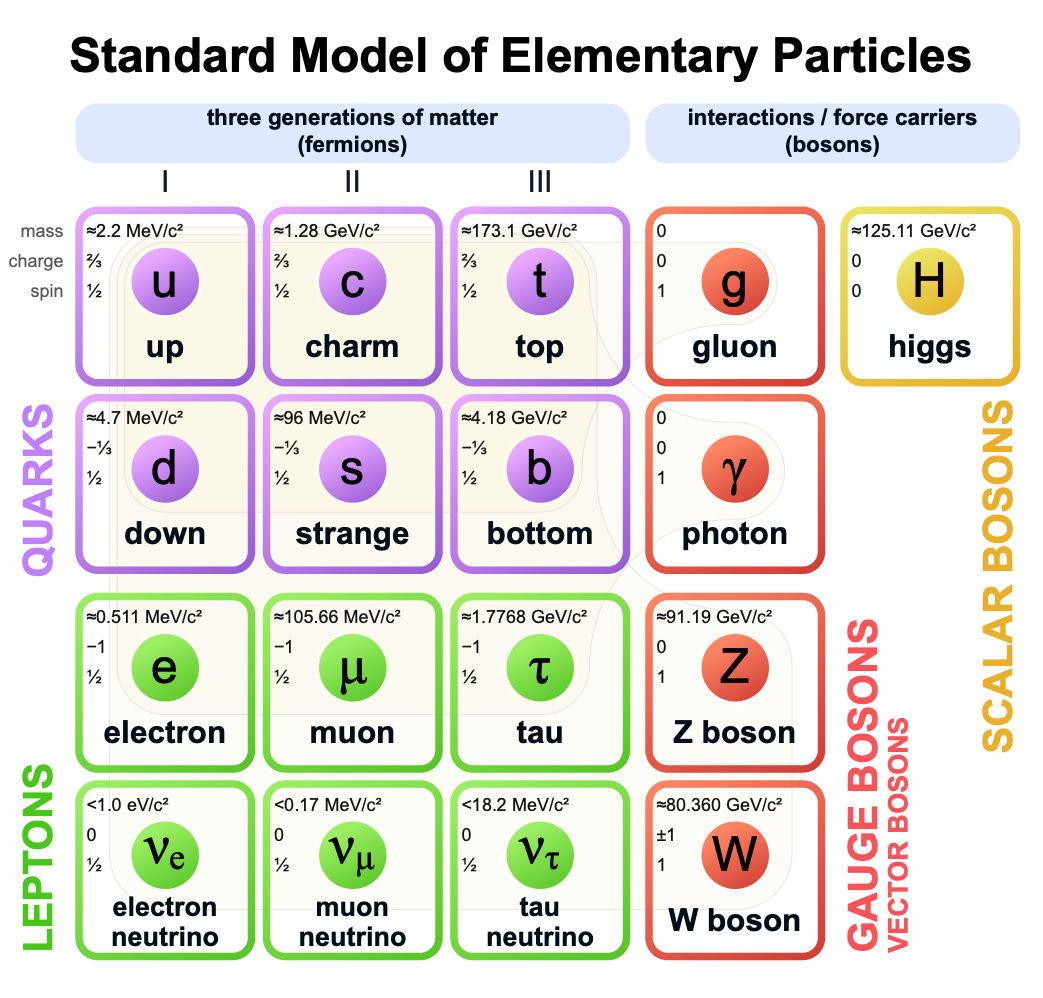
\includegraphics[width=8cm]{figures/ch-1-introduction/Standard_Model_of_Elementary_Particles.png}
    \caption{Table of Standard Model particles showing the grouping of the fermions into three generations of matter and the bosons, responsible for carrying the three fundamental forces in the Standard Model. The masses, charges, and spins of the particles are shown. The antimatter counterparts of the fermions are not shown. The possible interactions between the fermions and gauge bosons are highlighted.}
    \label{fig:intro-standard-model}
\end{figure}


Fermions consist of quarks and leptons, and are grouped into three generations. For example, the electron belongs to the first generation of leptons. The second and third generation counterparts of the electron are the muon and the tau lepton, and are over 200 and 30,000 times heavier than the electron respectively. Bosons are force carriers; the interaction of fermions with bosons corresponds to fundamental forces. The Standard Model describes the electromagnetic force, the strong nuclear force, and the weak nuclear force.


\section{The Standard Model as a gauge theory}
\label{section:SM-as-gauge-theory}

\subsection{Gauge invariance}
Gauge theories of elementary particle interactions originate from a freedom of choice in the mathematical description of particle fields which has no effect on the particles' physical states \cite{Tully+2012}. The existence and form of the particles' interactions, can be deduced from the existence of physically indeterminate, gaugable quantities.

An example of this gauge invariance is classical physics is the electromagnetic interaction, where the fundamental field is the four-vector potential $A^\mu$ \cite{Tully+2012}. The physical electromagnetic fields and Maxwell's equations arise from the elements of the tensor $F_{\mu\nu}(x) = \partial_\mu A_\nu (x) - \partial_\nu A_\mu (x)$. Any two choices of $A^\mu$ that are related by a transformation of the form

\begin{equation}
    A_\mu \rightarrow A_\mu + \partial_\mu \alpha
    \label{eqn:gauge_symmetry}
\end{equation} for any real, differentiable function $\alpha(x)$, describe the same physical configuration, and has no effect on Maxwell's equations. This ``redundancy'' in the choice of gauge in Eqn. \ref{eqn:gauge_symmetry} is called a gauge symmetry.

One important consequence of gauge symmetry comes from the application of Noether's theorem, which states that for every global transformation under which the Lagrangian density is invariant, there exists a conserved quantity. If $\mathcal{L}(\Psi(x), \partial_\mu \Psi(x))$ is invariant under the transformation of the wave function $\Psi(x) \rightarrow \Psi'(x)$, where $\Psi'(x) = \Psi(x) + \delta \Psi(x)$, then there exists a conserved current 
\begin{equation}
    \partial_\mu \left( \frac{\partial\mathcal{L}(x)}{\partial(\partial_\mu \Psi(x))} \delta \Psi(x)  \right) = 0
\end{equation}
In classical mechanics, the conservation of linear momentum, angular momentum, and energy follows from translational invariance, rotational variance, and invariance under translations in time \cite{Tully+2012}. Likewise, charge conservation can be shown to arise from the invariance of the Dirac Lagrangian density $\mathcal{L}_{\text{Dirac}} = \bar{\Psi} (i\gamma^\mu \partial_\mu -m)\Psi$ under the particle wavefunction's phase transformation, $\Psi'(x) = \exp(ie\chi) \Psi(x)$. Thus Noether's theorem establishes a correspondence between a gauge symmetry and a conserved internal property (e.g. charge or momentum).

\subsection{Local gauge symmetries}
Interactions between particles arise if we modify the wave function with a phase transformation $\Psi'(x) = \exp(i e \chi) \Psi(x)$, and allow the phase $\chi$ to be a function of spacetime \cite{Tully+2012}. A wave function of the form
\begin{equation}
    \Psi'(x) = \exp(i e \chi(x)) \Psi(x)
\end{equation}
can be verified to \textit{not} be a solution to the Dirac equation for free particles: $(i \gamma^\mu \partial_\mu - m) \Psi(x) = 0$. This necessitates a modified Dirac equation, where the derivative takes into account that the vector field $V(x)$ needs to be compared at two displaced space-time points in a curvilinear coordinate system: 
\begin{equation}
    \mathcal{D}_\mu \equiv \lim_{\Delta x^\mu \rightarrow 0} \frac{V_{\parallel}(x + \Delta x) - V(x)}
{\Delta x^\mu}\end{equation}
We define a covariant derivative, 
\begin{equation}
    D_\mu = \partial_\mu + i e A_\mu
\label{eqn:modified_dirac}
\end{equation}
where $A_\mu(x)$ is a 4-vector potential. Thus the modified Dirac equation reads:
\begin{equation}
    \left( i \gamma^\mu \mathcal{D}_\mu - m  \right) \Psi(x) = 0
\end{equation}
The simultaneous gauge transformation $A'_\mu(x) = A_\mu(x) - \partial_\mu\chi(x)$ and wavefunction transformation $\Psi'(x) = \exp(ie\chi(x)) \Psi(x)$ leaves the covariant-derivative form of the Dirac equation (Eqn \ref{eqn:gauge_symmetry}) invariant.

The generalization of this result is as follows: if a theory is invariant for unitary transformations $U$ of the particle states according to 
\begin{equation}
    \Psi' = U\Psi
\label{eqn:generic_unitary_transformation}
\end{equation}
One must define a derivative of the form
\begin{equation}
    D^\mu = \partial^\mu + ig B^\mu
\end{equation}
to keep the theory invariant under Eqn. \ref{eqn:generic_unitary_transformation}. The four-potential $B^\mu$ represents the interacting four-potential which must be added to keep the theory invariant.

In the case of the Standard Model, the theory is built around the gauge transformations $G = SU(3) \times SU(2) \times U(1)$. $SU(3)$ is associated to the strong force (subscripted $C$); $SU(2)$ is associated to the weak force (subscripted $L$); and $U(1)$ is hypercharge (subscripted Y). The gauge-covariant derivative  is 
\begin{equation}
    \mathcal{D}_\mu = \partial_\mu - ig' B_\mu \frac{Y}{2} - ig W_{\mu}^{\alpha} \frac{\tau_a}{2} - ig_s G_\mu^{k} \frac{\lambda_k}{2}
\end{equation}
\begin{itemize}
    \item In the $U(1)_Y$ term, $B_\mu$ is the weak hypercharge field.
    \item In the $SU(2)_L$ term, $W_\mu(x) = (W_\mu^1(x), W_\mu^2(x), W_\mu^3(x))$ are a triplet of four-potentials. $\tau/2$ are the Pauli matrices, generators of the $SU(2)$ transformation.
    \item In the $SU(3)_C$ term, the gluon (color) field is $G_\mu$. $\lambda_k$ are the Gell-Man matrices, generators of the $SU(3)$ transformation.
\end{itemize}   
The invariance of the Standard Model under $SU(3)_C \times SU(2)_L \times U(1)_Y$ requires massless fermions and massless force carriers.  

\section{The Higgs Mechanism}
\label{section:Higgs-mechanism}
To introduce mass into the theory, i.e. to change the propagation of the gauge particles and all the fermions, the physical vacuum cannot have all the symmetries of the Standard Model Lagrangian \cite{Tully+2012}. The symmetries of the physical vacuum must be spontaneously broken, without affecting gauge invariance in the Lagrangian. The Higgs mechanism proposes the existence of a scalar field, or fields, with nonzero vacuum expectation values, which reduce the gauge symmetries of the physical vacuum from $SU(3)_C \times SU(2)_L \times U(1)_Y$ down to $SU(3)_C \times U(1)_{EM}$.

The Higgs field interacts with the gauge bosons and fermions throughout space, impeding their free propagation. The resulting broken symmetry correctly predicts the mass ratio of the neutral (Z) and charged (W) massive electroweak bosons, and predicts that at least one physical degree of freedom in the Higgs field is a particle degree of freedom, called the Higgs boson. The location of the minimum of the Higgs potential can be constrained from previously measured Standard Model parameters, but the shape of the mass distribution of the Higgs boson must be experimentally measured.

The minimal choice of Higgs field comes from the breaking of $SU(2)_L \times U(1)_Y$ down to $U(1)_{EM}$. The smallest $SU(2)$ multiplet is the doublet. The existence of three massive electroweak bosons leads the Higgs sector to have at least three degrees of freedom. The minimal single-doublet complex scalar Higgs field is
\begin{equation}
    \Phi(x) = \begin{pmatrix} \phi^+(x) \\ \phi^0(x) \end{pmatrix} 
    = \frac{1}{\sqrt{2}} \begin{pmatrix} \phi_1^+(x) + i\phi_2^+(x) \\ \phi_1^0(x) + i\phi_2^0 (x) \end{pmatrix}
\end{equation}
where $\phi_1^+$, $\phi_2^+$, $\phi_1^0$, and $\phi_2^0$ are real (four degrees of freedom). By convention, the nonzero vacuum expectation value is assigned to $\phi_1^0$.

The minimal self-interacting Higgs potential that is invariant under $SU(2)_L \times U(1)_Y$ is given by
\begin{equation}
    V(\Phi^\dagger \Phi) = -\mu^2 \Phi^\dagger \Phi + \lambda (\Phi^\dagger \Phi)^2, \,\,\, \mu^2 > 0, \, \lambda > 0
\end{equation}
where $\lambda$ is the coupling strength of the four-point Higgs interaction. 
The potential energy is minimized at 
\begin{equation}
    \Phi_{\text{min}} = \frac{1}{\sqrt{2}} \begin{pmatrix} 0 \\ v \end{pmatrix}, \,\,\,\text{where} \, v = \sqrt{\mu^2 / \lambda}
\end{equation}
Choosing a fixed orientation of $\langle \Phi \rangle$ out of a continuous set of possible ground states spontaneously breaks the symmetry of the physical vacuum, as illustrated in Fig \ref{fig:higgs-potential}.

\begin{figure}[ht]
    \centering
    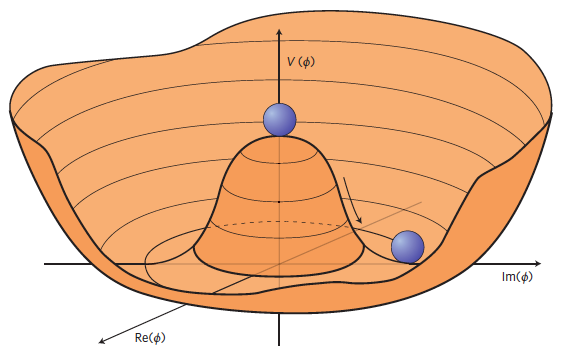
\includegraphics[width=8cm]{figures/ch-1-introduction/higgs-potential.png}
    \caption[An illustration of the Higgs potential.]{An illustration of the Higgs potential \cite{Ellis:2013jnq}. Choosing any of the points at the bottom of the potential breaks spontaneously the rotational $U(1)$ symmetry.}
    \label{fig:higgs-potential}
\end{figure}

The excitations of the Higgs field with respect to the minimum $\Phi_{\text{min}}$ are parameterized by 
\begin{equation}
    \Phi(x) = \exp(i \boldsymbol{\xi}(x) \cdot \boldsymbol{\tau}) \frac{1}{\sqrt{2}} \begin{pmatrix} 0 \\ v + H(x) \end{pmatrix}
\end{equation}
Three degrees of freedom are coupled directly to the electroweak gauge bosons; this is often referred to as the gauge bosons ``eating'' the Goldstone bosons to form the longitudinal polarizations of the massive spin-1 boson states. The $H(x)$ excitation is in the radial direction and corresponds to the free particle state of the Higgs boson. 

\section{Two-Higgs Doublet Models}
\label{section:theory-2HDM}

One of the simplest possible extensions to the Standard Model is adding a doublet to the minimal Higgs sector of the Standard Model, which is a $SU(2)_L$ doublet $H$ with hypercharge $Y = +\frac{1}{2}$, denoted here as $H \sim 2_{+1/2}$. These extensions are found in several theories such as supersymmetry. A general 2HDM can be extended with a light scalar (2HDM+S) to obtain a rich set of exotic Higgs decays \cite{2HDM-PhysRevD.90.075004}. 

The charges of the Higgs fields are chosen to be $H_1 \sim 2_{-1/2}$ and $H_2 \sim 2_{+1/2}$, which acquire vacuum expectation values $v_{1,2}$ which are assumed to be real and aligned \cite{2HDM-PhysRevD.90.075004}. Expanding about the minima yields two complex and four real degrees of freedom:
\begin{align}
    H_1 &= \frac{1}{\sqrt{2}} \begin{pmatrix} v_1 + H^{0}_{1, R} + iH^0_{1, I} \\  
                                              H^-_{1,R} + i H^-_{1, I}   \end{pmatrix} \\
    H_2 &= \frac{1}{\sqrt{2}} \begin{pmatrix} H^+_{2, R} + iH^+_{2, I} \\  
                                              v_2 + H^0_{2,R} + i H^0_{2, I}   \end{pmatrix} 
\end{align}

The charged scalar and pseudoscalar mass matrices are diagonalized by a rotation angle $\beta$, defined as $\tan\beta = v_2/v_1$. One charged (complex) field and one neutral pseudoscalar combination of $H^0_{1, 2, I}$ are eaten by the SM gauge bosons after electroweak symmetry breaking \cite{2HDM-PhysRevD.90.075004}. The other complex field yields two charged mass eigenstates $H^\pm$, which are assumed to be heavy. The remaining three degrees of freedom yield one neutral pseudoscalar mass eigenstate 
\begin{equation}
    A = H^0_{1, I}\sin\beta - H^0_{2, I} \cos\beta
\end{equation}
and two neutral scalar mass eigenstates (where $-\pi/2 \leq \alpha \leq pi/2$)
\begin{equation}
    \begin{pmatrix} h \\ H^0 \end{pmatrix} = \begin{pmatrix} -\sin\alpha & \cos\alpha \\
                                                              \cos\alpha & \sin\alpha \end{pmatrix}
                                             \begin{pmatrix} H^0_{1, R} \\ H^0_{2, R}  \end{pmatrix}
\end{equation}
We assume that the 2HDM is near or in the decoupling limit: $\alpha \rightarrow \pi/2 - \beta$, where the lightest state in the 2HDM is $h$, which we identify as the 125 GeV Higgs particle \cite{2HDM-PhysRevD.90.075004}. In this limit, the fermion couplings of $h$ become identical to the Standard Model Higgs, while the gauge boson couplings are very close to Standard Model-like for $\tan\beta \gtrsim 5$. All of the properties of $h$ are determined by just two parameters: $\tan\beta$ and $\alpha$, and the fermion couplings to the two Higgs doublets. 

2HDM can be extended by a scalar singlet (2HDM+S) \cite{2HDM-PhysRevD.90.075004}:
\begin{equation}
    S = \frac{1}{\sqrt{2}} (S_R + iS_I)
\end{equation}
If this singlet only couples to the Higgs doublets $H_{1,2}$ and has no direct Yukawa couplings, all of its couplings to SM fermions result from mixing with $H_{1,2}$. Under these simple assumptions, exotic Higgs decays $h\rightarrow ss \rightarrow X\bar{X}Y\bar{Y}$ or $h\rightarrow aa \rightarrow X\bar{X}Y\bar{Y}$, and $h \rightarrow aZ \rightarrow X\bar{X}Y\bar{Y}$ are permitted, where $s(a)$ is a (pseudo)scalar mass eigenstate mostly composed of $S_R (S_I)$, and $X, Y$ are Standard Model fermions or gauge bosons. There are two pseudoscalars in the 2HDM+S, and the mostly singlet-like pseudoscalar can be chosen to be the one lighter than the SM-like Higgs. For $m_a < m_h - m_Z \sim 35$ GeV, the exotic Higgs decay $h \rightarrow Za$ is possible, and for $m_a < m_h/2 \approx 63$ GeV, the exotic Higgs decay $h \rightarrow aa$ is possible. 

\begin{figure}[ht]
    \centering
    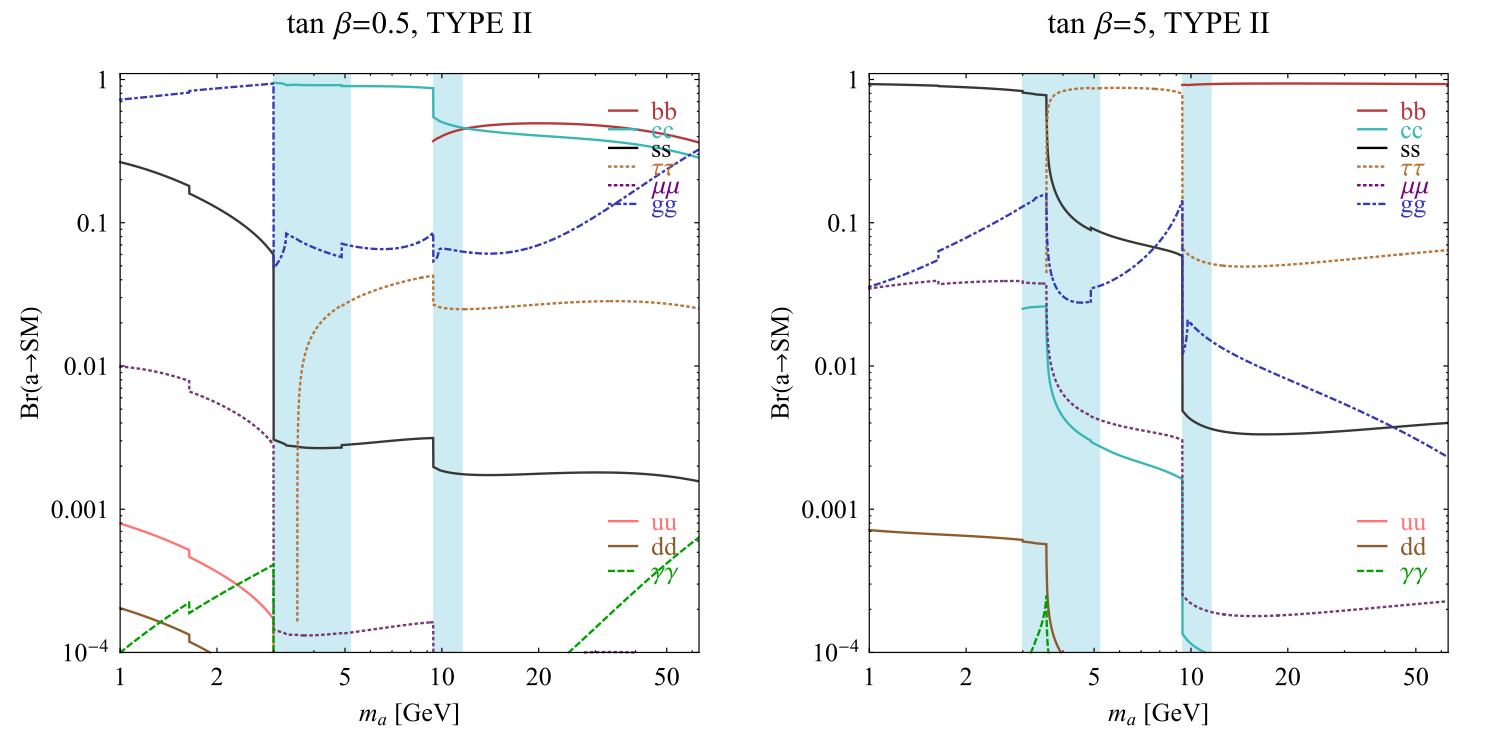
\includegraphics[width=15cm]{figures/ch-1-introduction/curtin-2014-figure-7-BRs-of-singlelike-pseudoscalar-type-II.png}
    \caption[Branching ratios of a singlet-like pseudoscalar in Type II 2HDM+S for $\tan\beta = 0.5$ (left) and $\tan\beta = 5$ (right).]{Branching ratios of a singlet-like pseudoscalar in Type II 2HDM+S for $tan\beta = 0.5$ (\textit{left}) and $\tan\beta = 5$ (\textit{right}) from \cite{2HDM-PhysRevD.90.075004}, showing the dependence of the branching ratios on $\tan\beta$, as well as the prominence of the branching ratios to $bb$ and $\tau\tau$, the channels searched for in the analysis presented here.}
    \label{fig:curtin-2014-fig-4-typeI-BRs}
\end{figure}


In 2HDM, and by extension 2HDM+S, there are four types of fermion couplings commonly discussed in the literature that forbid flavor-changing neutral currents at tree level \cite{2HDM-PhysRevD.90.075004}. These are referred to as Type I (all fermions couple to $H_2$), Type II (MSSM-like, $d_R$ and $e_R$ couple to $H_1$, $u_R$ to $H_2$), Type III (lepton-specific, leptons and quarks couple to $H_1$ and $H_2$ respectively) and Type IV (flipped, with $u_R$, $e_R$ coupling to $H_2$ and $d_R$ to $H_1$). The exact branching ratios of the pseudoscalars to Standard Model particles vary depending on the 2HDM+S model and the value of $\tan\beta$ (e.g. Fig. \ref{fig:curtin-2014-fig-4-typeI-BRs}).

\section{Two Real Singlet Model}
\label{section:theory-TRSM}
The two real singlet model (TRSM) adds two real singlet degrees of freedom to the Standard Model. These are written as two real singlet fields $S$ and $X$. Depending on the vacuum expectation values acquired by the scalars, different phases of the model can be realized \cite{Robens:2019kga}. To reduce the number of free parameters, two discrete $\mathbb{Z}_2$ symmetries are introduced. The fields are decomposed as

\begin{equation}
    \Phi = \begin{pmatrix} 0 \\ \frac{\phi_h + v}{\sqrt{2}} \end{pmatrix}, 
    \,
    S = \frac{\phi_S + v_S}{\sqrt{2}} ,
    \,
    X = \frac{\phi_X + v_X}{\sqrt{2}}
\end{equation}
To achieve electroweak-breaking symmetry, $v  = v_{SM} \sim 246$ 246 GeV is necessary. If the vacuum expectation values $v_S, v_X \neq 0$ the $\mathbb{Z}_2$ are spontaneously broken, and the fields $\phi_{h,S,X}$ mix into three physical scalar states. This is called the broken phase and leads to the most interesting collider phenomenology.

The mass eigenstates $h_{1,2,3}$ are related to the fields $\phi_{h,S,X}$ through a $3\times 3$ orthogonal mixing matrix denoted $R$. The mass eigenstates are assumed to be ordered $M_1 \leq M_2 \leq M_3$. $R$ is parameterized by the three mixing angles $\theta_{hS}$, $\theta_{hX}$, $\theta_{SX}$. The nine parameters of the scalar potential can be expressed in terms of the three physical Higgs masses, the three mixing angles, and the three vacuum expectation values. 

After fixing one of the Higgs masses to the mass of the observed Higgs boson, and fixing the Higgs doublet vacuum expectation value to its Standard Model value, there are seven remaining free parameters of the TRSM \cite{Robens:2019kga}.

In one benchmark scenario of TRSM \cite{Robens:2019kga}, the heaviest scalar state $h_3$ is identified with the 125 GeV Higgs, $h_{125}$, and it can decay asymmetrically $h_{125} \rightarrow h_1 h_2$, which we also denote $h \rightarrow a_1 a_2$ to highlight the similarity with the symmetric decay $h \rightarrow aa$ typically interpreted in 2HDM+S as discussed. The parameter values in TRSM are chosen such that the coupling of $h_3$ to Standard Model particles are nearly identical to the Standard Model predictions. 

\begin{figure}[ht]
    \centering
    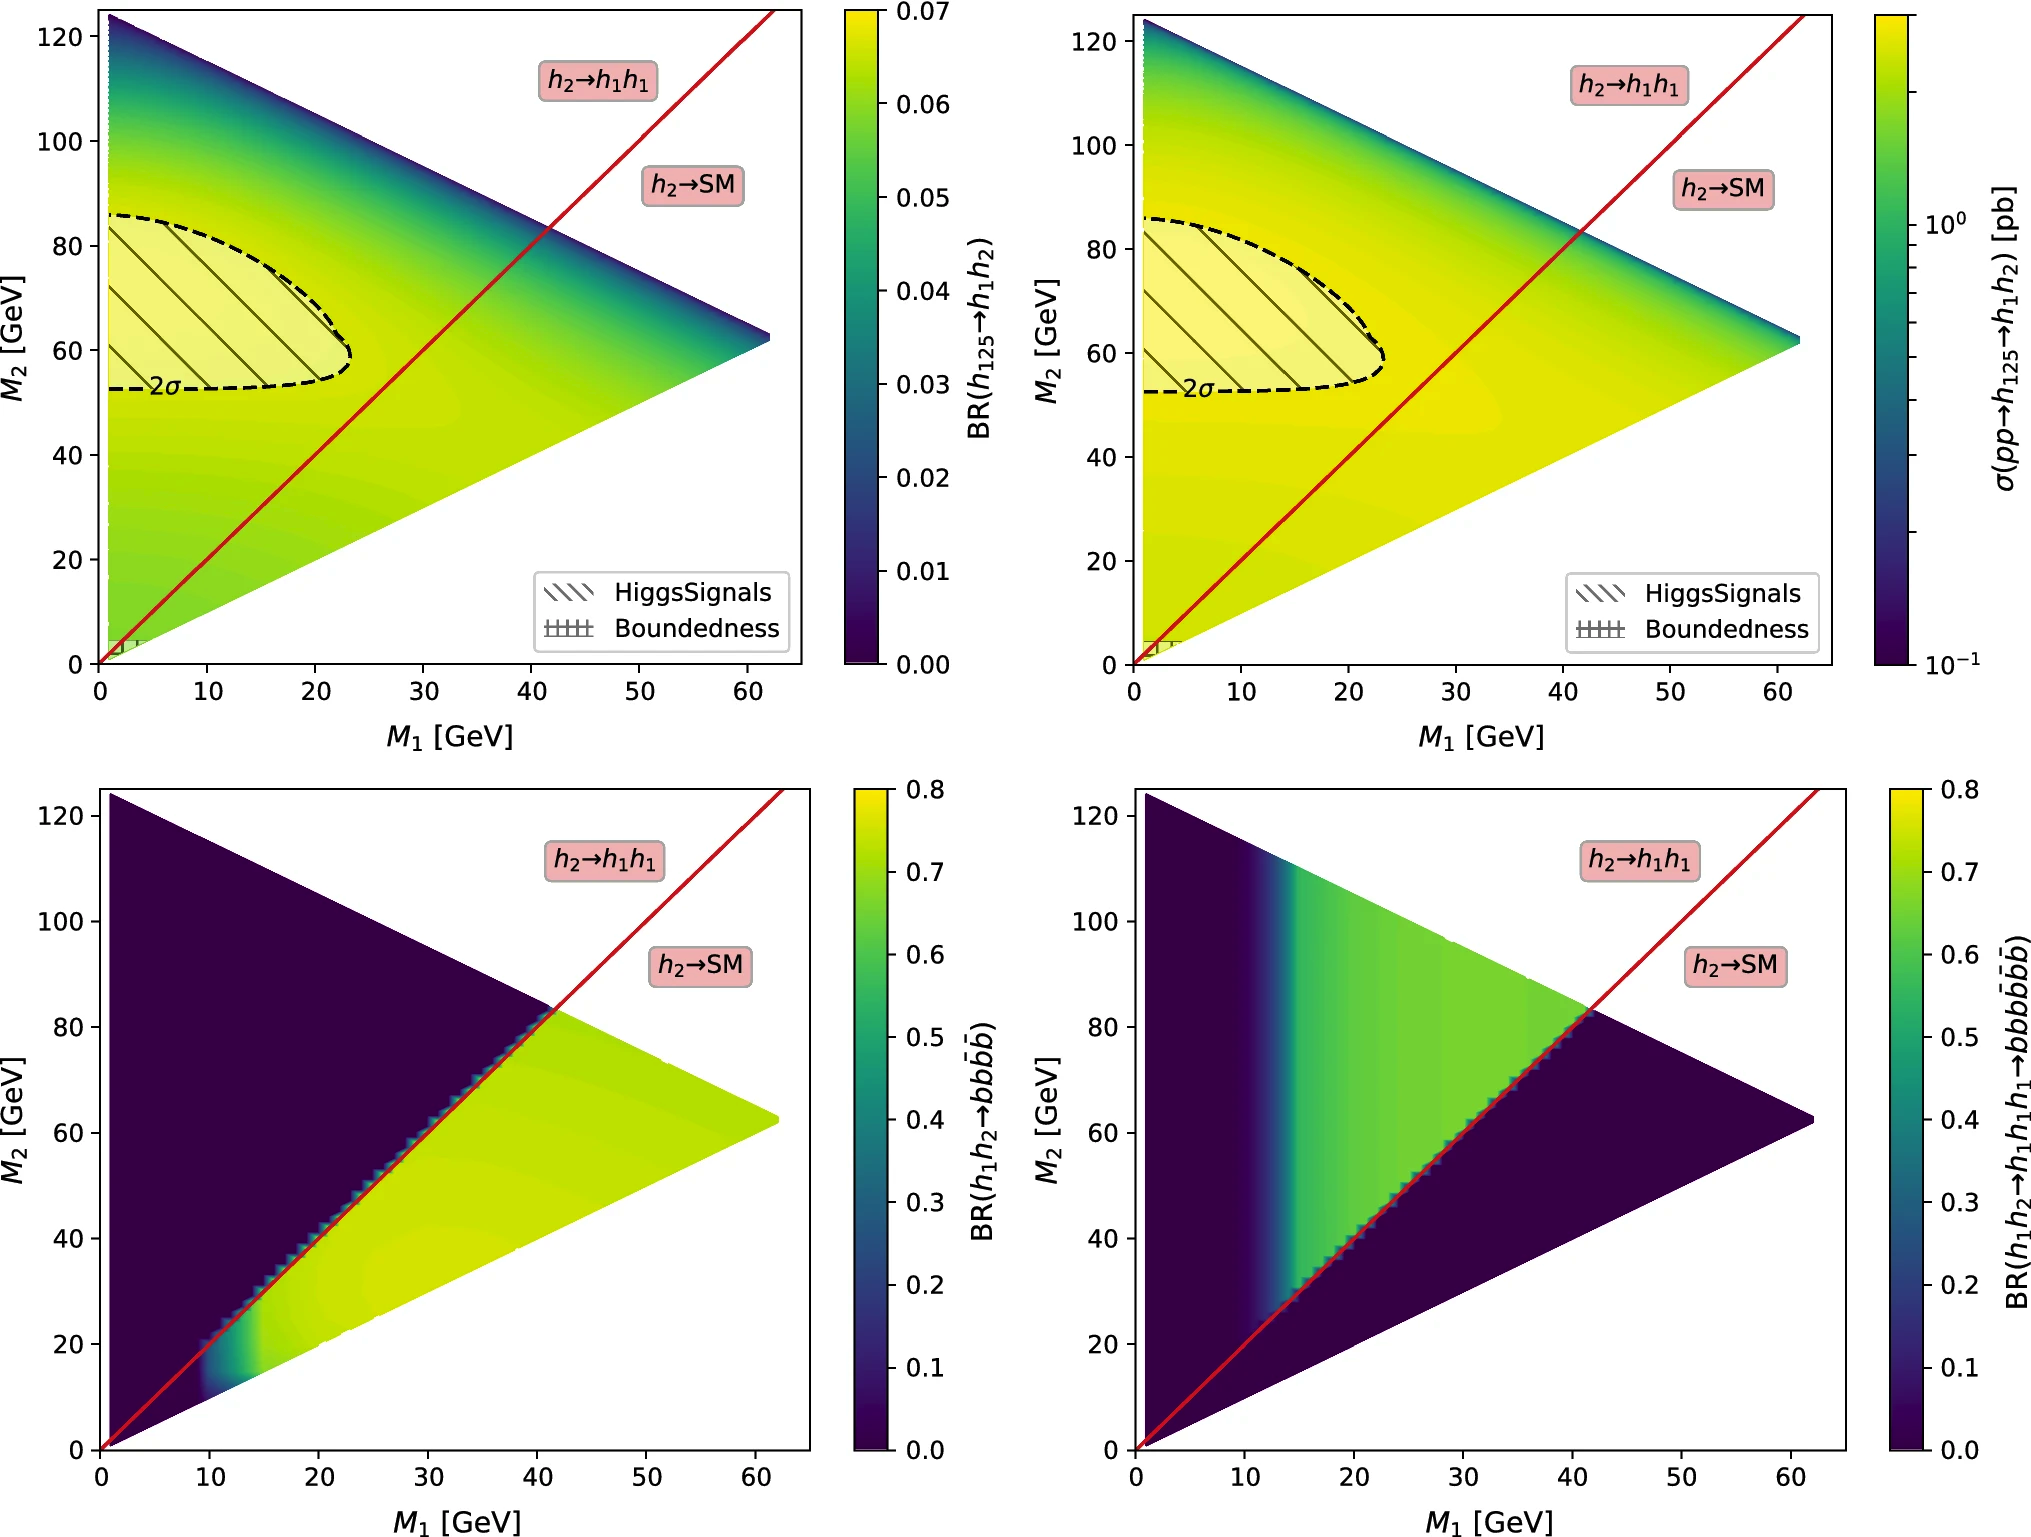
\includegraphics[width=15cm]{figures/ch-1-introduction/Robens-TRSM-Figure-6-BP-1.png}
    \caption[Benchmark plane BP1 for benchmark scenario 1, for the decay signature $h_{125} \rightarrow h_1 h_2$ with $h_{125} \equiv h_3$, defined in the $(M_1, M_2)$ plane.]{Benchmark plane BP1 for benchmark scenario 1 from \cite{Robens:2019kga}, for the decay signature $h_{125} \rightarrow h_1 h_2$ with $h_{125} \equiv h_3$, defined in the $(M_1, M_2)$ plane. The color code shows BR$(h_3 \rightarrow h_1 h_2)$ (\textit{top left}) and the 13 TeV LHC signal rate for $pp \rightarrow h_3 \rightarrow h_1 h_2$ (\textit{top right}). The red line separates the region $M_2 > 2 M_1$, where BR($h_2 \rightarrow h_1 h_1$) $\sim 100\%$, from the region $M_2 < 2 M_1$, where BR($h_2 \rightarrow F_{SM}$) $\sim 100\%$. The \textit{bottom left} and \textit{right} show the branching ratio of the $h_1 h_2$ into (respectively) $b\bar{b}b\bar{b}$, and through a $h_2 \rightarrow h_1 h_1$ cascade to $b\bar{b}b\bar{b}b\bar{b}$. The hatched region indicates where the decay rate slightly exceeds the $2\sigma$ upper limit inferred from the LHC Higgs rate measurements, though the region depends on the parameter choices and experimental searches should cover the whole mass range.}
    \label{fig:trsm_bp1}
\end{figure}

In benchmark scenario 1 (benchmark plane 1, or BP1) (Fig. \ref{fig:trsm_bp1}) \cite{Robens:2019kga}, the maximal branching ratios for $h_3 \rightarrow h_1 h_2$ reach up to $7-8\%$ which translates into a signal rate of around 3 pb. These maximal branching ratios are reached in the intermediate mass state for $h_2$, $M_2 \sim 60 - 80$ GeV. For $M_2 < 40$ GeV, although phase space opens up significantly for light decay products, the branching ratio becomes smaller. 

If the decay channel $h_2 \rightarrow h_1 h_1$ is kinematically open (i.e. $M_2 > 2M_1$), it is the dominant decay mode leading to a significant rate for the $h_1 h_1 h_1$ final state, in a ``cascade" decay. In BP1, $BR(h_2 \rightarrow h_1h_1$) $\simeq 100\%$ above the red line in Fig. \ref{fig:trsm_bp1}. If, in addition, $M_1 \gtrsim 10$ GeV, the $h_1$ decays dominantly to $b\bar{b}$ leading to a sizable rate for the $b\bar{b}b\bar{b}b\bar{b}$ final state as shown in Fig. \ref{fig:trsm_bp1} (\textit{bottom right}).

If the $h_2 \rightarrow h_1 h_1$ decay is kinematically closed (i.e. $M_2 < 2M_1$), both scalars decay directly to Standard Model particles, with branching ratios identical to a Standard Model-like Higgs boson, i.e. with the $b\bar{b}b\bar{b}$ final state dominating, as shown in Fig. \ref{fig:trsm_bp1} (\textit{bottom left}), while at smaller masses, combinations with $\tau$ leptons and eventually final states with charm quarks and muons become relevant \cite{Robens:2019kga}.


\chapter{The Large Hadron Collider and the CMS Experiment}
This chapter introduces the key aspects of the CERN Large Hadron Collider (LHC) and the Compact Muon Solenoid (CMS) experiment where the work for this thesis was conducted. Section \ref{section:LHC} describes the history of accelerator developments at CERN that led to the construction of the LHC, the current LHC configuration, and the largest experiments located at the LHC. The concepts of beam luminosity and pileup, which are critical for understanding and measuring high-energy particle collisions, are described in Section \ref{section:luminosity_and_pileup} and discussed in the context of the High-Luminosity LHC (HL-LHC) upgrade in Section \ref{section:HL-LHC}. Lastly, Section \ref{section:cms-detector} describes the design and function of CMS and its subdetectors, and terminates in a description of data processing at CMS, beginning from online event filtering in the Level-1 Trigger, to processing in the High-Level Trigger, to offline particle reconstruction, and finally long-term storage and processing of measured events.

\section{The Large Hadron Collider}
\label{section:LHC}
CERN, the European Organization for Nuclear Research, is an international organization based in Meyrin, Switzerland which operates the world's largest particle physics laboratory, and is the site of the Large Hadron Collider (LHC) \cite{history_of_CERN}. The very first accelerator built at CERN was the 600 MeV Synchrocyclotron (SC), which initially provided beams for CERN's first experiments. The newer and more powerful Proton Synchrotron (PS), which could accelerate particles to an energy of 28\GeV, began operations in 1959 and is still in use today. The first hadron collider at CERN was the Intersecting Storage Rings (ISR), which consisted of two interlaced rings each with a diameter of 200. The ISR collided protons at a center-of-mass energy of 62\GeV and began measuring collisions in 1971. In 1968 CERN began to accelerate heavy ions in the Super Proton Synchrotron (SPS), which is 7 kilometers in circumference and was the first of CERN's giant underground rings to be built. The SPS became the forefront of CERN's particle physics program in 1976, and in 1981 was converted into a proton-antiproton collider. The final and largest underground ring constructed at CERN was the Large Electron-Positron (LEP) collider, which was commissioned in July 1989 and hosted 5176 magnets and 128 accelerating cavities located around a 27-kilometer circumference. Over 11 years of research, four detectors, ALEPH, DELPHI, L3, and OPAL measured the collisions, with collision energies reaching up to 209\GeV in the year 2000. In November 2000, LEP was closed down to make way for the construction of the LHC in the same tunnel.

In its current configuration, the LHC accelerator complex at CERN is a succession of machines that accelerate particles in stages until they reach their final energy of 6.5 TeV per beam \cite{CERN-OPEN-2000-148} \cite{Linac4-design-report-2020}. In Linear accelerator 4 (Linac4), negative hydrogen ions (hydrogen atoms with an additional electron) are accelerated to 160 MeV, and stripped of their two electrons, leaving only protons, before entering the Proton Synchrotron Booster (PSB). These protons are accelerated to 2\GeV, then to 26\GeV in the Proton Synchrotron (PS), and 450\GeV in the Super Proton Synchrotron (SPS). The protons are transferred to the two beam pipes of the Large Hadron Collider (LHC). The LHC is a 27-kilometer ring of superconducting magnets, inside which one beam circulates clockwise and the other counterclockwise. Each LHC ring takes 4 minutes and 20 seconds to fill, and it takes about 20 minutes for the protons to reach their maximum energy. During normal operating conditions, beams circulate for many hours inside the LHC ring. 

The beams of particles in the LHC are made to collide at a center-of-mass energy of up to 14 TeV, at four positions at particle detector experiments located around the ring: ATLAS, CMS, ALICE, and LHCb. An aerial view of the four major experiments' locations is shown in Fig. \ref{fig:aerial-view-LHC-ring} \cite{OPEN-PHO-ACCEL-2017-005}. ATLAS and CMS are the two general-purpose detectors with broad physics programmes spanning Standard Model measurements and searches for signatures of new physics \cite{ATLAS-TDR-14} \cite{CERN-LHCC-2006-001}. The two experiments use different technical solutions and different magnet system designs. ALICE is a general-purpose detector dedicated to measuring LHC heavy-ion collisions, and is designed to address the physics of strongly interacting matter, and the properties of quark-gluon plasma \cite{ALICE-original-TDR}. The LHCb experiment specializes in investigating CP violation through measuring the differences in matter and antimatter, by using a series of subdetectors to detect mainly forward particles close to the beam direction \cite{LHCb-1998}. 

\begin{figure}[ht]
    \centering
    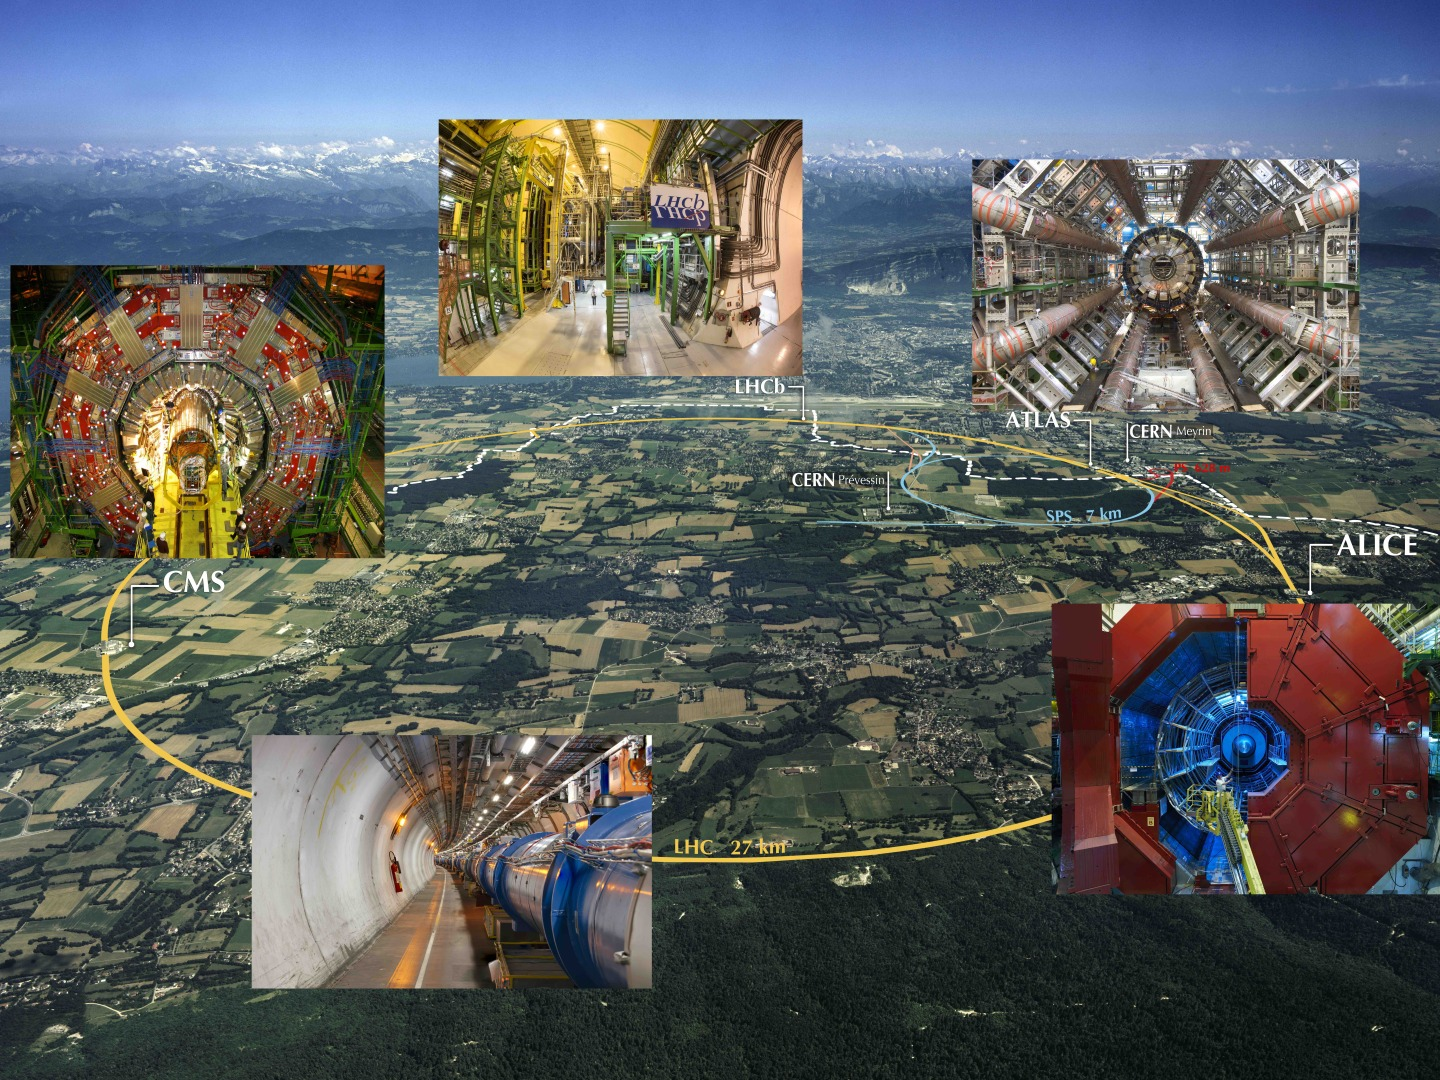
\includegraphics[width=11cm]{figures/ch-2-cern-cms/aerial-view-LHC-ring.jpeg}
    \caption[Aerial view of the Large Hadron Collider (LHC).]{Aerial view of the Large Hadron Collider (LHC) spanning the border of France and Switzerland, and the four major experiments located around the ring: CMS (Compact Muon Solenoid), LHCb (LHC beauty), ATLAS (A Toroidal LHC Apparatus), and ALICE (A Large Ion Collider Experiment) \cite{OPEN-PHO-ACCEL-2017-005}.}
    \label{fig:aerial-view-LHC-ring}
\end{figure}



\section{Luminosity and pileup}
\label{section:luminosity_and_pileup}
In order to search for rare decays, such as those that result from the creation and decay of a Higgs, W, or Z boson, a large number of parton interactions per second are required at the LHC. The number of events generated per second by the LHC collisions is given by
\begin{equation}
     N_{event} = \mathcal{L} \cdot \sigma_{event}
    \label{eqn:nEvents}
\end{equation} 
where $\sigma_{event}$ is the cross-section for the event under study, and $\mathcal{L}$ the instantaneous luminosity. The instantaneous luminosity is measured in units of cm$^{-2}$ s$^{-1}$, and depends only on the beam parameters, and can be written for a Gaussian beam distribution as:
\begin{equation}
    \mathcal{L} = \frac{N_b^2 n_b f_{rev} \gamma_r}{4\pi \epsilon_n \beta^*} F
\end{equation}
where the parameters are as defined, along with some example typical nominal values in Phase-1 of the LHC \cite{CERN-luminosity-accelerator-school-article} \cite{ipac2012-proceedings}:
% reference: material included in introduction to accelerator physics 2021 https://indico.cern.ch/event/1001431/contributions/

\begin{itemize}
    \item $N_b$ is the number of particles per bunch ($N_b \approx 1.15 \times 10^{11}$ protons per bunch)
    \item $n_b$ is the number of bunches per beam (maximum 2808),
    \item $f_{rev}$ is the revolution frequency ($\approx 11$ kHz),
    \item $\gamma_r$ is the relativistic gamma factor,
    \item $\epsilon_n$ is the normalized transverse beam emittance (area in a transverse plane occupied by the beam particles),
    \item $\beta^*$ is the beta function at the collision point ($\beta^* = 0.55$ m),
    \item and $F$ is the geometric luminosity reduction factor due to the crossing angle at the interaction points ($F \approx 0.84$ for Phase-1. Note that complete overlap would give $F = 1$).
\end{itemize}
Peak luminosity at interaction points 1 and 5 reach values of $\sim 1.0 \times 10^{34}$ cm$^{-2}$ s$^{-1}$, with peak luminosity per bunch crossing reaching $\sim 3.56 \times 10^{34}$ cm$^{-2}$ s$^{-1}$.

Per Eqn. \ref{eqn:nEvents}, the integrated luminosity over time is proportional to the number of events produced, and the size of LHC datasets is commonly presented in terms of integrated luminosity. Collider operation aims to optimize the integrated luminosity. Thus the exploration of rare events in the LHC collisions requires both high beam energies and high beam intensities.

The LHC's nominal beam luminosities are sufficiently large for multiple proton-proton collisions to occur in the same time window of 25 nanoseconds in which proton bunches collide \cite{CMS-JME-18-001}. These multiple collisions will lead to particle interactions overlapping in the detector. To measure a proton-proton collision, the single collision must be separated from overlapping collisions, which are called ``pileup'' collisions. A distribution of pileup in the data-taking years 2016-2018 is shown in Fig. \ref{fig:pileup-run-2}. The pileup is defined as the average number of $pp$ collisions per bunch crossing.

CMS reports an inelastic $pp$ cross section of $\sigma_{\text{inel}} = 68.6$ millibarns at a center-of-mass energy of $\sqrt{s} = 13$ TeV \cite{CERN-EP-2018-004-pileup}, which can be used to estimate pileup as follows:
\begin{equation}
    \text{Pileup} = \frac{\mathcal{L} \times \sigma_{\text{inel}}}{ n_b \cdot f}
\end{equation}
With the example values above, pileup can be estimated to be $\sim 22$.

Thus, higher luminosities create more intense pileup conditions, posing a greater challenge to detector performance and particle reconstruction and identification.

\begin{figure}[ht]
    \centering
    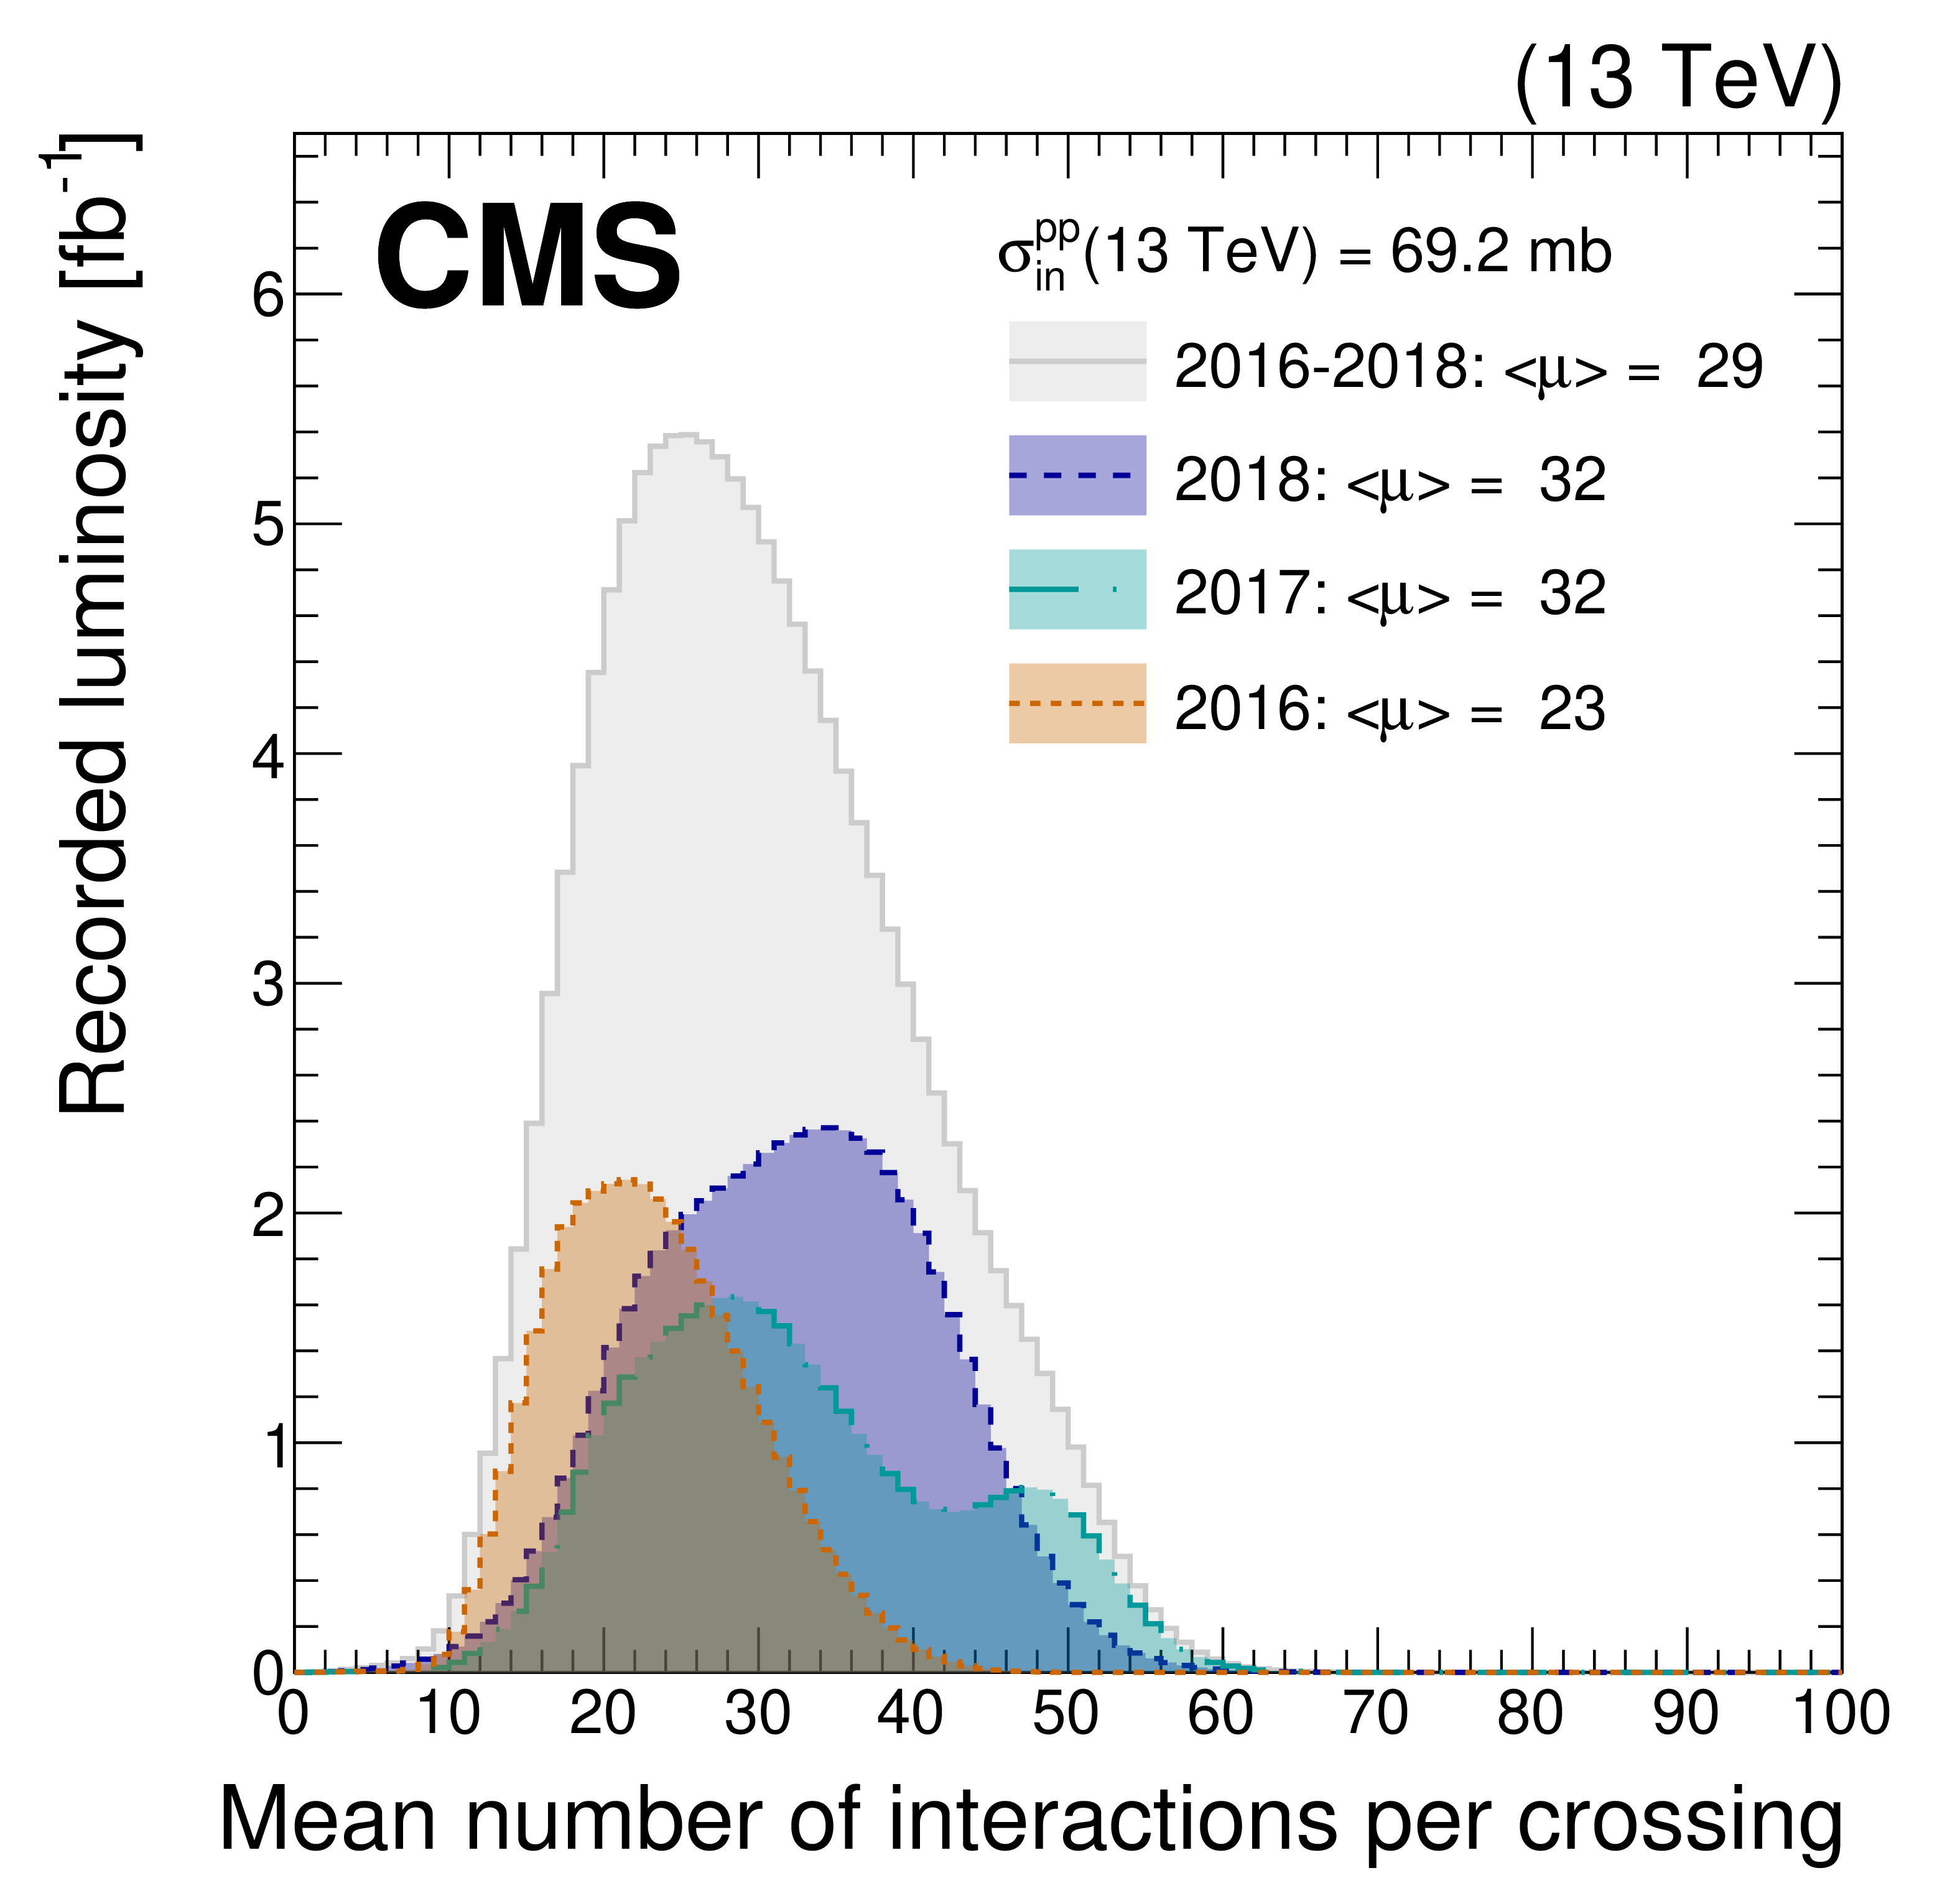
\includegraphics[width=8cm]{figures/ch-2-cern-cms/pileup-run-2-CMS-JME-18-001_Figure_001.png}
    \caption[Distribution of the mean number of inelastic collisions per bunch crossing (pileup) in data, for proton-proton collisions in 2016-2018]{Distribution of the mean number of inelastic collisions per bunch crossing (pileup) in data \cite{CMS-JME-18-001}, for proton-proton collisions in 2016 (\textit{dotted orange}), 2017 (\textit{dotted light blue}), 2018 (\textit{dotted dark blue}), and integrated over 2016-2018 (\textit{solid grey}). A cross-section of inelastic proton-proton collisions of 69.2 mbarns is assumed. In the running conditions of the High-Luminosity LHC, pileup will reach unprecedented levels of up to 200 per bunch crossing \cite{CERN-2020-010-HL-LHC-TDR}.}
    \label{fig:pileup-run-2}
\end{figure}

\section{The High-Luminosity LHC}
\label{section:HL-LHC}
The High-Luminosity LHC (HL-LHC) is a major upgrade of the LHC scheduled to take place in the late 2020s, that will increase the instantaneous luminosity by a factor of of five beyond the original design value, and the integrated luminosity by a factor of ten \cite{CERN-2020-010-HL-LHC-TDR}. This will be accomplished through accelerator technological advances: for instance, reduction of the interaction point $\beta^*$ from 0.55 m down to 0.15 m by installation of new final-focusing magnets, and improvements in the geometric luminosity loss factor $F \approx 1$ through the installation of crab cavities that optimize the orientation of colliding bunches. A further discussion of the HL-LHC upgrades for the CMS detector follows in Chapter \ref{chapter:ch-3:phase-2-upgrade-cms}.

\section{The CMS Detector}
\label{section:cms-detector}

The Compact Muon Solenoid (CMS) experiment was conceived to study proton-proton and lead-lead collisions at a center-of-mass energy of 14 TeV (5.5 TeV nucleon-nucleon) and at luminosities up to $10^{34}$ cm$^{-2}$ s$^{-1}$ ($10^{27}$ cm$^{-2}$ s$^{-1}$) \cite{CMS-2008-JINST-3-S08004} \cite{CERN-EP-2017-110}. Starting from the beam interaction region at the center of the CMS detector, particles first pass through a silicon pixel and strip tracker, in which charged-particle trajectories (tracks) and origins (vertices) are reconstructed from signals (hits) in the sensitive layers. The tracker is immersed in a high-magnetic-field superconducting solenoid that bends the trajectories of charged particles, allowing the measurement of their electric charge and momenta. Electrons and photons are then absorbed in an electromagnetic calorimeter (ECAL) comprised of lead-tungstate scintillating-crystals. The corresponding electromagnetic showers are detected as clusters of energy recording in neighboring cells, from which the direction and energy of the particles can be determined. Charged and neutral hadrons may initiate a hadronic shower in the ECAL as well, which is then fully absorbed in the hadron calorimeter (HCAL). The resulting clusters are used to estimate their direction and energies. Muons and neutrinos pass through the calorimeters with little to no interactions. Neutrinos escaped undetected; muons produce hits in additional gas-ionization chamber muon detectors housed in the iron yoke of the flux-return. A sketch of example particle interactions in a transverse slice of the CMS detector is shown in Fig. \ref{fig:sketch-cms-particle-interactions}. The collision data is recorded with the use of the Level-1 (L1) trigger (discussed in greater detail in \ref{section:phase-1-l1-trigger}), the High-Level Trigger (HLT), and data acquisition systems ensuring high efficiency in selecting physics events of interest. 

\begin{figure}[ht]
    \centering
    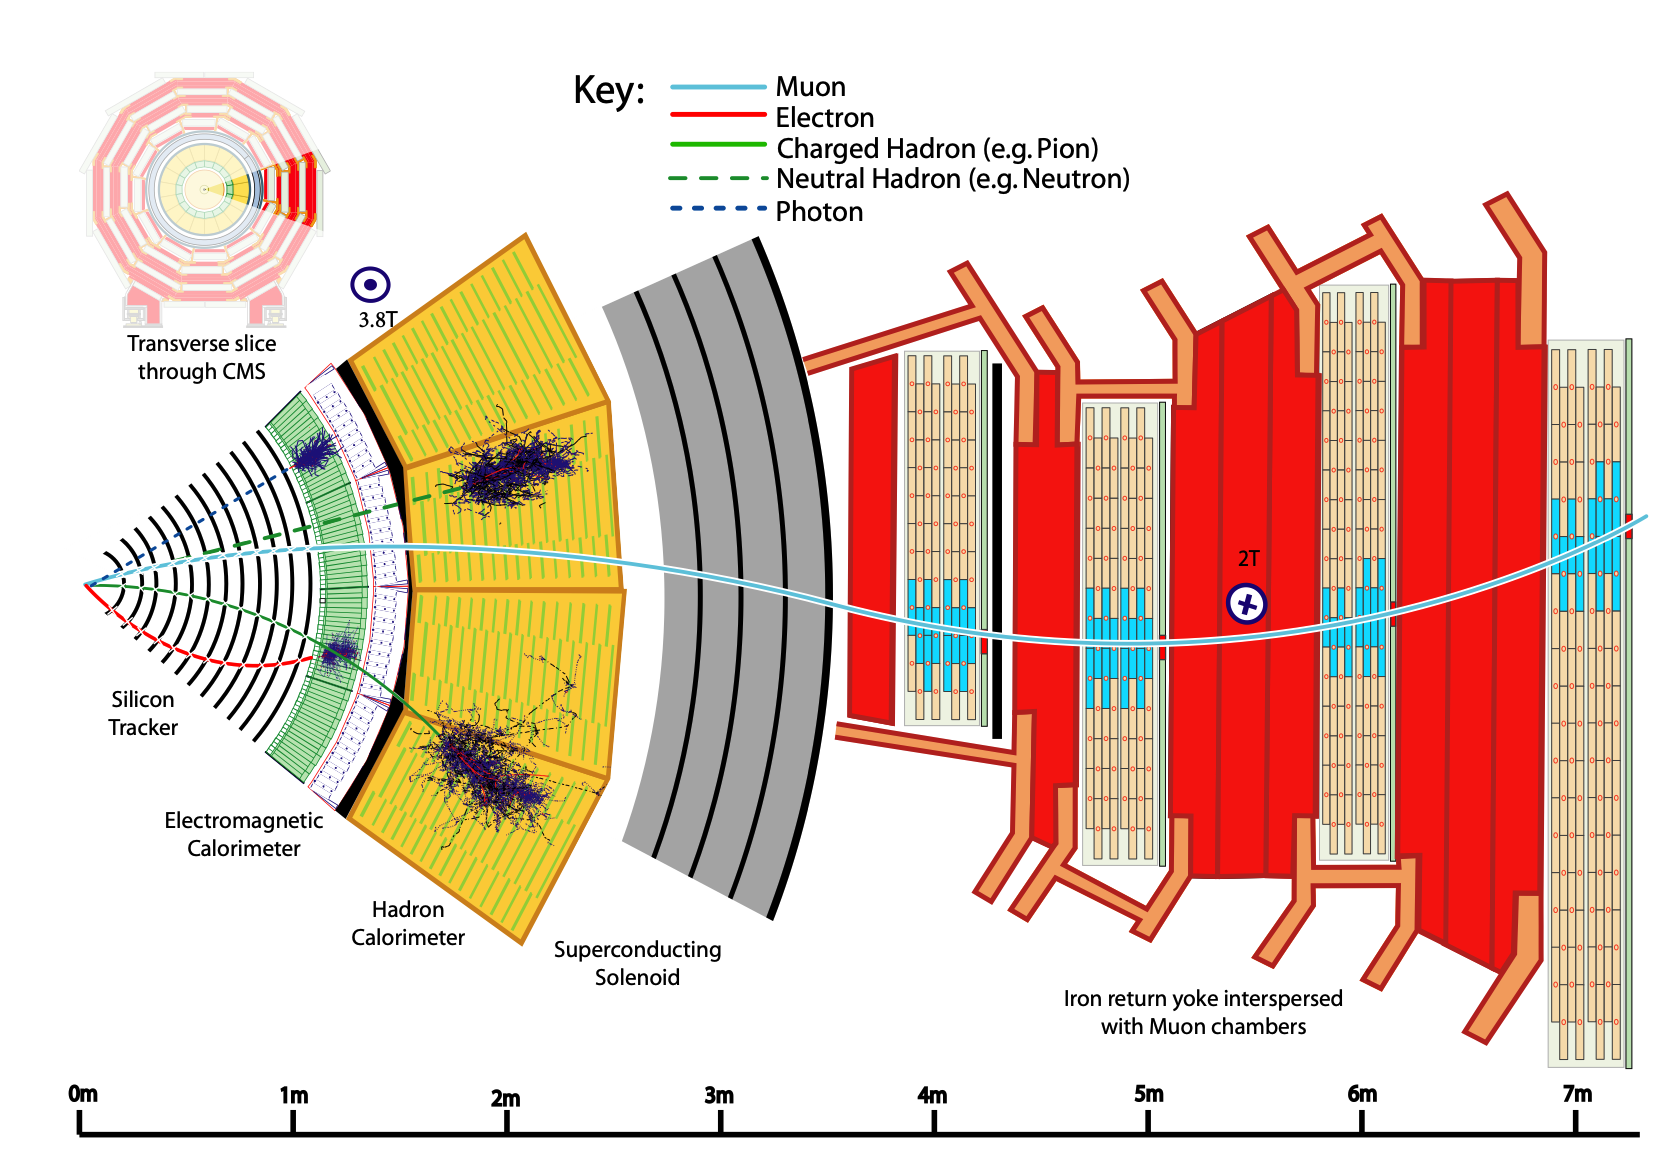
\includegraphics[width=11cm]{figures/ch-2-cern-cms/sketch-cms-particle-interactions.png}
    \caption[Sketch of particle trajectories of muons, electrons, charged and neutral hadrons, and photons in a transverse cross-section of the CMS detector.]{Sketch of particle trajectories of muons, electrons, charged and neutral hadrons, and photons in a transverse cross-section of the CMS detector \cite{CERN-EP-2017-110}.}
    \label{fig:sketch-cms-particle-interactions}
\end{figure}

CMS uses a right-handed coordinate system \cite{CMS-2008-JINST-3-S08004}. The origin is centered at the nominal collision point inside the experiment. The $x$ axis points towards the center of the LHC, and the $y$ axis points vertically upwards. The $z$ axis points along the beam direction. The azimuthal angle, $\phi$, is measured from the $x$ axis in the $x$-$y$ plane, and the radial coordinate in this plane is denoted by $r$. The polar angle, $\theta$, is measured from the $z$ axis. The pseudorapidity, $\eta$, is defined as $\eta = -\ln \tan(\theta/2)$. The momentum and energy transverse to the beam direction, denoted by $p_{T}$ and $E_{T}$ respectively, are computed from the $x$ and $y$ components. The momentum imbalance in the transverse plane is called the missing transverse momentum, and its magnitude is denoted by $E_{T}^{\text{miss}}$.

\section{Sub-detectors of CMS}
This section details the sub-detectors of CMS that operate to identify and precisely measure muons, electrons, photons, and jets over a large energy range. 

\subsection{Inner tracking system}

The CMS Tracker performs robust tracking and detailed vertex reconstruction in the 4 T magnetic field of the superconducting solenoidal magnet. The primary sensors used in the tracker are $p^+$ on $n$-bulk devices, which allow high voltage operation and are radiation-resistant \cite{CERN-LHCC-98-006} \cite{CERN-LHCC-2017-009-tracker-phase2-tdr}. The active envelope of the CMS Tracker extends to a radius of 115 cm, over a length of approximately 270 cm on each side of the interaction point \cite{CERN-LHCC-98-006}.
Charged particles in the region $|\eta| \lesssim 1.6$ benefit from the full momentum measurement precision. In this region, a charged particle with $p_T$ of 1000\GeV has a sagitta of $\sim 195$ $\mu$m. The Tracker acceptance extends further to $|\eta| = 2.5$, with a reduced radius of approximately 50 cm.

The high magnetic field of CMS causes low $p_{T}$ charged particles to travel in helical trajectories with small radii. The majority of events contain particles with a steeply falling $p_{T}$ spectrum, resulting in a track density which rapidly decreases at higher radii. 

A schematic view of the current Phase-1 CMS tracker \cite{CMS-TDR-011-pixel}, including the pixel detector, is shown in Fig. \ref{fig:phase-1-tdr-tracker-schematic}. The Phase-1 pixel detector consists of three barrel layers (BPIX) at radii of 4.4 cm, 7.3 cm, and 10.2 cm, and two forward/backward disks (FPIX) at longitudinal positions of $\pm$ 34.5 cm and $\pm$ 46.5 cm, and extending in radius from about 6 cm to 15 cm. These pixelated detectors produce 3D measurements along the paths of charged particles with single hit resolutions between 10-20 $\mu$m. 


\begin{figure}[ht]
    \centering
    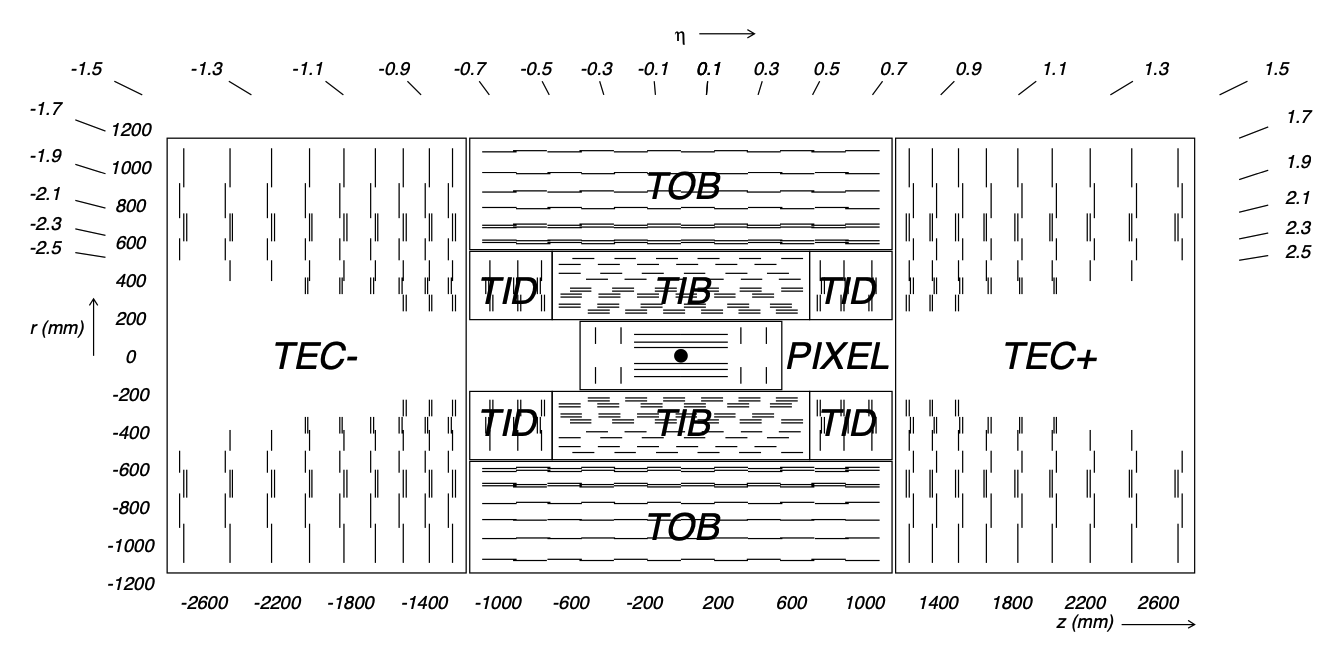
\includegraphics[width=11cm]{figures/ch-2-cern-cms/phase-1-tdr-tracker-schematic.png}
    \caption[Cross section of the current Phase-1 CMS tracker.]{Cross section of the current Phase-1 CMS tracker \cite{CMS-TDR-011-pixel}. Each line represents a detector module. Double lines indicate back-to-back modules which deliver two-dimensional (stereo) hits in the strip tracker.}
    \label{fig:phase-1-tdr-tracker-schematic}
\end{figure}

After the pixel and on their way out of the tracker, particles pass through the silicon strip tracker which reaches out to a radius of 130 cm (Fig. \ref{fig:phase-1-tdr-tracker-schematic}). The sensor elements in the strip tracker are single-sided $p$-on-$n$ type silicon micro-strip sensors \cite{CMS-2008-JINST-3-S08004}. The silicon strip detector consists of four inner barrel (TIB) layers assembled in shells, with two inner endcaps (TID), each composed of three small discs. The outer barrel (TOB) consists of six concentric layers. Two endcaps (TEC) close off the tracker on either end. 


\subsection{ECAL} 
The electromagnetic calorimeter (ECAL) of CMS measures electromagnetic energy deposits with high granularity. One of the driving criteria in the design was the capability of detecting the Standard Model Higgs boson decay to two photons (in fact, the channel in which the 125\GeV Higgs boson was discovered at CMS). 
ECAL is a hermetic homogeneous calorimeter comprised of 61,200 lead tungstate (PbWO$_4$) crystals mounted in the central barrel, with 7,324 crystals in each of the two endcaps \cite{CMS-2008-JINST-3-S08004}. A preshower detector is located in front of the endcap crystals. Avalanche photodiodes (APDs) are used as photodetectors in the barrel and vacuum phototriodes (VPTs) in the endcaps. 

The design of the ECAL is driven by the behaviour of high-energy electrons, which predominantly lose energy in matter via bremsstrahlung, and high-energy photons by $e^+ e^-$ pair production. The characteristic amount of matter traversed for these interactions is the radiation length $X^0$, usually measured in units of g cm$^-2$. The radiation length is also the mean distance over which a high-energy electron loses all but $1/e$ of its energy via bremsstrahlung \cite{workman_review_2022}. Thus high granularity in $\eta$ and $\phi$, and the length of the ECAL crystals, is designed to capture the shower of $e/\gamma$ produced by electrons and photons.

The barrel part of the ECAL (EB) covers the pseudorapidity range $|\eta| < 1.479$ \cite{CMS-2008-JINST-3-S08004}. The barrel granularity is 360-fold in $\phi$ and ($2 \times 85$)-fold in $\eta$. The crystal cross-section corresponds to approximately $0.0174 \times 0.0174$ in $\eta-\phi$ or $22 \times 22$ mm$^2$ at the front face of the crystal, and $26 \times 26$ mm$^2$ at the rear face. The crystal length is 230 mm, corresponding to 25.8 $X_0$.

The ECAL read-out acquires the signals of the photodetectors  \cite{CMS-2008-JINST-3-S08004}. At each bunch crossing, digital sums representing the energy deposit in a trigger tower, comprising $5 \times 5$ crystals in $\eta \times \phi$, are generated and sent to the Level-1 trigger system (detailed in Section \ref{section:phase-1-l1-trigger}).

\subsection{HCAL}
The hadronic calorimeter (HCAL) of CMS measures hadronic energy, which is key to characterizing the presence of apparent missing transverse energy which could arise from hadron jets and neutrinos or exotic particles \cite{CMS-2008-JINST-3-S08004}. A schematic of the components of HCAL are shown in Fig. \ref{fig:phase-1-HCAL-schematic}. The HCAL barrel (HB) and endcaps (HE) are located outside of the tracker and the ECAL, spanning a radius of 1.77 m (outer extent of ECAL) up to 2.95 m (inner extent of the magnet coil). An outer hadron calorimeter (HO) is placed outside the solenoid to complement the barrel calorimeter. Beyond $|\eta| = 3$, the forward hadron calorimeter (HF) at 11.2 m from the interaction point extend the pseudorapidity coverage to $|\eta| = 5.2$.

\begin{figure}[ht]
    \centering
    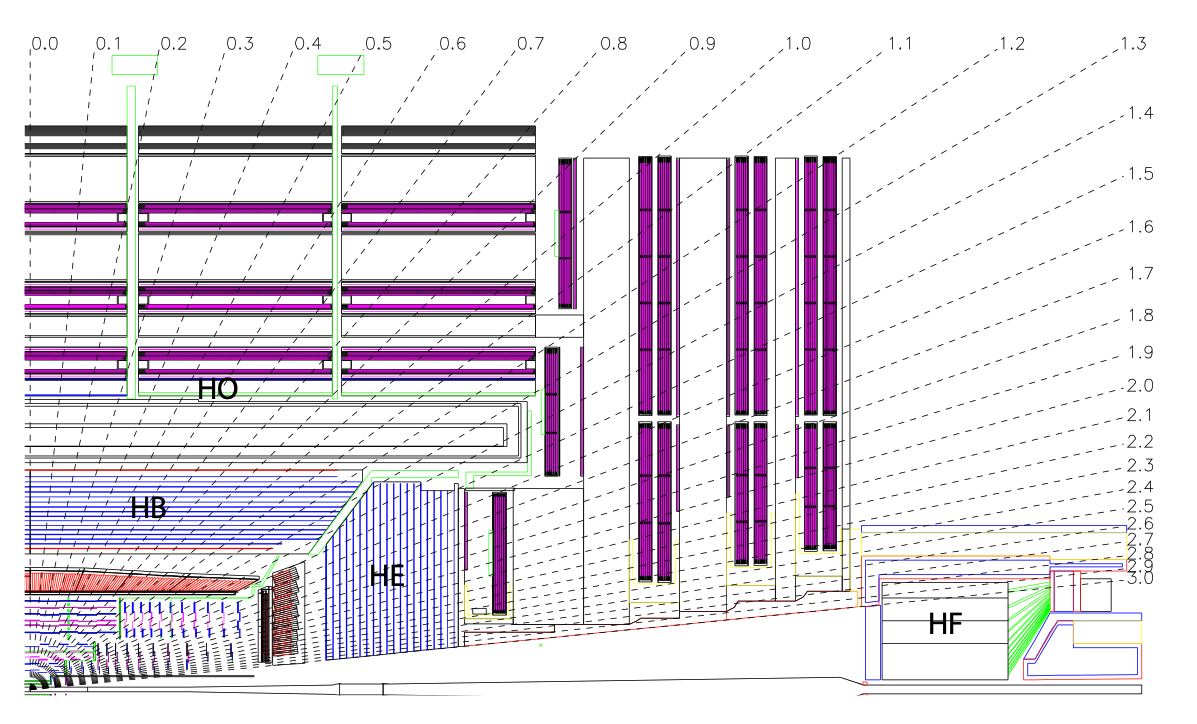
\includegraphics[width=11cm]{figures/ch-2-cern-cms/phase-1-HCAL-schematic.png}
    \caption[Longitudinal view of the CMS detector showing the hadron calorimeter barrel (HB), endcap (HE), outer (HO), and forward (HF) calorimeters.]{Longitudinal view of the CMS detector showing the hadron calorimeter barrel (HB), endcap (HE), outer (HO), and forward (HF) calorimeters from \cite{CMS-2008-JINST-3-S08004}.}
    \label{fig:phase-1-HCAL-schematic}
\end{figure}

The HB is a sampling calorimeter covering the pseudorapidity range $|\eta| < 1.3$ \cite{CMS-2008-JINST-3-S08004}. It consists of 36 identical azimuthal wedges which form two half-barrels (HB+ and HB-), with a segmentation of $(\Delta \eta, \Delta \phi) = (0.087, 0.087)$. The HE covers pseudorapidity $1.3 < |\eta| < 3$. The HB and endcap HE calorimeters are sampling calorimeters which use brass as the absorber and plastic scintillator as the active material. Light from the plastic scintillator is wavelength-shifted and captured in optic fibers which are read out by front-end electronics \cite{CMS-TDR-010-2012}. 

In the central pseudorapidity region, the combined stopping power of EB plus the HB is insufficient to contain hadron showers \cite{CMS-2008-JINST-3-S08004}. To ensure adequate sampling depth, the hadron calorimeter is extended with a tail catcher, the HO. The size and position of the tiles are designed to roughly map the layers of the HB to make towers with the same granularity of $0.087 \times 0.087$ in $\eta$ and $\phi$. HO uses the same active material as the HB and HE calorimeters, but uses the steel return yoke and magnet material of CMS as absorbers \cite{CMS-TDR-010-2012}. 


The HF is a Cherenkov calorimeter based on a steel absorber and quartz fibers which run longitudinally through the absorber and collect Cherenkov light, primarily from the electromagnetic component of showers developed in the calorimeter \cite{CMS-TDR-010-2012}. Photomultiplier tubes are used to  collect light from the quartz fibers. The HF is designed to survive in the harsh radiation conditions and high particle flux of the forward region. On average, 760\GeV per proton-proton interaction is deposited into the two forward calorimeters, compared to only 100\GeV for the rest of the detector \cite{CMS-2008-JINST-3-S08004}. Furthermore, this energy has a pronounced maximum at the highest rapidities.

\subsection{Muon detectors}
The CMS muon system is designed to have the capability of reconstructing the momentum and charge of muons over the kinematic range of the LHC, since muons are a powerful handle on signatures of interesting processes over the high background rate of the LHC \cite{CMS-2008-JINST-3-S08004}. For instance, the decay of the Standard Model Higgs boson into $ZZ$, which in turn decay to 4 leptons, can be reconstructed with high 4-particle mass resolution if all the leptons are muons, since muons are less affected than electrons by radiative losses in the tracker material. 

The muon system consists of a cylindrical barrel section and two planar endcap regions \cite{CMS-2008-JINST-3-S08004}. The barrel muon detector consists of drift tube (DT) chambers covering the pseudorapidity region $|\eta| < 1.2$ (Fig. \ref{fig:phase-1-muon-barrel-DT-schematic}). The DTs can be used as tracking detectors due to the barrel region's characteristic low neutron-induced backgrounds, low muon rate, and relatively uniform 4T magnetic field contained in the steel yoke. 

\begin{figure}[ht]
    \centering
    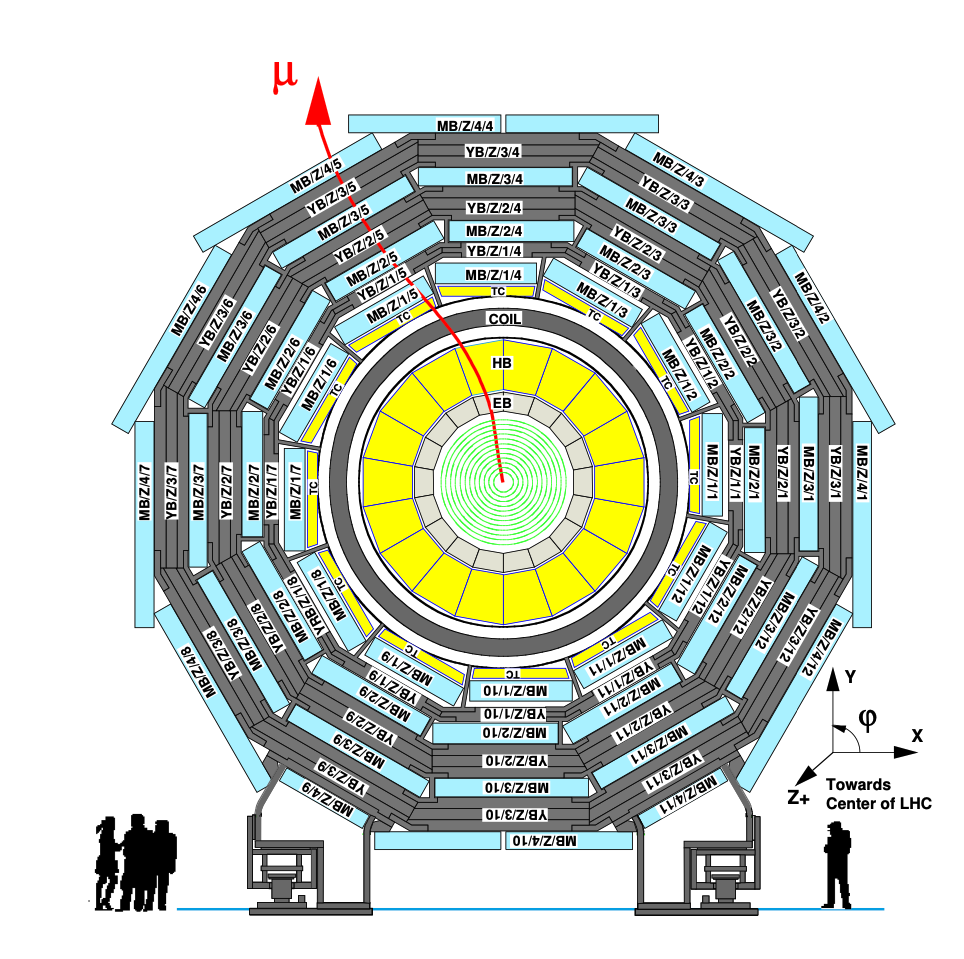
\includegraphics[width=11cm]{figures/ch-2-cern-cms/phase-1-muon-barrel-DT-schematic.png}
    \caption[Layout of the CMS barrel muon drift tube (DT) chambers in one of the five wheels.]{Layout of the CMS barrel muon drift tube (DT) chambers in one of the five wheels from \cite{CMS-2008-JINST-3-S08004}. The DTs are organized in 12 sectors of the yoke barrel (YB). In each of the 12 sectors of the yoke, there are 4 muon chambers per wheel (MB1, MB2, MB3, and MB4).}
    \label{fig:phase-1-muon-barrel-DT-schematic}
\end{figure}

In the two endcap regions, the muon rates and background levels are high and the magnetic field is large and non-uniform \cite{CMS-2008-JINST-3-S08004}. Here, the muon system uses cathode strip chambers (CSCs) to identify muons between $0.9 < |\eta| < 2.4$. The cathode strips of each chamber run radially outwards and provide a precision measurement in the $r-\phi$ bending plane. The anode wires run approximately perpendicular to the strips and are read out in order to measure $\eta$ and the beam-crossing time of a muon. 

% 2008 JINST 3 S08004, page 164
In addition to the DT and CSC, a dedicated trigger system consisting of resistive plate chambers (RPCs) in the barrel and endcap regions provide a fast, independent, and highly-segmented trigger with a sharp $p_T$ threshold over a large portion of the pseudorapidity range ($|\eta| < 1.6$) of the muon system \cite{CMS-2008-JINST-3-S08004}. RPCs have good time resolution but coarser position resolution compared to the DTs or CSCs. The RPCs also play a role in resolving ambiguities in reconstructing tracks from multiple hits in a chamber. 

\subsection{The Level-1 Trigger}
\label{section:phase-1-l1-trigger}
The design performance of the LHC corresponds to an instantaneous luminosity of $10^{34}$ cm$^{-2}$ s$^{-1}$ with a 25 ns bunch crossing rate, giving an average pile-up (number of simultaneous events) of 25 per bunch crossing \cite{CMS-TDR-012}. The large number of minimum bias events per bunch crossing, combined with the small cross-sections of possible physics discovery signatures, necessitates a sophisticated event selection system for filtering this large event rate, as it is impossible to save all events. This data filtering system is implemented by CMS in two stages. The first stage is the Level-1 (L1) Trigger, which is deployed in custom electronic hardware systems and is responsible for reducing the event rate to around 100 kHz. The second stage is the High-Level Trigger (HLT) which is described in Section \ref{section:phase-1-high-level-trigger}. This section describes the Phase-1 configuration of the Level-1 Trigger.


The L1 Trigger data flow of Phase-1 is shown in Fig. \ref{fig:phase-1-level-1-trigger-dataflow} \cite{CMS-TDR-012}, with organization into the L1 calorimeter trigger, the L1 muon trigger, and the L1 global trigger. 

\begin{figure}[ht]
    \centering
    \includegraphics[width=11cm]{figures/ch-2-cern-cms/phase-1-level-1-trigger-dataflow.png}
    \caption[Dataflow for the Phase-1 Level-1 Trigger.]{Dataflow for the Phase-1 Level-1 Trigger \cite{CMS-TDR-012}, which is implemented in custom hardware and is responsible for reducing the event rate from the LHC bunch crossing frequency of 400 MHz (bunch crossings every 25 ns) to a maximum rate of 100 kHz. In Phase-1, the Level-1 Trigger has access to information from the calorimeter and muon detectors.}
    \label{fig:phase-1-level-1-trigger-dataflow}
\end{figure}

The L1 calorimeter trigger begins with trigger tower energy sums formed by the ECAL, HCAL, and HF Trigger Primitive Generator (TPG) circuits from the individual calorimeter cell energies. In the original configuration, the ECAL energies were accompanied by a bit indicating the transverse extent of the electromagnetic energy deposits, and the HCAL energies were accompanied by a bit indicating the presence of minimum ionizing energy \cite{CERN-LHCC-2000-038}. Between Long Shutdowns 1 and 2 (LS1 and LS2), HF was upgraded to provide finer granularity information to the trigger, and the HCAL barrel and endcap front-end electronics were upgraded to provide high-precision timing information and depth segmentation information. 

In the original design of the L1 calorimeter trigger, the trigger primitives are processed by the Regional Calorimeter Trigger (RCT, upgraded to Calo Layer 1 after LS2) which finds isolated and non-isolated electron/photon candidates \cite{CMS-TDR-012}. At this stage, electrons/photons candidates are treated together since they cannot be definitively distinguished at this stage due to lack of tracking information in the L1 trigger. The Global Calorimeter Trigger (GCT, upgraded to Calo Layer 2 after LS2) sorts further the candidate electrons/photons, finds jets (classified as central, forward, and tau) using the $E_T$ sums and performs calibration of the clustered jet energies, and calculates global quantities such as missing $E_T$. It sends the top four candidates of each type to the global trigger (GT) \cite{CMS-TDR-012}.

Each of the L1 muon triggers has its own trigger logic \cite{CERN-LHCC-2000-038}. The RPC strips are connected to a Pattern Comparator Trigger (PACT), which forms trigger segments that are used to build tracks and calculate $p_{T}$. The RPC logic also provides some hit data to the CSC trigger system to resolve ambiguities caused by two muons in the same CSC. The CSCs form local charged tracks (LCTs) from the cathode strips, which are combined with the anode wire information. LCTs are combined into full muon tracks and assigned $p_{T}$ values. 

The Global Muon Trigger (GMT) sorts the RPC, DT, and CSC muon tracks, converts these tracks to the same $\eta$, $\phi$, and $p_{T}$ scale, and validates the muon sign \cite{CERN-LHCC-2000-038}. It improves the trigger efficiency by merging muon candidates that were detected in two complementary sub-systems (i.e. DT+RPC, or CSC+RPC). The GMT also contains logic to correlate the found muon tracks with an $\eta-\phi$ grid of quiet calorimeter towers to determine if the muons are isolated, as well as logic to remove duplicate candidates originating in the overlap regions from both DT and CSC systems. The final collection of muons are sorted based on their initial quality, correlation, and $p_{T}$, and the top four muons are sent to the Global Trigger \cite{CERN-LHCC-2000-038}. 

Information from the GCT and GT are sent to the Global Trigger (GT), which makes the Level-1 Accept (L1A) decision to either discard or accept the bunch crossing \cite{CERN-LHCC-2000-038}. This is accomplished by sorting ranked trigger objects that are accompanied by positional information in $\eta$ and $\phi$, permitting the trigger to applying criteria with thresholds that can vary based on the location of the trigger objects, and/or to require trigger objects to be close to or opposite from each other. The GT L1A decision arrives at the detector front end with a 3.8 $\mu$s latency after the interaction at a rate which is required to be less than 100 kHz, and triggers a full readout of the detector for further processing.



\subsection{The High-Level Trigger}
\label{section:phase-1-high-level-trigger}
The HLT is implemented in software running on a large computer farm of fast commercial processors \cite{CMS-TDR-022-HLT} \cite{Foudas:2008dt}. The algorithms in HLT have access to full data from all CMS sub-detectors, including the tracker, with full granularity and resolution. The HLT reconstruction software is similar to what is used offline for full CMS data analysis. As a result, the HLT can calculate quantities with a resolution comparable to the final detector resolution, compared to the L1 Trigger. The HLT performs more computationally-intensive algorithms, such as combining tau-jet candidates in the calorimeter with high-$p_T$ stubs in the tracker, to form a hadronic tau trigger. The maximum HLT input rate from the L1 Trigger is 100 kHz, and the HLT output rate is approximately 100 Hz. 

The HLT contains trigger paths, each corresponding to a dedicated trigger \cite{twiki_SoftwareGuide_HLT}.  A path consists of several steps implemented as software modules. Each HLT trigger path must be seeded by one or more L1 trigger bits: the first module always looks for a L1 seed, consisting of L1 bit(s) and L1 object(s). Each module performs a well-defined task such as unpacking (raw to digitized quantities), reconstruction of physics objects (electrons, muons, jet, missing transverse energy, etc.), making intermediate decisions that trigger more detailed reconstruction modules, and calculating the final decision for the trigger path. If an intermediate filter decision is negative, the rest of the path is not executed, and the trigger rejects the event.


\subsection{Particle reconstruction}
To build a description of the physics objects present in the particle collision, the basic elements from the detector layers (tracks and clusters of energy) are correlated to identify each particle in the final state. Measurements from different sub-detectors are combined to reconstruct the particle properties. This approach is called particle-flow (PF) reconstruction \cite{CERN-EP-2017-110}. Key to the success of the PF reconstruction is the fine spatial granularity of the detector layers. Coarse-grained detectors can cause the signals from different particles to merge, especially within jets. However, if the subdetectors are sufficiently segmented to separate individual particles, it becomes possible to produce a global event description that identifies all physics objects with high efficiencies and resolution.

\subsection{Data storage and computational infrastructure}

The LHC generates over 15 petabytes (15 million gigabytes) of data every year, necessitating a flexible computing system that can be accessed by researchers working at the four main LHC experiments: ALICE, ATLAS, CMS, and LHCb. The Worldwide LHC Computing Grid (WLCG) \cite{computing-Worldwide:1997398} is a global collaboration of computer centers that links thousands of computers and storage systems in over 170 centers across 41 countries. These centers are arranged in ``tiers'', and provide near real-time access to users processing, analyzing, and storing LHC data. One of the final stages of data analysis at LHC experiments is large-scale data processing taking place over distributing computing, for instance, with the use of Condor \cite{condor-article}, a distributed, scalable, flexible batch processing system which accepts a computing job, allocates a resource to it, executes it, and returns the result back to a user transparently. 
 


\chapter{The CMS Phase-1 Level-1 Trigger}

\section{The Phase-1 Level-1 Trigger}
\label{section:phase-1-l1-trigger}
The design performance of the LHC corresponds to an instantaneous luminosity of $10^{34}$ cm$^{-2}$ s$^{-1}$ with a 25 ns bunch crossing rate, giving an average pile-up (number of simultaneous events) of 25 per bunch crossing \cite{CMS-TDR-012}. The large number of minimum bias events per bunch crossing, combined with the small cross-sections of possible physics discovery signatures, necessitates a sophisticated event selection system for filtering this large event rate, as it is impossible to save all events. This data filtering system is implemented by CMS in two stages. The first stage is the Level-1 (L1) Trigger, which is deployed in custom electronic hardware systems and is responsible for reducing the event rate to around 100 kHz. The second stage is the High-Level Trigger (HLT) which is described in Section \ref{section:phase-1-high-level-trigger}. This section describes the Phase-1 configuration of the Level-1 Trigger.


The L1 Trigger data flow of Phase-1 is shown in Fig. \ref{fig:phase-1-level-1-trigger-dataflow} \cite{CMS-TDR-012}, with organization into the L1 calorimeter trigger, the L1 muon trigger, and the L1 global trigger. 

\begin{figure}[ht]
    \centering
    \includegraphics[width=11cm]{figures/ch-3-phase1-l1-trigger/phase-1-level-1-trigger-dataflow.png}
    \caption[Dataflow for the Phase-1 Level-1 Trigger.]{Dataflow for the Phase-1 Level-1 Trigger \cite{CMS-TDR-012}, which is implemented in custom hardware and is responsible for reducing the event rate from the LHC bunch crossing frequency of 400 MHz (bunch crossings every 25 ns) to a maximum rate of 100 kHz. In Phase-1, the Level-1 Trigger has access to information from the calorimeter and muon detectors.}
    \label{fig:phase-1-level-1-trigger-dataflow}
\end{figure}

The L1 calorimeter trigger begins with trigger tower energy sums formed by the ECAL, HCAL, and HF Trigger Primitive Generator (TPG) circuits from the individual calorimeter cell energies. In the original configuration, the ECAL energies were accompanied by a bit indicating the transverse extent of the electromagnetic energy deposits, and the HCAL energies were accompanied by a bit indicating the presence of minimum ionizing energy \cite{CERN-LHCC-2000-038}. Between Long Shutdowns 1 and 2 (LS1 and LS2), HF was upgraded to provide finer granularity information to the trigger, and the HCAL barrel and endcap front-end electronics were upgraded to provide high-precision timing information and depth segmentation information. 

In the original design of the L1 calorimeter trigger, the trigger primitives are processed by the Regional Calorimeter Trigger (RCT, upgraded to Calo Layer 1 after LS2) which finds isolated and non-isolated electron/photon candidates \cite{CMS-TDR-012}. At this stage, electrons/photons candidates are treated together since they cannot be definitively distinguished at this stage due to lack of tracking information in the L1 trigger. The Global Calorimeter Trigger (GCT, upgraded to Calo Layer 2 after LS2) sorts further the candidate electrons/photons, finds jets (classified as central, forward, and tau) using the $E_T$ sums and performs calibration of the clustered jet energies, and calculates global quantities such as missing $E_T$. It sends the top four candidates of each type to the global trigger (GT) \cite{CMS-TDR-012}.

Each of the L1 muon triggers has its own trigger logic \cite{CERN-LHCC-2000-038}. The RPC strips are connected to a Pattern Comparator Trigger (PACT), which forms trigger segments that are used to build tracks and calculate $p_{T}$. The RPC logic also provides some hit data to the CSC trigger system to resolve ambiguities caused by two muons in the same CSC. The CSCs form local charged tracks (LCTs) from the cathode strips, which are combined with the anode wire information. LCTs are combined into full muon tracks and assigned $p_{T}$ values. 

The Global Muon Trigger (GMT) sorts the RPC, DT, and CSC muon tracks, converts these tracks to the same $\eta$, $\phi$, and $p_{T}$ scale, and validates the muon sign \cite{CERN-LHCC-2000-038}. It improves the trigger efficiency by merging muon candidates that were detected in two complementary sub-systems (i.e. DT+RPC, or CSC+RPC). The GMT also contains logic to correlate the found muon tracks with an $\eta-\phi$ grid of quiet calorimeter towers to determine if the muons are isolated, as well as logic to remove duplicate candidates originating in the overlap regions from both DT and CSC systems. The final collection of muons are sorted based on their initial quality, correlation, and $p_{T}$, and the top four muons are sent to the Global Trigger \cite{CERN-LHCC-2000-038}. 

Information from the GCT and GT are sent to the Global Trigger (GT), which makes the Level-1 Accept (L1A) decision to either discard or accept the bunch crossing \cite{CERN-LHCC-2000-038}. This is accomplished by sorting ranked trigger objects that are accompanied by positional information in $\eta$ and $\phi$, permitting the trigger to applying criteria with thresholds that can vary based on the location of the trigger objects, and/or to require trigger objects to be close to or opposite from each other. The GT L1A decision arrives at the detector front end with a 3.8 $\mu$s latency after the interaction at a rate which is required to be less than 100 kHz, and triggers a full readout of the detector for further processing.



\chapter{The Phase-2 Upgrade of CMS}
\label{chapter:phase-2-upgrade-cms}
\section{High-Luminosity LHC and CMS}
In order to sustain and extend the LHC's physics discovery program and maintain operability for a decade or more, the LHC is undergoing a major upgrade to the  High-Luminosity LHC (HL-LHC). In its final configuration, the HL-LHC will deliver a peak luminosity of $7.5 \times 10^{34}$ cm$^{-2}$ s$^{-1}$, potentially leading to total integrated luminosity of 4000 fb$^{-1}$ after ten years of operations, scheduled to begin in 2027 \cite{CMS-TDR-021}. This integrated luminosity is about ten times the predicted luminosity reach of the LHC in its initial configuration. To maximize the discovery potential of this unprecedented amount of data, the CMS detector is undergoing Phase-2 upgrades in order to perform high-precision measurements and searches for physics beyond the Standard Model in the intense running conditions of the HL-LHC.

\section{The Phase-2 Level-1 Trigger}
To achieve the goals of the HL-LHC program and to ensure the collection of information-rich datasets in the HL-LHC, the Phase-2 upgrade of the CMS Level-1 Trigger \cite{CMS-TDR-021} must be upgraded in conjunction with the CMS sub-detectors and their readouts, to maintain physics selectivity. The HL-LHC will produce an intense hadronic environment corresponding to 200 simultaneous collisions per beam crossing, necessitating comprehensive upgrades of the trigger system outlined below.

To profit from the extended coverage and increased granularity of the upgraded CMS detector, the latency of the L1 trigger system (time available to produce a L1 Accept signal) will be increased significantly from 3.8 $\mu$s to 12.5 $\mu$s, with an increased maximum output bandwidth of 750 kHz \cite{CMS-TDR-021}. With the increased latency, in addition to information from calorimeters and muon detectors (as in the Phase-1 system), information from the new tracker and high-granularity endcap calorimeter can also be included at L1 for the first time. This is illustrated in the functional diagram of the architecture of the Phase-2 trigger system in Fig. \ref{fig:phase-2-l1-architecture}. 

\begin{figure}[ht]
    \centering
    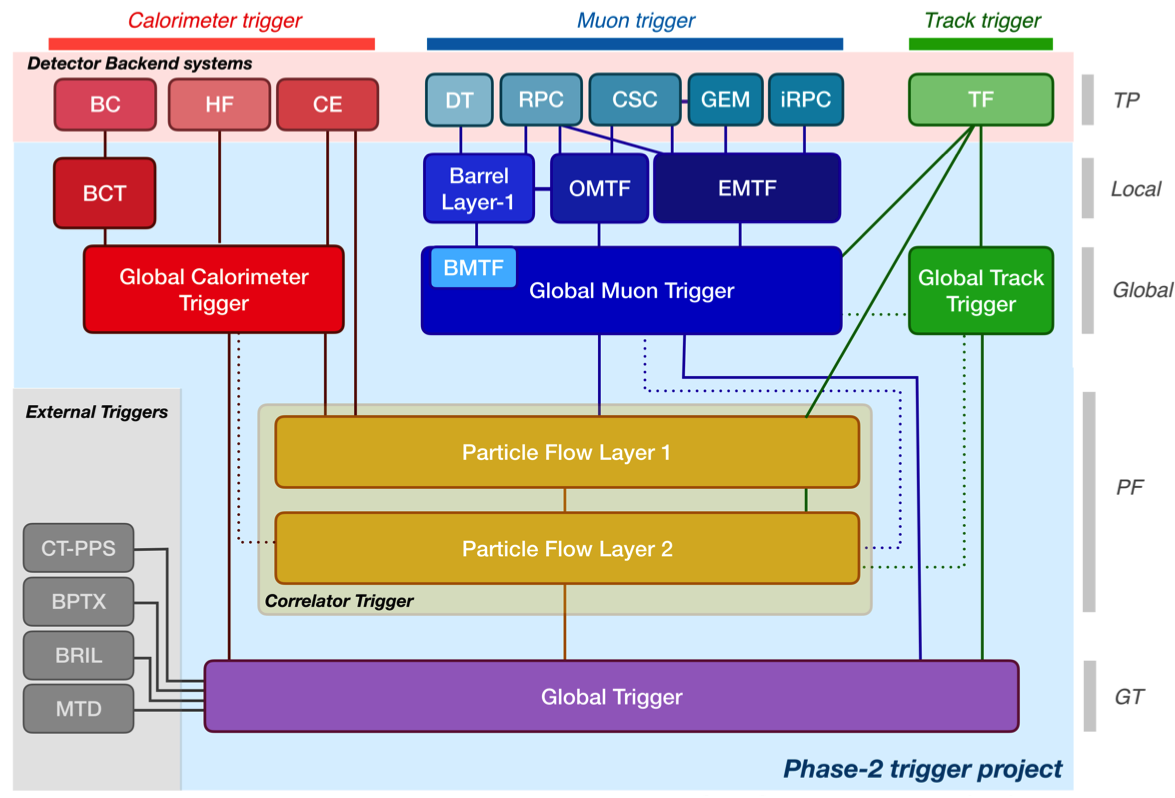
\includegraphics[width=15cm]{figures/ch-4-phase2/phase-2-l1-architecture.png}
    \caption[Functional diagram of the CMS L1 Phase-2 upgraded trigger design.]{Functional diagram of the CMS L1 Phase-2 upgraded trigger design \cite{CMS-TDR-021}, showing the four trigger paths: calorimeter, muon, track, and Particle Flow. For the first time, tracking information will be available as early as the L1 Trigger.}
    \label{fig:phase-2-l1-architecture}
\end{figure}

The key feature of the Phase-2 L1 Trigger is the introduction of a correlator layer, where algorithms produce higher-level trigger objects by combining information from sub-detectors, with a selectivity approaching that of offline reconstruction in the HLT \cite{CMS-TDR-021}. Four independent data processing paths (grouped together in Fig. \ref{fig:phase-2-l1-architecture}) are implemented: tracking, calorimetry, muon systems, and particle-flow techniques:
\begin{itemize}
    \item \textbf{Calorimeter Trigger path:} (\textit{red}, Fig. \ref{fig:phase-2-l1-architecture}) A barrel calorimeter trigger (BCT) and the HGCAL backend are used to produce high-granularity information from the calorimeters to produce high-resolution clusters and identification variables used for later processing. Outputs from the BCT, HGCAL, and the HF are sent to a global calorimeter trigger (GCT), where calorimeter-only objects such as $e/\gamma$ candidates, hadronically decaying tau lepton candidates, jets, and energy sums are built.
    \item \textbf{Track Trigger path:} (\textit{green}, Fig. \ref{fig:phase-2-l1-architecture}) Tracks from the Outer Tracker are reconstructed in the track finder (TF) processors as part of the detector backend. A global track trigger (GTT) will reconstruct the primary vertices of the event, along with tracker-only based objects, such as jets and missing transverse momentum.
    \item \textbf{Muon Trigger path:} (\textit{blue}, Fig. \ref{fig:phase-2-l1-architecture}) Trigger primitives are processed by muon track finder algorithms, again separated into the barrel (barrel muon track finder, BMTF), overlap (overlap muon track finder, OMTF), and endcap (endcap muon track finder, EMTF). Standalone muons and stubs containing information such as position, bend angle, and timing, as well as L1 tracks, are sent to the global muon trigger (GMT).
    \item \textbf{Particle-Flow Trigger path:} (\textit{yellow}, Fig. \ref{fig:phase-2-l1-architecture}) The correlator trigger (CT) aims to approach the performance of offline Particle Flow, and is implemented in two layers. ``Layer-1'' produces the particle-flow candidates from matching calorimeter clusters and tracks. ``Layer 2'' builds and sorts final trigger objects and applies additional identification and isolation criteria.
\end{itemize}

The outputs from the above trigger paths are combined in the Global Trigger (GT) (\textit{purple}, Fig. \ref{fig:phase-2-l1-architecture}), which calculates the final trigger decision (Level-1 Accept), transmitting it to the Trigger Control and Distribution System (TCDS), which distributes it to the detector backend systems, initiating the readout to the DAQ. The GT also provides the interface to external triggers (\textit{grey}, Fig. \ref{fig:phase-2-l1-architecture}), such as triggers for the precision proton spectrometer (PPS), beam position and timing monitors (BPTX), and luminosity and beam monitoring (BRIL) detectors \cite{CMS-TDR-021}. The design of the Phase-2 Level-1 Trigger allows for future inclusion of triggering information, for instance information about minimum ionizing particles (MIPs) from the MIP Timing Detector (MTD) \cite{CERN-LHCC-2017-027}.

\section{Standalone Barrel Calorimeter electron/photon reconstruction}
\begin{figure}[ht]
    \centering
    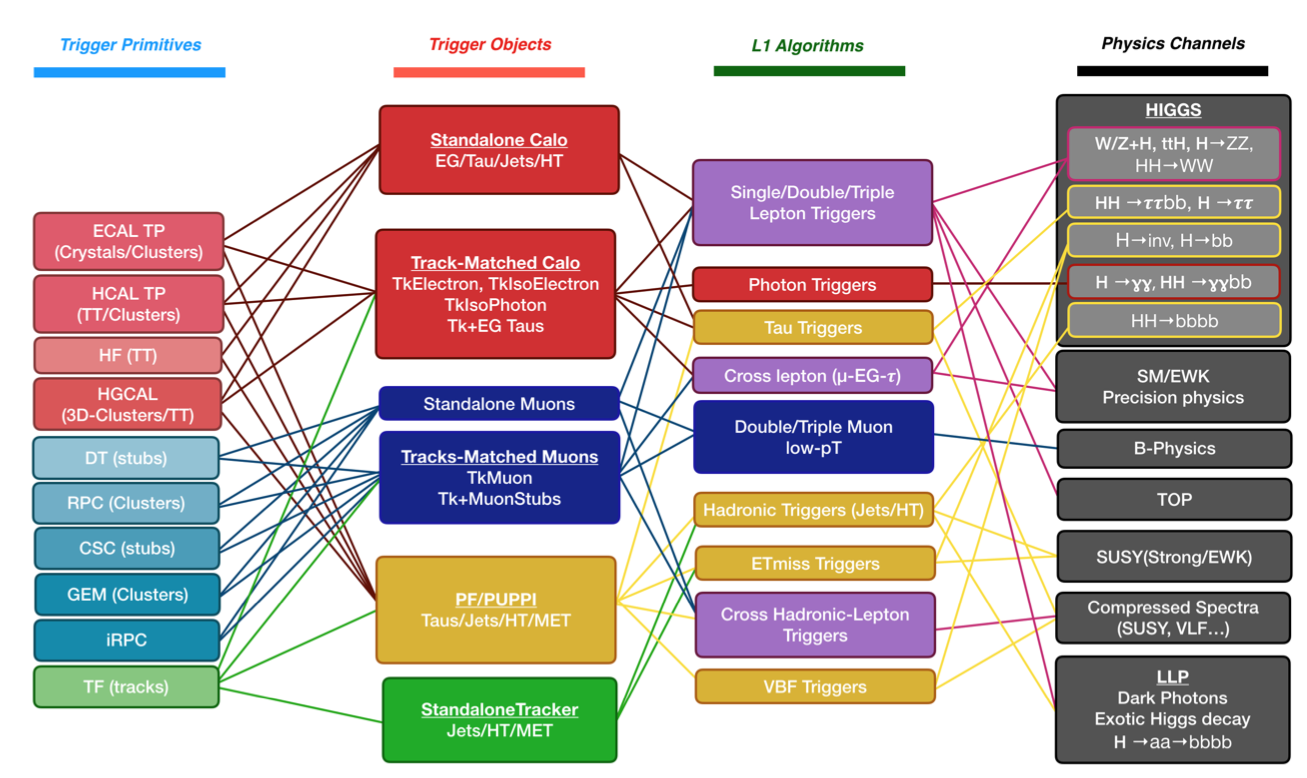
\includegraphics[width=15cm]{figures/ch-4-phase2/phase-2-summary-trigger-TP-algo-physics.png}
    \caption[Summary of the links between the trigger primitives, the trigger objects, the Level-1 algorithms, and the physics channels in the Phase-2 menu.]{Summary of the links between the trigger primitives (\textit{first column}), the trigger objects (\textit{second column}), the Level-1 algorithms used in the menu (\textit{3rd column}), and the physics channels (\textit{4th column}), from \cite{CMS-TDR-021}, where a full description of the Phase-2 L1 algorithms can be found. This work focuses on developments for the Standalone Calorimeter electron and photon ("EG") reconstruction algorithm.}
    \label{fig:phase-2-summary-trigger-TP-algo-physics}
\end{figure}

The reconstruction and identification of electrons and photons ($e/\gamma$) begin with the trigger primitives of the barrel ECAL and HCAL detectors and endcap HGCAL calorimeters, covering the pseudorapidity region $|\eta| < 3$. The barrel and endcap regions of the detector are intrinsically different enough to warrant different approaches to $e/\gamma$ reconstruction. This work focuses on the Standalone Calorimeter $e/\gamma$ reconstruction taking place in the barrel (Fig. \ref{fig:phase-2-summary-trigger-TP-algo-physics}).

\subsection{Phase-2 geometry of the ECAL Barrel trigger}
\label{section:phase-2-ECAL-barrel-geometry}
% https://cds.cern.ch/record/2714892/files/CMS-TDR-021.pdf  
% Section 2.2.1, on page 36-37
In Phase-2, the upgrade of both on-detector and off-detector electronics for the barrel calorimeters trigger primitive generator (TPG) will stream single crystal data from the on-detector to the backend electronics, in contrast to the lower-granularity output of the Phase-1 ECAL TPG that is restricted to providing trigger tower sums of $5 \times 5$ crystals \cite{CMS-TDR-021}. 
A schematic representation of the geometry of the ECAL barrel in the Regional Calorimeter Trigger (RCT) is shown in Fig. \ref{fig:phase-2-rct-cards-schematic}. The barrel is spanned by 36 RCT cards, each spanning $17 \times 4$ towers in $\eta \times \phi$. Each RCT card is subdivided into five ``regions'' as shown in Fig. \ref{fig:phase-2-one-rct-card-schematic}. After initial clustering and processing, the outputs of the RCT card are sent to the Global Calorimeter (GCT) trigger, which is processed in three cards as shown in Fig. \ref{fig:phase-2-gct-cards-schematic}.

\begin{figure}[ht]
    \centering
    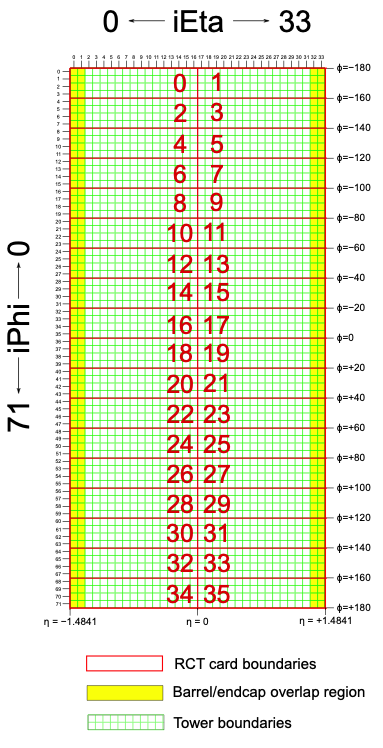
\includegraphics[width=9cm]{figures/ch-4-phase2/phase-2-rct-cards-schematic.png}
    \caption{Schematic of the geometry of the Phase-2 ECAL barrel in the Regional Calorimeter Trigger (RCT), showing the division of the barrel region into 36 Regional Calorimeter Trigger (RCT) cards (\textit{red}). Each card spans $17 \times 4$ towers in $\eta \times \phi$ (\textit{green}), and each tower is $5\times 5$ in single crystals in $\eta \times \phi$. Towers in the overlap region (\textit{shaded yellow}) are read out to both the barrel and endcap.}
    \label{fig:phase-2-rct-cards-schematic}
\end{figure}

\begin{figure}[ht]
    \centering
    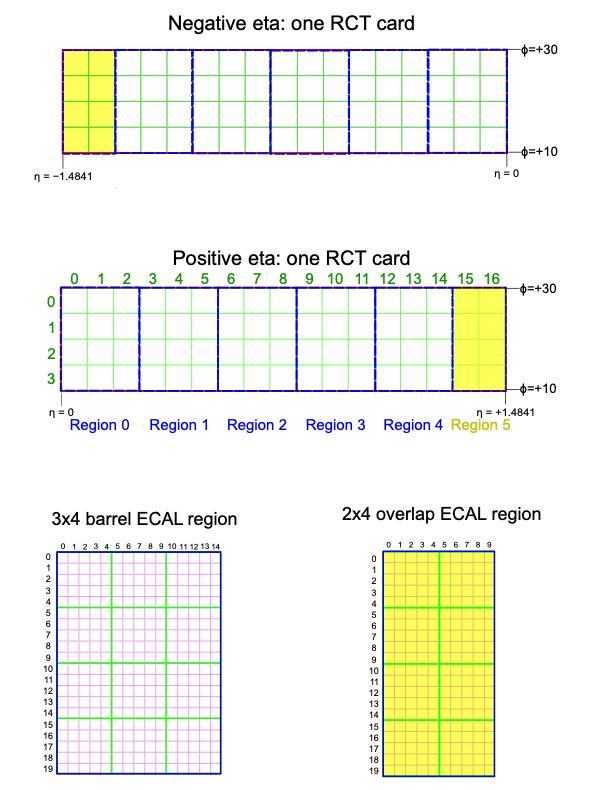
\includegraphics[width=9cm]{figures/ch-4-phase2/phase-2-one-rct-card-schematic.png}
    \caption{Schematic of two example RCT cards in the negative eta (\textit{top}) and positive eta (\textit{center}) regions of the ECAL barrel. Each RCT card is divided into five regions: four regions are of size $3 \times 4$ towers in $\eta \times \phi$ (\textit{bottom left}), and a fifth smaller overlap region of size $2 \times 4$ towers (\textit{bottom right}). Each tower is $5 \times 5$ ($\eta\times\phi$) in crystals.}
    \label{fig:phase-2-one-rct-card-schematic}
\end{figure}


\begin{figure}[ht]
    \centering
    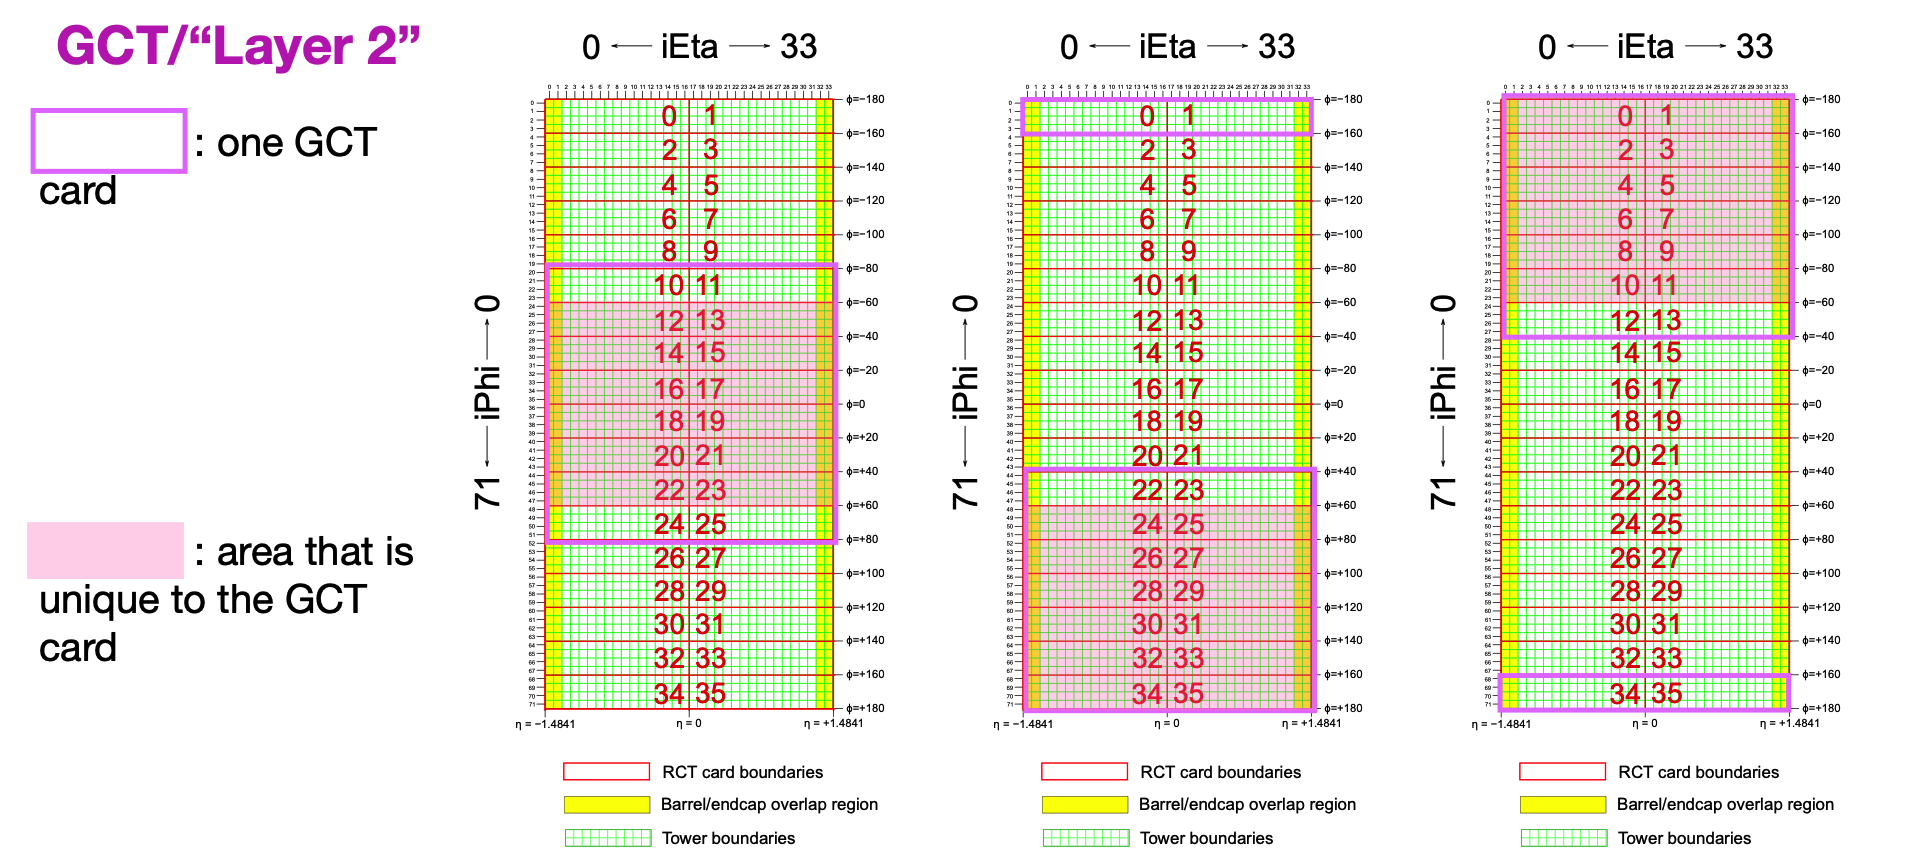
\includegraphics[width=15cm]{figures/ch-4-phase2/phase-2-gct-cards-schematic.png}
    \caption{Schematic of the Phase-2 ECAL barrel in the Global Calorimeter Trigger (GCT), which will process the outputs of the Regional Calorimeter Trigger (RCT) in three cards (\textit{magenta highlights}). Each card in the GCT processes the equivalent of sixteen RCT cards, with the center twelve being unique to that GCT card (\textit{shaded pink}), and the remaining four processed in overlap with the other GCT cards.}
    \label{fig:phase-2-gct-cards-schematic}
\end{figure}


\subsection{Phase-2 electron/photon reconstruction algorithm}
\label{section:phase-2-egamma-reconstruction-algorithm}

The standalone barrel algorithm for reconstructing and identifying electrons and photons in the Phase-2 Level-1 Trigger takes as input the digitized response of each crystal of the barrel ECAL, with a granularity $0.0175 \times 0.0175$ in $\eta \times \phi$, which is 25 times higher than the input to the Phase-1 trigger, which consisted of trigger towers with a granularity of $0.0875 \times 0.0875$. In HCAL the tower size of $0.0875 \times 0.0875$ is unchanged. The trigger algorithm is designed to closely reproduce the algorithm used in the offline reconstruction, with limitations and simplifications due to trigger latency. 

\begin{figure}[ht]
    \centering
    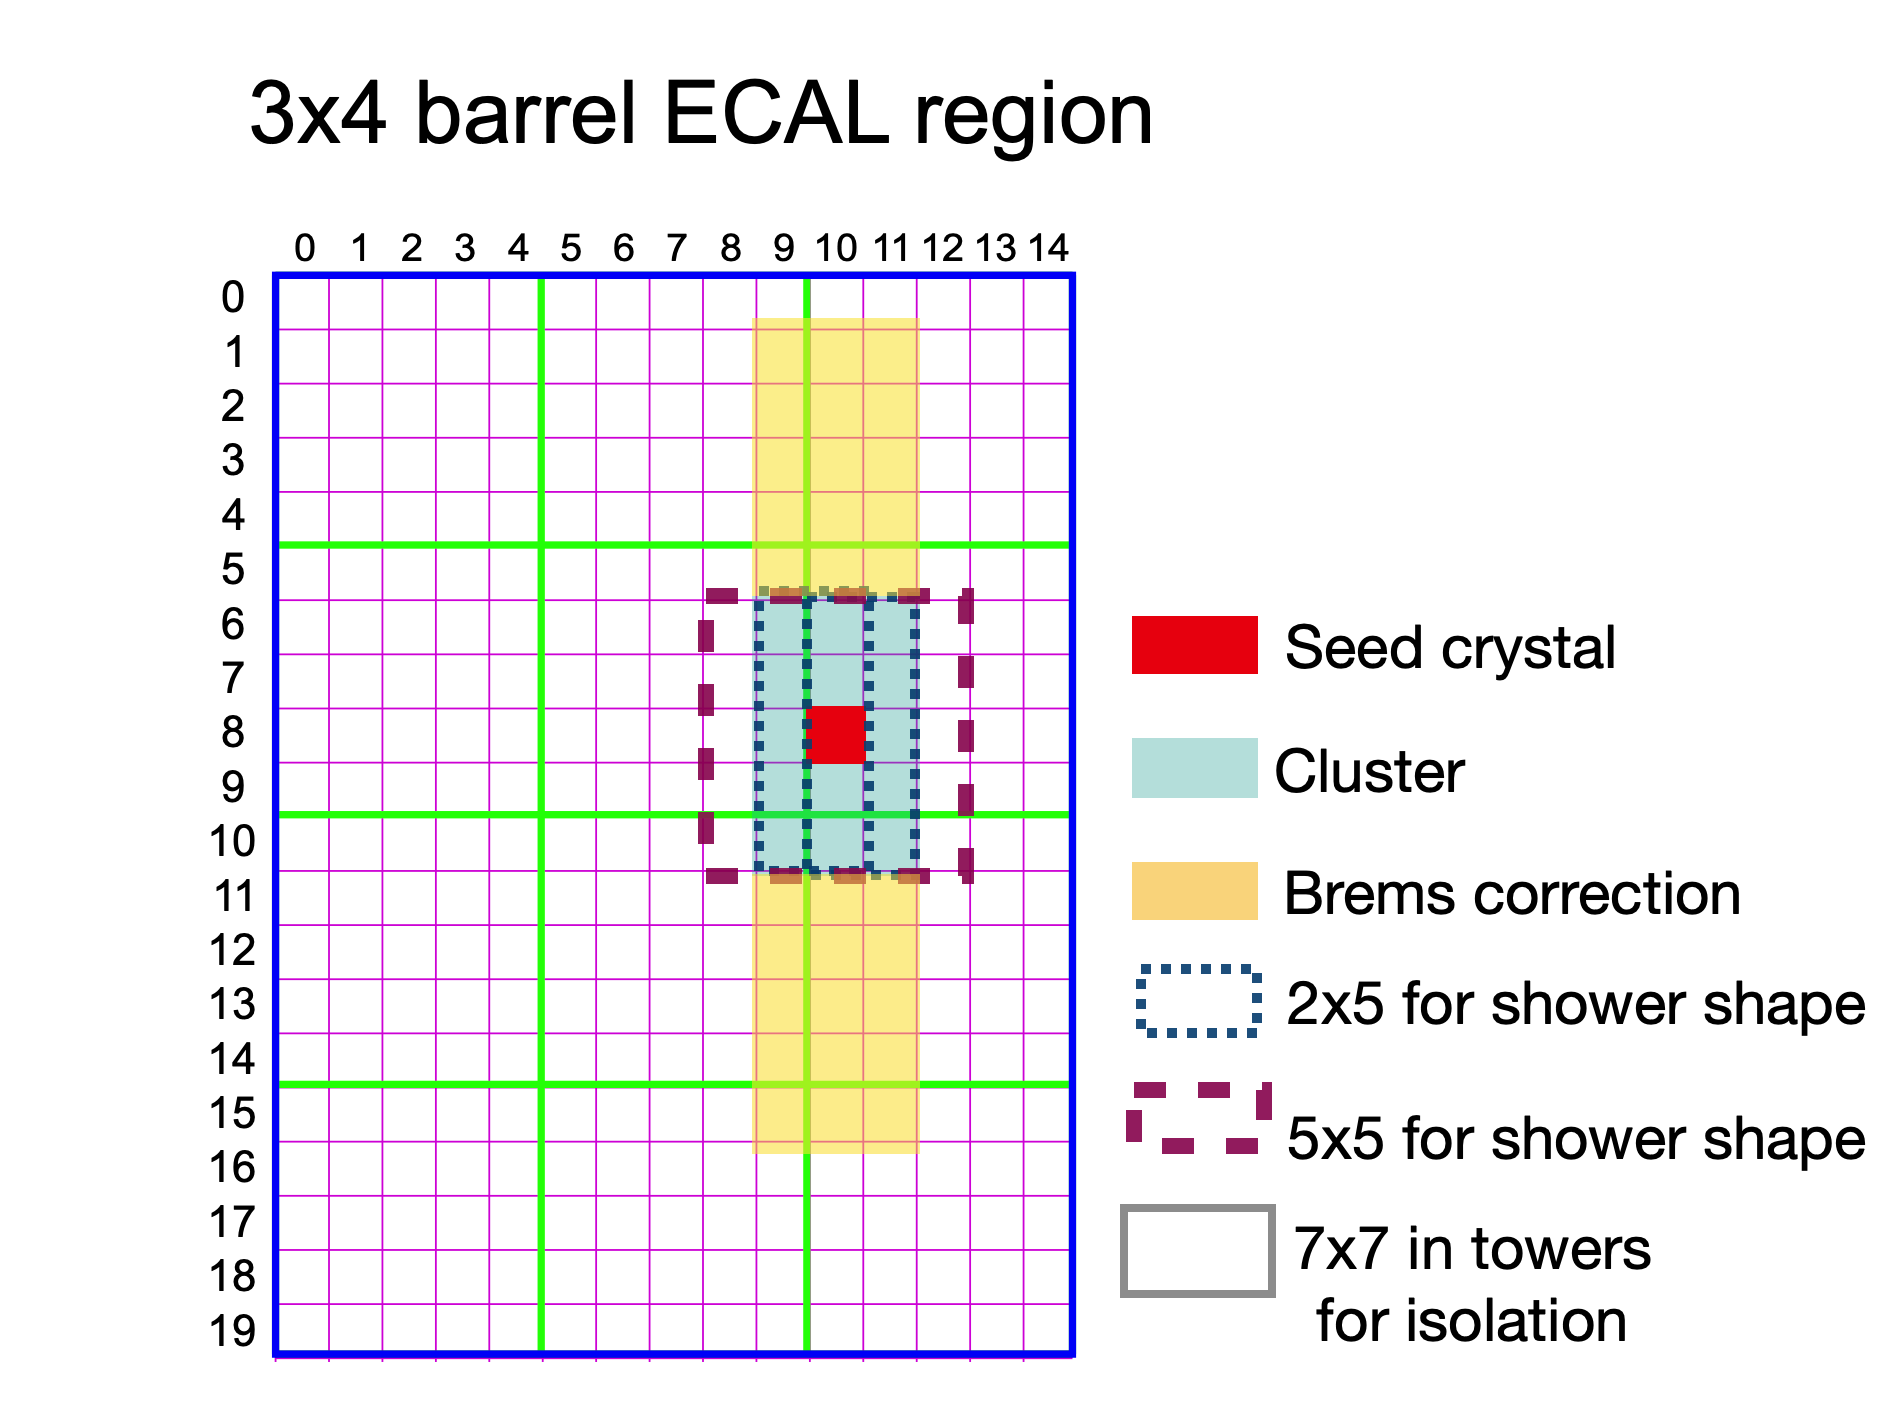
\includegraphics[width=12cm]{figures/ch-4-phase2/phase-2-cluster-footprint.png}
    \caption{Illustration of an example electron/photon ($e/\gamma$) cluster in the Phase-2 Level-1 Trigger standalone barrel $e/\gamma$ reconstruction, in a region of $15\times 20$ crystals ($3\times 4$ towers). Each small pink square is one crystal, the highest-granularity ECAL trigger primitives available to the L1 Trigger in Phase-2. The core cluster consists of the energy sum in a $3\times 5$ window of crystals, (\textit{shaded light blue}) centered around the seed crystal (\textit{red}). Bremsstrahlung corrections are checked in the adjacent $3\times 5$ windows in the $\phi$ direction (\textit{shaded light yellow}). The relative energies in windows of size $2\times 5$ and $5\times 5$ in crystals (\textit{dashed dark blue and dark red}) are used to compute shower shape variables to identify true $e/\gamma$ objects. Lastly, an isolation sum is computed in a window of size $7\times 7$ in towers (not shown in figure).}
    \label{fig:phase-2-cluster-footprint}
\end{figure}


In the RCT, an initial requirement of $p_{T} > 0.5$ GeV is imposed on the input trigger primitives (i.e. energies from the ECAL crystals and HCAL towers) to reject contribution from pileup. In one of the regions inside a RCT card (Fig. \ref{fig:phase-2-one-rct-card-schematic}), the crystal containing the highest energy deposit is identified as the seed crystal, as shown in Fig. \ref{fig:phase-2-cluster-footprint}. The energy in the crystals in a window of size $3\times 5$ in $\eta\times\phi$ around the seed cluster is added into a cluster. The energy is considered ``clustered''. The process is repeated with the remaining ``unclustered" energy, until up to four clusters are produced in the region. 


To improve $e/\gamma$ identification and to reduce background contributions, identification and reconstruction algorithms are implemented at this stage:
\begin{itemize}
    \item Shower shape: The energy deposit sums around the seed crystal is computed in windows of size $2 \times 5$ and $5 \times 5$ (Fig. \ref{fig:phase-2-cluster-footprint}, \textit{dashed lines}), with true $e/\gamma$ clusters tending to produce showers that deposit most of their energy in a $2 \times 5$ region. 
    \item Bremsstrahlung recovery: $e/\gamma$ tend to spread in the $\phi$ direction due to charged particles being bent by the magnetic field of the CMS solenoid. If sufficient energy comparable to the core $3 \times 5$ cluster is found in the adjacent $3 \times 5$ windows (Fig. \ref{fig:phase-2-cluster-footprint}, \textit{shaded yellow}), the energy is added to the core cluster and no longer considered unclustered energy.
\end{itemize}

After parallel processing in the regions, the clusters in a RCT card are stitched together if they are located directly along the borders of a region (Fig. \ref{fig:phase-2-rct-cards-schematic}). The remaining unclustered ECAL energy is summed into ECAL towers. 

From each RCT card, the twelve highest-energy clusters, as well as any remaining unclustered energy, are sent to the GCT. Since each GCT card has information from sixteen RCT cards (Fig. \ref{fig:phase-2-gct-cards-schematic}), final stitching across the boundaries of the RCT cards is performed. One more identification algorithm is performed at this stage:
\begin{itemize}
    \item Isolation: One handle to reject backgrounds from e.g. pileup, comes from the tendency for background to be spread more uniformly across a large area in the detector, whereas genuine $e/\gamma$ are expected to produce showers concentrated in the $3 \times 5$ crystal window. The energy sum in a large window of $7 \times 7$ in towers is computed and used to reject background.
\end{itemize}

\begin{figure}[ht]
    \centering
    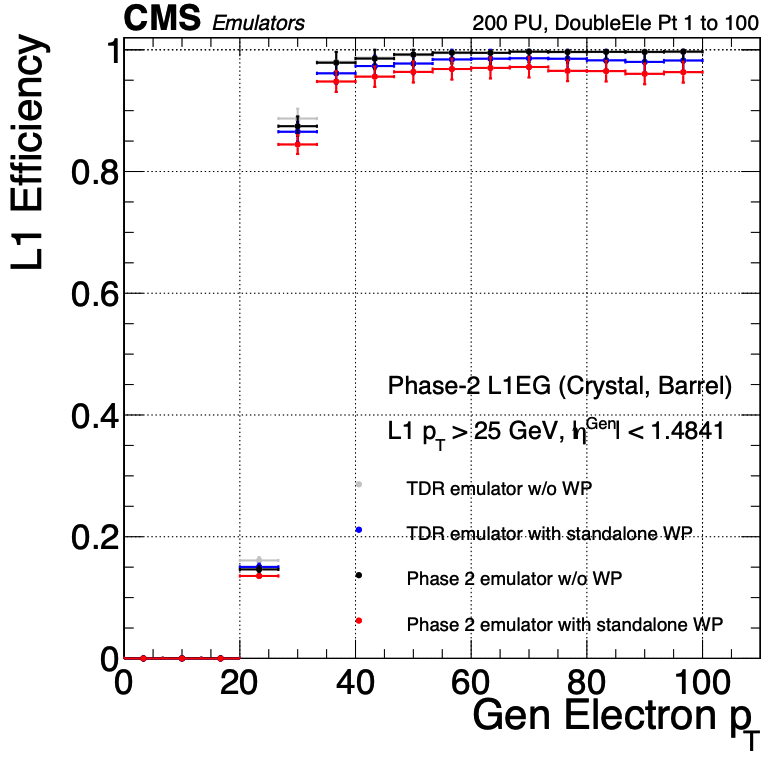
\includegraphics[width=12cm]{figures/ch-4-phase2/results-egamma-efficiency-gt25.png}
    \caption[Efficiency of the standalone barrel $e/\gamma$ reconstruction, as a function of the true electron's transverse momentum $p_{T}$.]{Efficiency of the standalone barrel $e/\gamma$ reconstruction, measured in a simulated sample of electrons, as a function of the true electron's transverse momentum $p_{T}$. The performance of the previous, idealized algorithm as shown in the 2021 Phase-2 TDR \cite{CMS-TDR-021} with and without the isolation and shower shape discrimination variables (``standalone working point/ WP'') (\textit{dark blue, grey}). The Phase-2 emulator discussed in this work with and without the same working point (\textit{black, red}) is shown to have comparable performance.}
    \label{fig:results-egamma-efficiency-gt25}
\end{figure}

\begin{figure}[ht]
    \centering
    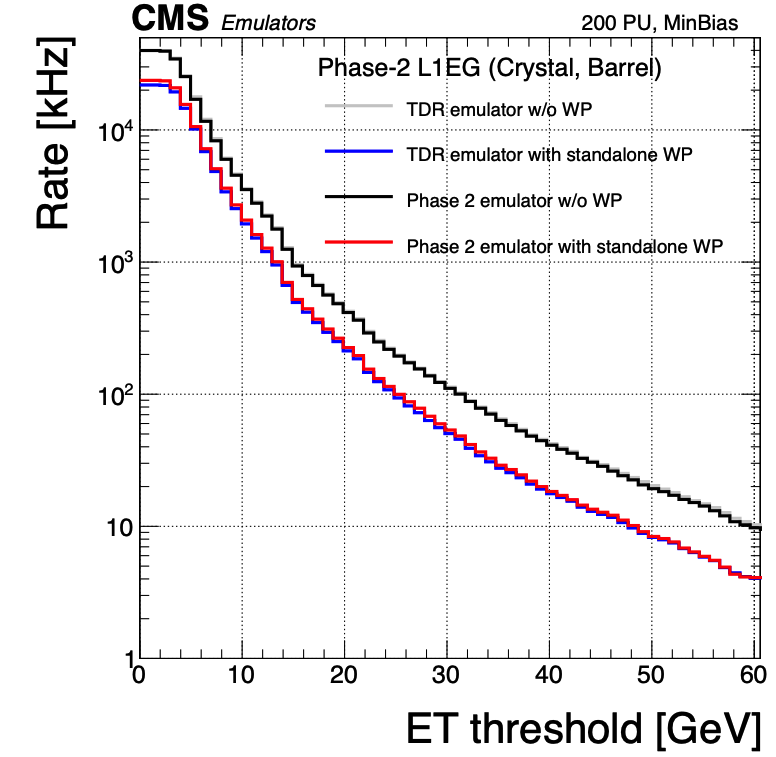
\includegraphics[width=12cm]{figures/ch-4-phase2/results-egamma-rates.png}
    \caption[Rates of the standalone barrel $e/\gamma$ reconstruction measured as a function of the minimum energy ($E_T$) required of the reconstructed $e/\gamma$ object in each event.]{Rates of the standalone barrel $e/\gamma$ reconstruction, evaluated on a minimum bias sample, measured as a function of the minimum energy ($E_T$) required of the reconstructed $e/\gamma$ object in each event. The performance of the previous, idealized algorithm as shown in the 2021 Phase-2 TDR \cite{CMS-TDR-021} with and without the isolation and shower shape discrimination variables (``standalone working point/ WP'') (\textit{dark blue, grey}). The Phase-2 emulator discussed in this work with and without the same working point (\textit{black, red}) is shown to have comparable performance.}
    \label{fig:results-egamma-rates}
\end{figure}


The performance of the standalone barrel $e/\gamma$ algorithm in Phase-2 conditions is summarized in the efficiency and rates. The efficiencies are measured with a simulated Monte Carlo sample containing electrons. The rates are measured with a simulated minimum bias sample intended to closely mimic generic proton-proton collisions in the CMS detector. The performance of the Phase-2 emulator discussed in this work, which closely mimics the firmware logic and uses fixed-precision integers, is shown to be comparable to the previous emulator which used floats and idealized logic.



\chapter{Event reconstruction}
We review the properties of the particles most pertinent to the analyes presented in this work (taus, muons, electrons, and b-jets), their resulting signatures in the CMS detector, and dedicated reconstruction techniques used at CMS.

\section{Taus}
Tau leptons, with a mass of 1.776 GeV, are heavy enough to decay hadronically (i.e. to final states with hadrons) which it does so about 64.8\% of the time. These hadronic decays are denoted $\tau_{h}$. The remainder of the time, it decays to final states with the lighter leptons (electron or muon), termed leptonic decays. In all cases, at least one is produced, resulting in missing transverse energy in the CMS detector. The tau's largest decay branching ratios (proportional to probability of decay) are listed below \citep{workman_review_2022}: 
\begin{itemize}
    \item 25.5\% decay to $\pi^- \pi^0 \nu_{\tau}$
    \item 17.8\% decay to $e^- \bar{\nu}_e \nu_{\tau}$
    \item 17.4\% decay to $\mu^- \bar{\nu}_\mu \nu_{\tau}$
    \item 10.8\% decay to $\pi^- \nu_{\tau}$ (excluding $K^0, \omega$)
    \item 9.3\% decay to $\pi^- 2\pi^0 \nu_{\tau}$ (excluding $K^0, \omega$)
    \item 9.0\% decay to $\pi^- \pi^- \pi^+ \nu_{\tau}$ (excluding $K^0, \omega$)
\end{itemize}

Thus in analyses containing $\tau\tau$ states, a distinction of the final states must be made for the possible combinatorics of the tau final states. For instance, a $\mu\tau_{h}$ event channel must be treated differently than a $\tau_{h}\tau_{h}$ channel.

In the CMS detector, charged pions leave tracks in the tracking detector before being absorbed in the hadronic calorimeter. Due to presence of the tracks for the charged pions, they are called ``prongs'' in hadronic tau reconstruction, giving gives rise to the names ``1 prong", ``1 prong + $\pi^0$(s)", and ``3-prong'' for the dominant hadronic tau decay modes. Neutral pions decay to two photons which lose their energy in the electromagnetic calorimeter. Taus that decay to electrons and muons, are typically triggered on and reconstructed as electrons and muons respectively. 

At CMS, hadronically decaying tau leptons are reconstructed with the hadron-plus-strips (HPS) algorithm \citep{CMS-TAU-14-001}, which is seeded with anti-$k_T$ jets. The HPS algorithm reconstructs $\tau_{h}$ candidates on the basis of the number of tracks and the number of ECAL strips in the $\eta-\phi$ plane with energy deposits, in the 1 prong, 1 prong + $\pi^0$(s), and 3-prong decay modes. A multivariate (MVA) discriminator, including isolation and lifetime information, is used to reduce backgrounds from quark- and gluon-initiated jets that are misidentified as $\tau_{h}$ candidates. 

\section{Muons}
Muons are identified with requirements on the quality of the track reconstruction and on the number of measurements in the tracker and the muon systems \citep{CMS-MUO-10-004}. In the standard CMS reconstruction, tracks are first reconstructed independently in the inner tracker (tracker track) and in the muon system (standalone-muon track). Next, these tracks are processed in two different methods. The first is Global Muon reconstruction (outside-in), which fits combined hits from the tracker track and standalone-muon track, using the Kalman-filter technique. At large transverse momenta, $p_{T} \gtrsim 200$ GeV, the global-muon fit can improve the momentum resolution compared to the tracker-only fit.  The second is Tracker Muon reconstruction (inside-out), which starts with tracker tracks with $p_{T} > 0.5$ GeV and total momentum $p_{T} > 2.5$ GeV. These tracks are extrapolated outwards to the muon system and matched to detector segments there, taking into account the magnetic field, expected energy losses, and multiple Coulomb scattering in the detector material. Tracker Muon reconstruction is more efficient than the Global Muon reconstruction at low momenta, $p \lesssim 5$ GeV, because it only requires a single muon segment in the muon system, where as Global Muon reconstruction typically requires segments in at least two muon stations.

\section{Electrons}
Electrons are identified with a multivariate discriminant combining several quantities describing the track quality, the shape of the energy deposits in the ECAL, and the compability of the the measurements from the tracker and the ECAL \citep{JINST-2015-10-P06005}.


\section{B-jets}





\chapter{Datasets and Monte Carlo samples}
\section{Datasets used}
The $h \rightarrow aa \rightarrow 2b2\tau$ analysis (CMS CADI line HIG-22-007) is based on proton-proton collision data at a center-of-mass energy of 13 TeV collected in full Run-2 (2016-18) with the CMS detector. The data analyzed corresponds to a total integrated luminosity of 138 fb$^{-1}$ (36.33 fb$^{-1}$ for 2016, 41.53 fb$^{-1}$ for 2017, and 59.74 fb$^{-1}$ for 2018) \cite{CMS-LUM-17-001} \cite{CMS-LUM-17-004} \cite{CMS-LUM-18-002}. 

Data collected with the single muon trigger is used for the $\mu\tau_{h}$ channel. For the $e\tau_{h}$ channel, data collected with the single electron trigger is used; and for the $e\mu$ channel, data collected with the electron $+$ muon trigger is used. A more in-depth discussion of the triggers used follows in a later section.

% TODO: put in this reference

\section{Monte Carlo samples}
Modeling and computing observables originating from arbitrary physics processes at the tree level and at next-to-leading order (NLO) is performed by Monte Carlo (MC) event generators, such as Powheg and MadGraph5\_amC\@NLO \cite{Alwall_2014} \cite{Frederix_2018}. The information generated, e.g. the computation of the differential cross sections and kinematics of the final state particles, is saved in a compressed file and used to generate MC samples that are used in physics analyses. The samples are digitized using GEANT4 \cite{agostinelli_geant4simulation_2003}, a platform used at the LHC and other facilities to comprehensively simulate the passage of particles through matter. The digitized samples are passed through the same detector reconstruction as real data events collected in the detector.

The samples for modeling the signal ($h \rightarrow aa \rightarrow 2b2\tau$ and $h\rightarrow a_1 a_2$) in the 2HDM+S and TRSM are generated at tree-level, for a range of masses of the light neutral scalar $a$. For $h \rightarrow aa$, the mass hypotheses for the $a$ range from $m_a = (12 \,\text{GeV}, 62.5 \,\text{GeV})$. For $h \rightarrow a_1 a_2$, the mass hypotheses for the two light scalars span combinations of $m_{a1}$, $m_{a2}$ ranging from $(12 \,\text{GeV}, 62.5 \,\text{GeV})$ for the two scalars.

% TODO: put table of samples

\section{Embedded samples}
An embedding technique is used to estimate background from the Standard Model $Z$ boson decaying to $\tau\tau$, from data with minimal simulation input \cite{CMS-TAU-18-001}. In data events selected to have $Z \rightarrow \mu\mu$ decays, all energy deposits of the recorded muons are removed from the event, and replaced with simulated tau leptons with the same kinematic properties as the removed muons. This results in a hybrid data format containing information from both observed and simulated events. The advantage of the Embedded samples is that the portions of the event that are difficult to model and describe (e.g. the underlying event or production of additional jets) are directly taken from data. 

% TODO: put table of Embedded samples

\chapter{Event selection}
For the search for $h \rightarrow aa \rightarrow 2b2\tau$, three final states of the $\tau\tau$ system are considered: $\mu\tau_{h}$, $e\tau_{h}$, and $e\mu$. The $\tau_{h}\tau_{h}$ final state is not considered because signal events in the $\tau_{h}\tau_{h}$ channel would typically produce hadronic taus with momenta below data-taking trigger thresholds.

In all three final states, events are required to pass at least one b-tag jet passing the medium working point of the DeepFlavour tagger, with $p_{T} > 20$ GeV, and $|\eta| < 2.4$. A second b-tag jet is not required because such a requirement would reduce signal acceptance by 80\% compared to only requiring one b-tag jet.

Events in data, MC samples, and Embedded samples are sorted into one of the three $\tau\tau$ channels if they pass the following trigger requirements and requirements on the offline reconstructed objects in the event. The two leading leptons (e.g. muon and hadronic tau for the $\mu\tau_{h}$ channel) determined to have originated from the $\tau\tau$ decay, are called the leading ``legs'' and are respectively subscripted $1$ and $2$ in this work.


\section{$\mu\tau_{h}$ channel}

A single muon trigger is used if the muon has sufficiently high $p_{T}$, otherwise a dilepton $\mu\tau_{h}$ cross-trigger is used. For data taken in 2017-2018 (2016), the logical OR of the single muon triggers with online $p_{T}$ thresholds 24 and 27 (23) GeV is used, with the corresponding offline muon required to have with $p_{T}$ 1 GeV above the online threshold. For data taken in 2017-2018 (2016), a dilepton $\mu + \tau_{h}$ cross-trigger with $p_{T}$ thresholds of 20 (19) and 27 (20) GeV for the muon and tau respectively, is used. The $\tau_{h}$ is required to have $|\eta| < 2.3$ if the single trigger is fired, $|\eta| < 2.1$. 

\section{$e\tau_{h}$ channel}

Similarly to the $\mu\tau_{h}$ channel, a single electron trigger is used if the electron has sufficiently high $p_{T}$ in 2018 and 2017. For data taken in 2018 (2017), the OR of the single electron triggers with online $p_{T}$ thresholds at 32 and 35 (27 and 32) GeV are used, with the corresponding offline electrons required to have $p_{T}$ greater than 33 (28) GeV. A $e + \tau_{h}$ cross-trigger is used for electrons with lower offline $p_{T}$ between 25 and 33 GeV (25 and 28 GeV). For the 2016 dataset, there is no cross trigger but only a single electron trigger with online $p_{T}$ threshold at 25 GeV, which is used if the offline electron has $p_{T}$ greater than 26 GeV.

\section{$e\mu$ channel}

In the $e\mu$ channel, events are selected with the logical OR of two $e+\mu$ cross triggers: electron with online $p_{T} > 23$ GeV and muon with online $p_{T} > 8$ GeV, or electron with online $p_{T} > 12$ GeV and muon with online $p_{T}>23$ GeV. The corresponding offline objects are required to have offline $p_{T}$ several GeV greater than than the online thresholds.

\chapter{Scale factors and corrections}
\label{chapter:ch-8:scale-factors-and-corrections}
As the modeling of the CMS detector and underlying physics processes are imperfect, scale factors and corrections are applied to Monte Carlo events and in some cases, the embedded samples, to improve agreement with measurements in data. For the standard reconstruction physics objects in this work, central recommendations provided by dedicated physics object groups (POGs) in CMS are used.

Uncertainties in scale factors and corrections are also sources of systematic errors in the analysis, detailed in Chapter \ref{chapter:ch-12:systematic-uncertainties}. Systematic uncertainties in the tau, muon, and electron energy scales can shift the $p_{T}$ of the leptons up or down, causing a migration of number of events that pass the offline $p_{T}$ thresholds described in the previous section.

\section{Tau energy scale}
\label{sec:tau_energy_scale}

An energy scale is applied to the transverse momentum $p_{T}$ and mass of the hadronic tau $\tau_{h}$ in the $\mu\tau_{h}$ and $e\tau_{h}$ channels, to correct for a deviation of the average reconstructed $\tau_{h}$ energy from the generator-level energy of the visible $\tau_{h}$ decay products. These correction factors are derived centrally \cite{CMS-TAU-16-003}, by fitting to events in $e\tau_{h}$ and $\mu\tau_{h}$ final states in $Z/\gamma^*$ events separately for the $h^\pm$, $h^\pm \pi^0$, and $h^\pm h^\mp h^\pm$ decays. The values used are shown in Table \ref{table:tau-ES}.

When applying the energy scale to the $\tau_{h}$, the 4-momentum of the missing transverse energy (MET) is adjusted such that the total 4-momenta of the $\tau_{h}$ and the MET remains unchanged \cite{twiki_TAU_POG_tauidrecommendationforrun2}.

\begin{table}[ht]
    \centering
    \begin{tabular}{|c|c|c|c|c|}
    \hline
    \multicolumn{5}{|c|}{Tau energy scale factor}                                   \\ \hline
    \hline
    Decay mode      & 2018              & 2017              & 2016 pre-VFP      & 2016 post-VFP     \\ \hline
    0               & 0.991 $\pm$ 0.008 & 0.986 $\pm$ 0.009 & 0.987 $\pm$ 0.01  & 0.993 $\pm$ 0.009 \\
    1               & 1.004 $\pm$ 0.006 & 0.999 $\pm$ 0.006 & 0.998 $\pm$ 0.006 & 0.991 $\pm$ 0.007 \\
    10              & 0.998 $\pm$ 0.007 & 0.999 $\pm$ 0.007 & 0.984 $\pm$ 0.008 & 1.001 $\pm$ 0.007 \\
    11              & 1.004 $\pm$ 0.009 & 0.996 $\pm$ 0.01  & 0.999 $\pm$ 0.011 & 0.997 $\pm$ 0.016 \\ \hline
    \end{tabular}
    \caption{Energy scales applied to genuine hadronic tau decays $\tau_{h}$ by data-taking year/era and decay mode, along with systematic errors.}
    \label{table:tau-ES}
\end{table}

\section{Muon energy scale}
\label{sec:muon_energy_scale}

An energy scale is applied to the $p_{T}$ and mass of genuine muons from $\tau$ decays in the $e\mu$ and $\mu\tau_{h}$ channels \cite{twiki_MUON_POG_recommendation}. The applied values are the same for MC and embedded samples and are shown in Table \ref{table:muon-ES}. Following the SM $H \rightarrow \tau\tau$ analysis, Rochester corrections are not applied, and instead prescriptions from \cite{twiki_MUO_simplified_ES} are followed.


\begin{table}[ht]
    \centering
    \begin{tabular}{|c|c|}
    \hline
    \multicolumn{2}{|c|}{Muon energy scale factor}      \\ \hline
    \hline
    Eta range                & Value for all years \\ \hline
    $|\eta| \in [0.0, 1.2)$  & 1.0 $\pm$ 0.004 \\
    $|\eta| \in [1.2, 2.1)$  & 1.0 $\pm$ 0.009 \\
    $|\eta| \in [2.1, 2.4)$  & 1.0 $\pm$ 0.027 \\
    \hline
    \end{tabular}
    \caption[Energy scales and systematic errors applied to genuine muons.]{Energy scales and systematic errors applied to genuine muons. The values are the same for MC and embedded for all years \cite{twiki_HiggsToTauTauWorkingLegacyRun2} \cite{twiki_MUO_simplified_ES}.}
    \label{table:muon-ES}
\end{table}


\section{Electron energy scale}
\label{sec:electron_energy_scale}

Corrections to the electron energy scale are applied to genuine $e$ from $\tau$ decays, and are binned in two dimensions by electron $p_{T}$ and $\eta$ for barrel vs. endcap \cite{twiki_Electron_POG_recommendation}. The scale factors are binned in $p_{T}$ and $\eta$ for MC samples: e.g. values for 2018 are shown in Fig. \ref{fig:egamma-POG-UL-egamma-scale-factors} from \cite{twiki_Electron_UL_2016_2017_2018}. For embedded samples the electron energy scale is taken as only binned in $\eta$ (Table \ref{table:ele-ES-embedded}).

% https://twiki.cern.ch/twiki/pub/CMS/EgammaUL2016To2018/egammaEffi.txt_Ele_wp90noiso_egammaPlots.pdf
\begin{figure}[h]
    \centering
    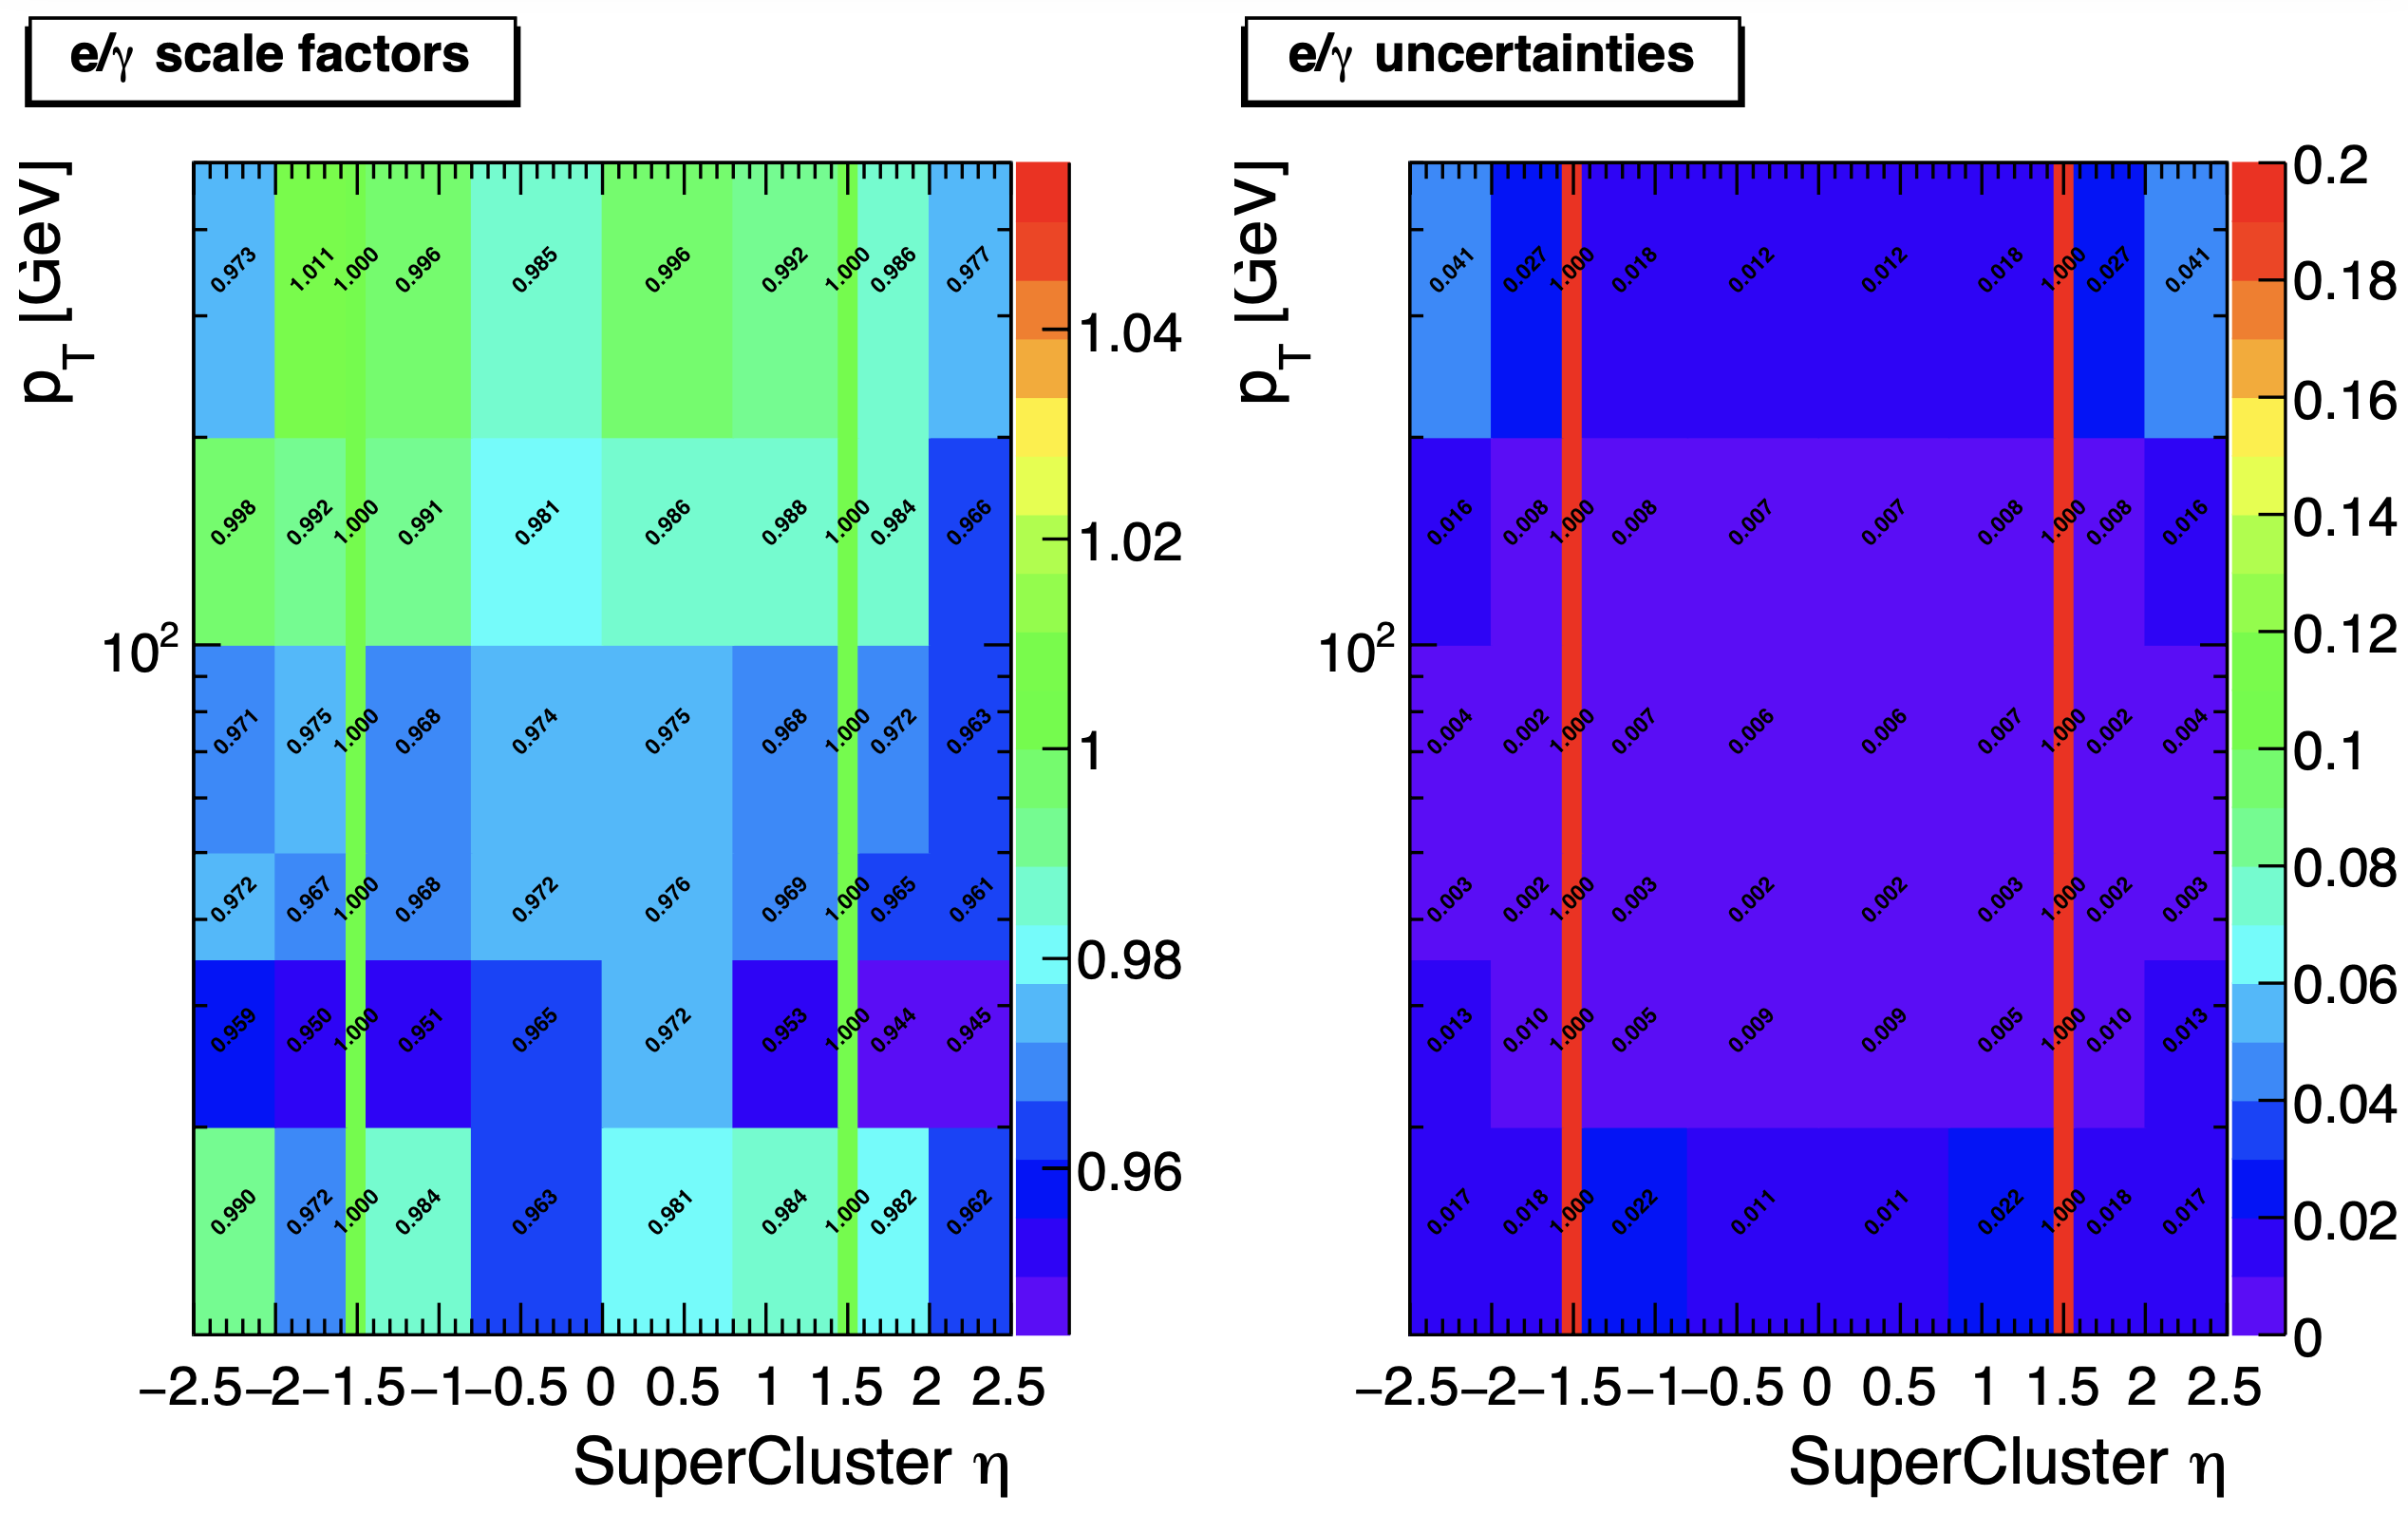
\includegraphics[width=15cm]{figures/ch-8-scale-factors-and-corrections/egamma-POG-UL-egamma-scale-factors.png}
    \caption[Electron/photon energy scale factors and uncertainties for 2018.]{Electron/photon energy scale factors (\textit{left}) and corresponding uncertainties (\textit{right}) binned in the electron $\eta$ and $p_{T}$, for the data-taking year 2018 \cite{twiki_Electron_UL_2016_2017_2018}.} 
    \label{fig:egamma-POG-UL-egamma-scale-factors}
\end{figure}


\begin{table}[h]
    \centering
    \begin{tabular}{|c|c|c|c|}
    \hline
    \multicolumn{4}{|c|}{Electron energy scale factor for embedded samples}                                   \\ \hline
    \hline
    Eta range                   & 2018               & 2017               & 2016     \\ \hline
    $|\eta| \in [0.0, 1.479)$   & 0.973 $\pm$ 0.005  & 0.986 $\pm$ 0.009  & 0.9976 $\pm$ 0.0050 \\
    $|\eta| \in [1.479, 2.4)$   & 0.980 $\pm$ 0.0125 & 0.887 $\pm$ 0.0125 & 0.993 $\pm$ 0.0125 \\ \hline
    \end{tabular}
    \caption[Energy scales and systematic errors applied to electrons in embedded samples by data-taking year/era.]{Energy scales and systematic errors applied to electrons in embedded samples, binned in the electron $\eta$, by data-taking year \cite{twiki_embedded_preUL_2016} \cite{twiki_embedded_preUL_2017} \cite{twiki_embedded_preUL_2018}.}
    \label{table:ele-ES-embedded}
\end{table}

\section{$\tau_{h}$ identification efficiency}
\label{sec:tauh_id_efficiency}

The $\tau_{h}$ identification efficiency can differ in data and MC \cite{twiki_TAU_POG_tauidrecommendationforrun2}. Recommended corrections are provided by the Tau POG, and we use the medium DeepTau vs. jet working point values. The identification efficiency is measured in $Z \rightarrow \tau\tau$ events in the $\mu\tau_{h}$ final state, and is binned in $p_{T}$ due to clear $p_{T}$ dependence of the DeepTau ID. 


\begin{table}[h]
    \centering
    \begin{tabular}{|c|c|c|c|c|c|c|}
    \hline
    \multicolumn{7}{|c|}{Tau ID efficiency for DeepTau Medium vs. jet WP in 2018}                                   \\ \hline
    \hline
    $p_{T}$ (GeV)  & $<20$  & $(20, 25]$ & $(25, 30]$ & $(30, 35]$ & $(35, 40]$ & $(40, 500] $   \\ \hline
    Central value  & 0      & 0.945      & 0.946      & 0.916      & 0.921      & 1.005 \\
    Up value       & 0      & 1.001      & 0.981      & 0.946      & 0.950      & 1.035 \\
    Down value     & 0      & 0.888      & 0.981      & 0.883      & 0.893      & 0.953 \\ \hline
    \end{tabular}
    \caption[Tau ID efficiency for the DeepTau vs. jet medium working point, with central, up, and down values for 2018, binned in the tau $p_{T}$.]{Tau ID efficiency for the DeepTau vs. jet medium working point, with central, up, and down values for 2018, binned in the tau $p_{T}$ \cite{twiki_TAU_POG_tauidrecommendationforrun2}.}
    \label{table:tauIDeff_deepTau_vs_jet_medium_WP}
\end{table}


\section{Trigger efficiencies}

Scale factors are applied to correct for differences in trigger efficiencies between MC and embedded vs. data, with values taken from tools provided by the Standard Model $H \rightarrow \tau\tau$ working group which uses the same trigger paths \cite{twiki_HiggsToTauTauWorkingLegacyRun2}. In the following sections we review relevant trigger efficiencies in data, which form the basis of the trigger efficiency corrections applied to MC and embedded.

\subsection{Tau trigger efficiencies}
The efficiencies in data of the single-$\tau_{h}$ leg in $\mu\tau_{h}$, $e\tau_{h}$, and di-$\tau_{h}$ triggers is computed centrally per using a Tag and Probe (TnP) method \cite{CMS-DP-2019-012} which is outlined here. In this method, $Z \rightarrow \tau\tau \rightarrow \mu\tau_{h}$ are selected in data and a Drell-Yan simulated sample ($Z \rightarrow \ell\ell, \ell = e, \mu, \tau_{h}$) with high purity. Cuts are applied to reject events not in this final state, e.g. suppressing $Z \rightarrow \mu\mu$ by vetoing events with a single loose ID muon. An isolated muon candidate (the tag) with online $p_{T} > 27$ GeV and $|\eta| < 2.1$ is identified and matched to an offline $\mu$. An offline $\tau_{h}$ candidate (the probe) is selected, which is separated from the tag $\mu$, and has $p_{T} > 20$ GeV and $|\eta| < 2.1$. The probe $\tau_{h}$ must pass anti-muon and anti-electron discriminators to avoid fakes from muons and electrons, and must pass the medium MVA tau isolation to suppress fakes from QCD jets. The trigger efficiency in the TnP method is calculated as 
\begin{equation}
    \text{Efficiency} = \frac{\text{Number of events passing the TnP selection with fires the HLT path}}{\text{Number of events passing the TnP selection}}
\end{equation}


The efficiencies for the hadronic tau legs in the relevant channels of this analyses ($\mu\tau_{h}$ and $e\tau_{h}$) as a function of the offline tau $p_{T}$ and $\eta$, are shown for data taken in 2016, 2017, and 2018 in Figures \ref{fig:mutauEfficiencyPt_eachYear_mediumTauMVA_Data} and \ref{fig:etauEfficiencyPt_eachYear_mediumTauMVA_Data} \cite{CMS-DP-2019-012} \cite{twiki_Tau_Lepton_Run_2_trigger_performance}. In both figures, the different HLT thresholds and differences in the L1 seed result in higher efficiencies in 2016 and differences in shapes of the 2016 efficiencies compared to 2017 and 2018. The low pileup in 2016 also leads to higher efficiencies in that year.


\begin{figure}[h]
    \centering
    \begin{subfigure}{0.45\textwidth}
        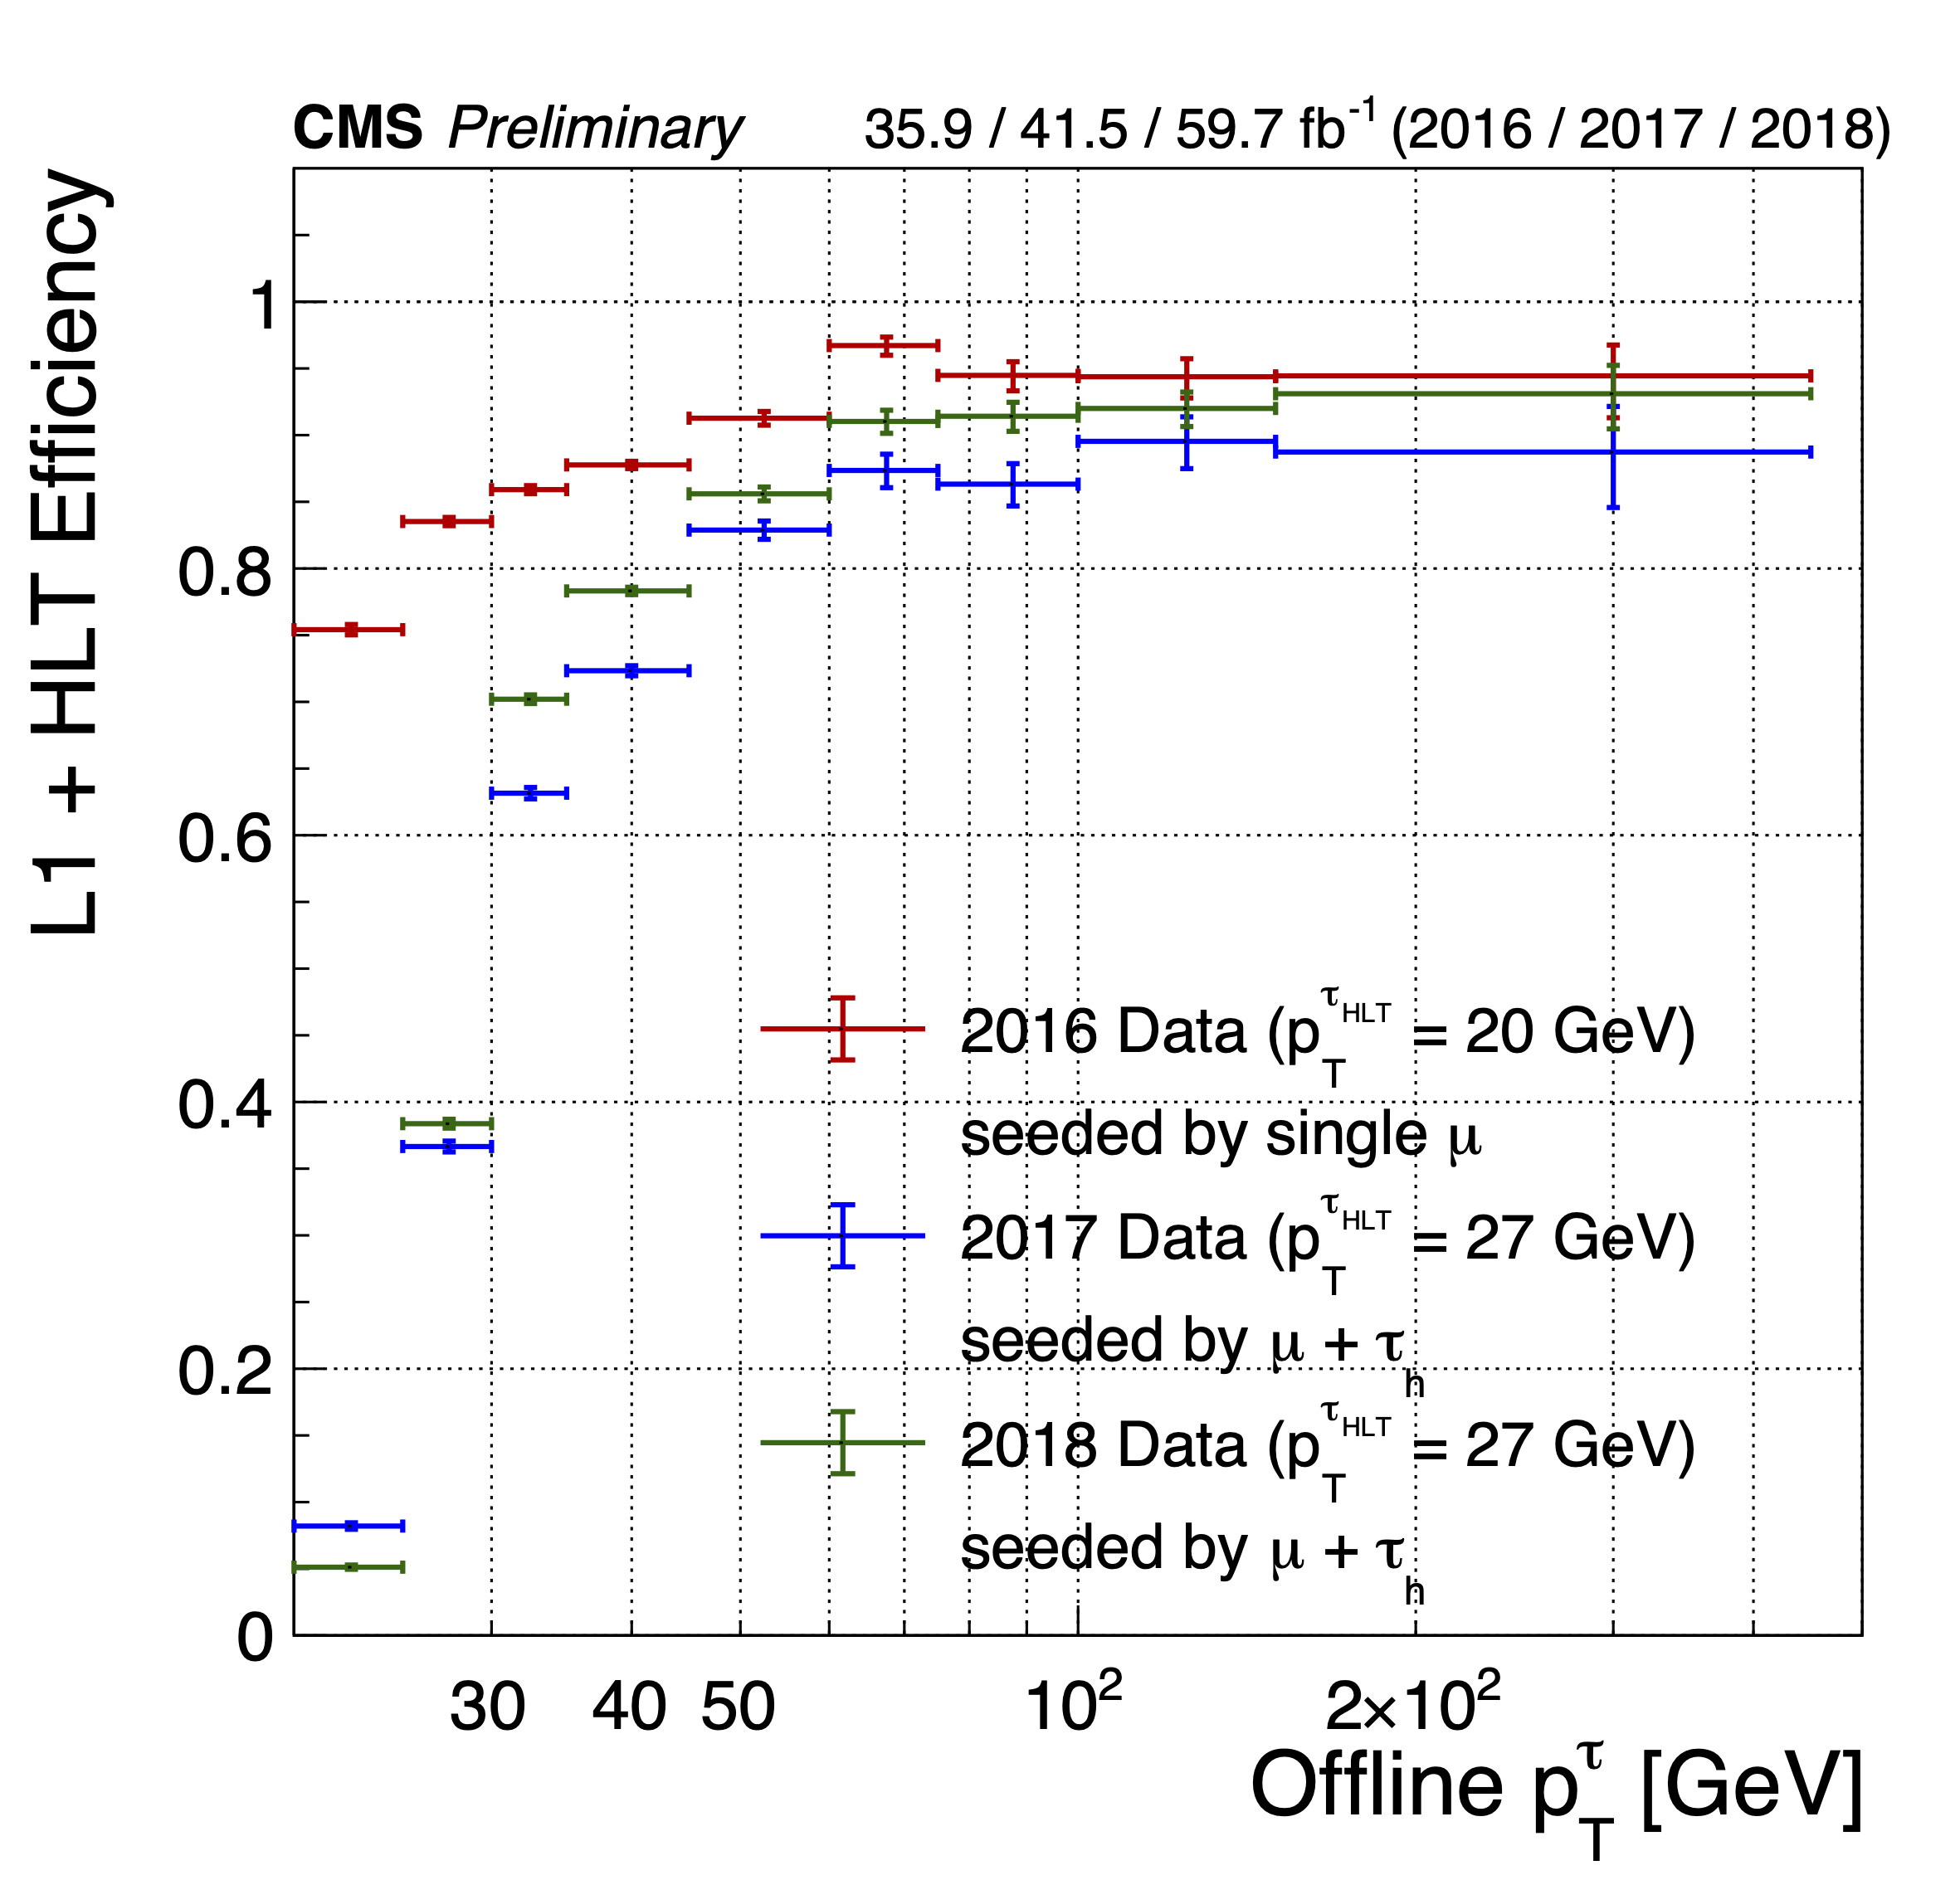
\includegraphics[width=1.0\textwidth]{figures/ch-8-scale-factors-and-corrections/mutauEfficiencyPt_eachYear_mediumTauMVA_Data.png}
        \caption{$\tau_{h}$ efficiency from $\mu\tau_{h}$ trigger.}
        \label{fig:mutauEfficiencyPt_eachYear_mediumTauMVA_Data}
    \end{subfigure}
    \hfill
    \begin{subfigure}{0.45\textwidth}
        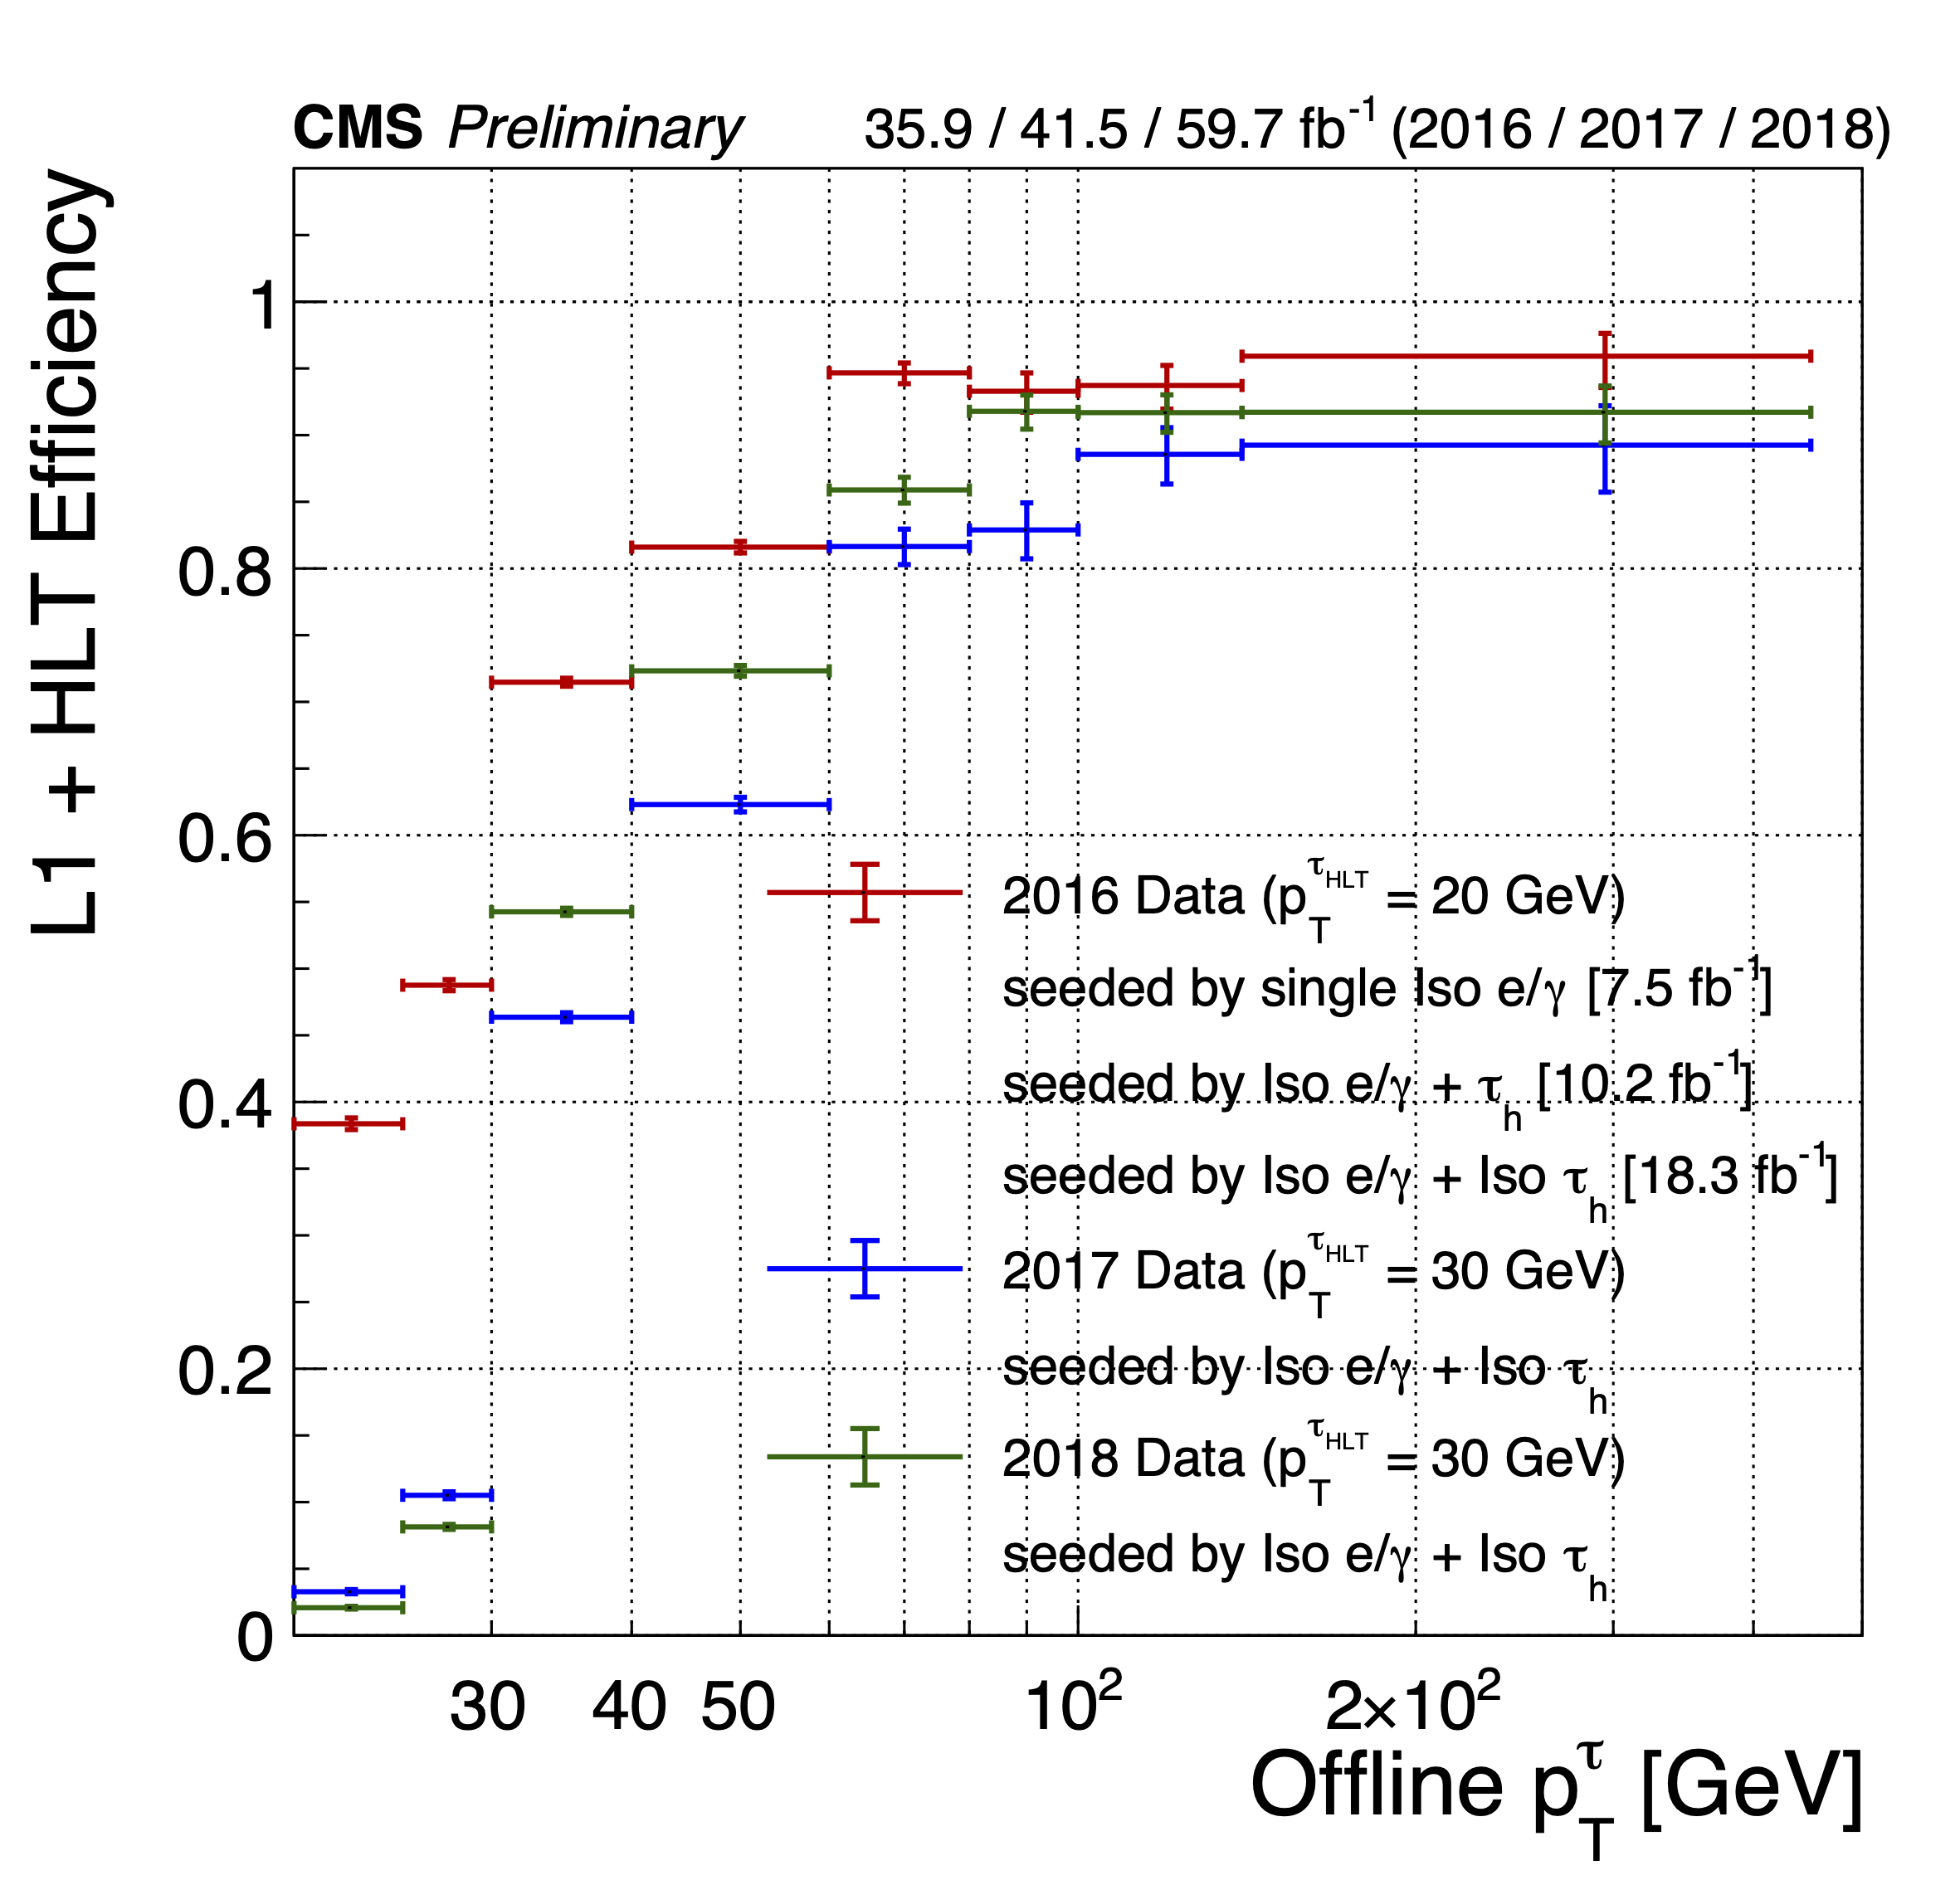
\includegraphics[width=1.0\textwidth]{figures/ch-8-scale-factors-and-corrections/etauEfficiencyPt_eachYear_mediumTauMVA_Data.png}
        \caption{$\tau_{h}$ efficiency from $e\tau_{h}$ trigger.}
        \label{fig:etauEfficiencyPt_eachYear_mediumTauMVA_Data}
    \end{subfigure}
    \caption[Hadronic tau leg efficiency of the cross-triggers for $\mu\tau_{h}$ (\textit{left}) and $e\tau_{h}$ (\textit{right}) triggers as a function of offline tau $p_{T}$ for 2016, 2017, and 2018.]{Hadronic tau leg efficiency of the cross-triggers for $\mu\tau_{h}$ (\textit{left}) and $e\tau_{h}$ (\textit{right}) triggers as a function of offline tau $p_{T}$ for the years 2016 (\textit{red}), 2017 (\textit{blue}) and 2018 (\textit{green}), from \cite{twiki_Tau_Lepton_Run_2_trigger_performance}. HLT $p_{T}$ thresholds and L1 seeds are indicated in the legends.} 
\end{figure}


\subsection{Single muon trigger efficiencies}
The efficiencies for the single isolated muon trigger with $p_{T} > 24$ GeV used in this analysis, is shown for the data-taking year 2018 in Fig. \ref{fig:single_muon_24GeV_efficiency_vs_pt} as a function of the muon $p_{T}$ and as a function of the muon $|\eta|$ in Fig. \ref{fig:single_muon_24GeV_efficiency_vs_eta} from \cite{CMS-DP-2018-034}. The data is split with respect to a HLT muon reconstruction update that was deployed on 15/05/2018. A small asymmetry in efficiencies between negative and positive $\eta$ in Fig. \ref{fig:single_muon_24GeV_efficiency_vs_eta} is due to disabled muon chambers (CSCs). The efficiencies shown are estimated using a Tag and Probe method using $Z\rightarrow \mu\mu$ events, with the tag being an offline muon with $p_{T} > 29$ GeV and $|\eta| < 2.4$ passing a tight ID criteria, and the probe is an online (L1) trigger object with $\Delta R < 0.3$ and passing tight ID and Particle Flow based isolation requirements with $p_{T} > 26$ GeV.

\begin{figure}[h]
    \centering
    \begin{subfigure}{0.45\textwidth}
        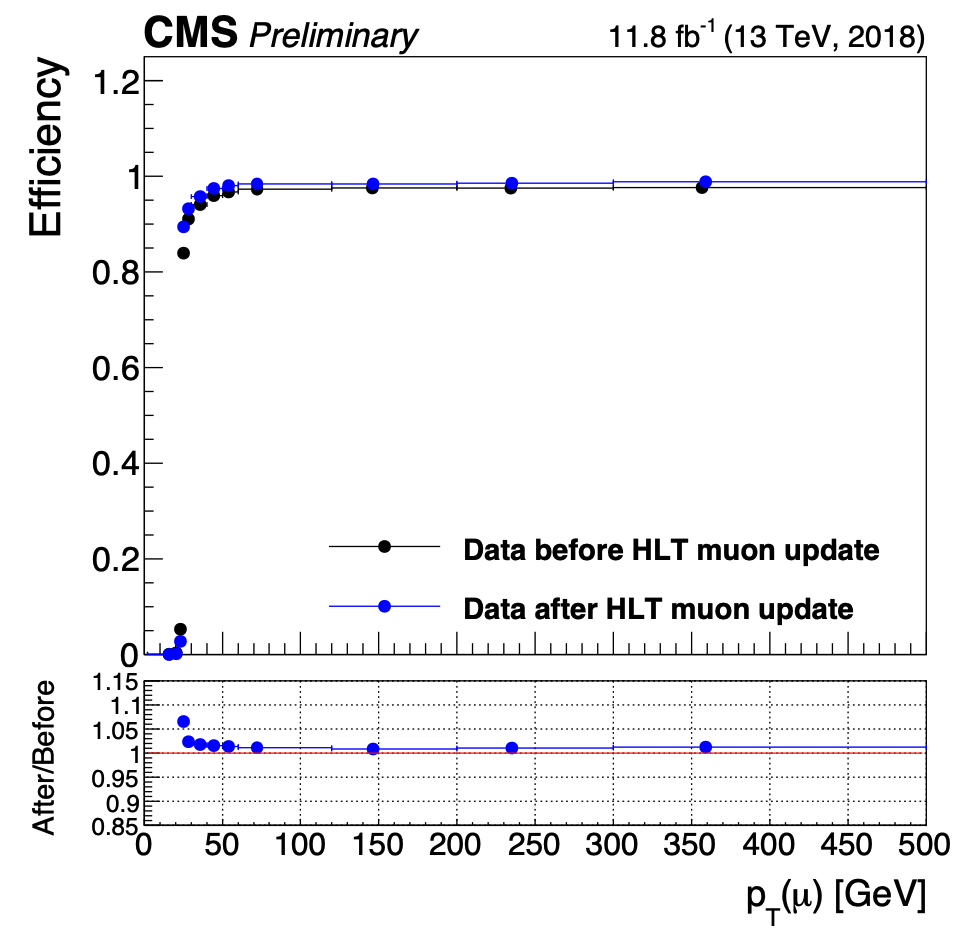
\includegraphics[width=1.0\textwidth]{figures/ch-8-scale-factors-and-corrections/singleMuon_isolated_efficiency_vs_pt}
        \caption{Muon efficiency vs $p_{T}$ for SingleMuon.}
        \label{fig:single_muon_24GeV_efficiency_vs_pt}
    \end{subfigure}
    \hfill
    \begin{subfigure}{0.45\textwidth}
        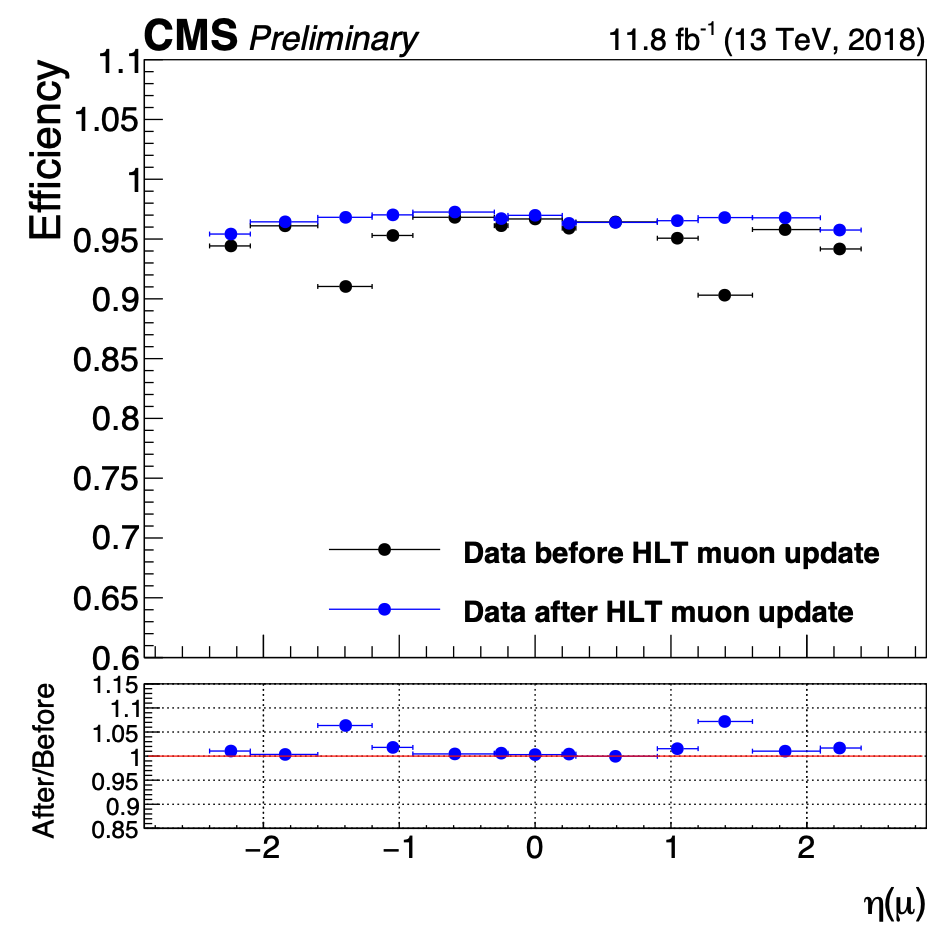
\includegraphics[width=1.0\textwidth]{figures/ch-8-scale-factors-and-corrections/singleMuon_isolated_efficiency_vs_eta}
        \caption{Muon efficiency vs $|\eta|$ for SingleMuon.}
        \label{fig:single_muon_24GeV_efficiency_vs_eta}
    \end{subfigure}
    \caption[Trigger efficiencies in data (\textit{top panels}) and ratio of efficiencies after/before a HLT muon reconstruction update (\textit{bottom panels}) for the muon in the isolated single muon trigger with threshold $p_{T} > 24$ GeV in the data-taking year 2018, as functions of the muon $p_{T}$ (\textit{left}) and muon $|\eta|$ (\textit{right}).]{Trigger efficiencies in data (\textit{top panels}) and ratio of efficiencies after/before a HLT muon reconstruction update (\textit{bottom panels}) for the muon in the isolated single muon trigger with threshold $p_{T} > 24$ GeV in the data-taking year 2018, as functions of the muon $p_{T}$ (\textit{left}) and muon $|\eta|$ (\textit{right}). Only statistical errors are shown \cite{CMS-DP-2018-034}.} 
\end{figure}

\subsection{Single electron trigger efficiencies}

The efficiencies in data, and the ratio between data and MC, of the single electron HLT trigger with $p_{T}$ threshold 32 GeV used in this analysis are shown for 2018, as a function of the electron $p_{T}$ in Fig. \ref{fig:single_ele_32GeV_efficiency_vs_pt} and of the electron $|\eta|$ in Fig. \ref{fig:single_ele_32GeV_efficiency_vs_eta}, from \cite{CMS-DP-2020-016}. In the Tag and Probe method used for the 2018 dataset, the tag is an offline reconstructed electron with $|\eta| \leq 2.1$ and not in the barrel and endcap overlap region, with $p_{T} > 35$ GeV with tight isolation and shower shape requirements, firing the tag trigger. The probe is an offline reconstructed electron with $|\eta| \leq 2.5$ with $E_T^\text{ECAL} > 5$ GeV with no extra identification criteria \cite{CMS-DP-2020-016}. 

The disagreement between data and MC, particularly at low transverse momentum, is in part due to detector effects that are difficult to simulate, such as crystal transparency losses in the ECAL and the evolution of dead regions in the pixel tracker \cite{CMS-DP-2020-016}.

\begin{figure}[h]
    \centering
    \begin{subfigure}{0.45\textwidth}
        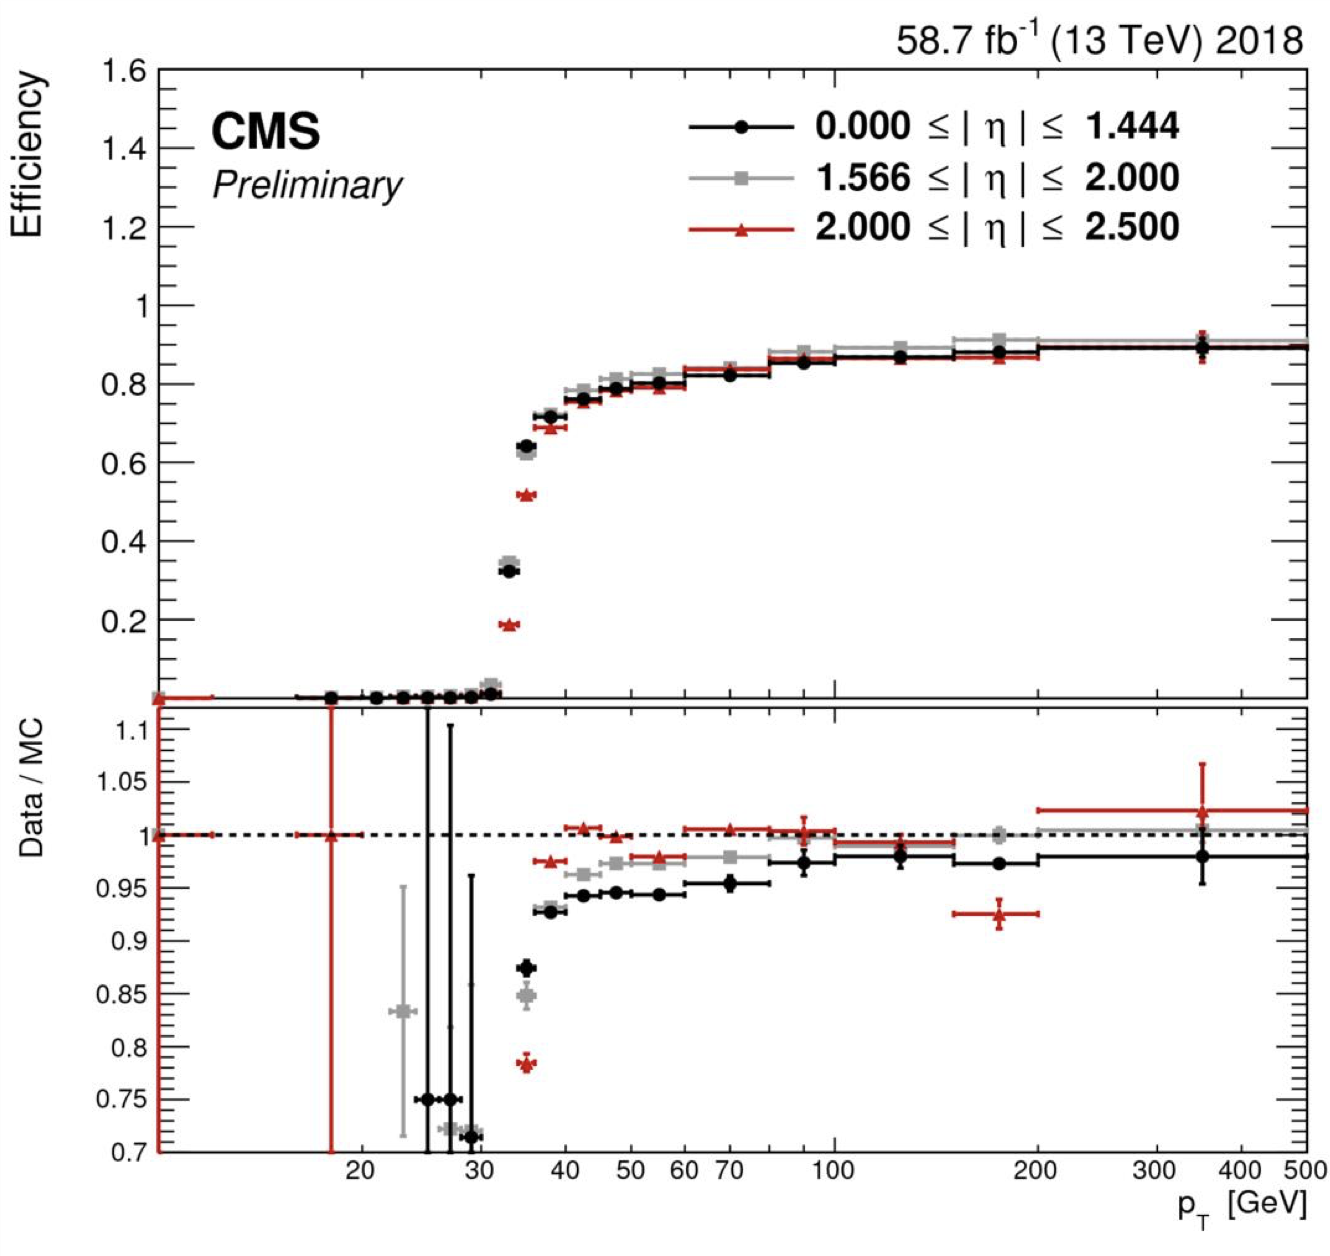
\includegraphics[width=1.0\textwidth]{figures/ch-8-scale-factors-and-corrections/electron_Ele32_WPTight_Gsf_efficiency_vsPt}
        \caption{Electron efficiency vs $p_{T}$ for single electron.}
        \label{fig:single_ele_32GeV_efficiency_vs_pt}
    \end{subfigure}
    \hfill
    \begin{subfigure}{0.45\textwidth}
        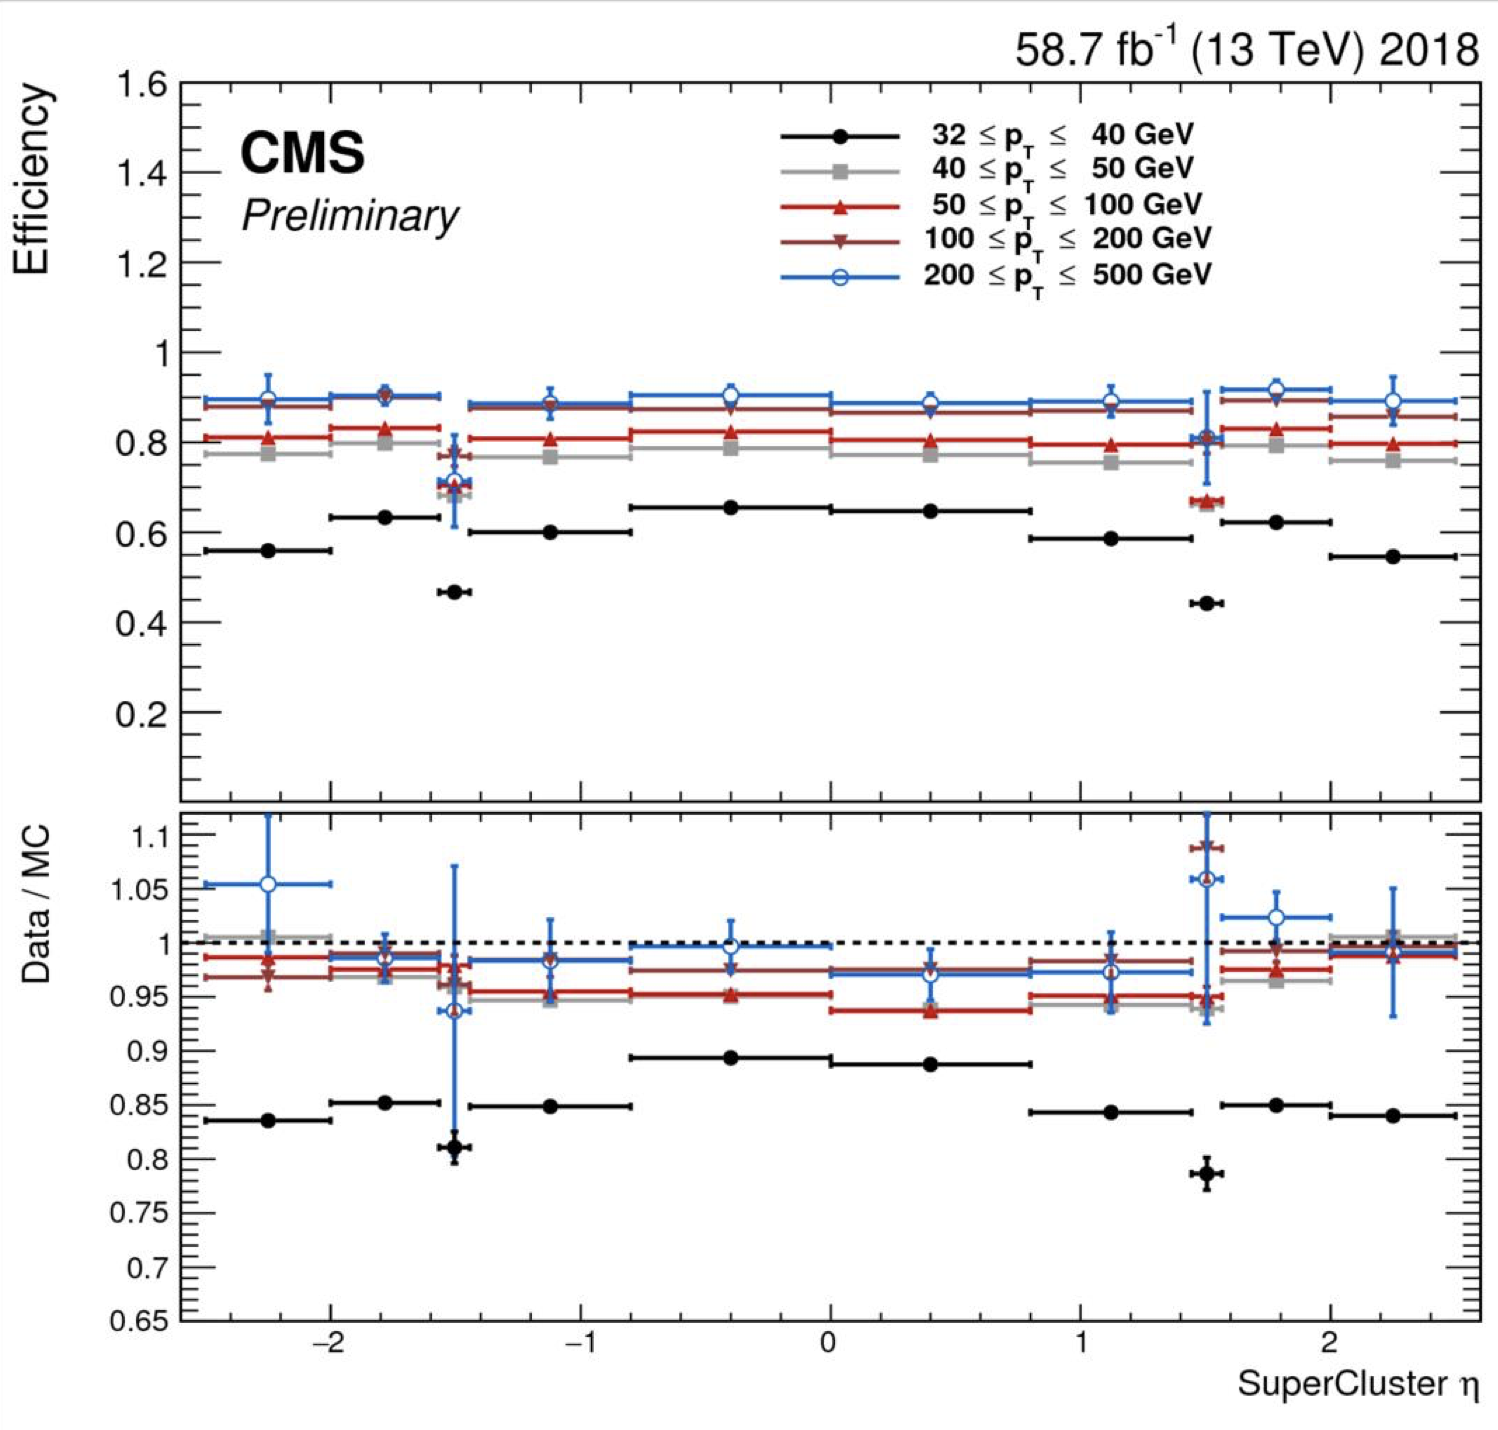
\includegraphics[width=1.0\textwidth]{figures/ch-8-scale-factors-and-corrections/electron_Ele32_WPTight_Gsf_efficiency_vsEta}
        \caption{Electron efficiency vs $|\eta|$ for single electron.}
        \label{fig:single_ele_32GeV_efficiency_vs_eta}
    \end{subfigure}
    \caption[Trigger efficiencies in data and the data/MC ratio for the electron in the single electron trigger with threshold $p_{T} > 32$ GeV in the data-taking year 2018, as functions of the electron $p_{T}$ (\textit{left}) and electron $|\eta|$ (\textit{right}).]{Trigger efficiencies in data, and the data/MC ratio for the electron in the single electron trigger with threshold $p_{T} > 32$ GeV in the data-taking year 2018, as functions of the electron $p_{T}$ (\textit{left}) and electron $|\eta|$ (\textit{right}) \cite{CMS-DP-2020-016}. In the plot vs. $p_{T}$, the region 1.442 $\leq |\eta| \leq$ 1.566 is not included as it corresponds to the transition between barrel and endcap parts of the ECAL.} 
\end{figure}


\subsection{$e\mu$ cross-trigger efficiencies}

The efficiencies of the electron and muons for the cross-trigger with leading muon used in the $e\mu$ channel are shown for data in 2016, 2017, and 2018 in Figures \ref{fig:ele_efficiency_vs_pT_emu} and \ref{fig:muon_efficiency_vs_eta_emu} \cite{CMS-DP-2019-025}. These efficiencies were measured centrally using a Tag and Probe in events with $Z$ to dileptons with the same flavour and opposite charge, where the tags are an isolated muon or electron, and the probe (offline) candidate is required to satisfy the same lepton selection as that of the tag candidate, be matched within $\Delta R < 0.1$ with a corresponding online trigger object, and also to pass the cross-trigger. The trigger efficiency is then:
\begin{equation}
    \text{Efficiency} = \frac{\text{Events passing lepton pair selections and probe passing trigger}}{\text{Events passing lepton pair selections}}
\end{equation}

\begin{figure}[h]
    \centering
    \begin{subfigure}{0.45\textwidth}
        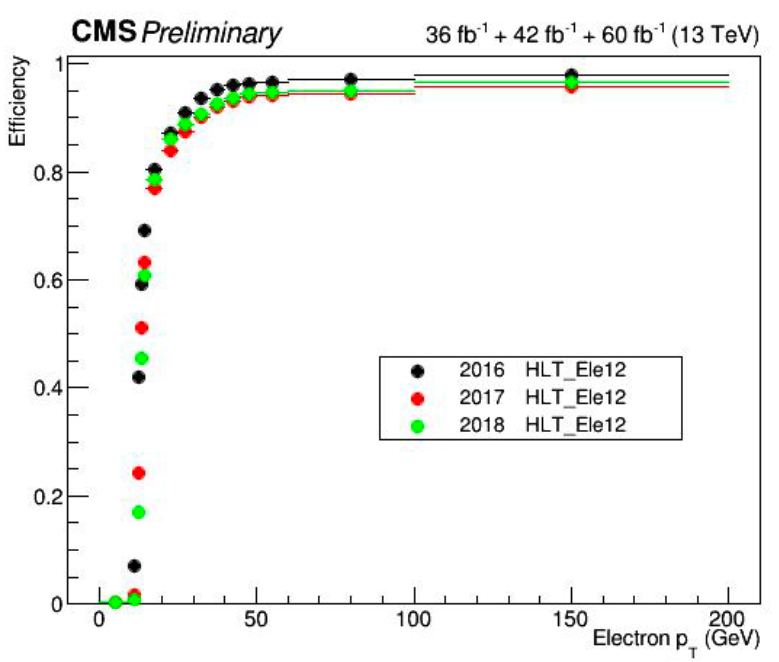
\includegraphics[width=1.0\textwidth]{figures/ch-8-scale-factors-and-corrections/ele_efficiency_vs_pT_emu_HLT_Mu23_TrkIsoVVL_Ele12_CaloIdL_TrackIdL_IsoVL_DZ.png}
        \caption{Electron efficiency vs. $p_{T}$.}
        \label{fig:ele_efficiency_vs_pT_emu}
    \end{subfigure}
    \hfill
    \begin{subfigure}{0.45\textwidth}
        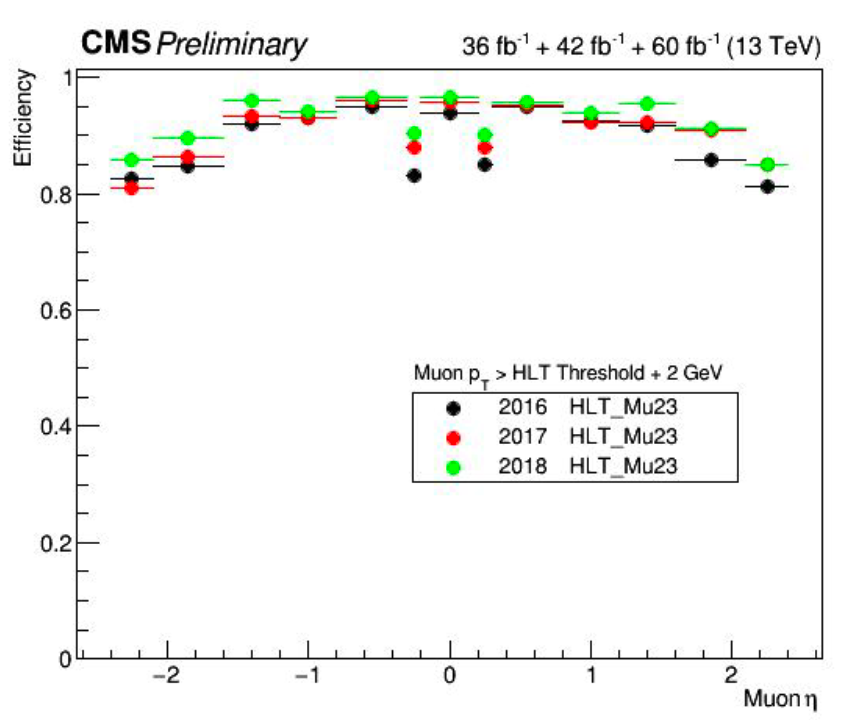
\includegraphics[width=1.0\textwidth]{figures/ch-8-scale-factors-and-corrections/muon_efficiency_vs_eta_emu_HLT_Mu23_TrkIsoVVL_Ele12_CaloIdL_TrackIdL_IsoVL_DZ.png}
        \caption{Muon efficiency vs. $\eta$.}
        \label{fig:muon_efficiency_vs_eta_emu}
    \end{subfigure}
    \caption[Efficiencies of the electron leg vs. $p_{T}$ (\textit{left}) and the muon log vs. $\eta$ (\textit{right}), for the HLT path with online thresholds of 12 GeV for the electron and 23 GeV for the muon, with the data-taking years 2016 through 2018 overlaid.]{Efficiencies of the electron leg vs. $p_{T}$ (\textit{left}) and the muon log vs. $\eta$ (\textit{right}), for the HLT path with online thresholds of 12 GeV for the electron and 23 GeV for the muon, for the data-taking years 2016 (\textit{black}), 2017 (\textit{red}), and 2018 (\textit{green}) \cite{CMS-DP-2019-025}.} 
\end{figure}


\section{Electrons and muons faking $\tau_{h}$: energy scales}

Energy scales for electrons misidentified as hadronic tau decays ($e$ faking $\tau_{h}$) are provided by the Tau POG, and were measured in the $e\tau_{h}$ channel with the visible invariant mass of the electron and hadronic tau system \cite{twiki_HiggsToTauTauWorkingLegacyRun2}. This energy scale is applied for $\tau_{h}$ with $p_{T} > 20$ GeV regardless of which DeepTau vs. electron working point was used. Values for 2018 are shown in Table \ref{table:electron-faking-tauh-FES-2018}.

% root -l TauFES_eta-dm_DeepTau2017v2p1VSe_2018ReReco.root 
\begin{table}[h]
    \centering
    \begin{tabular}{|c|c|}
    \hline
    \multicolumn{2}{|c|}{Electrons faking $\tau_{h}$ energy scale factor in 2018}      \\ \hline
    \hline
    Reconstructed decay mode of the fake $\tau_{h}$  & Central value and (up, down) shifts \\ \hline
    0   & 1.01362 (+0.00474, -0.00904) \\
    1   & 1.01945 (+0.01598, -0.01226) \\
    10  & 0.96903 (+0.0125, -0.03404) \\
    11 & 0.985 (+0.04309, -0.05499) \\ \hline
    \end{tabular}
    \caption[Energy scales and up/down systematic uncertainties applied to electrons misidentified as hadronic taus.]{Energy scales and up/down systematic uncertainties applied to electrons misidentified as hadronic taus for 2018, binned in decay mode of the fake $\tau_{h}$ \cite{twiki_HiggsToTauTauWorkingLegacyRun2}.}
    \label{table:electron-faking-tauh-FES-2018}
\end{table}

No nominal energy scale is applied for muons mis-reconstructed as $\tau_{h}$, and the uncertainty is treated as $\pm$ 1\% and uncorrelated in the reconstructed decay mode \cite{twiki_HiggsToTauTauWorkingLegacyRun2}. 

\section{Electrons and muons faking $\tau_{h}$: misidentification efficiencies}
Corrections on identification efficiencies are applied to genuine electrons and muons misidentified as $\tau$ to account for differences in data and MC.

The specific values depend on the vs. electron and vs. muon discriminator working points used. 
For misidentified $\mu \rightarrow \tau_{h}$, the scale factors are split into different $|\eta|$ regions, determined by the CMS muon and tracker detector geometries, as shown in Table \ref{table:tauIDeff_deepTau_vs_muon} for 2018 \cite{twiki_TAU_POG_tauidrecommendationforrun2}.


\begin{table}[h]
    \centering
    \begin{tabular}{|c|c|c|}
    \hline
    \multicolumn{3}{|c|}{Tau ID efficiency for DeepTau vs. muon WPs in 2018} \\ \hline
    \hline
    $|\eta|$  & Tight working point & VLoose working point \\ \hline
    (0.0, 0.2)     & 0.767 $\pm$ 0.127  & 0.954 $\pm$ 0.069  \\ \hline 
    (0.2, 0.6)     & 1.255 $\pm$ 0.258  & 1.009 $\pm$ 0.098  \\ \hline 
    (0.6, 1.0)     & 0.902 $\pm$ 0.203  & 1.029 $\pm$ 0.075 \\ \hline 
    (1.0, 1.45)    & 0.833 $\pm$ 0.415  & 0.928 $\pm$ 0.145\\ \hline
    (1.45, 2.0)    & 4.436 $\pm$ 0.814   & 5.000 $\pm$ 0.377 \\ \hline
    (2.0, 2.53)    & 1.000 $\pm$ 0.000         & 1.000 $\pm$ 0.000\\ \hline
    \end{tabular}
    \caption[Tau mis-identification efficiency for the DeepTau Tight and Very Loose (VLoose) working points vs. muons in 2018.]{Tau mis-identification efficiency for the DeepTau Tight and Very Loose (VLoose) working points vs. muons in 2018, binned in the muon $|\eta|$ \cite{twiki_TAU_POG_tauidrecommendationforrun2}.}
    \label{table:tauIDeff_deepTau_vs_muon}
\end{table}

For misidentified $e \rightarrow \tau_{h}$, the scale factors are split into barrel and endcap regions, dictated by the ECAL detector geometry, as shown in Table \ref{table:tauIDeff_deepTau_vs_electron} for 2018.

% root -l /Users/stephaniekwan/Dropbox/Princeton_G6/TauIDSFs/data/TauID_SF_eta_DeepTau2017v2p1VSe_2018ReReco.root 
\begin{table}[h]
    \centering
    \begin{tabular}{|c|c|c|}
    \hline
    \multicolumn{3}{|c|}{Tau ID efficiency for DeepTau vs. electron WPs in 2018} \\ \hline
    \hline
    $|\eta|$  & Tight working point & VLoose working point \\ \hline
    (0.0, 0.73)     & 1.47 $\pm$ 0.27  & 0.95 $\pm$ 0.07  \\ \hline 
    (0.73, 1.509)   & 1.509 $\pm$ 0.0  & 1.00 $\pm$ 0.0  \\ \hline 
    (1.509, 1.929)  & 1.929 $\pm$ 0.2  & 0.86 $\pm$ 0.1 \\ \hline 
    (1.929, 2.683)  & 2.683 $\pm$ 0.9  & 2.68 $\pm$ 0.0 \\ \hline
    \end{tabular}
    \caption[Tau mis-identification efficiency for the DeepTau Tight and Very Loose (VLoose) working points vs. electrons in 2018.]{Tau mis-identification efficiency for the DeepTau Tight and Very Loose (VLoose) working points vs. electrons in 2018, binned in the electron $|\eta|$ \cite{twiki_TAU_POG_tauidrecommendationforrun2}.}
    \label{table:tauIDeff_deepTau_vs_electron}
\end{table}


\section{Electron ID and tracking efficiency}
Scale factors are applied to MC to correct for differences between MC and data in the performance of electron identification (ID) and tracking.

Electron and photon identification, as discussed earlier, use variables with good signal vs. background discrimination power such as lateral shower shape and ratio of energy deposited in the HCAL to energy deposited in the ECAL at the position of the electron. The cut-based electron identification efficiencies in data and ratio of efficiencies in data to MC are shown in Fig. \ref{fig:electron_MVA_ID_efficiency} for the multivariate analysis (MVA) identification working point. 

The tracking efficiencies in data and the data/MC ratio are shown in Fig. \ref{fig:electron_GSF_tracking_efficiency} for the Gaussian-sum filter (GSF) tracking \cite{CMS-DP-2020-037}. 

\begin{figure}[h]
    \centering
    \begin{subfigure}{0.45\textwidth}
        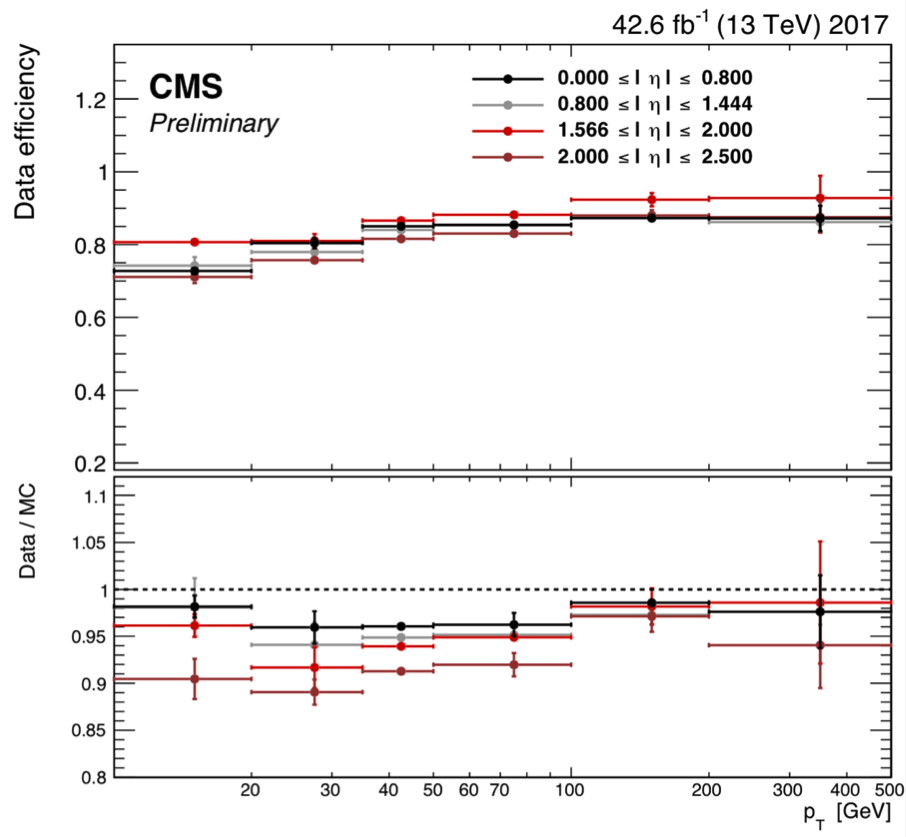
\includegraphics[width=1.0\textwidth]{figures/ch-8-scale-factors-and-corrections/electron_MVA_90wp_identification_efficiency}
        \caption{Electron MVA ID.}
        \label{fig:electron_MVA_ID_efficiency}
    \end{subfigure}
    \hfill
    \begin{subfigure}{0.45\textwidth}
        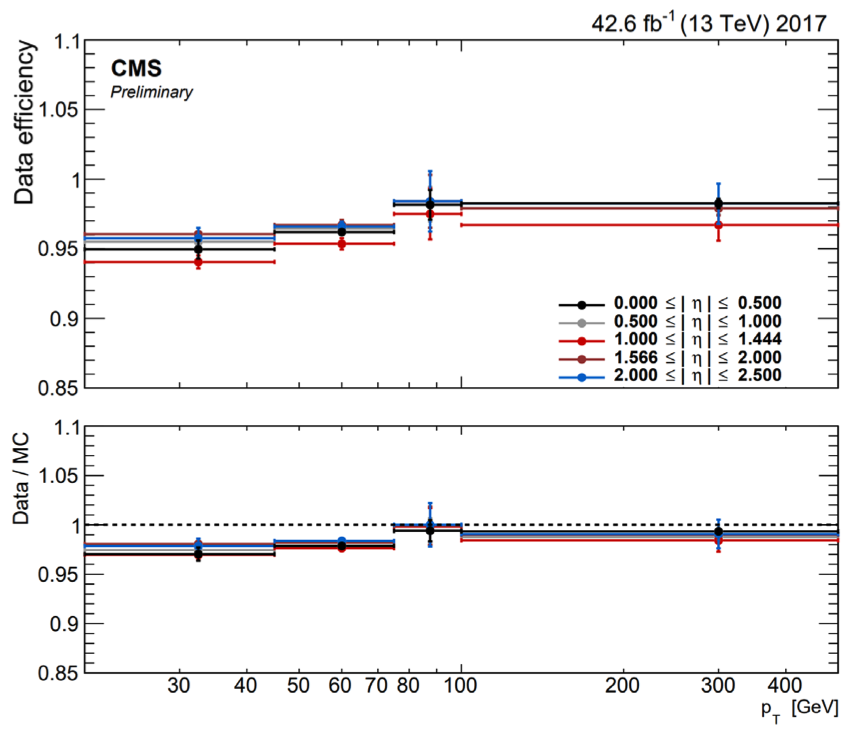
\includegraphics[width=1.0\textwidth]{figures/ch-8-scale-factors-and-corrections/electron_gsf_tracking_efficiency}
        \caption{Electron GSF tracking.}
        \label{fig:electron_GSF_tracking_efficiency}
    \end{subfigure}
    \caption[Efficiencies in data (\textit{top panels}) and the ratio of efficiencies in data/MC (\textit{bottom panels}), for the electron multivariate analysis (MVA) identification (\textit{left}) and for the Gaussian-sum filter (GSF) tracking (\textit{right}).]{Efficiencies in data (\textit{top panels}) and the ratio of efficiencies in data/MC (\textit{bottom panels}), for the electron multivariate analysis (MVA) identification (\textit{left}) and for the Gaussian-sum filter (GSF) tracking (\textit{right}) \cite{CMS-DP-2020-037}. Error bars represent statistical and systematic uncertainties.} 
\end{figure}


\section{Muon ID, isolation, and tracking efficiencies}
Scale factors are applied to MC to correct for differences between MC and data in the performance of muon identification, isolation, and tracking, as detailed below.

The efficiencies for muon identification measured in 2015 data and MC simulation are shown in Figures \ref{fig:muon_looseID_efficiency} and \ref{fig:muon_tightID_efficiency} for the loose ID and tight ID respectively \cite{CMS-MUO-16-001}. The loose ID is chosen such that efficiency exceeds 99\% over the full $\eta$ range, and the data and simulation agree to within 1\%. The tight ID is chosen such that efficiency varies between 95\% and 99\% as a function of $\eta$, and the data and simulation agree to within 1-3\%. The muon identification working point used in this analysis is the medium ID, which has an efficiency of 98\% for all $\eta$ and an agreement within 1-2\% \cite{CMS-MUO-16-001}. 

\begin{figure}[h]
    \centering
    \begin{subfigure}{0.45\textwidth}
        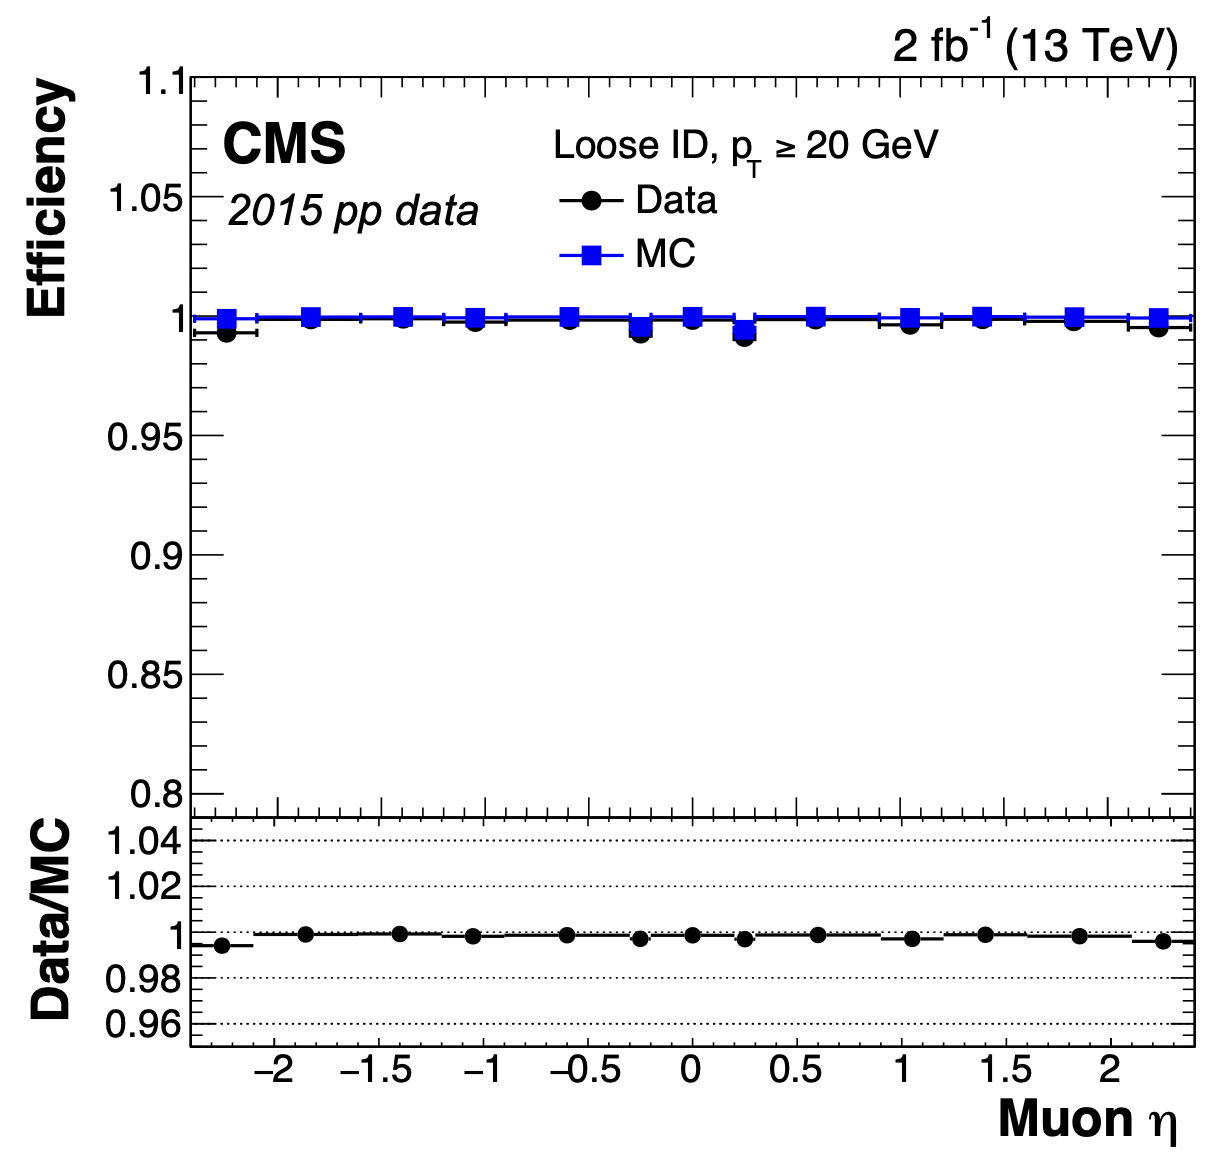
\includegraphics[width=1.0\textwidth]{figures/ch-8-scale-factors-and-corrections/muon_efficiency_looseID}
        \caption{Muon efficiency isolation vs $p_{T}$.}
        \label{fig:muon_looseID_efficiency}
    \end{subfigure}
    \hfill
    \begin{subfigure}{0.45\textwidth}
        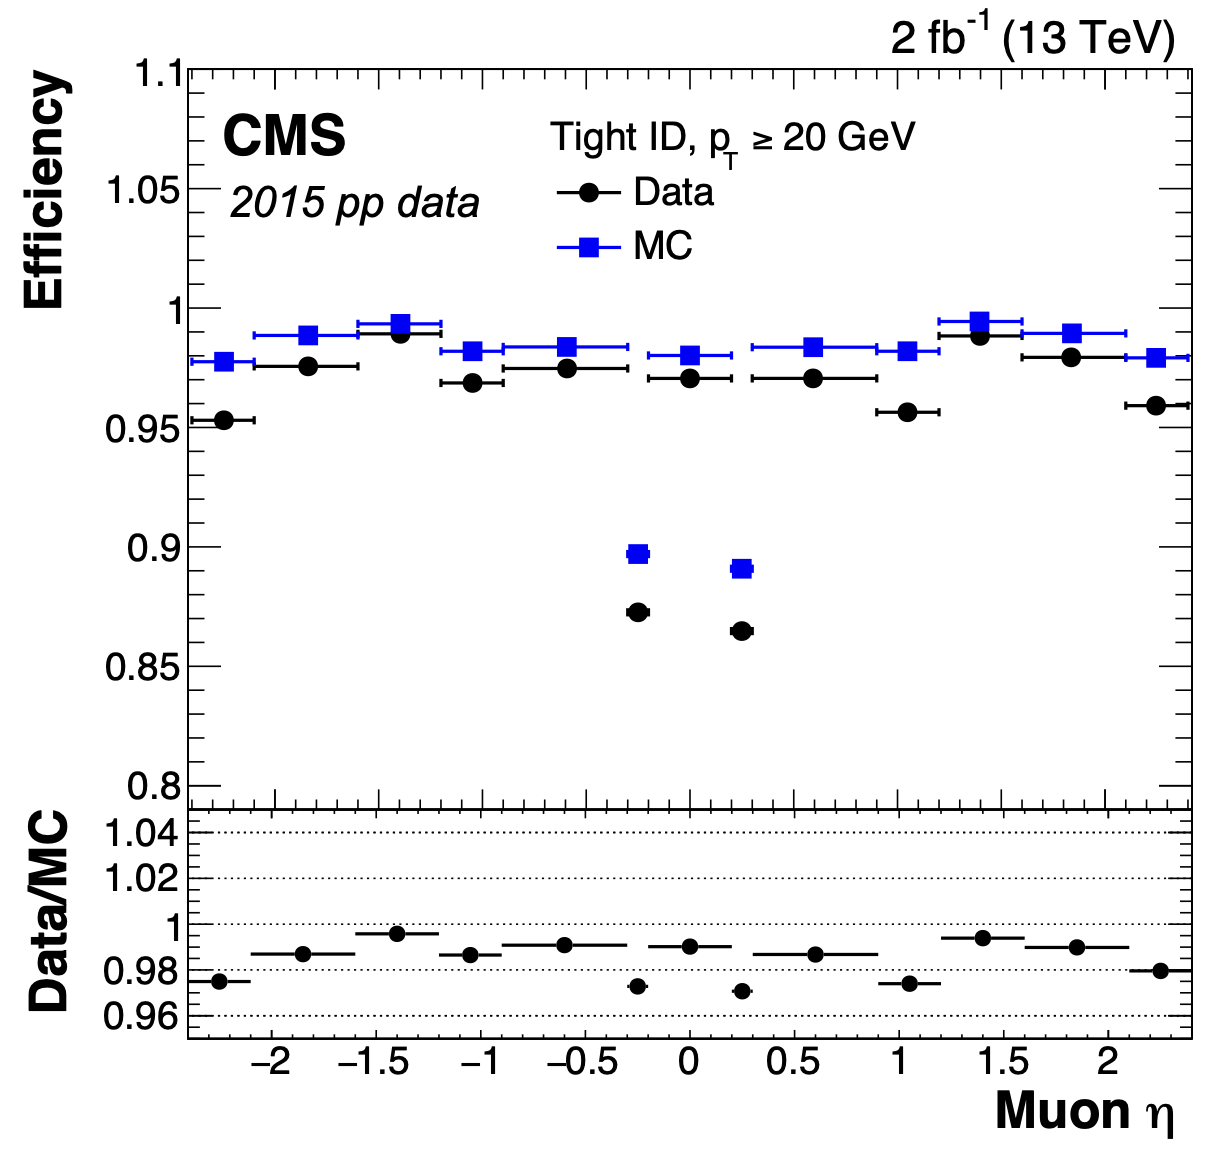
\includegraphics[width=1.0\textwidth]{figures/ch-8-scale-factors-and-corrections/muon_efficiency_tightID}
        \caption{Muon isolation efficiency vs. $|\eta|$.}
        \label{fig:muon_tightID_efficiency}
    \end{subfigure}
    \caption[Muon identification efficiencies in 2015 data and MC as a function of the muon $p_{T}$ for the loose ID (\textit{left}) and tight ID (\textit{right}) working points.]{Muon identification efficiencies in 2015 data and MC as a function of the muon $p_{T}$ for the loose ID (\textit{left}) and tight ID (\textit{right}) working points \cite{CMS-MUO-16-001}.} 
\end{figure}

The efficiencies in data for the muon isolation, as measured in Level-3 muons (muons in one of the final stages of reconstruction in the HLT), as a function of the muon $p_{T}$ and $|\eta|$ are shown in Figures \ref{fig:muon_isolation_efficiency_vsPt} and \ref{fig:muon_isolation_efficiency_vsEta} \cite{CMS-MUO-16-001}. The HLT muon reconstruction consists of two steps: Level-2 (L2), where the muon is reconstructed in the muon subdetectors only, and Level-3 (L3) which is a global fit of tracker and muon hits (i.e. the global muon reconstruction as described in Section \ref{section:ch-5-muon-reconstruction}) \cite{Verwilligen-proceedings-2016}.

\begin{figure}[h]
    \centering
    \begin{subfigure}{0.45\textwidth}
        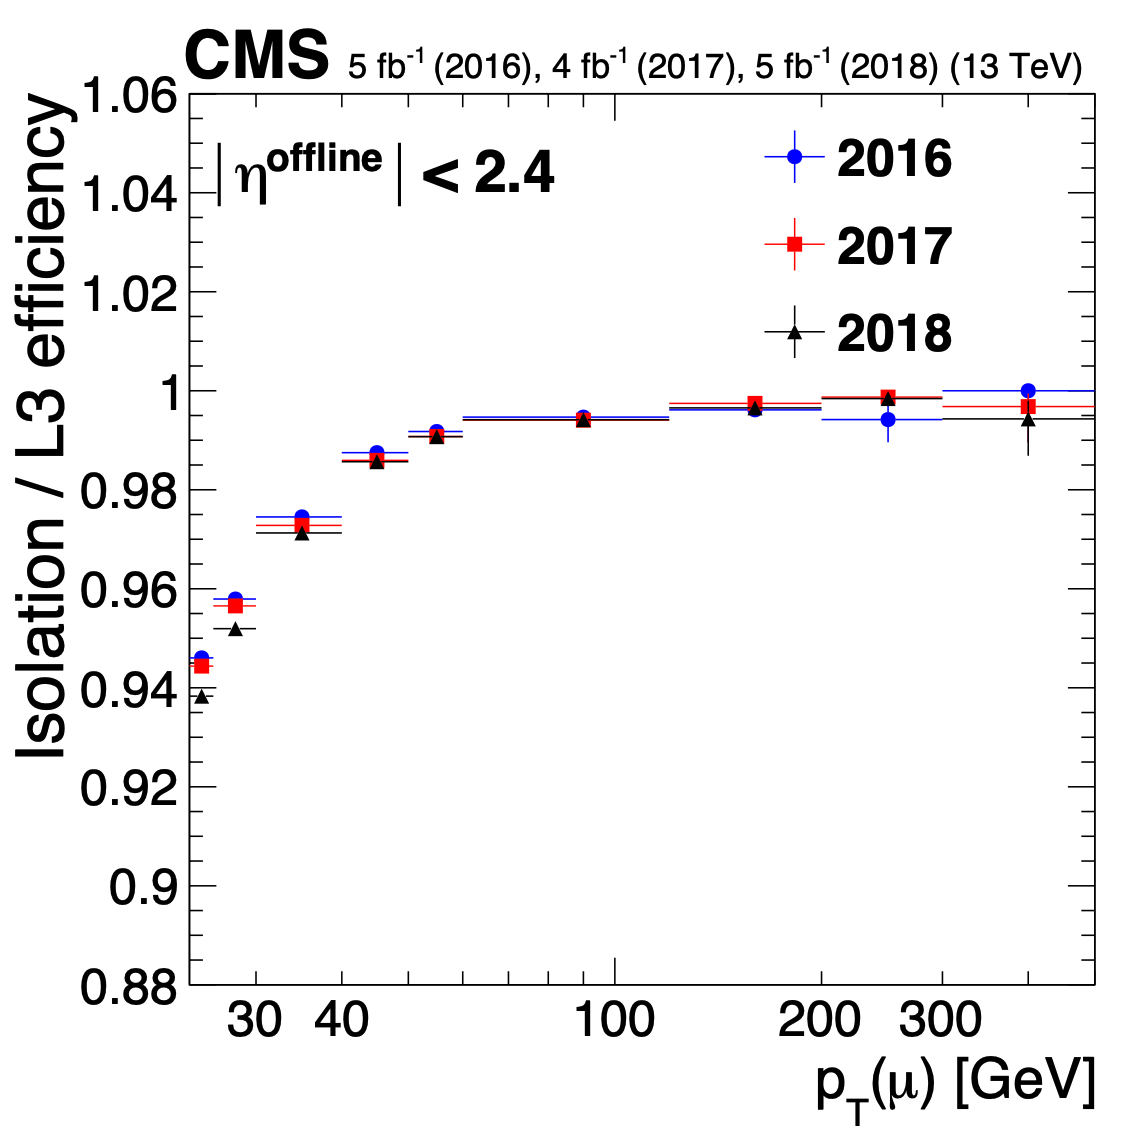
\includegraphics[width=1.0\textwidth]{figures/ch-8-scale-factors-and-corrections/muon_efficiency_isolation_vsPt}
        \caption{Muon efficiency isolation vs $p_{T}$.}
        \label{fig:muon_isolation_efficiency_vsPt}
    \end{subfigure}
    \hfill
    \begin{subfigure}{0.45\textwidth}
        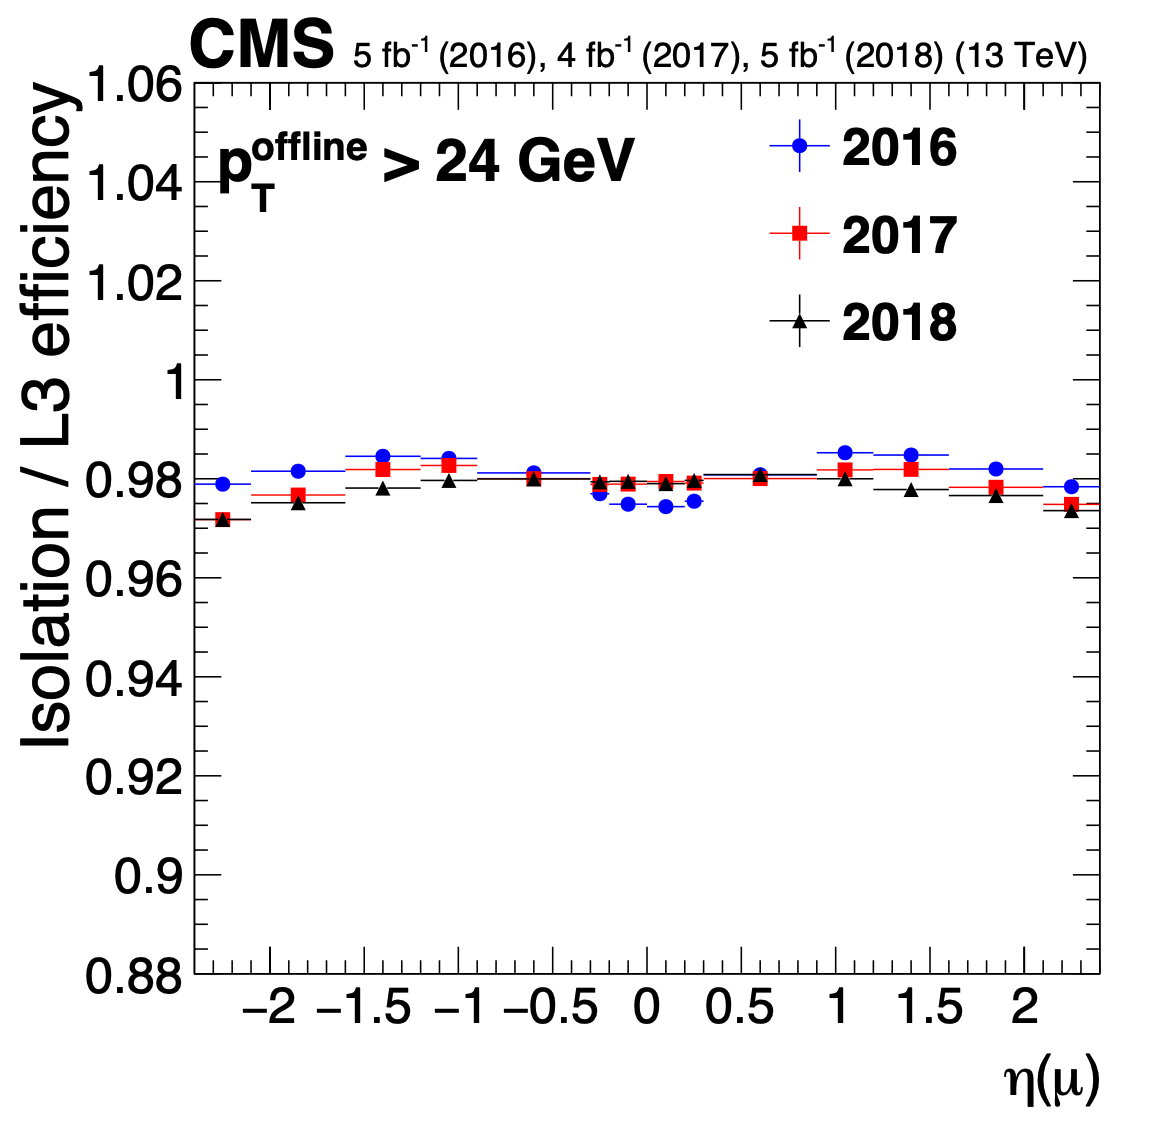
\includegraphics[width=1.0\textwidth]{figures/ch-8-scale-factors-and-corrections/muon_efficiency_isolation_vsEta}
        \caption{Muon isolation efficiency vs. $|\eta|$.}
        \label{fig:muon_isolation_efficiency_vsEta}
    \end{subfigure}
    \caption[Muon isolation efficiencies in Run-2 data as a function of the muon $p_{T}$ (\textit{left}) and $|\eta|$ (\textit{right}).]{Muon isolation efficiencies in Run-2 data with respect to Level-3 muons (one of the final stages of HLT muon reconstruction) as a function of the muon $p_{T}$ (\textit{left}) and $|\eta|$ (\textit{right}) \cite{CMS-MUO-16-001}.} 
\end{figure}

The muon tracking efficiencies as a function of $|\eta|$ for standalone muons (i.e. tracks from only the muon system, i.e. DT, CSC, and RPC, as discussed in Section \ref{section:ch-5-muon-reconstruction}), is shown for data and simulated Drell-Yan samples in Fig. \ref{fig:muon_tracking_efficiency} \cite{CMS-DP-2020-035}. 

\begin{figure}[h]
    \centering
    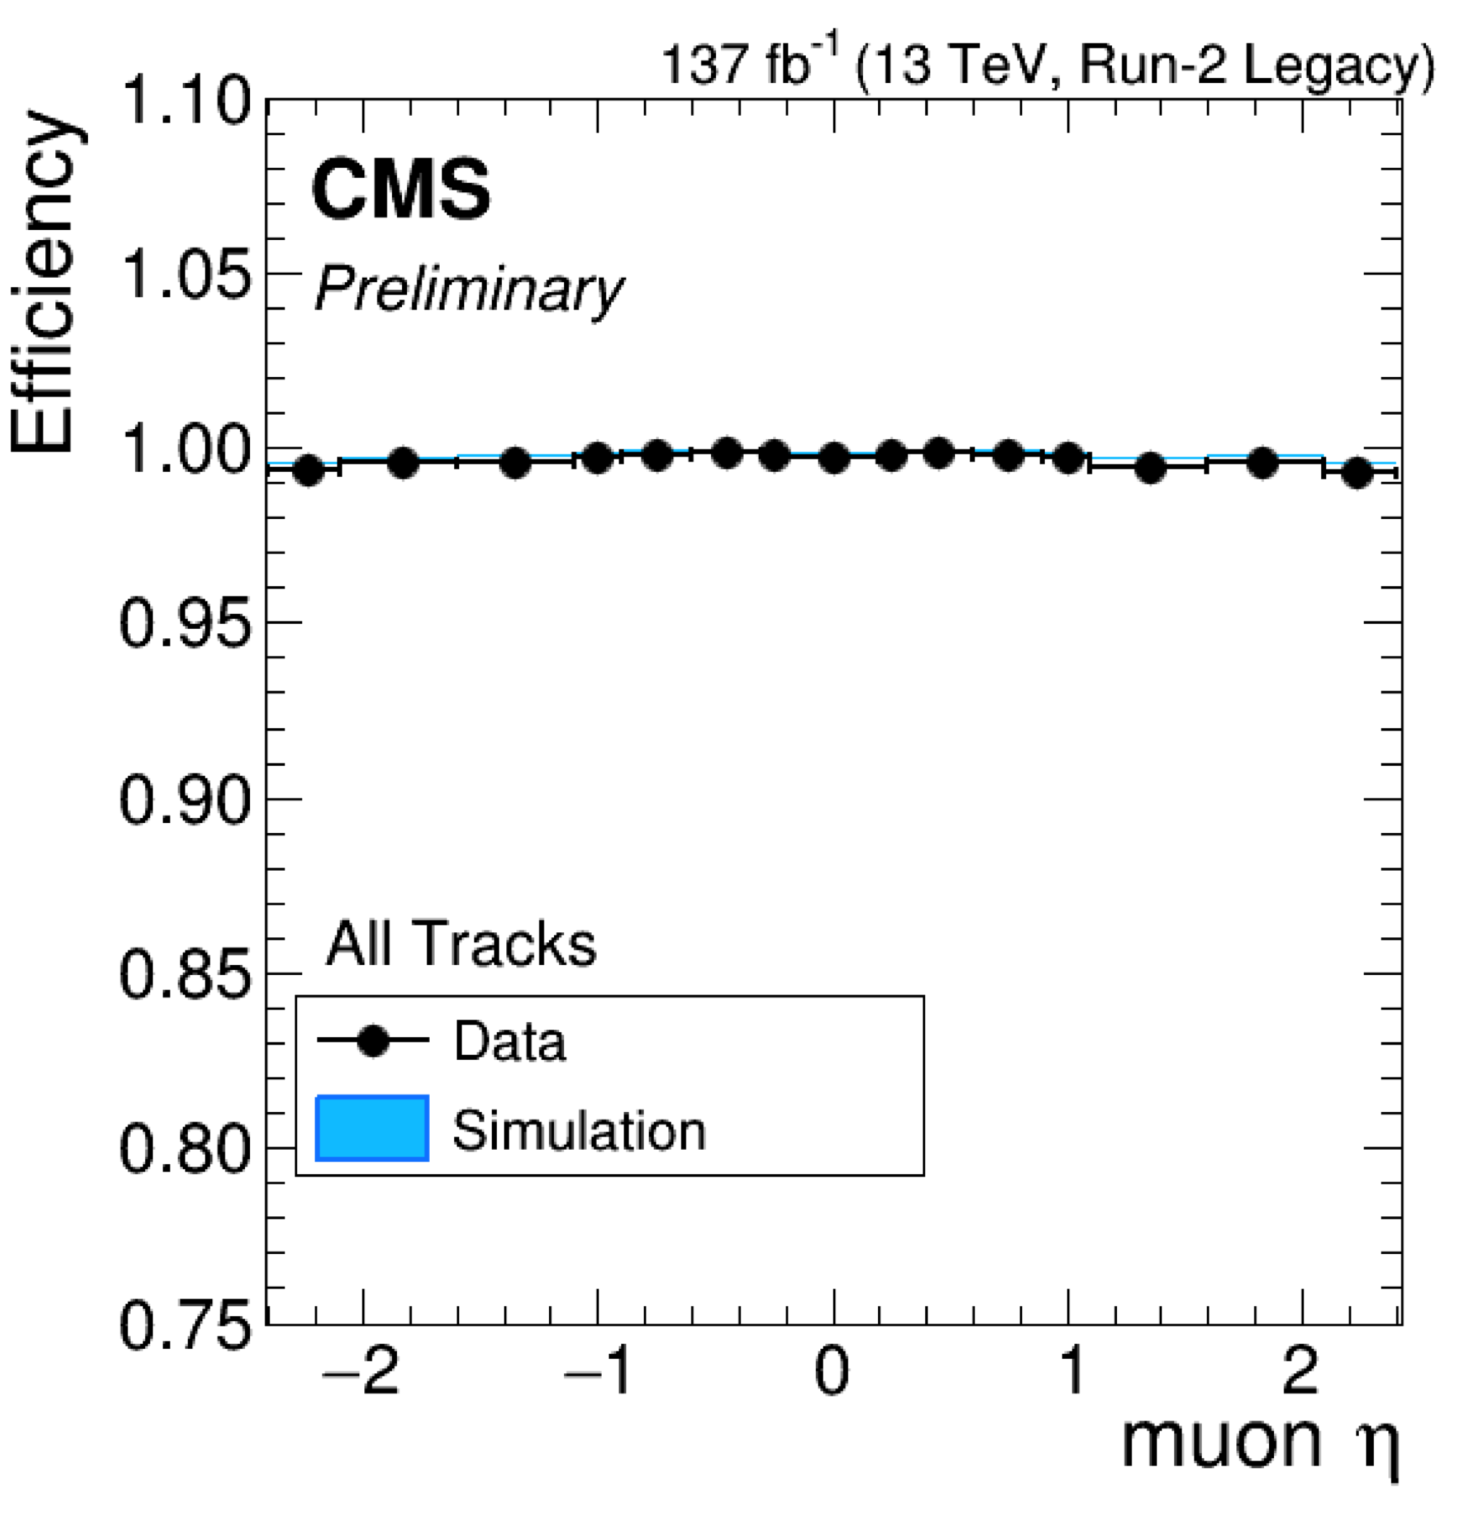
\includegraphics[width=8cm]{figures/ch-8-scale-factors-and-corrections/muon_tracking_efficiency}
    \caption[Muon tracking efficiencies as a function of $|\eta|$ for standalone muons in Run-2 data (\textit{black}) and Drell-Yan (\textit{blue}) MC simulation.]{Muon tracking efficiencies as a function of $|\eta|$ for standalone muons in Run-2 data (\textit{black}) and Drell-Yan MC simulation (\textit{blue}) \cite{CMS-DP-2020-035}. All Tracks refers to tracks which exploit the presence of muon candidates in the muon system to seed the track reconstruction in the inner tracker, in contrast to tracks that use tracker-only hits for seeding. Uncertainties shown are statistical.}
    \label{fig:muon_tracking_efficiency}
\end{figure}

    

\section{Recoil corrections}
\label{sec:ch-8-recoil-corrections}
In proton-proton collisions, W and Z bosons are predominantly produced through quark-antiquark annihilation. Higher-order processes can induce radiated quarks or gluons that recoil against the boson, imparting a non-zero transverse momentum to the boson \cite{2009-Tevatron-recoil-correction}. Recoil corrections accounting for this effect are applied to samples with W+jets, Z+jets, and Higgs bosons \cite{twiki_HiggsToTauTauWorkingLegacyRun2}. The corrections are performed on the vectorial difference between the measured missing transverse momentum and the total transverse momentum of neutrinos originating from the decay of the W, Z, or Higgs boson. This vector is projected onto the axes parallel and orthogonal to the boson $p_{T}$. This vector, and the resulting correction to use, is measured in $Z \rightarrow \mu\mu$ events, since these events have leptonic recoil that do not contain neutrinos, allowing the 4-vector of the Z boson to be be measured precisely. The corrections are binned in generator-level $p_{T}$ of the parent boson and also the number of jets in the event.

\section{Drell-Yan corrections}
The Z boson transverse momentum distribution disagrees between leading-order (LO) simulations and data in a $Z \rightarrow \mu\mu$ control region with at least one b-tag jet \cite{CMS-HIG-17-024}. Per-event weights derived by the 2016 data-only version of this analysis \cite{CMS-HIG-17-024} are applied to $Z \rightarrow \tau\tau / \ell \ell$ events, as a function of the generator-level Z boson $p_{T}$ to provide better matching of MC to data.

\section{Pileup reweighing}
Reweighing is performed to rescale MC events to account for differences between MC and data, in the distribution of the pileup (number of additional proton-proton interactions per bunch crossing). A tool for calculating the pileup reweighing for the MC samples used is provided centrally by the Luminosity POG \cite{twiki_LUMI_POG_recommendation}.

\section{Pre-firing corrections}
In 2016 and 2017 data-taking, a gradual timing shift of ECAL was not properly propagated to L1 trigger primitives (TPs), resulting in a large fraction of high $\eta$ TPs being incorrectly associated with the previous bunch crossing. L1 trigger rules prevent two consecutive bunch crossings from firing, causing events to be rejected if significant ECAL energy was deposited in $2.0 < |\eta| 3.0$. To account for this issue, MC simulations for 2016 and 2017 are corrected using an event-dependent weight. Embedded samples are not corrected \cite{CMS-HIG-19-010}.

\section{Top $p_{T}$ spectrum reweighing}
In Run-1 and Run-2 it was observed that the $p_{T}$ spectra of top quarks in $t\bar{t}$ data was significantly softer than those predicted by MC simulations \cite{twiki_Top_pt_reweighing}. Possible sources of this discrepancy are higher order QCD and/or electroweak corrections, and non-resonant production of $t\bar{t}$-like final states. To account for this, corrections derived from Run-2 data by the Top Physics Analysis Group (PAG) are applied to the $p_{T}$ of the top and anti-top quarks in MC simulations, computed as a function of their generator-level $p_{T}$ \cite{twiki_Top_pt_reweighing}.

\section{B-tagging efficiency}
In order to predict correct b-tagging discriminant distributions and event yields in data, the weight of selected MC events is reweighed according to recommendations by the BTV POG \cite{twiki_btag_SF_methods}. The reweighing depends on the jet $p_{T}$, $\eta$, and the b-tagging discriminant. In this method, there is no migration of events from one b-tag multiplicity bin to another.

\section{Jet energy resolution and jet energy smearing}
Calibration of jet energies, i.e. ensuring that the energy and momentum of the reconstructed jet matches that of the quark/gluon-initiated jet, is a challenging task due to time-dependent changes in the detector response and calibration and high pileup \cite{CMS-JME-13-004} \cite{proceedings-Agarwal:2022txa}. Jet calibration is done via jet energy corrections (JECs) applied to the $p_{T}$ of jets in MC samples, accounting successively for the effects of pileup, uniformity of the detector response, and residual data-simulation jet energy scale differences \cite{twiki_JetResolution_JEC}. Typical jet energy resolutions reported at $\sqrt{s} = 8$ TeV in the central rapidities are 15-20\% at 30 GeV and about 10\% at 100 GeV \cite{CMS-JME-13-004}. Jet energy corrections are also propagated to the missing transverse energy.

Measurements show that the jet energy resolution (JER) in data is worse than in simulation, and so the jets in MC need to be smeared to describe the data. JER corrections are applied after JEC on MC simulations, and adjust the width of the $p_{T}$ distribution based on pileup, jet size, and jet flavour \cite{twiki_JetResolution_JER}. Tools for applying JEC and JER are provided centrally by the JER Corrections group. 

\chapter{Background estimation}
This section describes methods used to estimate sources of background from Standard Model processses in the search for $h \rightarrow aa \rightarrow bb\tau\tau$. Similar background estimation methods are being used for the $h \rightarrow a_1 a_2$ analysis. The background contributions directly taken from MC are described first, followed by backgrounds estimated from data-driven methods to produce sufficient statistics in the signal region.

\section{Z+jets}

A major source of background for $\tau\tau$ analyses is the Drell-Yan (DY) process (Z+jets). The Z boson decays to $\tau\tau/ \mu\mu/ ee$ with equal probability of 3.4\% each, with the dominant decay modes being to hadrons (around 70\%) and neutrinos (invisible) (20\%) \cite{workman_review_2022}. 

The Drell-Yan contribution with genuine taus, Z $\rightarrow \tau\tau$, is estimated using embedded samples, described in Section \ref{sec:embedded-samples}. To avoid double-counting between embedded and MC samples, in all MC samples, events with legs that originated from genuine $\tau$ are discarded.

The other decays of the Z, Z $\rightarrow ee$ and Z $\rightarrow \mu\mu$, are estimated from MC simulation, and are hereafter referred to as simply the Drell-Yan background. These MC samples are generated to leading order (LO) with different numbers of jets (jet multiplicity) in the matrix element: Z+1 jet, Z+2jets, Z+3 jets, Z+4 jets, and inclusive Z+jets. The cross-sections of the samples with $\geq 1$ jets are normalized to next-to-NLO (NNLO) in QCD.

For the inclusive Drell-Yan sample, two samples are used with different thresholds for the di-lepton invariant mass ($m_{\ell}$) at the generator level: one with $m_{\ell\ell} > 50$ GeV and the other with $10 < m_{\ell\ell} < 50$. 

\section{W+jets}

The dominant W boson decay modes are to hadrons (67.4\%), $e + \nu_e$ (10.7\%), $\mu + \nu_\mu$ (10.6\%), and $\tau + \nu_\tau$ (11.4\%) \cite{workman_review_2022}.
The W+jets background is estimated from MC simulation. Similarly to the Z+jets, the W+jets samples are generated with different jet multiplicities in the matrix element. LO samples are used for greater statistics and are normalized to NNLO cross sections. 

\section{$t\bar{t}$ + jets}
In hadron collisions, top quarks are produced singly with the weak interaction, or in pairs via the strong interaction, with interference between these leading-order processes possible in higher orders of the perturbation theory. 
The top quark is the heaviest fermion in the Standard Model and has a short lifetime ($\sim 10^{-25}$ s), decaying without hadronization into a bottom quark and a W boson \cite{workman_review_2022}, with the decay modes of the W boson as listed in the previous section. With two top quarks, the final states of the two resulting W bosons can be described as fully leptonic, semileptonic, and fully hadronic. These three final states are modeled separately with MC simulation in 2018 and 2017, while for 2016 the sample used is inclusive.

\section{Single top}
% https://cms.cern/news/measurement-t-channel-single-top-quark-production-rates-pp-collisions-7-tev
There are three main production modes of the single top in $pp$ collisions \cite{CMS-CR-2018-185}: the exchange of a virtual W boson ($t$ channel), the production and decay of a virtual W boson ($s$ channel), and the associated production of a top quark and W boson ($tW$, or W-associated) channel. As the $s$ channel process is rare and only 3\% of the total production, the dominant production mode of the $t-channel$ and the $tW$ production are considered and modeled with MC. 

\section{Diboson}

In $pp$ collisions, the production of dibosons (pairs of electroweak gauge bosons, i.e. WW, WZ, and ZZ) is dominated by quark-antiquark annihilation, with a small contribution from gluon-gluon interaction \cite{CMS-SMP-20-012}. MC is used to model the pair production and decays of VV to $2\ell 2\nu$, WZ to $2q 2\ell$ and $3 \ell \nu$, and ZZ to $4\ell$ and $2q 2\ell$ ($q$ being quarks and $\ell$ being leptons).

\section{Standard Model Higgs}

MC is used to simulate backgrounds from major production modes of the Standard Model 125 GeV Higgs boson: gluon-gluon fusion (ggH), vector boson fusion (VBF), associated production with a W or Z (WH, ZH), and associated production with a top pair (ttH) (see Fig. \ref{fig:higgs-boson-production-modes} for leading-order diagrams). For these production modes, samples with the Higgs decaying to $\tau\tau$ or to $WW$ are used. Samples made with higher-order diagrams for WH and ZH that include the production of a jet, with the Higgs decaying to WW, are also used.

\begin{figure}[ht]
    \centering
    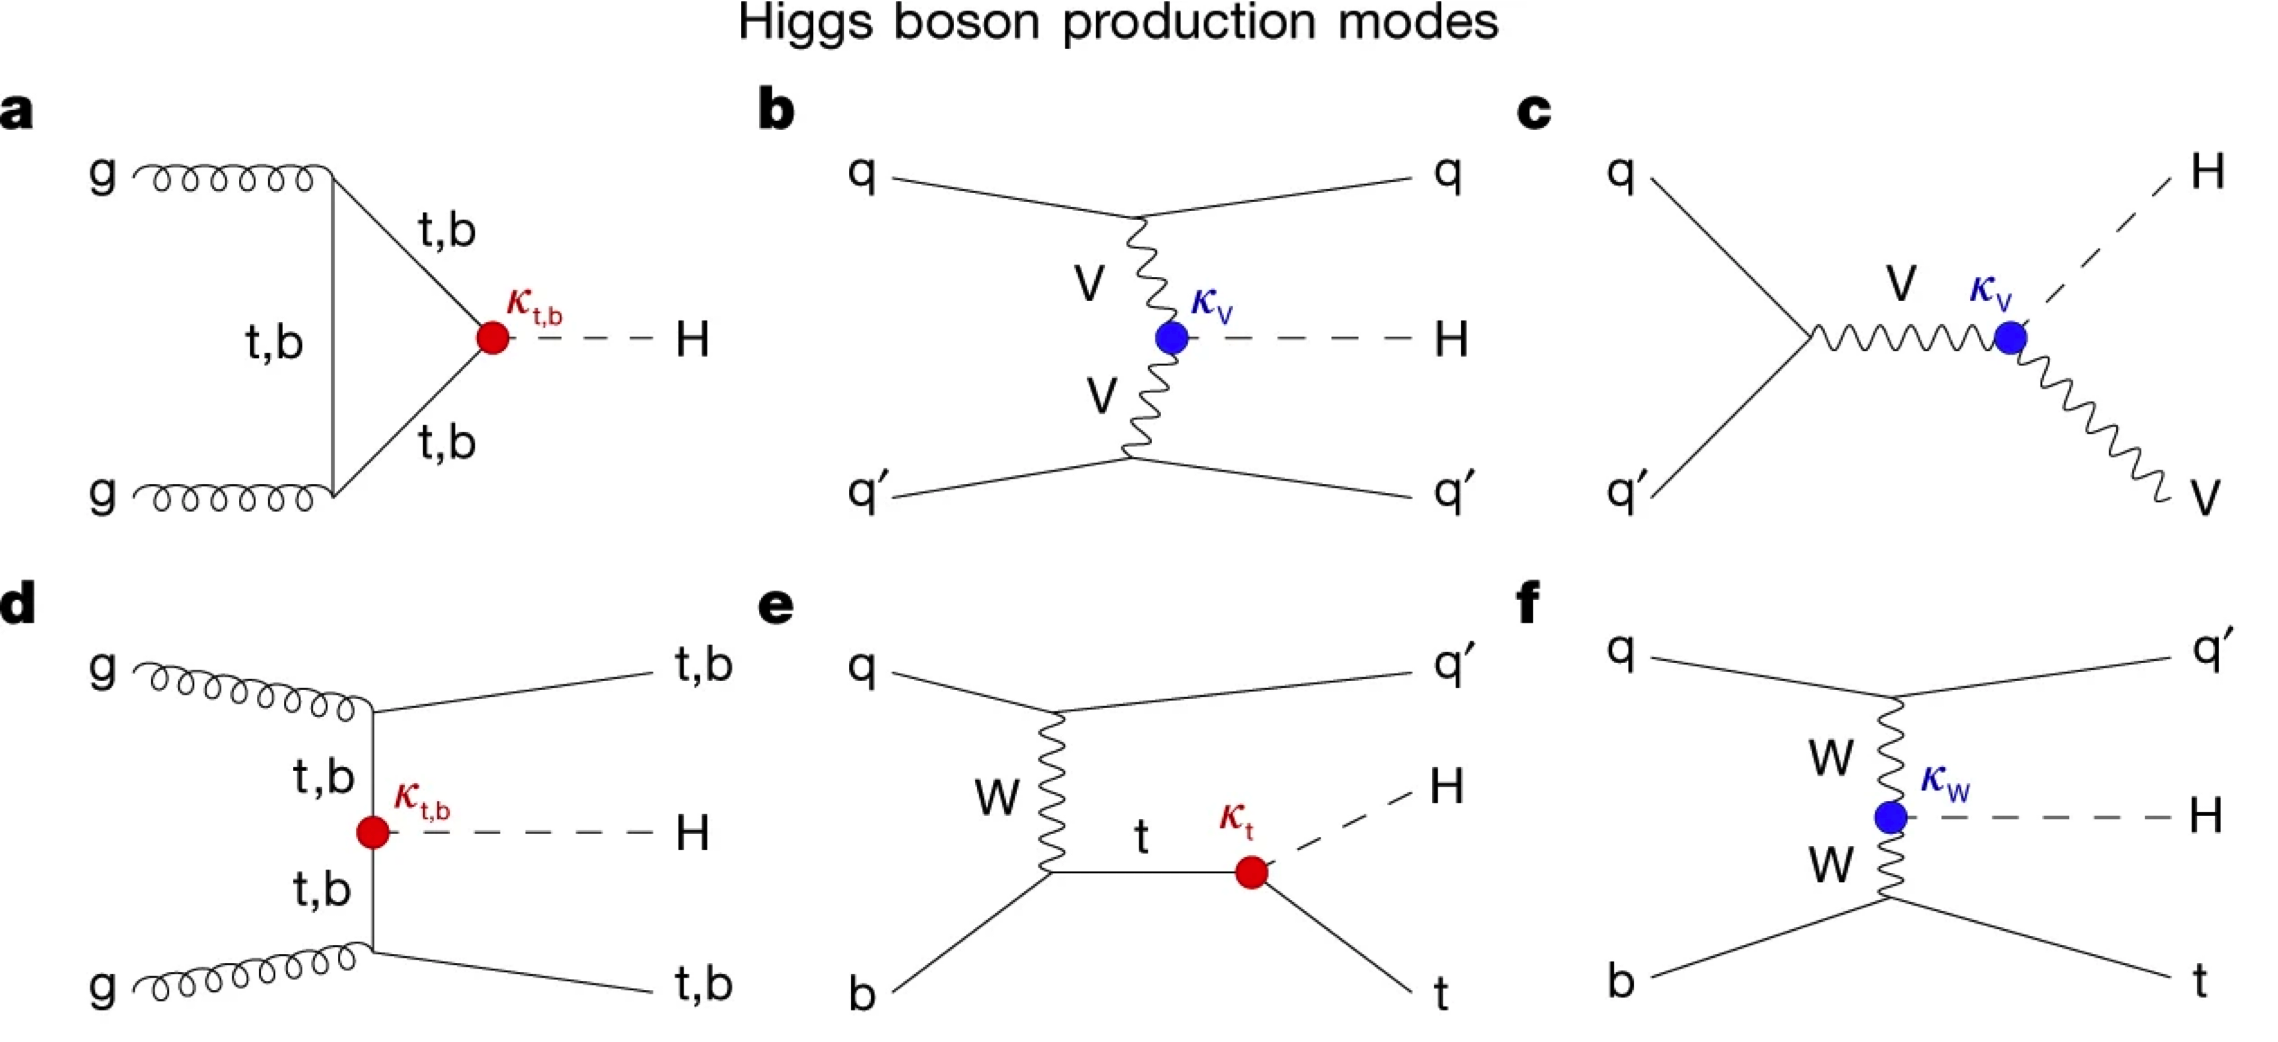
\includegraphics[width=15cm]{figures/ch-9-background-estimation/higgs-boson-production-modes.png}
    \caption[Leading-order Feynman diagrams of Higgs production.]{Leading-order Feynman diagrams of Higgs production from \cite{CMS-HIG-22-001}, in ggH (\textit{a}) and vector boson fusion (VBF; \textit{b}), associated production with a W or Z (V) boson (VH; \textit{c}), associated production with a top or bottom quark pair (ttH or bbH); \textit{d}, and associated production with a single top quark (tH; \textit{e, f}).} 

     \label{fig:higgs-boson-production-modes}
\end{figure}

\section{Jet faking $\tau_{h}$ background for the $\mu\tau_{h}$ and $e\tau_{h}$ channels}


\chapter{Event categorization}
\label{chapter:ch-10:event-categorization}
\section{B-tag jet multiplicity}
The increased statistics of the full Run-2 dataset enables the separation of events into events with exactly 1 b-tag jet and events with greater than 1 b-tag jet. Further event categorization is performed with deep neural networks (DNNs) described below. The DNNs  are used only for separating events into signal and control regions in the 1 b-tag and 2 b-tag jets scenarios. The final results are extracted from the statistical fitting to the mass of the $\tau\tau$, $m_{\tau\tau}$.

\section{DNN-based event categorization}
A brief overview of the DNN-based event categorization is given below with a focus on the physics aspects, with full details of the machine learning training in \cite{CMS-HIG-22-007} and associated documentation.

\subsubsection{Training samples}
Neural networks for event categorization are trained for each of the $\mu\tau_{h}$, $e\tau_{h}$, and $e\mu$ channels, for 1 and 2 b-tag jets, giving $3 \times 2 = 6$ networks in total. In the training, the signal is taken to be all of the possible pseudoscalar mass $m_{a}$ hypotheses together. The backgrounds for each DNN are taken to be a representative combination of the three major backgrounds: $Z \rightarrow \tau\tau$, $t\bar{t}$+jets, and fake backgrounds. The proportions of each background for each channel and b-tag jet multiplicity are taken from the yields in the $m_{\tau\tau}$ distribution. For instance, in the $\mu\tau_{h}$ 1 b-tag jet category, the composition of the background for training is 17.4\% from $Z \rightarrow \tau\tau$, 42.4\% from $t\bar{t}$+jets, and 40.2\% fakes.

\subsubsection{Input variables}
The input variables capture the key differences between the signal and the background:
\begin{itemize}
    \item Transverse momentum $p_{T}$ of the electron and muon in the $e\tau_{h}$ and $\mu\tau_{h}$ channels, where the signal tends to have a softer $p_{T}$ spectrum (lower energy) than the background.
    \item $p_{T}$ of the b-tag jet(s). The signal sample b-tag jet(s) tend to have softer $p_{T}$.
    \item Invariant masses of the various objects ($\tau\tau$ legs and the b-tag jet(s)), which tend to be smaller for the signal samples.
    \item The angular separation $\Delta R$ between pairs of the objects, where signal samples peak at smaller $\Delta R$ values.
    
    \item The transverse mass between the missing transverse energy $p_{T}^{\text{miss}}$ and each of the four objects \cite{CMS-HIG-17-024}, defined as
        \begin{equation}
            m_{T}(\ell, p_{T}^{\text{miss}}) \equiv \sqrt{2 p_{T}^{\ell} \cdot p_{T}^{\text{miss}} [1 - \cos(\Delta \phi)]}
        \end{equation}
    where $p_{T}^\ell$ is the transverse momentum of the object $\ell$, and $\Delta \phi$ is the difference in azimuthal angle between the object and the $p_{T}^{\text{miss}}$. Events from $t\bar{t}$+jets and jets faking $\tau_{h}$ backgrounds have larger $p_{T}^{\text{miss}}$ resulting in larger transverse mass values compared to the signal, which tends to have smaller $p_{T}^{\text{miss}}$ that is also more aligned with the lepton legs.

    \item The variable $D_{\zeta}$ \cite{CMS-HIG-17-024}, defined as
        \begin{equation}
            D_{\zeta} \equiv p_{\zeta} - 0.85 p_{\zeta}^{\text{vis}}
        \end{equation}
        where the $\zeta$ axis is the bisector of the transverse directions of the visible $\tau$ decay products. $p_{\zeta}$ is the compomnent of the $p_{T}^{\text{miss}}$ along the $\zeta$ axis, and $p_{\zeta}^{\text{vis}}$ is the sum of the components of the lepton $p_{T}$ along the same axis. This variable captures the fact that in signal the $p_{T}^\text{miss}$ is small and approximately aligned with the $\tau\tau$. In contrast, the $Z \rightarrow \tau\tau$ background tends towards large $D_{\zeta}$ values because the $p_{T}^{\text{miss}}$ is collinear to the $\tau\tau$, and the $t\bar{t}$+jets events tend to have small $D_{\zeta}$ due to a large $p_{T}^{\text{miss}}$ not aligned with the $\tau\tau$.

    \item For events with 2 b-tag jets, one additional variable is defined to capture the difference in the invariant mass of the $bb$ and the $\tau\tau$:
        \begin{equation}
            \Delta m_{a_1} \equiv (m_{bb} - m_{\tau\tau})/{m_{\tau\tau}}
        \end{equation}
    This variable peaks at zero for the $h\rightarrow aa \rightarrow 2b2\tau$ signal.
\end{itemize}

\subsubsection{Categorization using the DNN score}

After training, events in data, MC, and embedded are evaluated with the six DNNs and assigned a raw score between 0 and 1 (background-like or signal-like). In order to flatten the distribution of the score and define score thresholds for categorizing events, the raw output scores are transformed with the function $\tilde{p}(n) = \arctanh(p \times \tanh(n))/n$ where $n$ is a positive integer. The thresholds of the DNN score used for signal/control region definition are determined using scans that optimize the signal sensitivity and are shown in Tables \ref{table:1bNN-final-categories} and \ref{table:2bNN-final-categories}.

\begin{table}[h!]
    \begin{center}
       \begin{tabular}{|c|c|c|c|c|}
       \hline
        & \multicolumn{3}{c}{1bNN $\tilde{p}(n=1.5)$} & \\
       \hline
        & SR1 & SR2 & SR3 & CR \\
       \hline
       $\mu\tau_{h}$ 2018 & $>$ 0.98 & $\in[0.95,0.98]$ & $\in[0.90, 0.95]$ & $<0.90$ \\
       $\mu\tau_{h}$ 2017 & $>$ 0.97 & $\in[0.94,0.97]$ & $\in[0.90, 0.94]$ & $<0.90$ \\
       $\mu\tau_{h}$ 2016 & $>$ 0.97 & $\in[0.94,0.97]$ & $\in[0.89, 0.94]$ & $<0.89$ \\
       \hline
       \hline
        & \multicolumn{3}{c}{1bNN $\tilde{p}(n=1.5)$} & \\
       \hline
        & SR1 & SR2 & SR3 & CR \\
       \hline
       $e\tau_{h}$ 2018 & $>$ 0.97 & $\in[0.945,0.97]$ & $\in[0.90, 0.945]$ & $<0.90$ \\
       $e\tau_{h}$ 2017 & $>$ 0.985 & $\in[0.965,0.985]$ & $\in[0.93, 0.965]$ & $<0.93$ \\
       $e\tau_{h}$ 2016 & $>$ 0.985 & $\in[0.965,0.985]$ & $\in[0.93, 0.965]$ & $<0.93$ \\
       \hline
       \hline
        & \multicolumn{3}{c}{1bNN $\tilde{p}(n=2.5)$} & \\
       \hline
        & SR1 & SR2 & SR3 & CR \\
       \hline
       $e\mu$ 2018 & $>$ 0.99 & $\in[0.95,0.99]$ & $\in[0.85, 0.95]$ & $<0.85$ \\
       $e\mu$ 2017 & $>$ 0.985 & $\in[0.95,0.985]$ & $\in[0.85, 0.95]$ & $<0.85$ \\
       $e\mu$ 2016 & $>$ 0.99 & $\in[0.95,0.99]$ & $\in[0.85, 0.95]$ & $<0.85$ \\
       \hline
      \end{tabular}
    \end{center}
    \caption{Event categorization based on DNN scores for events with exactly 1 b-tag jet (1bNN), for the three $\tau\tau$ channels and three eras.}
    \label{table:1bNN-final-categories}
\end{table}


\begin{table}[h!]
    \begin{center}
       \begin{tabular}{|c|c|c|c|}
       \hline
        & \multicolumn{2}{c}{2bNN $\tilde{p}(n=1.5)$} & \\
       \hline
        & SR1 & SR2 & CR \\
       \hline
       $\mu\tau_{h}$ 2018 & $>0.99$ & $\in[0.96,0.99]$ & $<0.96$ \\
       $\mu\tau_{h}$ 2017 & $>0.98$ & $\in[0.94,0.98]$ & $<0.94$ \\
       $\mu\tau_{h}$ 2016 & $>0.97$ & $\in[0.93,0.97]$ & $<0.93$ \\
       \hline
       \hline
        & \multicolumn{2}{c}{2bNN $\tilde{p}(n=1.5)$} & \\
       \hline
        & SR1 & SR2 & CR \\
       \hline
       $e\tau_{h}$ 2018 & $>0.96$ & NA & $<0.96$ \\
       $e\tau_{h}$ 2017 & $>0.985$ & NA & $<0.985$ \\
       $e\tau_{h}$ 2016 & $>0.96$ & NA & $<0.96$ \\
       \hline
       \hline
        & \multicolumn{2}{c}{2bNN $\tilde{p}(n=2.5)$} & \\
       \hline
        & SR1 & SR2 & CR \\
       \hline
       $e\mu$ 2018 & $>0.98$ & $\in[0.94,0.98]$ & $<0.94$ \\
       $e\mu$ 2017 & $>0.97$ & $\in[0.93,0.97]$ & $<0.93$ \\
       $e\mu$ 2016 & $>0.98$ & $\in[0.94,0.98]$ & $<0.94$ \\
       \hline
      \end{tabular}
    \end{center}
    \caption{Event categorization based on DNN scores for events with 2 b-tag jets (2bNN), for the three $\tau\tau$ channels and three eras.}
    \label{table:2bNN-final-categories}
\end{table}

\chapter{Reconstruction of the di-tau mass}
\label{chapter:ch-11:reconstruction-of-di-tau-mass}
\section{Reconstruction of the $\tau\tau$ mass}

The final signal extraction is done to the total $\tau\tau$ mass, which is estimated from the visible $\tau\tau$ mass using the FastMTT algorithm \cite{2014_SVFit_Bianchini}. FastMTT is based on the SVFit algorithm, originally developed for the Standard Model $H \rightarrow \tau\tau$ analysis \cite{CMS-HIG-13-004}. Both the SVFit algorithms, and the FastMTT algorithm, are described below, to give a complete picture of how tau decays are parameterized.

To specify a hadronic $\tau$ decay, six parameters are needed \cite{CMS-HIG-13-004}: the polar and azimuthal angles of the visible decay product system in the $\tau$ rest frame, the three boost parameters from the $\tau$ rest frame to the laboratory frame, and the invariant mass $m_{\text{vis}}$ of the visible decay products. For a leptonic $\tau$ decay, two neutrinos are produced, and a seventh parameter, the invariant mass of the two-neutrino system, is necessary. The unknown parameters are constrained by four observables that are the components of the four-momentum of the system formed by the visible decay products of the $\tau$ lepton, measured in the laboratory frame. The remaining unconstrained parameters for hadronic and leptonic $\tau$ decays are thus:

\begin{itemize}
    \item The fraction of the $\tau$ energy in the laboratory frame carried by the visible decay products,
    \item $\phi$, the azimuthal angle of the $\tau$ direction in the laboratory frame,
    \item $m_\nu\nu$, the invariant mass of the two-neutrino system in leptonic $\tau$ decays (for hadronic $\tau$ decays, $m_{\nu\nu}$ is set to 0).
\end{itemize}
$E_{x}^{\text{miss}}$ and $E_{y}^{\text{miss}}$, the $x$ and $y$ components of the missing transverse energy $E_{T}^{\text{miss}}$ provide two further constraints. 

\section{Original SVFit ``standalone'': maximum likelihood}
In one of the original versions of SVFit, called ``standalone'' SVFit \cite{CMS-HIG-13-004}, a maximum likelihood fit method is used to reconstruct the mass $m_{\tau\tau}$ by combining the measured observables $E_{x}^{\text{miss}}$ and $E_{y}^{\text{miss}}$ with a likelihood model that includes terms for the $\tau$ decay kinematics and the $E_{T}^{\text{miss}}$ resolution \cite{CMS-HIG-13-004}. The likelihood function $f(\vec{z}, \vec{y}, \vec{a}_1 \vec{a}_2)$ of the parameters $\vec{z} = (E_{x}^{\text{miss}}, E_{y}^{\text{miss}})$ in an event is constructed, where the remaining parameters are the kinematics of the two $\tau$ decays, denoted $\vec{a}_1 = (x_1, \phi_1, m_{\nu\nu, 1})$ and $\vec{a}_2 = (x_2, \phi_2, m_{\nu\nu, 2})$, and the four-momenta of the visible decay products with the measured values $\vec{y} = (p_1^{\text{vis}}, p_2^{\text{vis}})$.

The likelihood $f$ is the product of three likelihood functions. The first two likelihood functions model the decay parameters $\vec{a}_1$ and $\vec{a}_2$ of the two $\tau$ leptons. For leptonic decays, the likelihood function is modeled using matrix elements for $\tau$ decays, and integrated over the allowed phase space $0 \leq x \leq 1$ and $0 \leq m_{\nu\nu} \leq m_{\tau} \sqrt{1-x}$. For hadronic $\tau$ decays, a model based on the two-body phase space is used and integrated over $m_{\text{vis}}^2/ m_{\tau\tau}^2 \leq x \leq 1$. The third likelihood function quantifies the compatibility of a $\tau$ decay hypothesis with the reconstructed $\vec{E}_{T}^{\text{miss}}$ in an event, assuming the neutrinos are the only source of missing transverse energy. The expected $\vec{E}_{T}^{\text{miss}}$ resolution is represented by a covariant matrix, estimated on an event-by-event basis using a significance algorithm \cite{CMS-JME-10-009}.

\section{``Classic SVFit" with matrix element}
Classic SVFit is an improved algorithm of the original ``standalone" SVFit using the formalism of the matrix element (ME) method \cite{2014_SVFit_Bianchini}. In the ME method, an estimate for the unknown model parameter $\Theta$ (here, the mass $m_{\tau\tau}$) is obtained by maximizing the probability density $\mathcal{P}$. The key ingredients of the probability density are the squared modulus of the matrix element $|\mathcal{M}(\mathbf{p}, \Theta)|^2$ and the transfer function $W(\mathbf{y}|\mathbf{p})$ (probability density to observe the measured observables $\mathbf{y}$ given the phase space point $\mathbf{p}$). The best estimate $m_{\tau\tau}$ is obtained by computing the probability density $\mathcal{P}$ for a range of mass hypotheses and finding the value of $m_{\tau\tau}$ that maximizes $\mathcal{P}$.

Distributions illustrating the performance of the classic matrix element SVFit algorithm are shown in Fig. \ref{fig:classic_svfit_resolution} from \cite{2014_SVFit_Bianchini}, showing the di-tau mass after and before application of SVFit to recover energy lost to neutrinos. The SVFit algorithm is found to improve the sensitivity of the Standard Model $H \rightarrow \tau\tau$ analysis performed by CMS by about 30\%, compared to performing the same analysis using only the visible mass $m_{\text{vis}}$. 

\begin{figure}[ht]
    \centering
    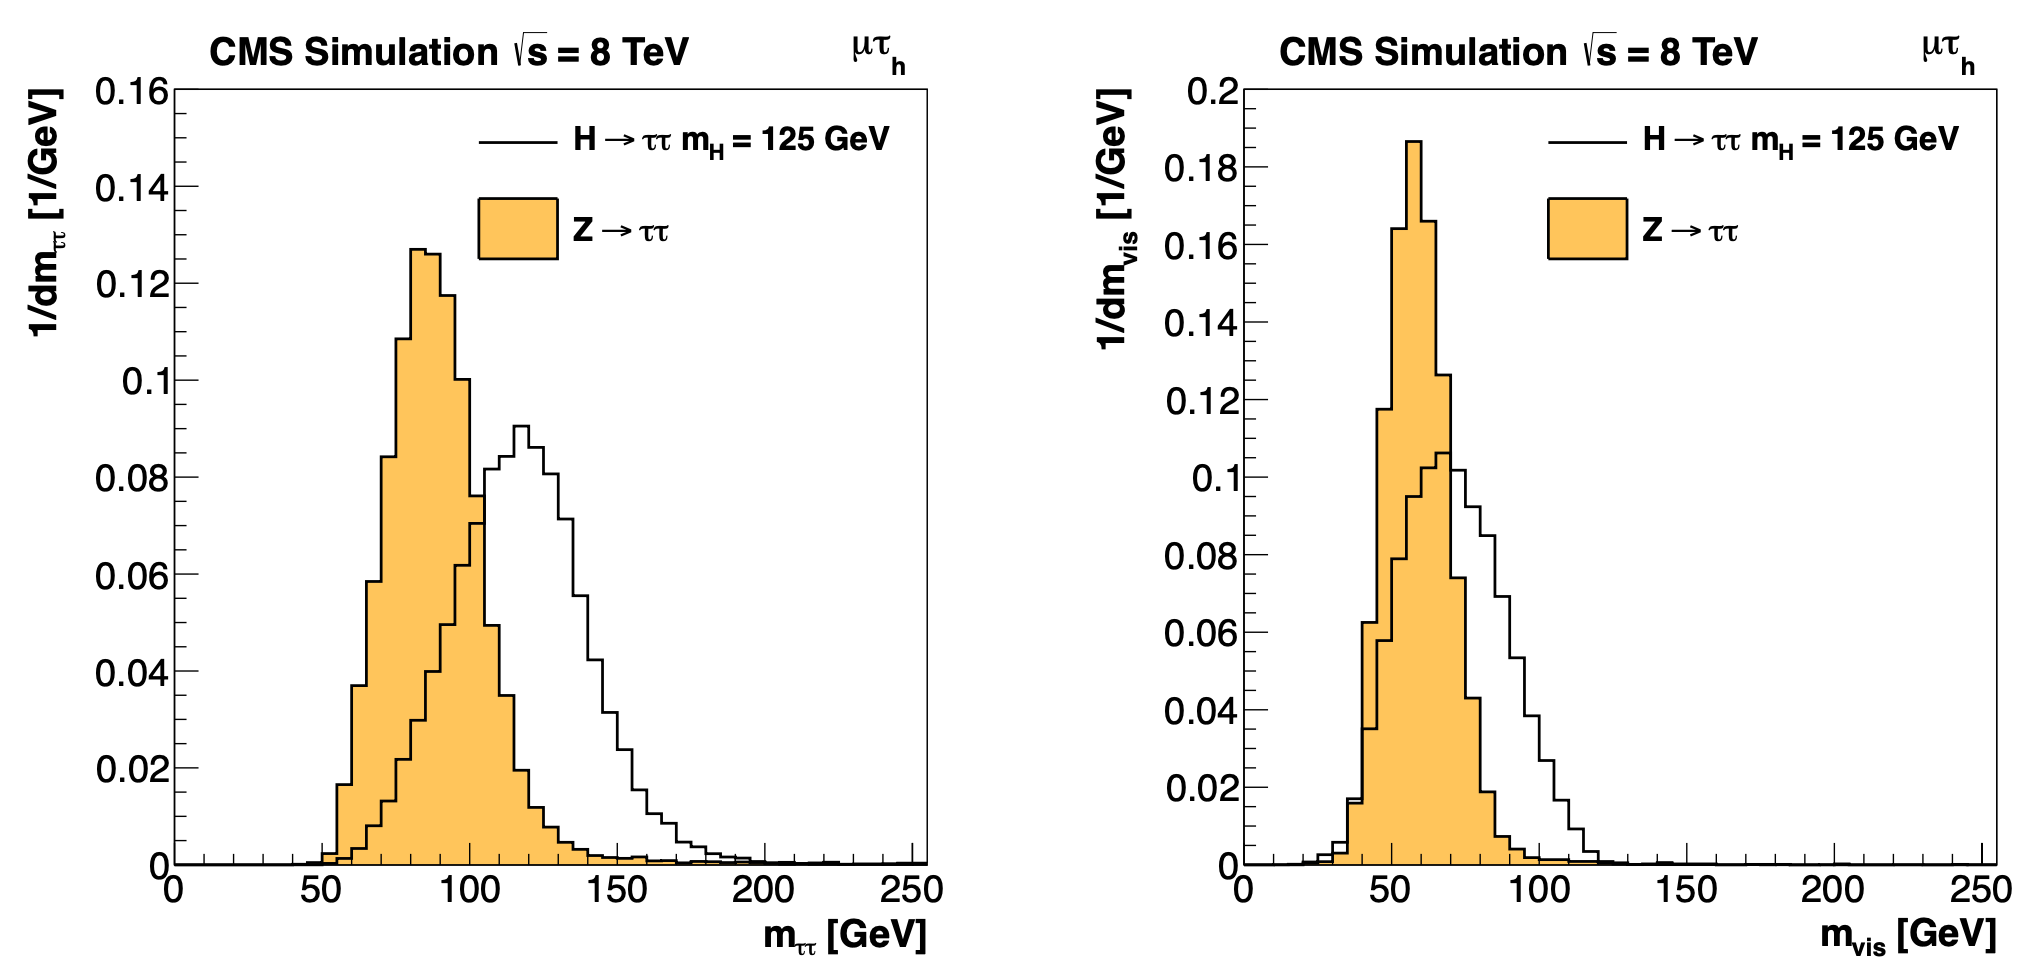
\includegraphics[width=15cm]{figures/ch-12-signal-extraction-statistical-fitting/original_SVFit_resolution_2014_SVFit_Bianchini.png}
    \caption[Distributions of $m_{\tau\tau}$ reconstructed by the classic SVFit algorithm, and masses of visible tau decay products (before SVFit).]{Distributions from \cite{2014_SVFit_Bianchini}, of $m_{\tau\tau}$ after reconstruction with the original SVFit algorithm (\textit{left}), and before SVFit with only the visible tau decay products (\textit{right}), for $H \rightarrow \tau\tau$ signal events of mass $m_H = 125$ GeV (\textit{black line}) and the $Z/\gamma^* \rightarrow \tau\tau$ background (\textit{orange, solid}), in the decay channel $\tau\tau \rightarrow \mu\tau_{h}$.} 
    \label{fig:classic_svfit_resolution}
\end{figure}


\section{FastMTT: optimized SVFit}
FastMTT \cite{CMS-AN-19-032-FastMTT} is a further simplification to the matrix element method of Classic SVFit which has comparable performance but is about 100 times faster. FastMTT drops the matrix element component of the computation without significant impact on the final mass resolution, and simplifies the computation of the transfer functions. The opening angle of the $\tau$ decay products with respect to the initial $\tau$ momenta approaches 0 for $\tau$ with high $\gamma = E_{\tau}/m_{\tau}$, with typical $\tau$ decays from the Z boson decays already satisfying this condition. In this collinear approximation, the dimensionality of the transfer function can be reduced in the computation of FastMTT, while still yielding similar results to Classic SVFit \cite{CMS-AN-19-032-FastMTT}. 



\chapter{Systematic uncertainties}
\label{chapter:ch-12:systematic-uncertainties}
The handling of systematic uncertainties is separated into normalization uncertainties (those that affect the total yield of a variables' distribution) and shape uncertainties (those that shift the distribution of events). Normalization uncertainties are expressed as multiplicative factors, while shape uncertainties are represented as up and down shifts of a variable's distribution.

Up/down shifts of shape uncertainties can change the number of background events in a distribution. For instance, hadronic taus receive corrections from the nominal tau energy scale, with the nominal, up, and down energy scales provided centrally by CMS. For the $\mu\tau_{h}$ channel, an event could have a $\tau_{h}$ with $p_{T}$ just below the offline threshold of 20 GeV (for instance, 19.5 GeV), so in the nominal distribution of $m_{\tau\tau}$ (or any other variable for this channel), the event is excluded. However, when we build our distributions with the tau energy scale ``up" shift, the energy of this $\tau_{h}$ may be scaled up to, say, 20.5 GeV, and now the event passes the offline $p_{T}$ threshold for the single muon trigger, leading to the event's inclusion in the distributions made with the tau energy scale ``up'' shift.

In evaluating the up and down shifts of a specific source of uncertainty, all other corrections and scale factors are held at their nominal values, and the full chain of object and event selection and event categorization is performed to obtain the observable distributions. Any ``downstream" variables that depend on the shifted variable, e.g. the invariant di-tau mass $m_{\tau\tau}$, must be computed for the nominal case, and then re-computed separately for each up and down shift of the tau legs' energy scale.  The objective of this process is to quantify the effect of a single source of uncertainty on the resulting observable distributions. 


\section{Uncertainties associated with physics objects}
Each scale factor and correction described in Ch. \ref{chapter:ch-8:scale-factors-and-corrections} has an associated uncertainty. The binning of the uncertainties follows that of the nominal scale factor value.

\subsection{Uncertainties in the lepton energy scales}
The uncertainties in the tau energy scales \cite{twiki_TAU_POG_tauidrecommendationforrun2} are binned by the tau decay mode and are taken as shape uncertainties treated as uncorrelated across the tau decay modes and years. Same as with the application of the nominal scale factor, when applying the up or down shifts, the missing transverse energy ($p_{T}^{\text{miss}}$) of the event is adjusted so that the 4-vector sum of the tau $p_{T}^{\text{miss}}$ is unchanged.

The uncertainties in the muon energy scale \cite{twiki_MUON_POG_recommendation} are 0.4\% for $|\eta| < 1.2$, 0.9\% for $1.2 < |\eta| < 2.1$, and 2.7\% for $2.1 < |\eta| < 2.4$, and are treated as shape uncertainties, fully uncorrelated between embedded and MC samples.

The uncertainties in the electron energy scale \cite{twiki_Electron_POG_recommendation} in MC are binned in the electron $|\eta|$ and $p_{T}$, and are shown in Fig. \ref{fig:egamma-POG-UL-egamma-scale-factors}. The uncertainties range from 0.5\% to 2.2\% in the barrel, and 0.3\% to 4.1\% in the endcap, across the $p_{T}$ range. The uncertainties for the embedded sample are binned only in $|\eta|$ and are on the order of 0.5\% and 1.25\% for the barrel and endcap \cite{twiki_embedded_preUL_2018}.

There are also uncertainties in the energy scales for electrons and muons misidentified as $\tau_{h}$. The uncertainty for muons misidentified as $\tau_{h}$ is 1\% \cite{twiki_TAU_POG_tauidrecommendationforrun2}. For electrons misidentified as $\tau_{h}$, the uncertainty is binned in barrel/endcap $\eta$ and by 1-prong and 1-prong + $\pi_0$ decays. The probability for $e/\mu$ faking a 3-prong decay mode is much lower. 

\subsection{Uncertainties from other lepton corrections}
Uncertainties associated with the $\tau_{h}$ identification efficiencies are treated as shapes, uncorrelated across the seven $p_{T}$ bins and years. The shape uncertainties in the embedded samples are taken as 50\% correlated with those of the MC samples.

The uncertainties on electron and muon identification efficiencies are taken as normalization uncertainties of 2\% each, with a 50\% correlation between embedded and MC samples.

In the $e\tau_{h}$ channel, there is an additional uncertainty for the vs. jet discrimination efficiency \cite{twiki_TAU_POG_tauidrecommendationforrun2}, because the analysis uses a looser anti-lepton working point (VLoose WP) than the working points used in the measurement of the efficiency (namely, VLoose WP vs e, and Tight WP vs mu). For nominal $\tau_{h}$ $p_{T} < 100$ GeV, an additional uncertainty of 3\% (5\%) is used in MC (embedded), and for high $p_{T}$ an uncertainty of 15\% is used for both.

The uncertainties in trigger efficiencies are taken as shapes \cite{twiki_TAU_POG_tauidrecommendationforrun2}. In the $e\tau_{h}$ and $\mu\tau_{h}$ channels, there are uncertainties for the single and cross lepton triggers, and in the $e\mu$ channel there is one uncertainty each for the two $e+\mu$ triggers, and one combined uncertainty since their trigger phase spaces are not mutually exclusive.

\subsection{Uncertainties from jet energy scale and resolution}
\label{subsec:JEC_sys}
The jet energy scale uncertainties are taken as shape uncertainties: there are eleven in total, with seven correlated across years (labeled ``Year" below) and the remainder uncorrelated across years. They affect the b-tag jet $p_{T}$ and mass, and hence the missing transverse energy $p_{T}^{\text{miss}}$. The shifts are propagated through the b-tagging scale factor calculation and b-tag jet counting. 

The uncertainties in the jet energy correction and resolution \cite{CMS-JME-13-004} \cite{twiki_JetEnergyScale_Uncertainty_Sources_JERC} are as follows:
    \begin{itemize}
        \item \textit{Absolute, AbsoluteYear}: flat absolute scale uncertainties.
        \item \textit{BBEC1, BBEC1Year}: for sub-detector regions, with barrel ``BB" in $|\eta| < 1.3$ and endcap region 1 ``EC1'': $1.3 < |\eta| < 2.5$.
        \item \textit{EC2, EC2 year}: for sub-detector regions, with endcap region 2 ``EC2'' in $2.5 < |\eta| < 3.0$.
        \item \textit{HF, HF year}: for sub-detector regions, with hadron forward ``HF'' in $|\eta| > 3$.
        \item \textit{FlavorQCD}: for uncertainty in jet flavour (uds/c/b-quark and gluon) estimates based on comparing Pythia and Herwig (different MC generator) predictions. 
        \item \textit{RelativeBal}: account for difference between log-linear fits of the two methods used to study the jet energy response: MPF (missing transverse momentum projection fraction) and $p_{T}$ balance.
        \item \textit{RelativeSample}: account for $\eta$-dependent uncertainty due to a difference between relative residuals, observed with dijet and Z+jets in Run D of 2018 data.
        \item \textit{JetResolution}: uncertainty in the jet energy resolution.
    \end{itemize}

\subsection{Uncertainties from b-tagging scale factors}
The b-tagging scale factor has its own set of associated uncertainties (not to be confused with shifts in the b-tagging scale factor due to the propagation of the jet energy scale uncertainties described in the previous section \ref{subsec:JEC_sys}). They are:
\begin{itemize}
    \item \textit{hf}: contamination from heavy flavour (b+c) jets in the light flavour region.
    \item \textit{hfstats1, hfstats2}: linear and quadratic statistical fluctuations from b jets. 
    \item \textit{lf}: contamination from light flavour (udsg+c jets) in the heavy flavour region.
    \item \textit{lfstats1, lfstats2}: linear and quadratic statistical fluctuations from udsg jets.
    \item \textit{cferr, cferr2}: uncertainty for charm jets.
\end{itemize}
The variations for ``lf, hf, hfstats1/2, lfstats1/2'' are applied to both b and udsg jets. For c-flavour jets, only ``cferr1/2'' is applied.

\subsection{Uncertainties from MET}
Samples where recoil corrections were applied (Z+jets, W+jets, and Standard Model Higgs, as described in Section \ref{chapter:ch-8:scale-factors-and-corrections}) have uncertainties from the response and resolution of the hadronic recoil against the leptonic system. These are each binned in jet multiplicity.

\section{Uncertainties associated with samples used}
Normalization uncertainties related to the samples used are:
\begin{itemize}
    \item \textit{Cross-section uncertainties}: $\sigma(t\bar{t})$: 4.2\%, $\sigma$(diboson): 5\%,  $\sigma$(single top): 5\%, $\sigma$(ggH): 3.2\%, $\sigma$(qqH): 2.1\%, $\sigma$(WH): 1.9\%, $\sigma$(ZH): 1.3\%, $\sigma$(ttH): 3.6\%
    \item \textit{Uncertainties in QCD renormalization scale}: QCD scale(qqH): +0.43\%-0.33\%, QCD scale(WH): +0.5\%-0.7\%, QCD scale(ttH): +5.8\%-9.2\%
    \item \textit{Branching ratio uncertainties}: BR(H$\rightarrow\tau\tau$): 1.8\%, and BR(H$\rightarrow$WW): 1.5\%.
    \item \textit{Normalization uncertainties}: 2\% for Drell-Yan, 4\$ for embedded, 20\% pre-fit for the QCD multijet background in the $e\mu$ channel, 20\% pre-fit for the jet faking background.
\end{itemize}

The $t\bar{t}$ process has additional acceptance uncertainties from QCD scale variation and parton shower uncertainties \cite{twiki_Top_systematics}.  Parton shower uncertainties originate from the modeling of perturbative and non-perturbative QCD effects handled in parton shower MC generators. The scale variations are determined from the envelope of the 6 provided shapes due to variations in the factorization scale, renormalization scale, and their combined variation \cite{twiki_Top_systematics}.

The Z $p_{T}$ reweighing uncertainty in Drell-Yan samples is taken to be 10\% of the nominal value, taken as a shape uncertainty. 

The fake rate uncertainties are taken as shape uncertainties. For the weight applied to scale up anti-isolated events in cross-trigger regions, 20\% of the nominal weight is taken as a shape uncertainty.

\section{Other uncertainties}
A 3.6\% yield uncertainty in the signal is used to cover uncertainties in the parton distribution functions, $\alpha_s$ (fine structure constant), and QCD scale. 

Normalization uncertainties from luminosity are applied to all MC samples, divided into those uncorrelated across years, those correlated between 2017 and 2018, and one for 2018 \cite{twiki_LUMI_POG_recommendation}.

\section{Pulls and impacts}
The top impacts and pulls computed for the combination of all channels and years is shown in Fig. \ref{fig:impacts_pages_1_2}. The top impacts are related to uncertainty in the signal sample and cross-section of the $t\bar{t}$ cross-section, and also the yields of the jet faking $\tau_{h}$ background, which is a major background in all channels and expected to be constrained due to the yield uncertainty which is taken to be 20\% pre-fit. 

\begin{figure}[ht]
    \begin{center}
        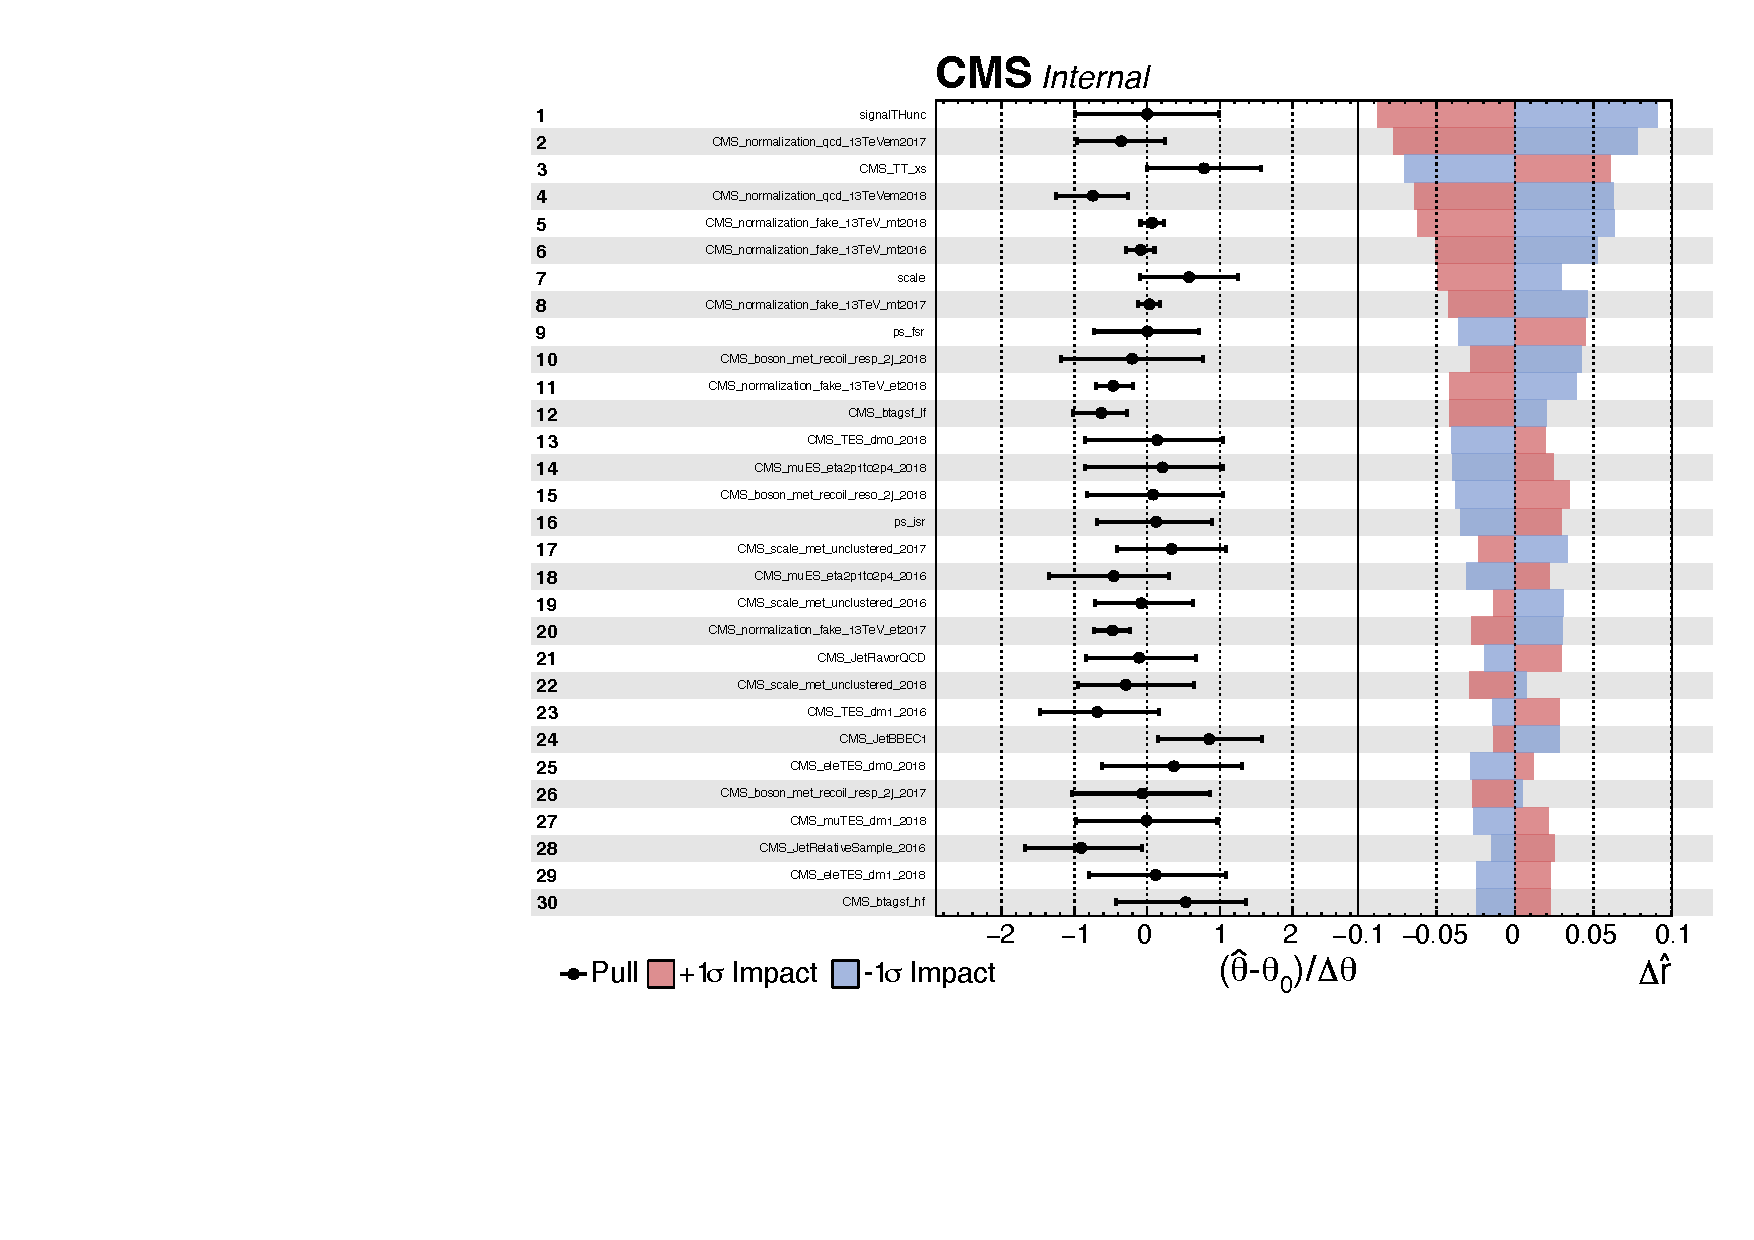
\includegraphics[width=0.8\textwidth]{figures/ch-11-systematic-uncertainties/impacts-all-1.pdf}\\
        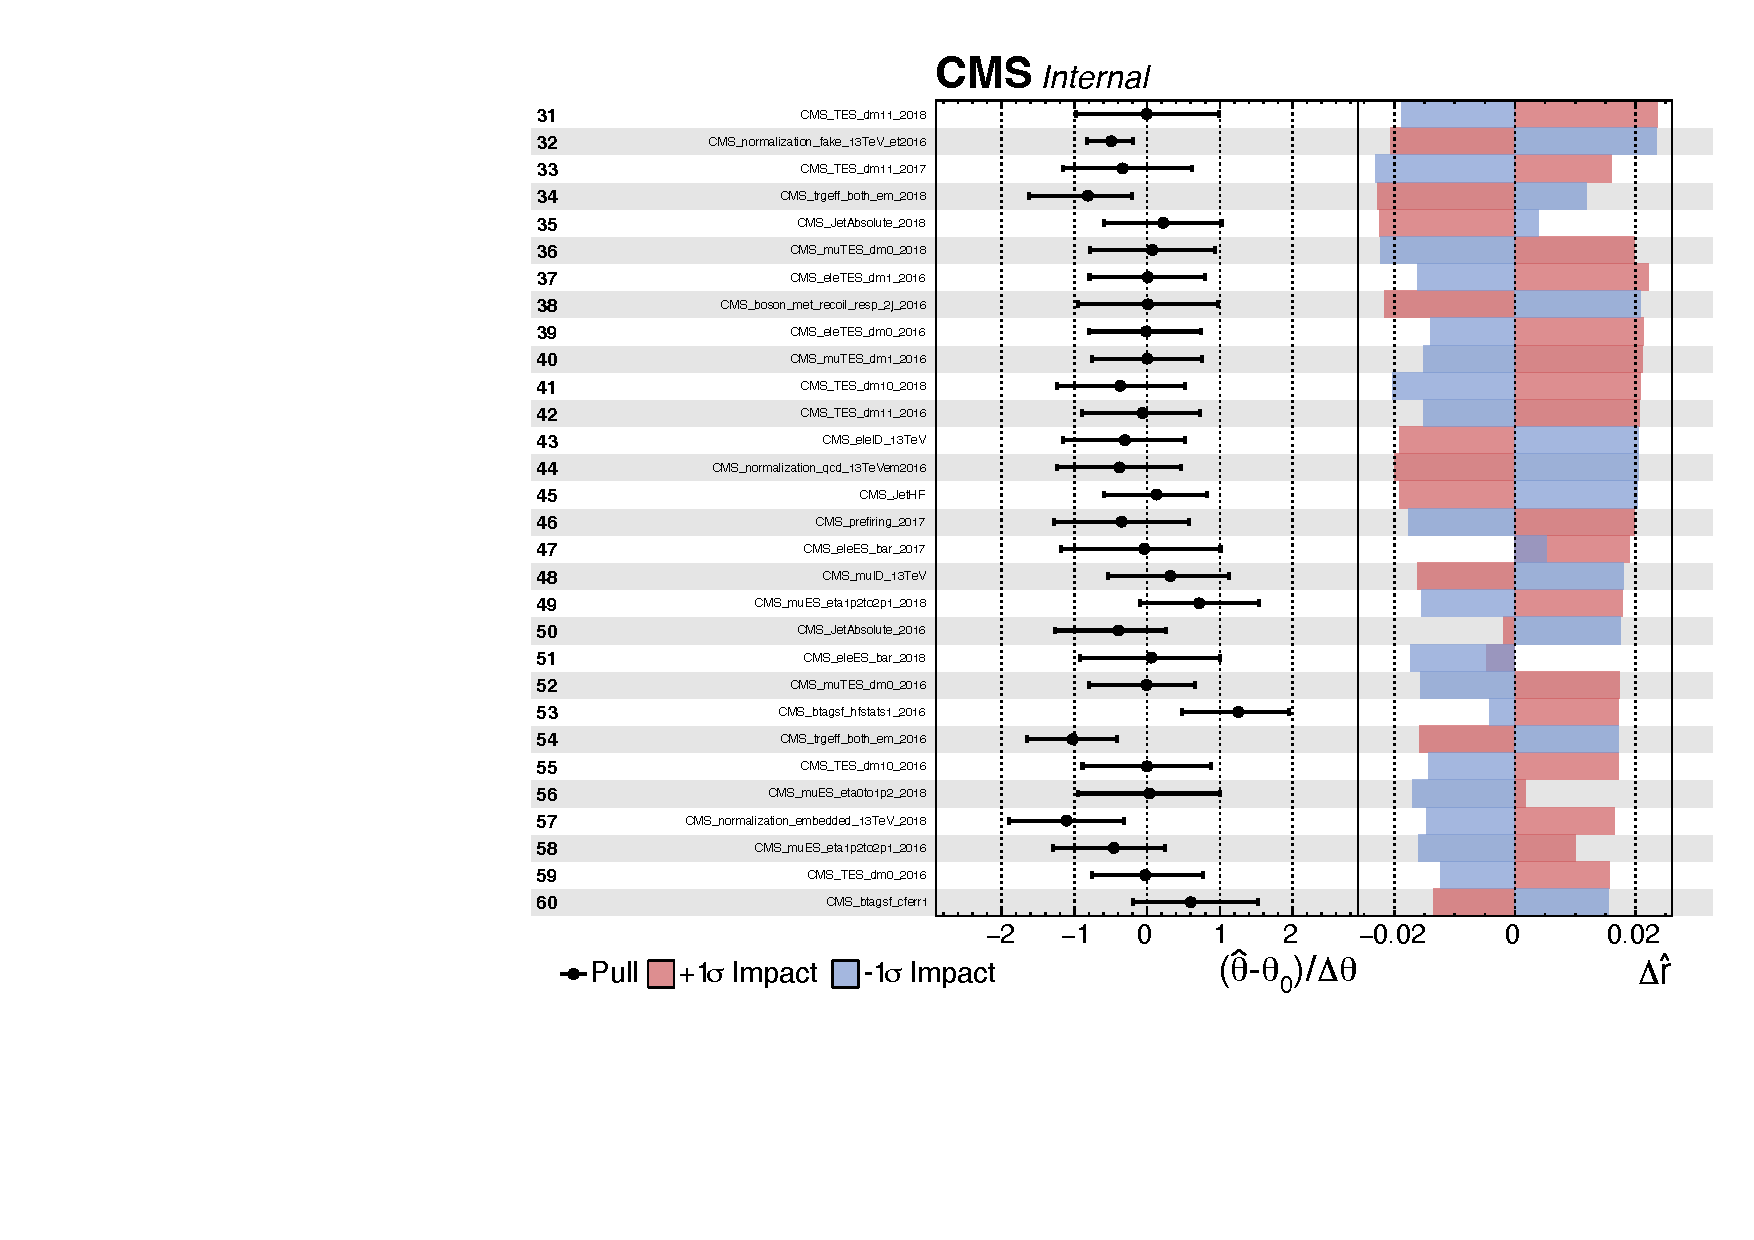
\includegraphics[width=0.8\textwidth]{figures/ch-11-systematic-uncertainties/impacts-all-2.pdf}
    \end{center}
    \caption[Top sixty impacts for the combination of all channels and years.]{Top sixty impacts for the combination of all channels and years \cite{CMS-AN-20-213}.}
    \label{fig:impacts_pages_1_2}
\end{figure}


\chapter{Signal extraction}
\label{chapter:ch-13:signal-extraction}
In this chapter we describe the statistical methodology used to perform signal extraction. 

\section{Model building and parameter estimation}
In the frequentist interpretation of probability, an experiment measuring an observable can be repeated, resulting in different values of the observable, e.g. the invariant mass of a candidate Higgs boson in a search for the Higgs \cite{2011-Statistics-Cranmer}. The ensemble of values of the observable $x$ gives rise to the probability density function (PDF) $f(x)$, which has the important property that it is normalized to unity:
\begin{equation*}
    \int f(x) \, dx = 1 \,.
\end{equation*}
A parametric family of PDFs
\begin{equation*}
    f(x|\alpha) \, ,
\end{equation*}
read ``$f$ of $x$ given $\alpha$", is referred to as a probability model or model. The parameters $\alpha$ typically represent parameters of the theory or an unknown property of the detector's response. The parameters are not frequentist in nature, unlike $x$. Out of all the parameters, typically only a few are of interest, and are called the parameters of interest (POI), labeled $\mu$ here. The remaining are referred to as nuisance parameters (NP) \cite{2011-Statistics-Cranmer} and are labeled $\boldsymbol{\theta}$.

$f(x)$ is the probability density for the observable in one event and we wish to describe the probability density for a dataset with many events, $\mathcal{D} = \{x_1, ..., x_n\}$, called the total probability model $\boldsymbol{f}$. For instance, if we also have a prediction for the total number of events expected, called $\nu$, we also account for the overall Poisson probability for observing $n$ events given $\nu$ expected:
\begin{equation}
    \boldsymbol{f}(\mathcal{D}|\nu, \alpha) = \text{Poisson}(n|\nu) \prod_{e=1}^{n} f(x_e | \alpha)
\end{equation}

The likelihood function $L(\alpha)$ is numerically equivalent to $f(x|\alpha)$ for fixed $x$, or $\boldsymbol{f}(\mathcal{D}|\alpha)$ with $\mathcal{D}$ fixed \cite{2011-Statistics-Cranmer}. The likelihood function is not a probability density for $\alpha$ and is not normalized to unity:
\begin{equation*}
    \int L(\alpha) \, d(\alpha) \neq 1 \, .
\end{equation*}
i.e. the likelihood function is the value of $f$ as a function of $\alpha$ given a fixed value of $x$.

To estimate the parameter $\alpha$ we use an estimator, which is a function of the data. Take for example the measurement of data distributed according to a Gaussian probability density $f(x| \mu,\sigma) = \text{Gauss}(x|\mu,\sigma)$. One possible estimator of the mean $\mu$, is the mean of the measured data points $\bar{x} = \sum_{i = 1}^{n} x_i / n$ \cite{2011-Statistics-Cranmer}. 

A commonly used estimator in physics is the maximum likelihood estimator (MLE), defined as the value $\alpha$ which maximizes the likelihood function $L(\alpha)$. This value, labeled $\hat{\alpha}$, also maximizes $\ln L(\alpha)$ and minimizes $-\ln L(\alpha)$. By convention the $-\ln L(\alpha)$ is minimized, in a process called ``fitting", and the maximum likelihood estimate is called the ``best fit value". 


% Profile likelihood ratios

% How to get a Confidence Level 

% Asimov dataset

\section{Hypothesis testing}
In this section we next introduce concepts related to hypothesis testing such as the test statistic constructed from the ratio of likelihood functions.

The objective of a likelihood analysis is to distinguish different models representing the various hypotheses, and determine the one that best explains the experimental outcome. In a search for new physics, a signal is additive on top of the background. The background-only hypothesis is the null hypothesis, and the signal-plus-background hypothesis is the alternative. 

As a simple example, take the $p$-value test, for an experiment where we count events in the signal region, $n_{SR}$, and expect $\nu_B$ background events and $\nu_S$ events from the signal \cite{2011-Statistics-Cranmer}. Then 
\begin{enumerate}
    \item The null hypothesis ($H_0$), i.e. the background-only hypothesis in this experiment, with the probability modeled by Poisson($n_{SR}|\nu_B$).
    \item The alternate hypothesis ($H_1$), i.e. signal-plus-background hypothesis, with the probability modeled by Poisson($n_{SR}|(\nu_B + \nu_S)$).
\end{enumerate}
The compatability of the observed data $\nu^0_{SR}$ and the null hypothesis, is quantified as the probability that the background-only hypothesis would produce at least as many events as was observed. This probability is the $p$-value: 
\begin{equation}
    p = \sum_{n = n^0_{SR}}^{\infty} \text{Poisson}(n | \nu_B) \, .
\end{equation}
If the $p$-value is very small, we might reject the null hypothesis. The $p$-value is not the probability of the null hypothesis given the data; rather, it expresses the probability that data with a certain property was obtained, assuming the null hypothesis \cite{2011-Statistics-Cranmer}.

The $p$-value is an example of a test statistic $T$, which maps the data to a single real number. The Neyman-Pearson lemma states that out of the infinite possibilities of choices of test statistic, the uniformly most powerful test statistic is the likelihood ratio $T_{NP}$ \cite{2011-Statistics-Cranmer}:

\begin{equation}
    T_{NP}(\mathcal{D}) = \frac{L(\mathcal{D} | {H_1})}{L(\mathcal{D}|{H_0})}
\end{equation}
To reiterate, the test statistic $T$ is a real-valued function of the data, implying that a particular probability model $\boldsymbol{f}(\mathcal{D}|\boldsymbol{\alpha})$ implies a distribution of the test statistic, $f(T|\boldsymbol{\alpha})$, which depends on the value of $\alpha$. With this distribution in hand, the $p$-value can be evaluated in the followng equivalent formulations:
\begin{align}
    p(\boldsymbol{\alpha}) &= \int_{T_0}^{\infty} f(T|\boldsymbol{\alpha}) \, dT  \\
              &= \int \boldsymbol{f}(\mathcal{D} | \boldsymbol{\alpha}) \, \theta(T(\mathcal{D}) - T_0) \, d\mathcal{D} \\
              &= P(T \geq T_0 | \boldsymbol{\alpha})
\end{align}
where $T_0$ is the value of $T$ based on the observed data, and $\theta()$ is the Heaviside function. The size of the test is conventionally chosen to be 10\%, 5\%, or 1\%. As the $p$-value depends on $\boldsymbol{\alpha}$ (both the POI and NP), the null hypothesis should not be rejected if the $p$-value is larger than the size of the test for any value of the nuisance parameters.

\section{Confidence intervals}
In an example of the measurement of the Standard Model Higgs boson, $\boldsymbol{\alpha}_{\text{POI}} = (\sigma/ \sigma_{SM}, M_H)$, with $\sigma/\sigma_{SM}$ is the ratio of the production cross-section for Higgs with respect to its value in the SM, and $M_H$ is the unknown mass of the Higgs, values of these parameters outside specific bounds are said to be ``excluded at the 95\% confidence level''. These allowed regions are called confidence levels or confidence regions, and the parameter values outside of them are considered excluded \cite{2011-Statistics-Cranmer}. A 95\% confidence interval does not mean that there is a 95\% chance that the true value of the parameter is inside the interval. Rather, a 95\% confidence interval covers the true value 95\% of the time (even though we do not know the true value). 

To construct a confidence interval for a parameter $\alpha$, the Neyman Construction is used to invert a series of hypothesis tests; i.e. for each possible value of $\alpha$, the null hypothesis is treated as $\alpha$, and we perform a hypothesis test based on a test statistic. To construct a 95\% confidence interval, we construct a series of hypothesis tests with size of 5\%. The confidence interval $I(\mathcal{D})$ is constructed by taking the set of parameter values $\boldsymbol{\alpha}$ where the null hypothesis is accepted:
\begin{equation}
    I(\mathcal{D}) = \{ \boldsymbol{\alpha} | P(T(\mathcal{D}) > k_\alpha | \boldsymbol{\alpha}) < \alpha \} \, ,
\end{equation} 
where $T(\mathcal{D})$ is the test statistic, and the last $\alpha$ (not bolded) and the subscript $k_\alpha$ refer to the size of the test. A schematic of the Neyman construction is shown in Fig. \ref{fig:neyman-construction}. In a more generalized case, the $x$-axis is the test statistic $T$.

\begin{figure}[ht]
    \centering
    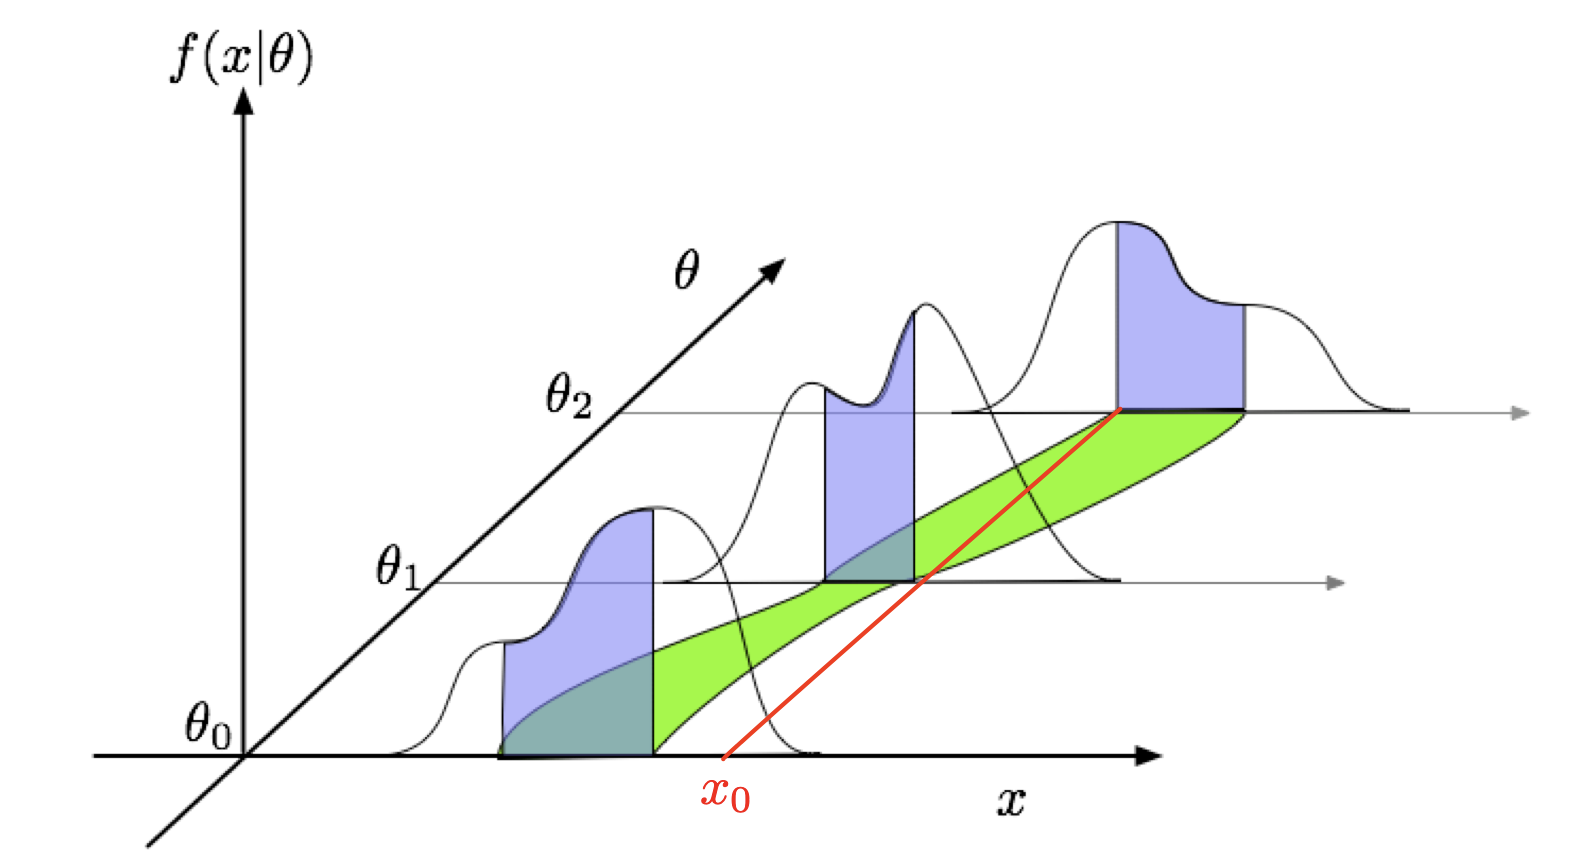
\includegraphics[width=15cm]{figures/ch-13-signal-extraction/schematic_neyman_construction.png}
    \caption[Schematic of the Neyman construction for confidence intervals.]{Schematic of the Neyman construction for confidence intervals \cite{2011-Statistics-Cranmer}. For each value of $\theta$, we find a region in $x$ where $\int f(x|\theta) dx$ satisfies the size of the test (\textit{blue}). These regions form a confidence belt (\textit{green}). The intersection of the observation $x_0$ (\textit{red}) with the confidence belt defines the confidence interval $[\theta_1, \theta_2]$ \cite{2011-Statistics-Cranmer}.} 
    \label{fig:neyman-construction}
\end{figure}

\section{Profiling}

In this section we describe a frequentist statistical procedure based on the profile likelihood ratio test statistic, which is implemented using asymptotic distributions.

With a multi-parameter likelihood function $L(\boldsymbol{\alpha})$, the the maximum likelihood of one specific parameter $\alpha_p$ with other parameters $\boldsymbol{\alpha}_o$ fixed, is called the conditional maximum likelihood estimate and is denoted $\doublehat{\alpha}_p(\boldsymbol{\alpha_0})$.
The process of choosing specific values of the nuisance parameters for a given value of $\mu$, $\mathcal{D}_{\text{simulated}}$, and value of global observables $\mathcal{G}$ is called profiling. From the full list of parameters $\boldsymbol{\alpha}$, we denote the parameter of interest $\mu$, and the nuisance parameters $\boldsymbol{\theta}$.

We construct the profile likelihood ratio,
\begin{equation}
    \lambda(\mu) = \frac{L(\mu, \doublehat{\boldsymbol{\theta}}(\mu))}{L({\mu, \hat{\boldsymbol{\theta}}})}
\end{equation}
which depends explicitly on the parameter of interest $\mu$, implicitly on the data $\mathcal{D}_{\text{sim}}$ and global observables $\mathcal{G}$, and is independent of the nuisance parameters $\boldsymbol{\theta}$, which have been eliminated in profiling \cite{2011-Statistics-Cranmer}.

The main conceptual reason for constructing the test statistic from the profile likelihood ratio is that asymptotically (i.e. for measurements with many events) the distribution of the profile likelihood ratio $\lambda(\mu = \mu_{\text{true}})$ is independent of the values of the nuisance parameters \cite{2011-Statistics-Cranmer}. 

The following $p$-value is used to quantify the consistency with the hypothesis of a signal strength of $\mu$:
\begin{equation}
    p_\mu = \int_{\tilde{q_{\mu, \text{obs}}}}^{\infty} f(\tilde{q}_\mu | \mu, \doublehat{\boldsymbol{\theta}}(\mu, \text{obs})) \, d\tilde{q}_\mu
\end{equation}

% TODO: elaborate (section 3.3 of Cranmer https://cds.cern.ch/record/2004587/files/267-308%20Cranmer.pdf)

\section{Modified frequentist method: $CL_{S}$}
In the

\section{Combining of multiple channels}
Analyses frequently have multiple search channels which need to be combined \cite{2011-Cowan-et-al}. We assume that there is one strength parameter $\mu$ that is the same for all channels. Each channel $i$ has a likelihood function $L_{i} (\mu, \boldsymbol{\theta}_i)$, where $\boldsymbol{\theta_i}$ represents the set of nuisance parameters for the $i$th channel, some of which may be common between the channels. If the channels are statistically independent, the full likelihood function is the product
\begin{equation}
    L(\mu, \boldsymbol{\theta}) = \prod_{i} L_i (\mu, \boldsymbol{\theta_i})
\end{equation}
where $\boldsymbol{\theta}$ is the complete set of all nuisance parameters. The profile likelihood ratio is 
\begin{equation}
    \lambda(\mu) = \frac{ \prod_i L_i(\mu, \hat{\hat{\boldsymbol{\theta}}}_i) }{ \prod_i L_i(\mu, \hat{\boldsymbol{\theta}}_i)}
\end{equation}

% TODO: finish this section once I also define what a profile likelihood ratio is

% ch 13 statistical fitting
\chapter{Results}
\section{Results from $bb\tau\tau$}

The postfit final $m_{\tau\tau}$ distributions in the signal region (SR) and control regions (CRs) for 1 and 2 b-tag jet multiplicities, are shown for the $\mu\tau_{h}$ channel in Fig. \ref{fig:results_mtt_postfit_mtall}, $e\tau_{h}$ channel in Fig. \ref{fig:results_mtt_postfit_etall}, and $e\mu$ channel in Fig. \ref{fig:results_mtt_postfit_emall}.
\begin{figure}[ht]
    \begin{center}
        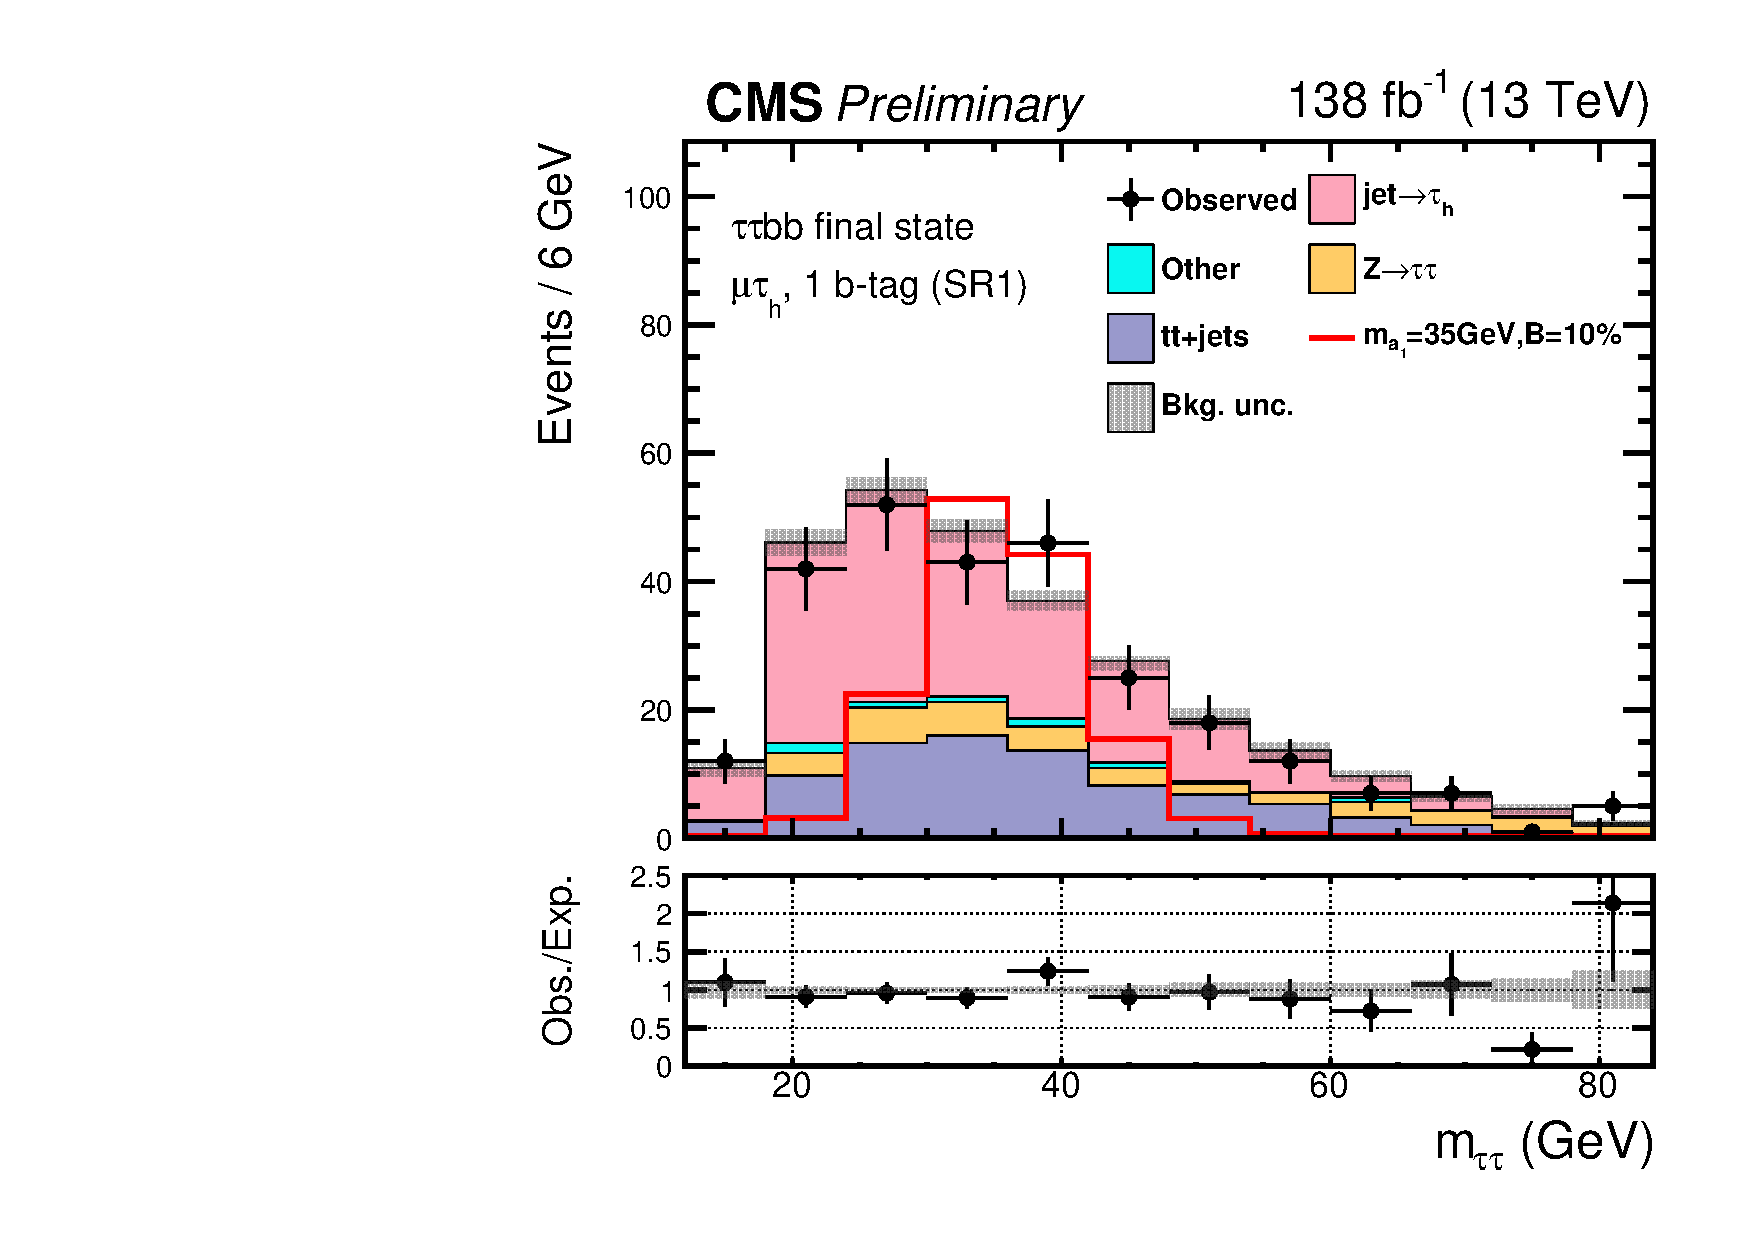
\includegraphics[width=0.32\textwidth]{figures/ch-14-results/mt_all_1_post_prelim-yes.pdf}
        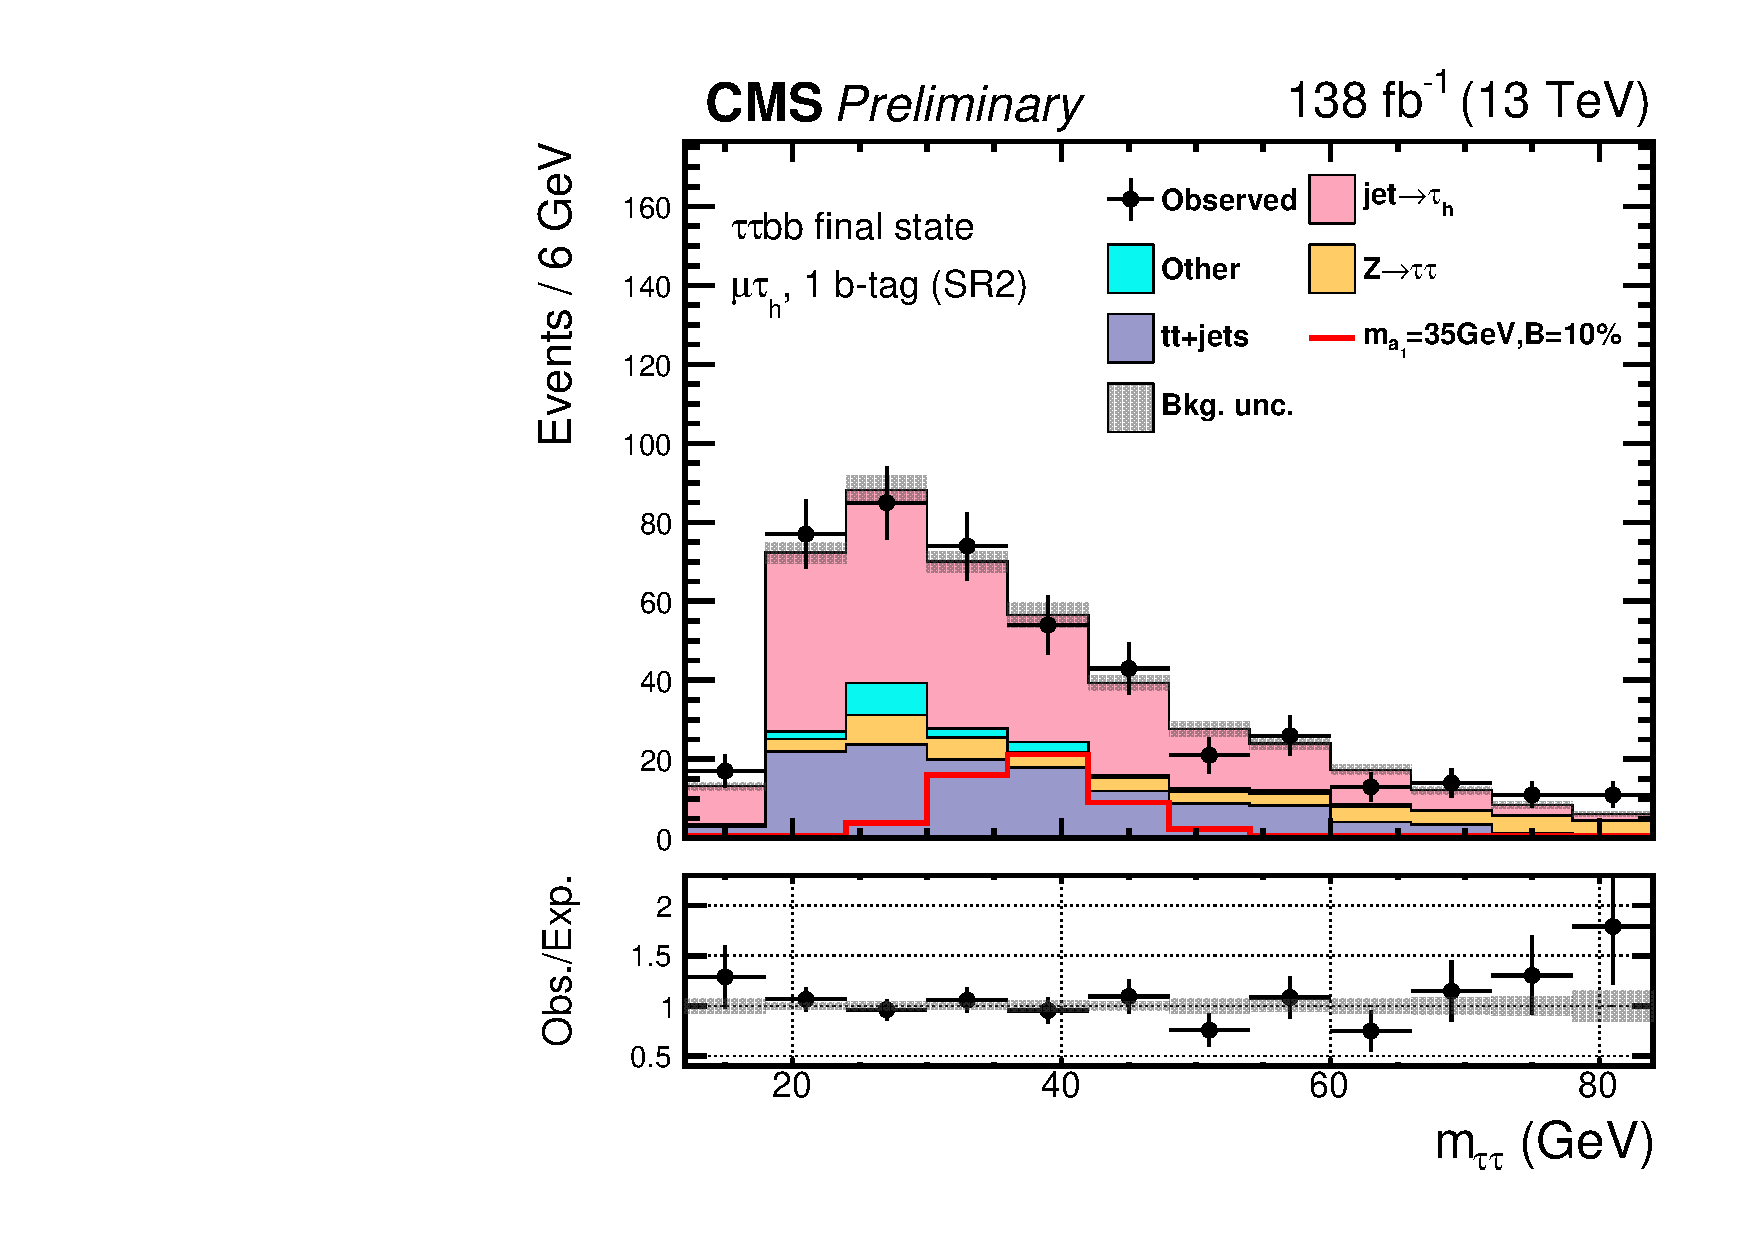
\includegraphics[width=0.32\textwidth]{figures/ch-14-results/mt_all_2_post_prelim-yes.pdf}
        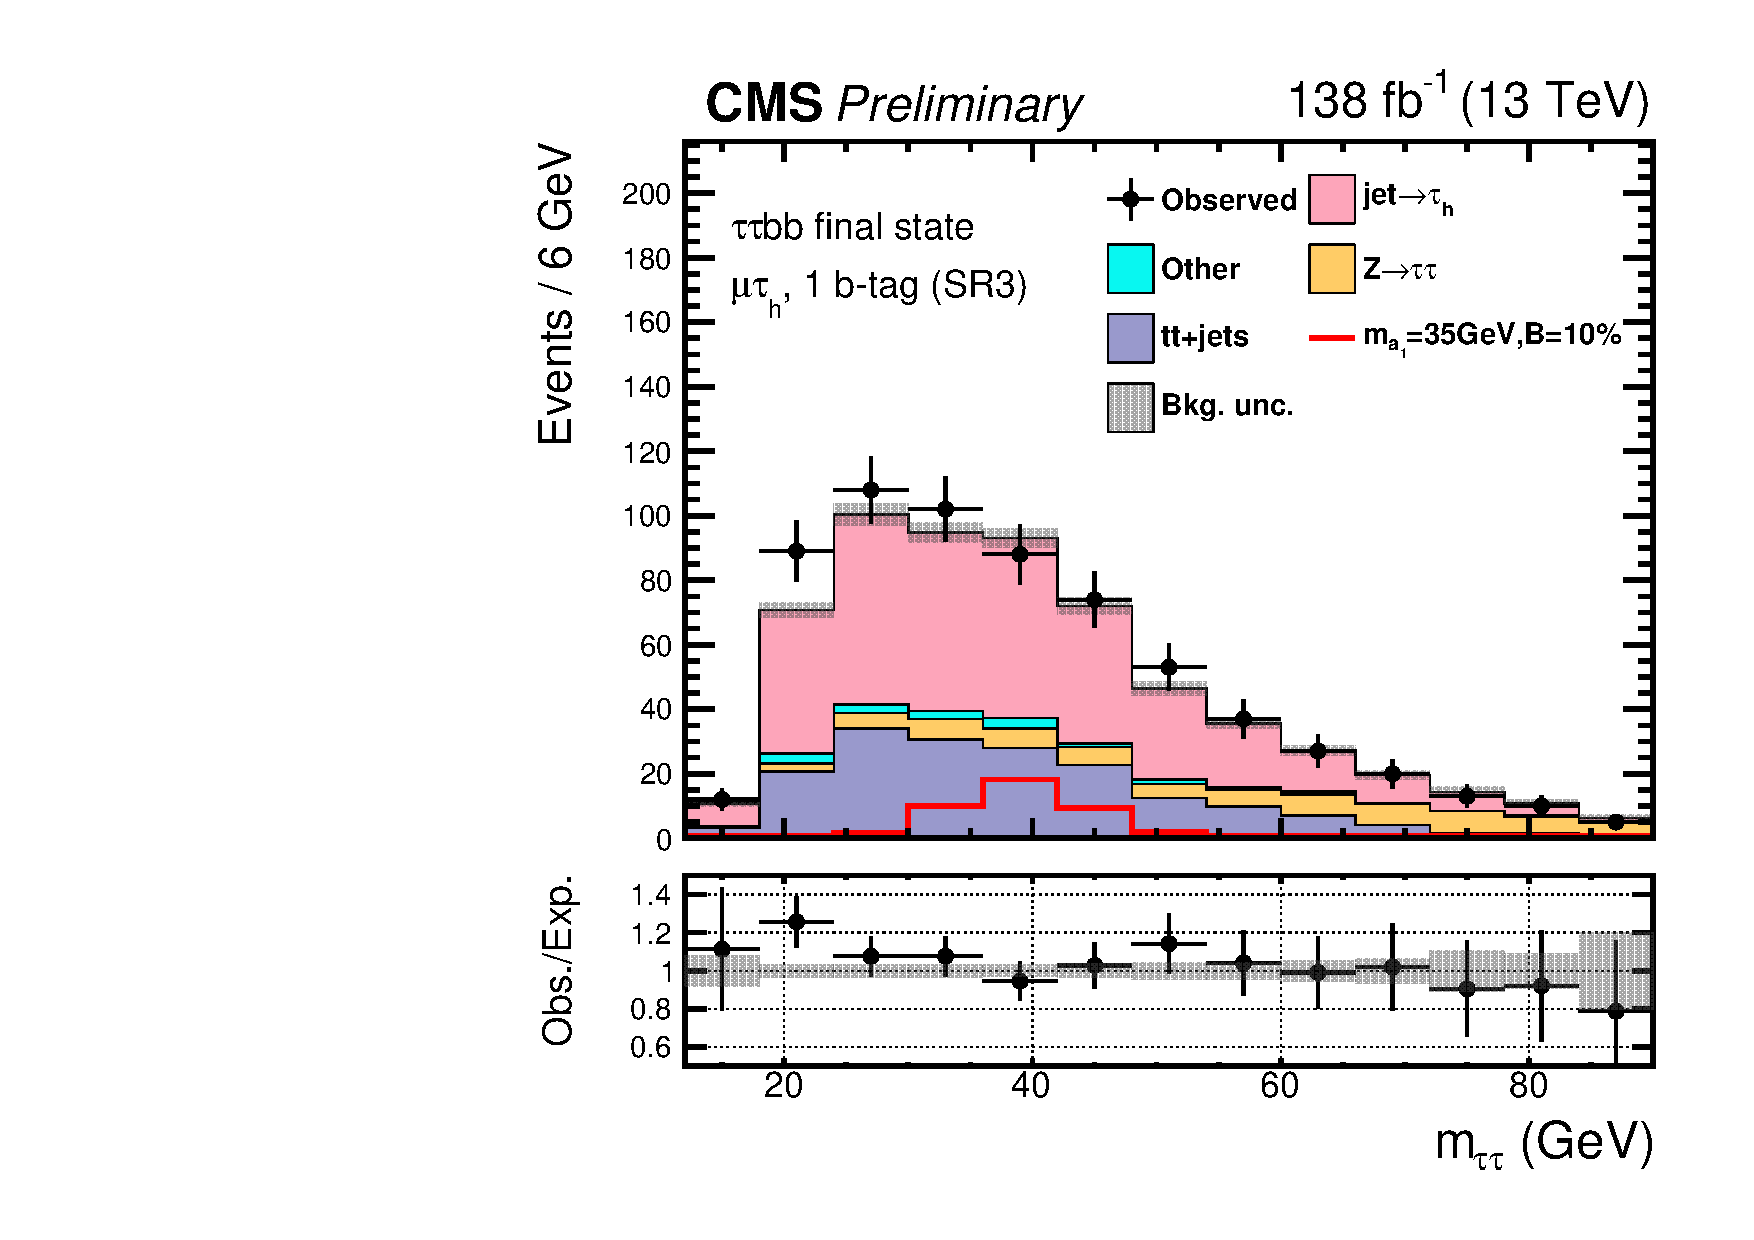
\includegraphics[width=0.32\textwidth]{figures/ch-14-results/mt_all_3_post_prelim-yes.pdf}\\
        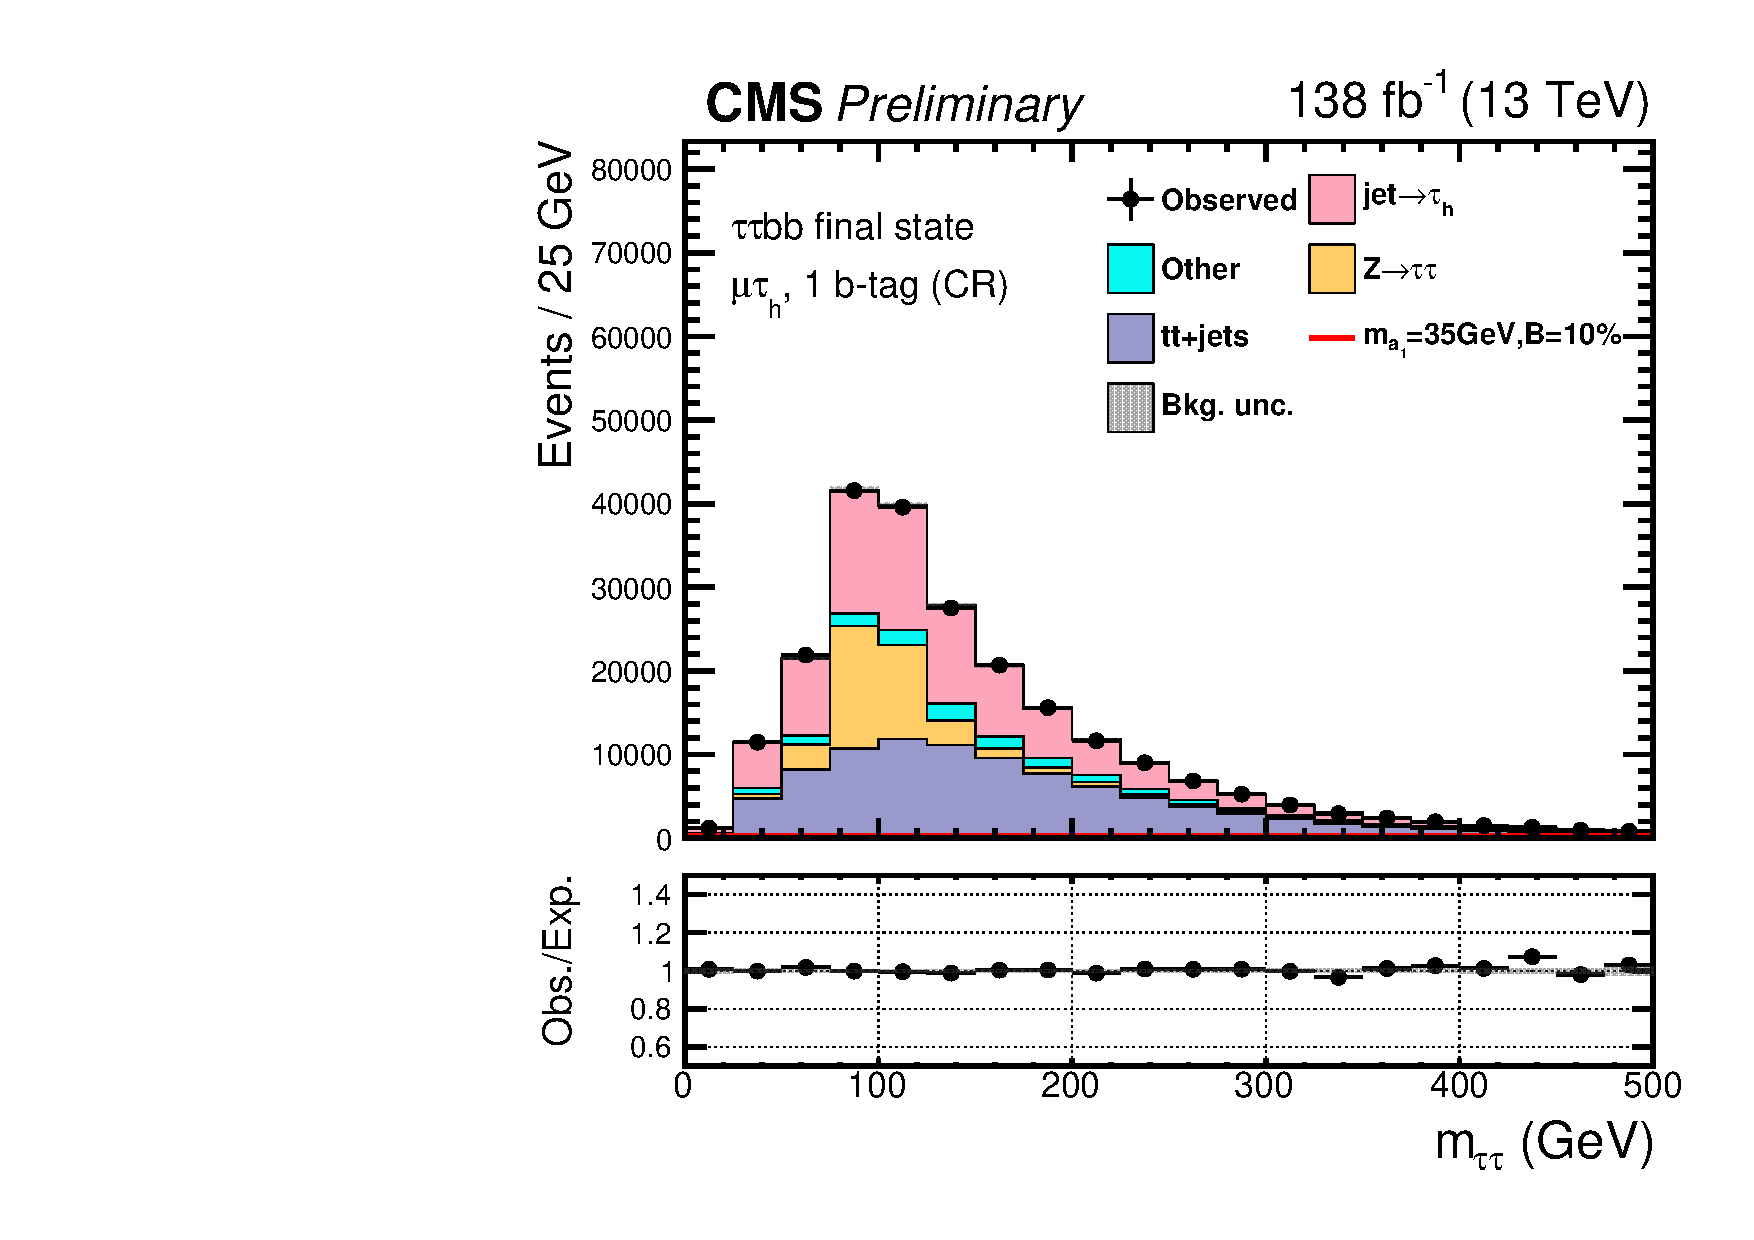
\includegraphics[width=0.32\textwidth]{figures/ch-14-results/mt_all_4_post_prelim-yes.pdf}
        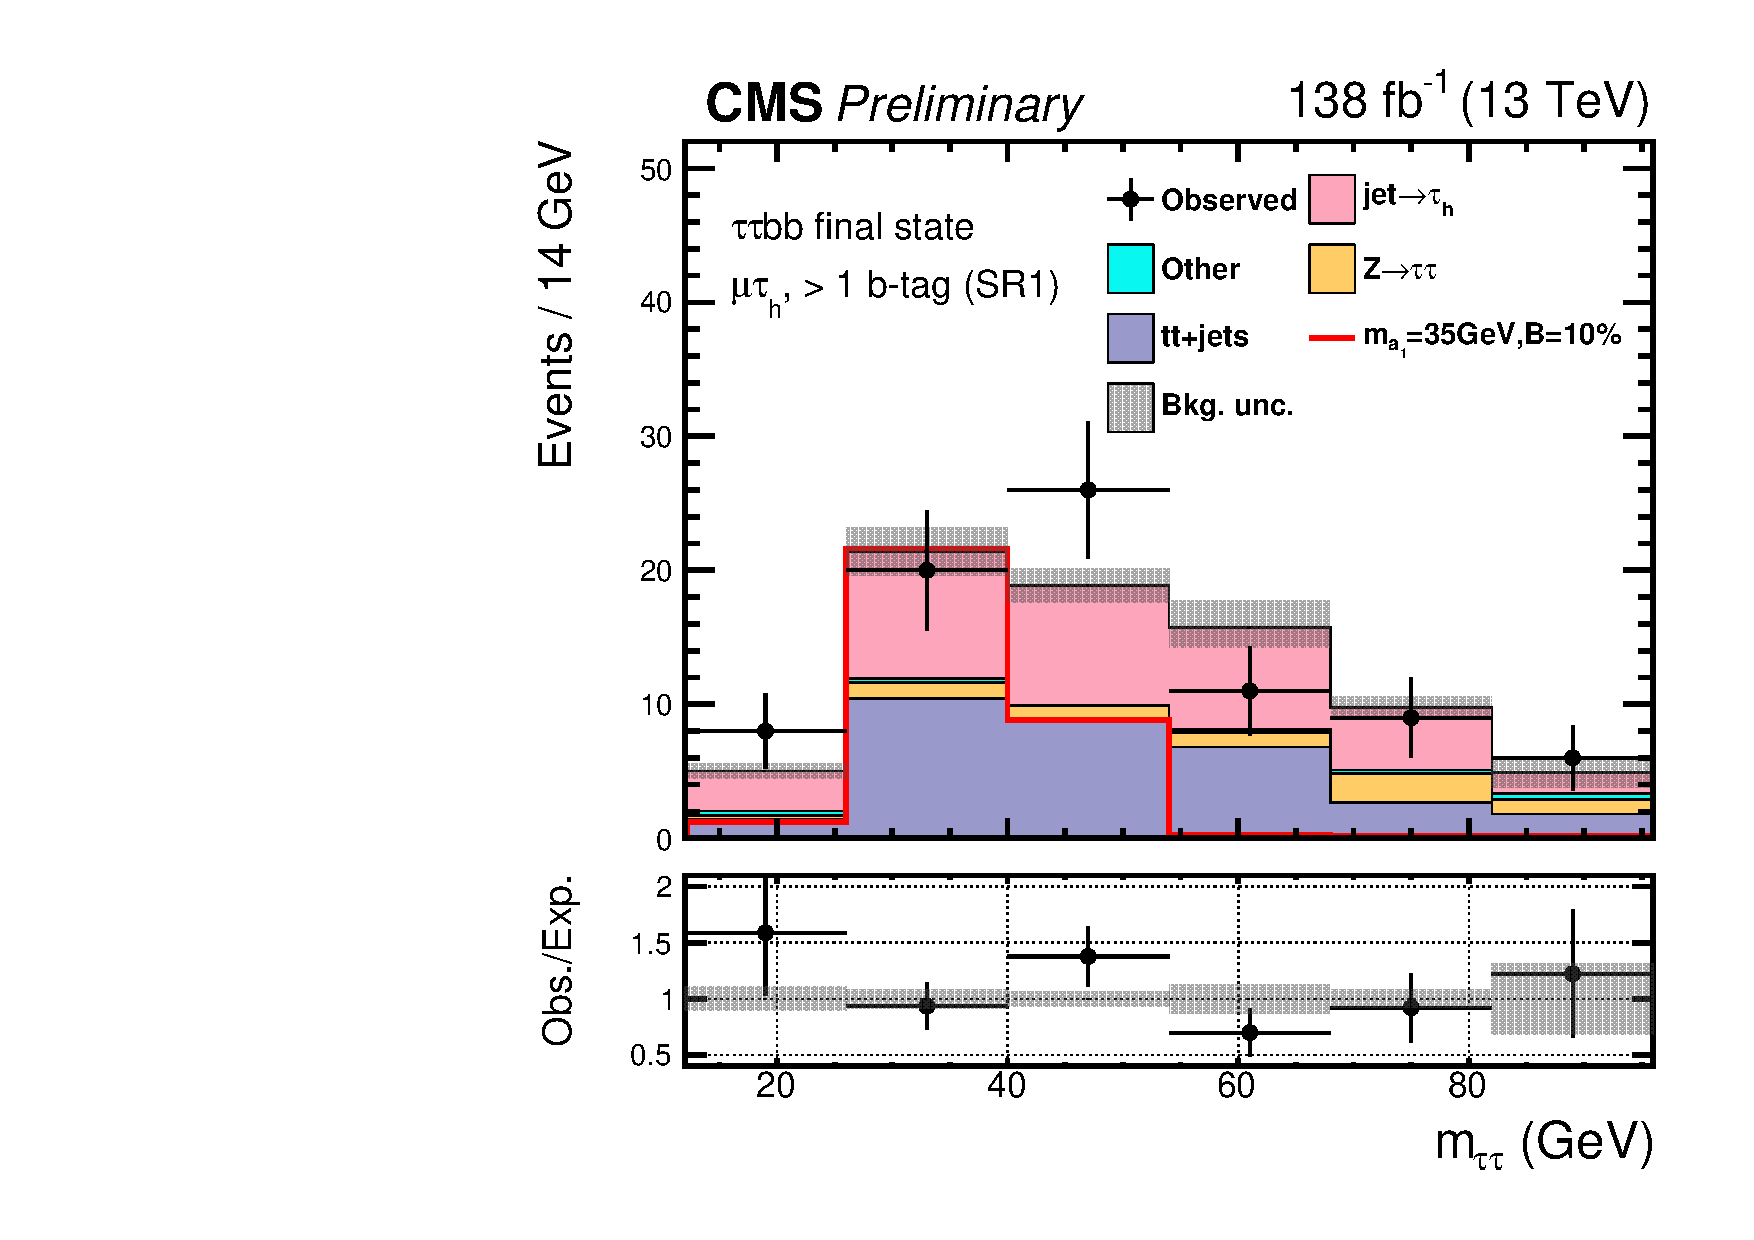
\includegraphics[width=0.32\textwidth]{figures/ch-14-results/mt_all_5_post_prelim-yes.pdf}
        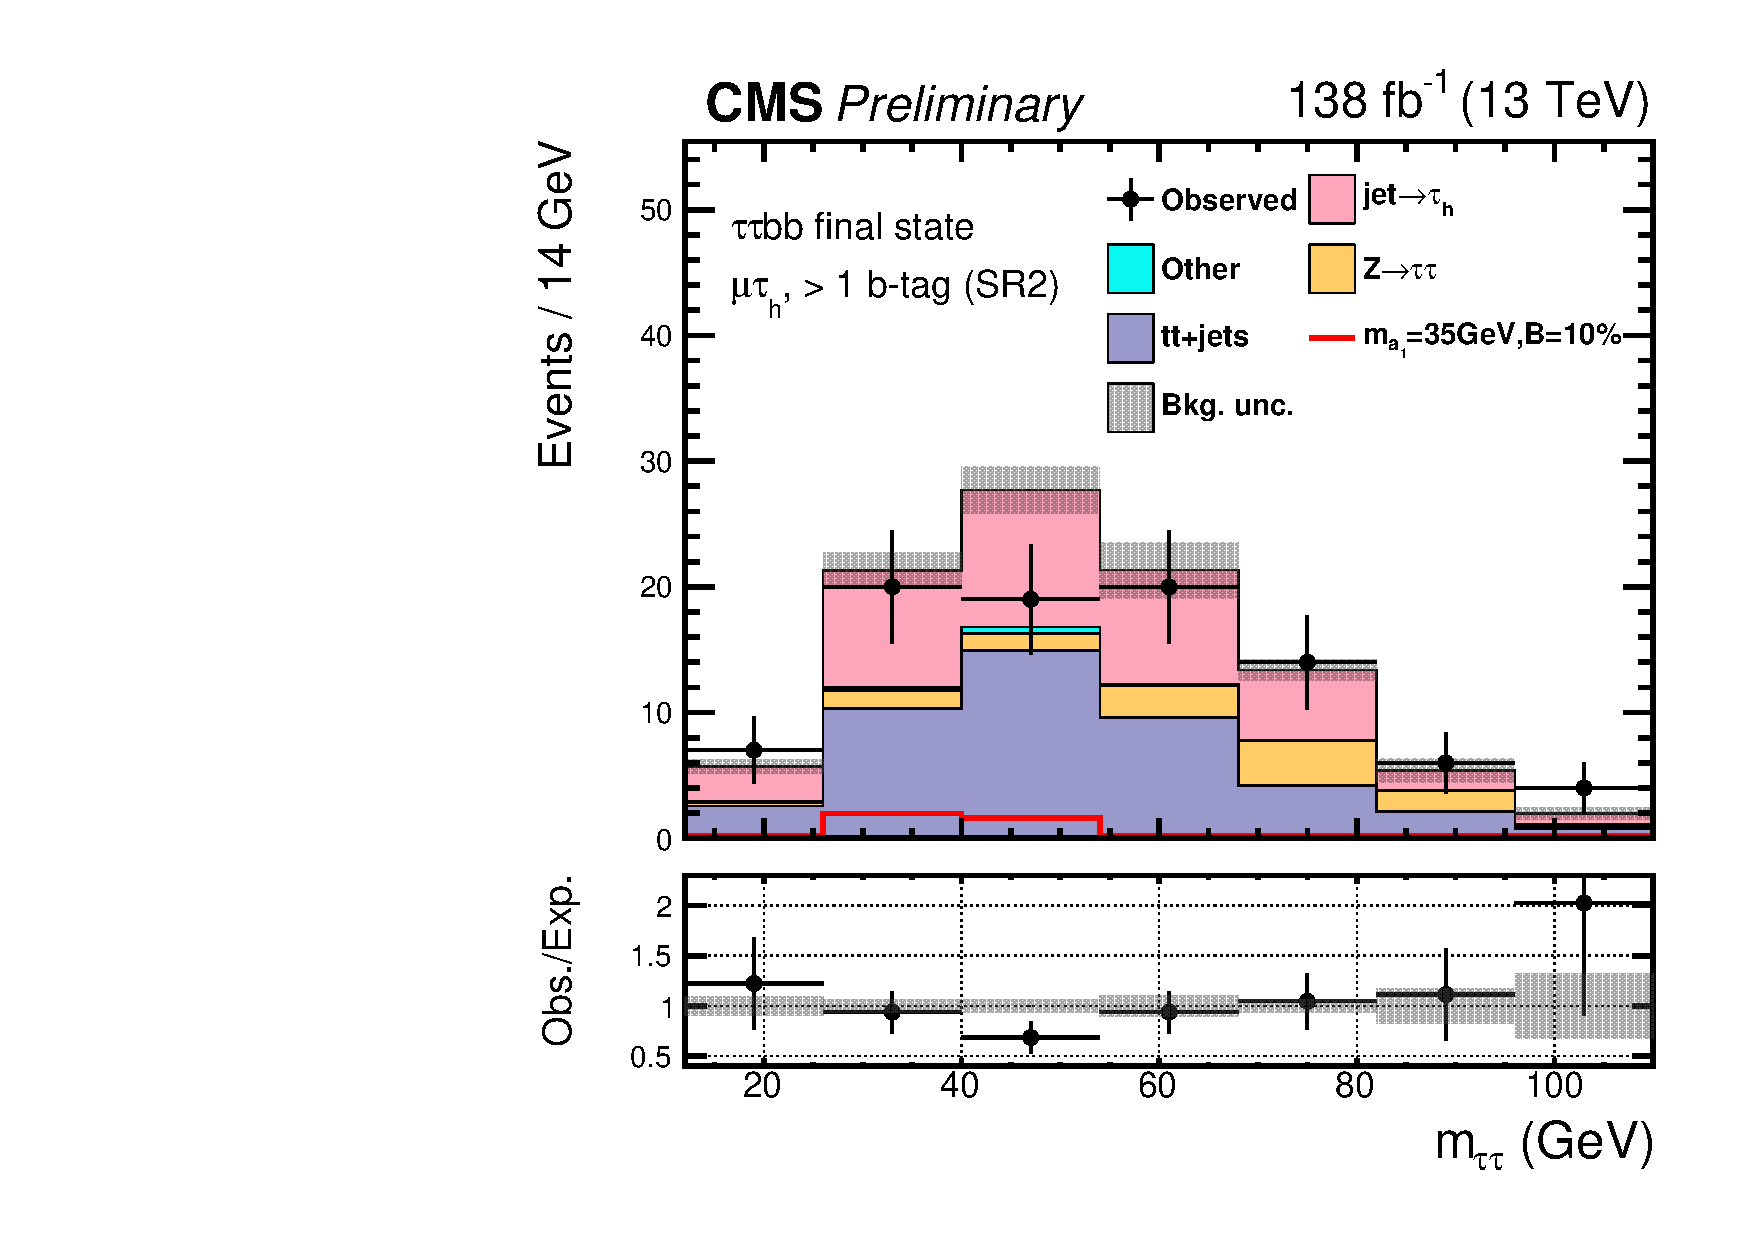
\includegraphics[width=0.32\textwidth]{figures/ch-14-results/mt_all_6_post_prelim-yes.pdf}\\
        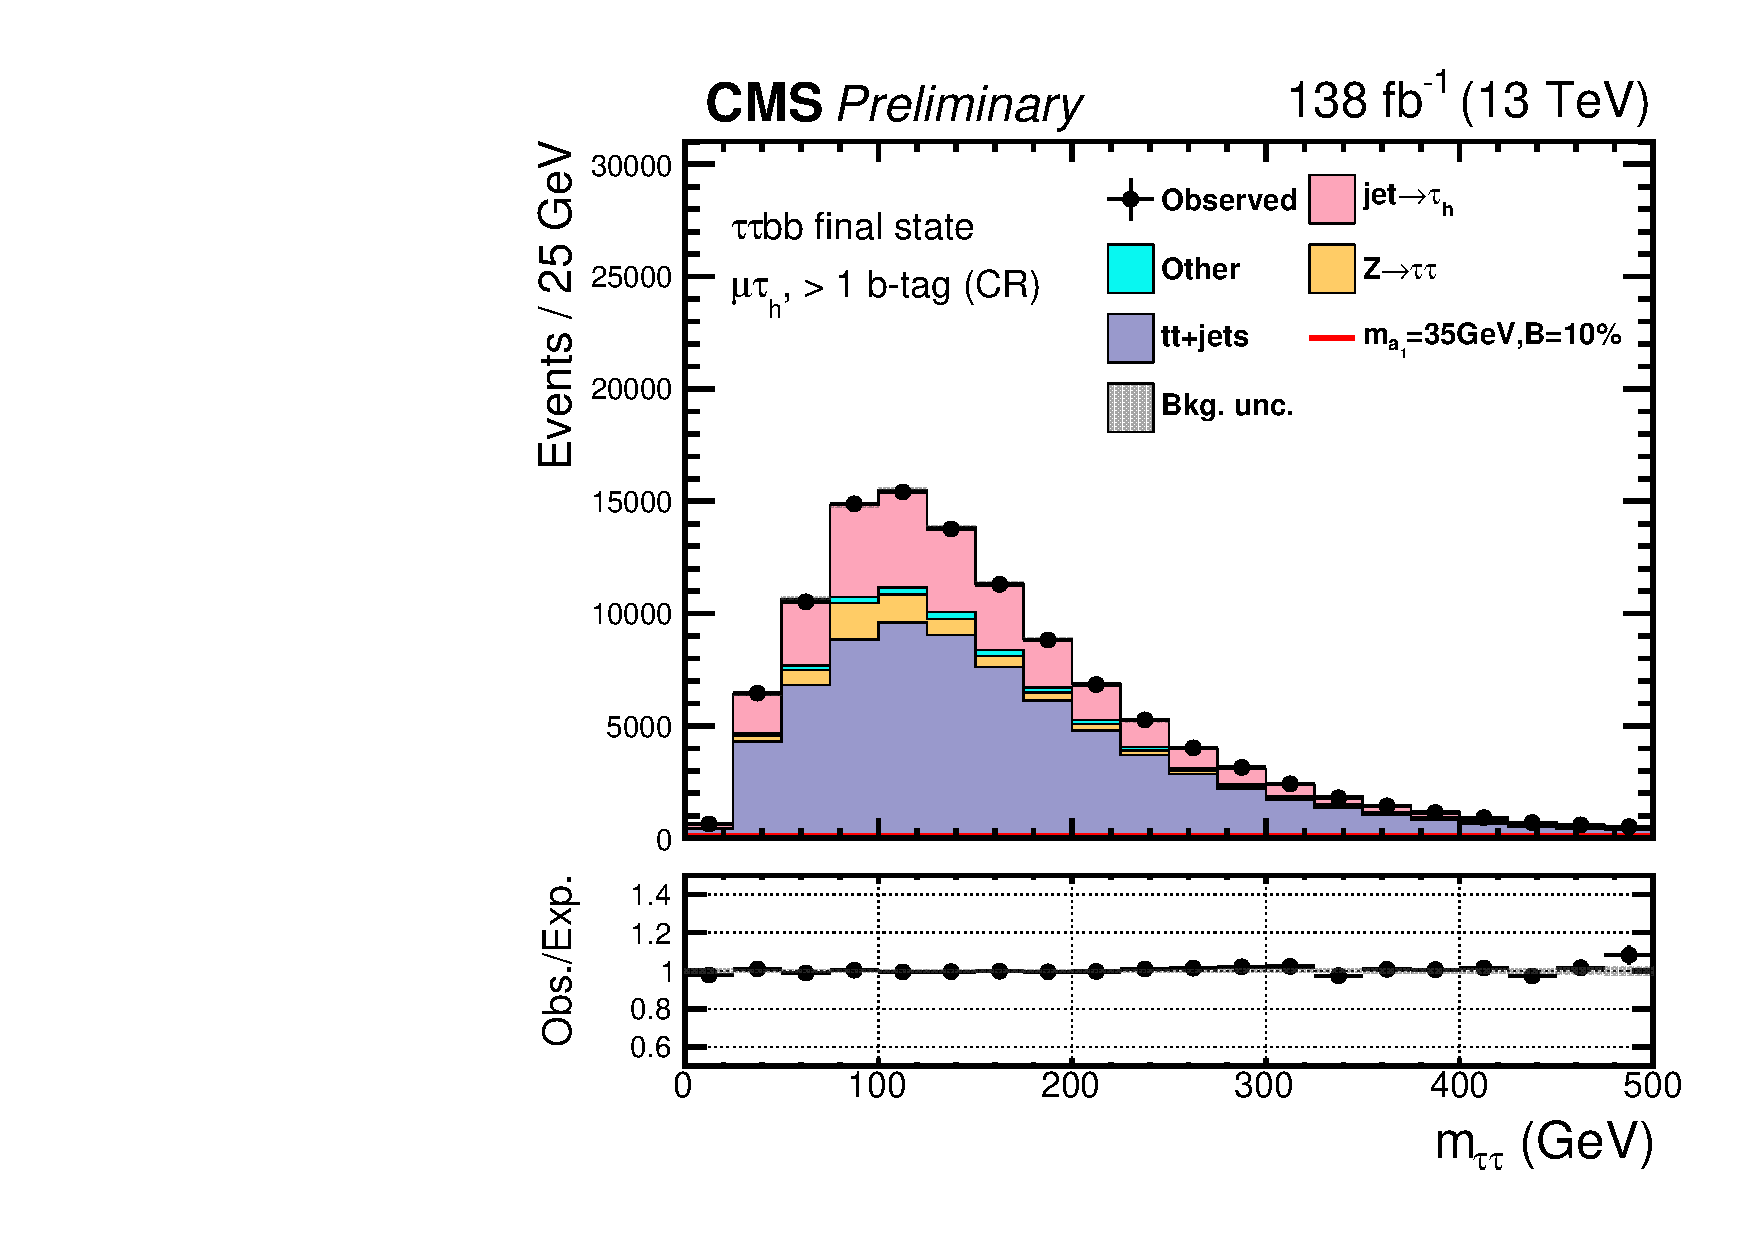
\includegraphics[width=0.32\textwidth]{figures/ch-14-results/mt_all_7_post_prelim-yes.pdf}
    \end{center}
    \caption[Postfit final $m_{\tau\tau}$ distributions in the $\mu\tau_{h}$ channel.]{Postfit final $m_{\tau\tau}$ distributions in the $\mu\tau_{h}$ channel \cite{CMS-AN-20-213}. Statistical and systematic uncertainties are included. \textit{Top row:} 1 b-tag jet categories: three signal regions (SR1, SR2, SR3). \textit{Middle row, left to right:} 1 b-tag jet categories: control region (CR), and 2 b-tag jet categories: two signal regions (SR1, SR2). \textit{Bottom:} 2 b-tag jet categories: control region (CR).}
    \label{fig:results_mtt_postfit_mtall}
\end{figure}

\begin{figure}[ht]
    \begin{center}
        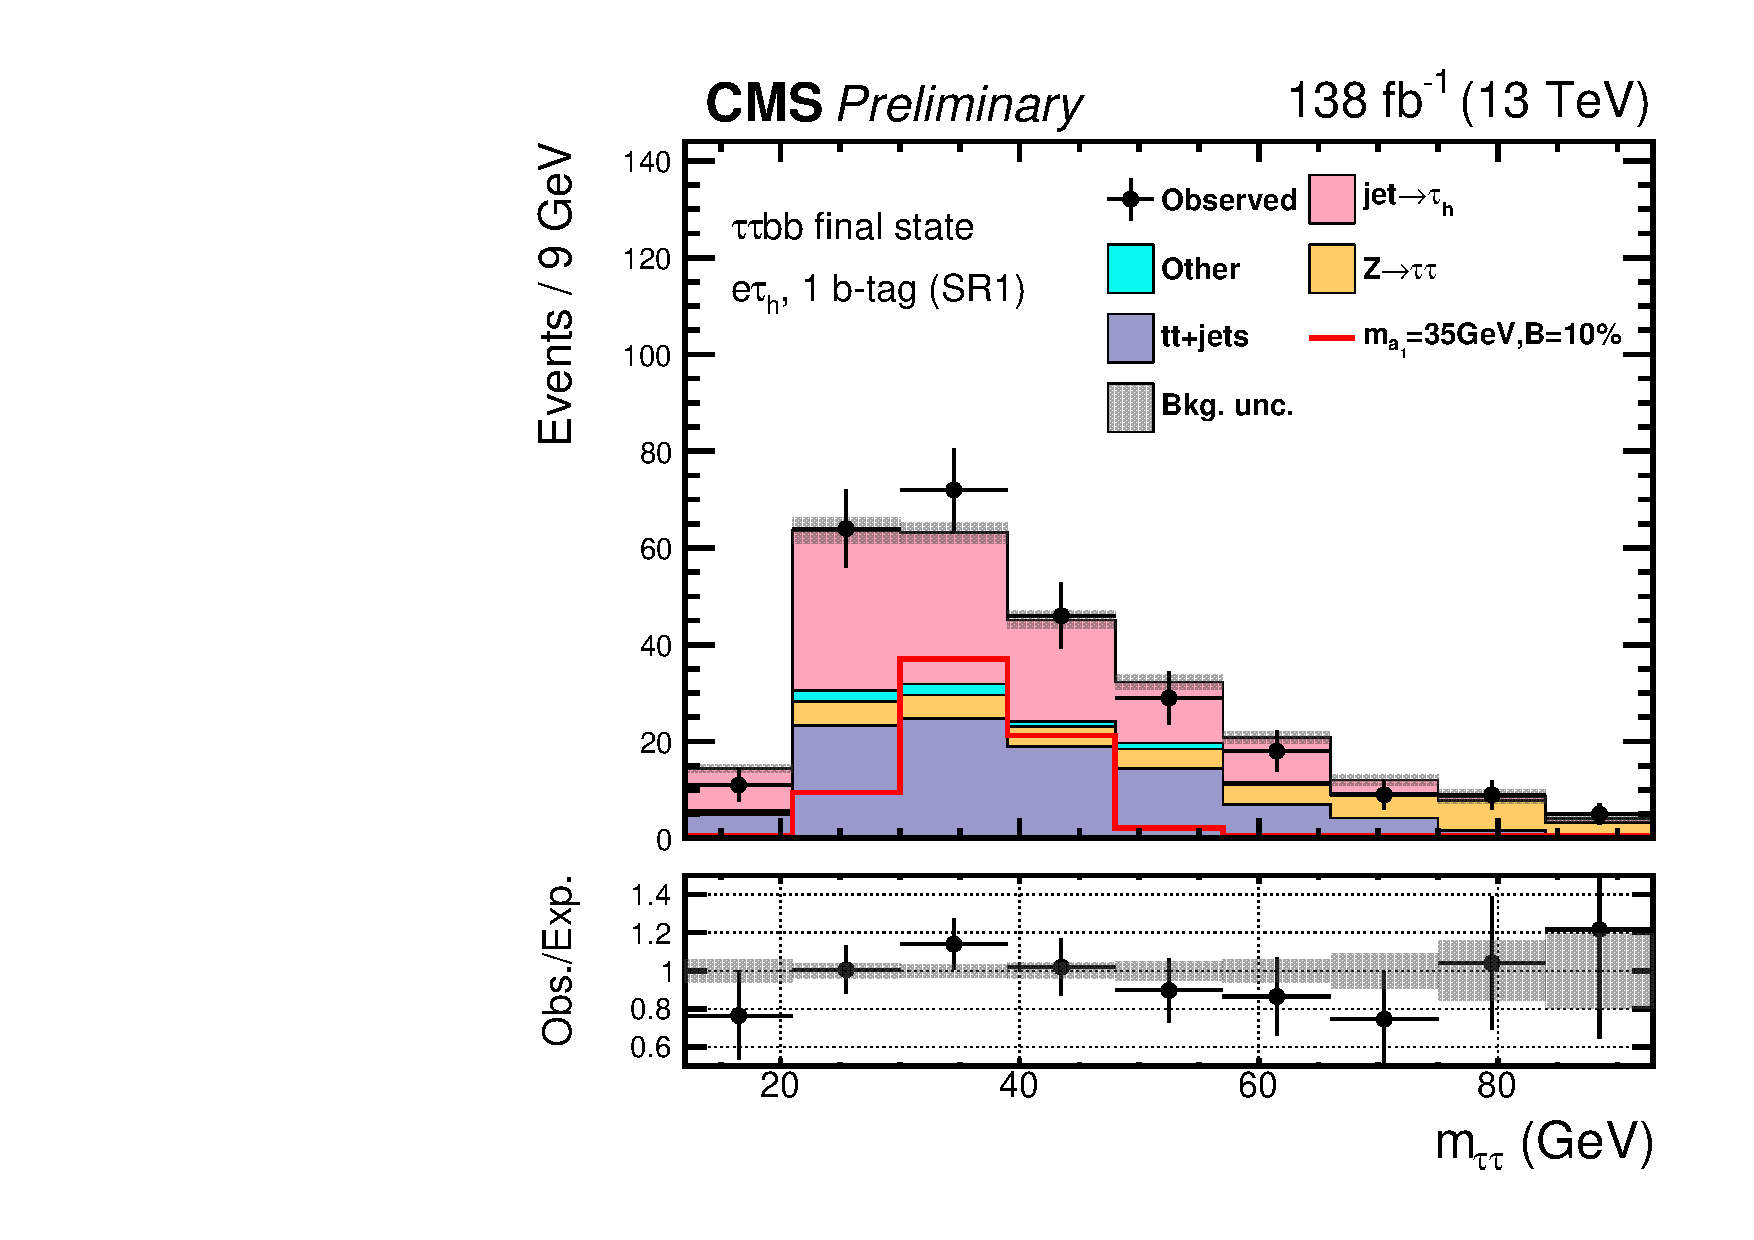
\includegraphics[width=0.32\textwidth]{figures/ch-14-results/et_all_1_post_prelim-yes.pdf}
        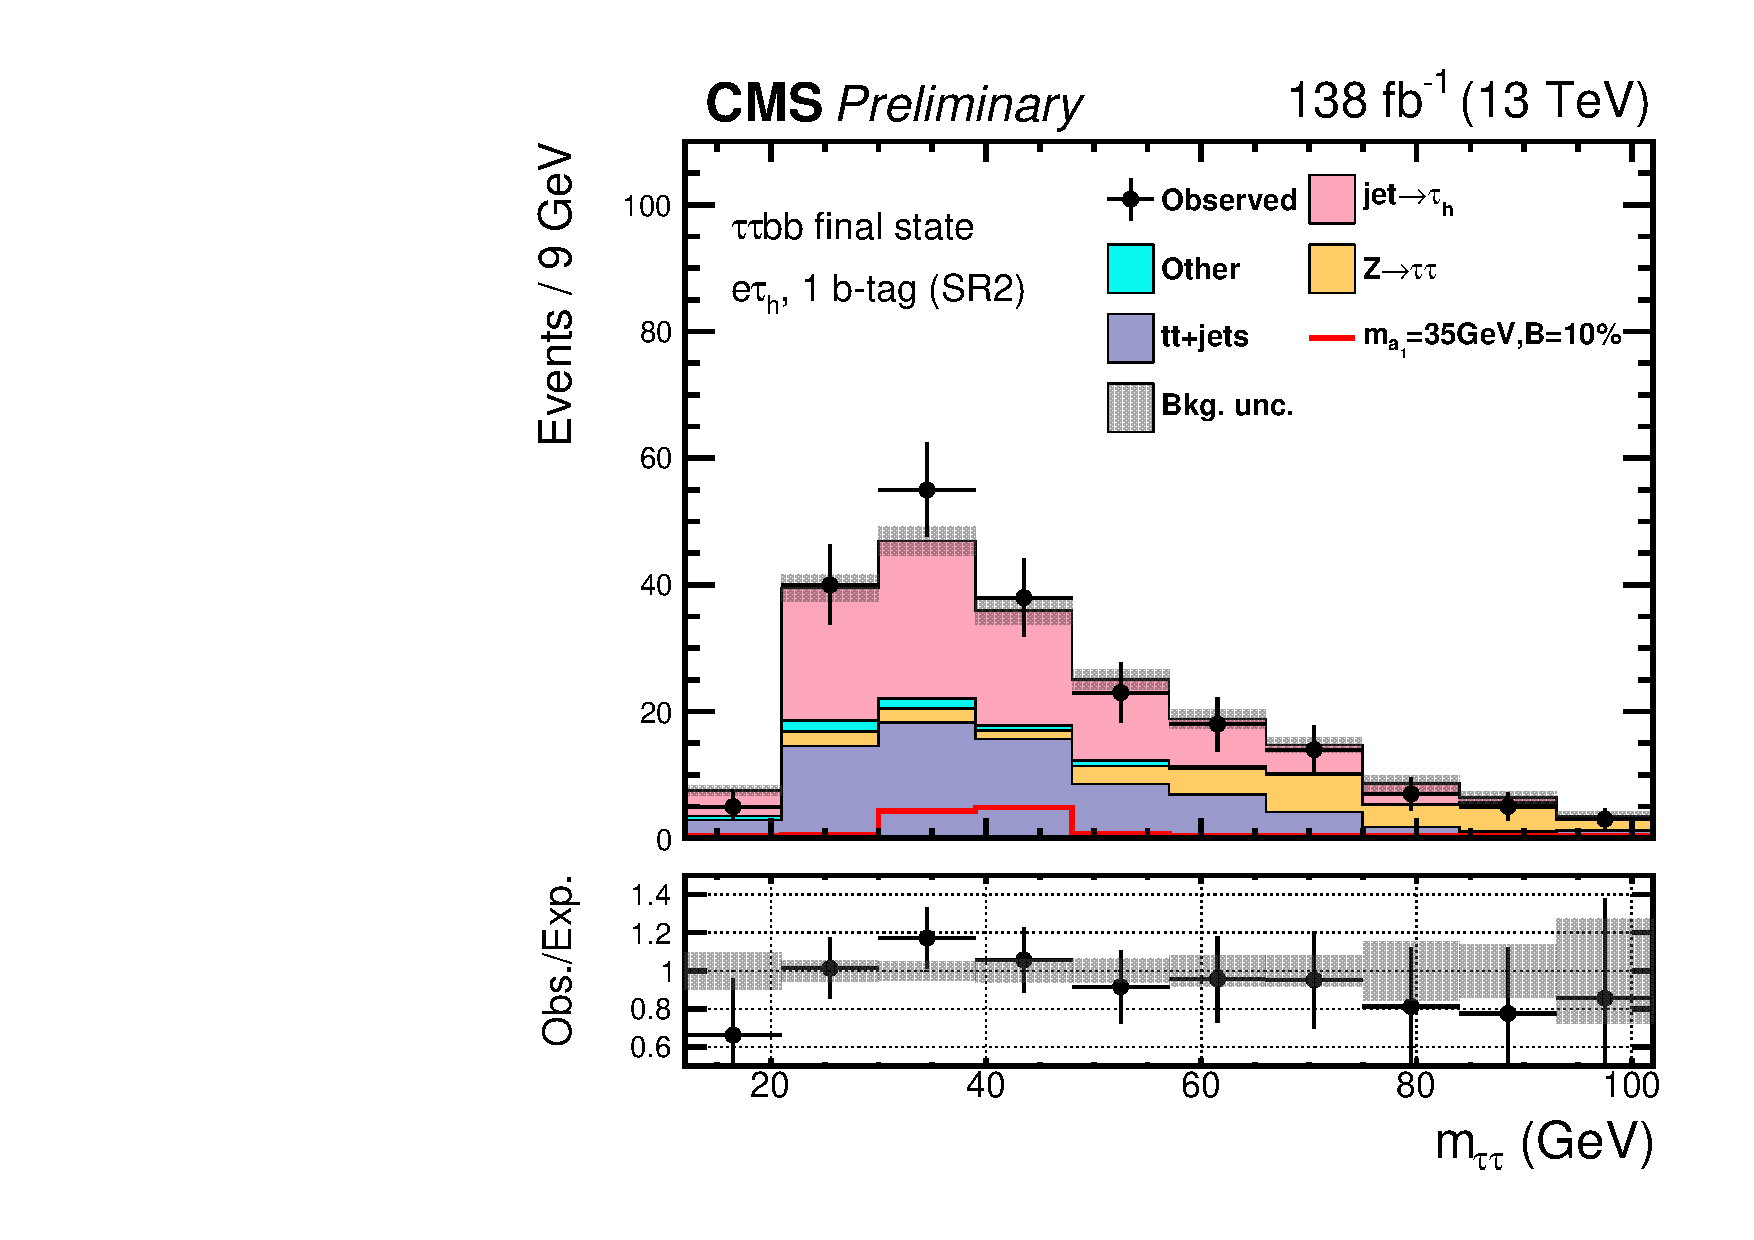
\includegraphics[width=0.32\textwidth]{figures/ch-14-results/et_all_2_post_prelim-yes.pdf}
        \includegraphics[width=0.32\textwidth]{figures/ch-14-results/et_all_3_post_prelim-yes.pdf}\\
        \includegraphics[width=0.32\textwidth]{figures/ch-14-results/et_all_4_post_prelim-yes.pdf}
        \includegraphics[width=0.32\textwidth]{figures/ch-14-results/et_all_5_post_prelim-yes.pdf}
        \includegraphics[width=0.32\textwidth]{figures/ch-14-results/et_all_6_post_prelim-yes.pdf}
    \end{center}
    \caption[Postfit final $m_{\tau\tau}$ distributions in the $e\tau_{h}$ channel]{Postfit final $m_{\tau\tau}$ distributions in the $e\tau_{h}$ channel \cite{CMS-AN-20-213}. Statistical and systematic uncertainties are included. \textit{Top row:} 1 b-tag jet categories: three signal regions (SR1, SR2, SR3). \textit{Bottom row, left to right:} 1 b-tag jet categories: control region (CR), and 2 b-tag jet categories: signal region (SR) and control region (CR).}
    \label{fig:results_mtt_postfit_etall}
\end{figure}

\begin{figure}[ht]
    \begin{center}
        \includegraphics[width=0.32\textwidth]{figures/ch-14-results/em_all_1_post_prelim-yes.pdf}
        \includegraphics[width=0.32\textwidth]{figures/ch-14-results/em_all_2_post_prelim-yes.pdf}
        \includegraphics[width=0.32\textwidth]{figures/ch-14-results/em_all_3_post_prelim-yes.pdf}\\
        \includegraphics[width=0.32\textwidth]{figures/ch-14-results/em_all_4_post_prelim-yes.pdf}
        \includegraphics[width=0.32\textwidth]{figures/ch-14-results/em_all_5_post_prelim-yes.pdf}
        \includegraphics[width=0.32\textwidth]{figures/ch-14-results/em_all_6_post_prelim-yes.pdf}\\
        \includegraphics[width=0.32\textwidth]{figures/ch-14-results/em_all_7_post_prelim-yes.pdf}
    \end{center}
    \caption[Postfit final $m_{\tau\tau}$ distributions in the $e\mu$ channel.]{Postfit final $m_{\tau\tau}$ distributions in the $e\mu$ channel \cite{CMS-AN-20-213}. Statistical and systematic uncertainties are included. \textit{Top row:} 1 b-tag jet categories: three signal regions (SR1, SR2, and SR3). \textit{Middle row, left to right:} 1 b-tag jet categories: control region (CR), and 2 b-tag jet categories: signal regions (SR1 and SR2). \textit{Bottom:} 2 b-tag jet categories: control region (CR).}
    \label{fig:results_mtt_postfit_emall}
\end{figure}


The 95\% CL exclusion limits on the signal strength of the branching ratio $\mathcal{B}(h \rightarrow aa \rightarrow bb\tau\tau)$, shown in percentage and normalized to the Standard Model Higgs production cross-section, is shown in Fig. \ref{fig:results_limits}. The pseudoscalar mass hypotheses $m_a$ between 15 GeV and 60 GeV are searched for in all channels. The $e\mu$ channel is the only channel that can provide sensitivity to the $m_a = 12$ GeV mass point, as its cut on the $\Delta R$ between the two $\tau$ legs is the smallest, which increases the signal acceptance for low mass signals.

No excess of events above the Standard Model expectations is observed. Combined expected (observed) limits between 1.4 and 5.6\% (1.7 and 7.6\%) are set for the pseudoscalar mass range between 12 and 60 GeV. The best sensitivity is attained at intermediate mass points, since the analysis targets a resolved signature: at low mass points, objects have a boosted signature, and at high mass points, the $m_{\tau\tau}$ distributions in signal have larger overlap with background distributions.

\begin{figure}[h!]
    \begin{center}
        \includegraphics[width=0.45\textwidth]{figures/ch-14-results/Limit_mt_prelim.pdf}
        \includegraphics[width=0.45\textwidth]{figures/ch-14-results/Limit_et_prelim.pdf}\\
        \includegraphics[width=0.45\textwidth]{figures/ch-14-results/Limit_em_prelim.pdf}
        \includegraphics[width=0.45\textwidth]{figures/ch-14-results/Limit_all_prelim.pdf}
    \end{center}
    \caption[95\% CL exclusion limits on B($h\rightarrow aa\rightarrow bb\tau\tau$) in \%.]{95\% CL exclusion limits on B($h\rightarrow aa\rightarrow bb\tau\tau$) in \%, for the combination of all years by channel (\textit{top left}: $\mu\tau_{h}$ channel, \textit{top right:} $e\tau_{h}$ channel, and \textit{Bottom left:} $e\mu$ channel) and the combination of all channels (\textit{bottom right}) \cite{CMS-AN-20-213}.}
    \label{fig:results_limits}
\end{figure}

The branching fraction of the two pseudoscalars depends on the 2HDM+S model type, the pseudoscalar mass $m_a$, and the ratio of the two vacuum expectation values $\tan\beta$. In Type I models, the branching fraction is independent of $\tan\beta$, while in Type III and IV models, it is a function of $m_a$ and $\tan\beta$. Using the predicted values of $B(a \rightarrow ff)$, the observed limits can be used to constrain the $\tan\beta$ vs. $m_a$ phase space. 


\section{Combination procedure with $bb\mu\mu$ final state}
\label{section:ch-13-combination-procedure-with-bbmumu}
A combination of the results from $bb\tau\tau$ is performed with the analysis for the $h \rightarrow aa \rightarrow bb\mu\mu$ final state \cite{CMS-AN-21-058-bbmumu}. While the $bb\mu\mu$ final state has a small branching ratio, it provides competitive results due to the excellent di-muon resolution measured by CMS. The $bb\mu\mu$ analysis uses an unbinned fit to the data using the di-muon mass $m_{\mu\mu}$ distribution.

A combination is possible because the two final states use event selections that are orthogonal to each other, as the $bb\tau\tau$ channels veto events with extra leptons. Several systematic uncertainties are treated as correlated: the integrated luminosity normalization,the b-tagging scale factor, the scale factors related to muon reconstruction, identification, and trigger efficiencies, the inefficiency in the ECAL trigger readout, and the theoretical uncertainties related to signal modeling.

The dimuon and ditau mass distributions ($m_{\mu\mu}$ and $m_{\tau\tau}$) are compared to the data in a combined maximum likelihood fit to derive upper limits on B($h\rightarrow aa$). 

\section{Results from combination}

The observed limits at 95\% CL on B($h \rightarrow aa$) for different 2HDM+S scenarios are shown for the $bb\mu\mu$ analysis in Fig. \ref{fig:results_limits_mmbb}, the $bb\tau\tau$ analysis in Fig. \ref{fig:results_limits_ttbb}, and the combined analyses in Fig. \ref{fig:results_limits_combined}. For 2HDM+S Types II, III, and IV, exclusion limits are set as a function of $\tan\beta$ and $m_{a}$, and are shown in Fig. \ref{fig:results_limits_combined_2D}.

The most stringent constraints are observed for the Type III model, which predicts combined branching fractions between 0.47 and 0.42 for $\tan\beta = 2.0$ and values of $m_{a}$ between 15 and 60 GeV, while the 95\% CL upper limits are between 0.08 and 0.03. For the Type IV model, the predicted branching fractions from theory are between 0.26 and 0.20 for $\tan\beta = 0.6$ for values of $m_{a}$ between 15 and 60 GeV, and the 95\% CL observed upper limits are between 0.12 and 0.05. 

\begin{figure}[ht]
    \begin{center}
      \includegraphics[width=0.5\textwidth]{figures/ch-14-results/HAA_bbmm_all_prelim.pdf}
    \end{center}
    \caption[Observed 95\% CL upper limits on B$(h \rightarrow aa)$ in \%, for the $bb\mu\mu$ channel using the full Run 2 integrated luminosity of 138 $fb^{-1}$ for different 2HDM+S models.]{Observed 95\% CL upper limits on B$(h \rightarrow aa)$ in \%, for the $bb\mu\mu$ channel using the full Run 2 integrated luminosity of 138 $fb^{-1}$ for different 2HDM+S models. Limits on the Type I 2HDM+S model do not depend on $\tan\beta$ \cite{CMS-AN-20-213}.}
      \label{fig:results_limits_mmbb}
  \end{figure}
  \begin{figure}[h!]
    \begin{center}
      \includegraphics[width=0.5\textwidth]{figures/ch-14-results/HAA_bbtt_all_prelim.pdf}
    \end{center}
    \caption[Observed 95\% CL upper limits on B$(h \rightarrow aa)$ in \%, for the $bb\tau\tau$ channel using the full Run 2 integrated luminosity of 138 $fb^{-1}$ for different 2HDM+S models.]{Observed 95\% CL upper limits on B$(h \rightarrow aa)$ in \%, for the $bb\tau\tau$ channel using the full Run 2 integrated luminosity of 138 $fb^{-1}$ for different 2HDM+S models. Limits on the Type I 2HDM+S model do not depend on $\tan\beta$ \cite{CMS-AN-20-213}.}
      \label{fig:results_limits_ttbb}
  \end{figure}
  \begin{figure}[h!]
    \begin{center}
      \includegraphics[width=0.5\textwidth]{figures/ch-14-results/HAA_comb_all_prelim.pdf}
    \end{center}
    \caption[Observed 95\% CL upper limits on $\mathcal{B}(h\to aa)$ in \%, for the combination of $bb\mu\mu$ and $bb\tau\tau$ channels using the full Run 2 integrated luminosity of 138 $fb^{-1}$ for different 2HDM+S models.]{Observed 95\% CL upper limits on $\mathcal{B}(h\to aa)$ in \%, for the combination of $bb\mu\mu$ and $bb\tau\tau$ channels using the full Run 2 integrated luminosity of 138 $fb^{-1}$ for different 2HDM+S models. Limits on the Type I 2HDM+S model do not depend on $\tan\beta$ \cite{CMS-AN-20-213}.}
      \label{fig:results_limits_combined}
  \end{figure}
  


\begin{figure}[h]
    \begin{center}
      \includegraphics[width=0.32\textwidth]{figures/ch-14-results/HAA_comb_II_prelim.pdf}
      \includegraphics[width=0.32\textwidth]{figures/ch-14-results/HAA_comb_III_prelim.pdf}
      \includegraphics[width=0.32\textwidth]{figures/ch-14-results/HAA_comb_IV_prelim.pdf}
    \end{center}
    \caption[Observed 95\% CL upper limits on $\mathcal{B}(h\to aa)$ in \%, for the combination of $bb\mu\mu$ and $bb\tau\tau$ channels using the full Run 2 integrated luminosity of 138 $fb^{-1}$ for Type II (\textit{left}), Type III (\textit{middle}), and Type IV (\textit{right}) 2HDM+S in the $\tan\beta$ vs. $m_a$ phase space.]{Observed 95\% CL upper limits on $\mathcal{B}(h\to aa)$ in \%, for the combination of $bb\mu\mu$ and $bb\tau\tau$ channels using the full Run 2 integrated luminosity of 138 $fb^{-1}$ for Type II (\textit{left}), Type III (\textit{middle}), and Type IV (\textit{right}) 2HDM+S in the $\tan\beta$ vs. $m_a$ phase space. The contours corresponding to branching ratios of 100\% and 34\% are drawn using dashed lines, 34\% corresponding to the previous upper limit on Higgs to BSM particle decays during Run 1. Linear extrapolation has been used between different points on the figures \cite{CMS-AN-20-213}.}
      \label{fig:results_limits_combined_2D}
  \end{figure}
  
The combined analyses' results are also shown in summary plots alongside the other current CMS results for 2HDM+S limits: for type I in Fig. \ref{fig:summary_plot_type_I}, for type II with $\tan\beta = 2.0$ in Fig. \ref{fig:summary_plot_typeII_tan_beta_2p0}, and for type III with $\tan\beta = 2.0$ in Fig. \ref{fig:summary_plot_typeIII_tan_beta_2p0}. In other scenarios, e.g. type III with $\tan\beta = 5.0$, more stringent limits are set by analyses in other final states, $\mu\mu\tau\tau$ in this case. Other summary plots can be found at \cite{twiki_2HDM+S_summary-plots}.

\begin{figure}[h]
    \begin{center}
      \includegraphics[width=0.6\textwidth]{figures/ch-14-results/summary_plot_full_run2_plot_BRaa_Type1.pdf}
    \end{center}
    \caption[95\% limits on $\frac{\sigma(h)}{\sigma_{\text{SM}}} \times \mathcal{B}(h \rightarrow aa)$ in the 2HDM+S type-I scenario for exotic Higgs decay searches, performed with data collected at 13 TeV.]{95\% limits on $\frac{\sigma(h)}{\sigma_{\text{SM}}} \times \mathcal{B}(h \rightarrow aa)$ in the 2HDM+S type-I scenario for exotic Higgs decay searches, performed with data collected at 13 TeV. The combined result for $h\rightarrow aa \rightarrow \ell\ell bb$ \cite{CMS-HIG-22-007} is shown in purple.}
      \label{fig:summary_plot_type_I}
  \end{figure}
  \begin{figure}[h]
    \begin{center}
      \includegraphics[width=0.6\textwidth]{figures/ch-14-results/summary_plot_full_run2_plot_BRaa_Type2_tanbeta2.pdf}
    \end{center}
    \caption[95\% limits on $\frac{\sigma(h)}{\sigma_{\text{SM}}} \times \mathcal{B}(h \rightarrow aa)$ in the 2HDM+S type-II scenario with $\tan\beta = 2.0$ for exotic Higgs decay searches, performed with data collected at 13 TeV.]{95\% limits on $\frac{\sigma(h)}{\sigma_{\text{SM}}} \times \mathcal{B}(h \rightarrow aa)$ in the 2HDM+S type-II scenario with $\tan\beta = 0.0$ for exotic Higgs decay searches, performed with data collected at 13 TeV. The combined result for $h\rightarrow aa \rightarrow \ell\ell bb$ \cite{CMS-HIG-22-007} is shown in purple, representing the most stringent limits in the probed mass ranges in this scenario.}
      \label{fig:summary_plot_typeII_tan_beta_2p0}
  \end{figure}
  \begin{figure}[h]
    \begin{center}
      \includegraphics[width=0.6\textwidth]{figures/ch-14-results/summary_plot_full_run2_plot_BRaa_Type3_tanbeta2.pdf}
    \end{center}
    \caption[95\% limits on $\frac{\sigma(h)}{\sigma_{\text{SM}}} \times \mathcal{B}(h \rightarrow aa)$ in the 2HDM+S type-III scenario with $\tan\beta = 2.0$ for exotic Higgs decay searches, performed with data collected at 13 TeV.]{95\% limits on $\frac{\sigma(h)}{\sigma_{\text{SM}}} \times \mathcal{B}(h \rightarrow aa)$ in the 2HDM+S type-III scenario with $\tan\beta = 2.0$ for exotic Higgs decay searches, performed with data collected at 13 TeV. The combined result for $h\rightarrow aa \rightarrow \ell\ell bb$ \cite{CMS-HIG-22-007} is shown in purple.}
      \label{fig:summary_plot_typeIII_tan_beta_2p0}
  \end{figure}
  

% \appendix
% \chapter{Code}
% \input{./Chapters/code}

\bibliography{Thesis} \label{bib}
%\nocite{*}

\end{document}



